%-----------------------------------------------------------------
% Preamble
%------------------------------------------------------------------
\documentclass[12pt,a4paper,twoside,openright]{book}
\usepackage{mathptmx} % times no roman-like font
\usepackage[left=30mm, right=25mm, top=25mm, bottom=25mm]{geometry} % margins
\usepackage{setspace}
\usepackage{fancyhdr}
\pagestyle{fancy}
\renewcommand{\baselinestretch}{1.15}
\usepackage[utf8]{inputenc}
\usepackage{graphicx}
\graphicspath{{figures/}}
\def\blankpage{%
      \clearpage%
      \thispagestyle{empty}%
      \null%
      \clearpage}

%-----------------------------------------------------------------
% Packages
%------------------------------------------------------------------
\renewcommand{\chaptermark}[1]{\markboth{\MakeUppercase{\thechapter. #1 }}{}}
\renewcommand{\sectionmark}[1]{\markright{\thesection\ #1}}
\usepackage{titlesec}
\fancyhf{}
\fancyhead[RO]{\bfseries\rightmark}
\fancyhead[LE]{\bfseries\leftmark}
\setlength{\headheight}{15pt}
\fancyfoot[C]{\thepage}
\renewcommand{\headrulewidth}{0pt}
\renewcommand{\footrulewidth}{0pt}
\addtolength{\headheight}{0.5pt}
\fancypagestyle{plain}{
  \fancyhead{}
  \renewcommand{\headrulewidth}{0pt}
}
\usepackage{hyperref}
\usepackage{graphicx}
\usepackage[nottoc]{tocbibind}
\usepackage[backend=biber,style=numeric-comp,maxcitenames=1,autocite=inline,natbib=true,sorting=none]{biblatex}
\addbibresource{references.bib}
\usepackage{indentfirst}
\setlength{\parskip}{1em}
\setcounter{tocdepth}{4}
\setcounter{secnumdepth}{4}
\usepackage{enumitem}
\usepackage[font=footnotesize]{caption}
\usepackage[toc,page]{appendix}
\usepackage{pdfpages}
\usepackage{fmtcount}
\usepackage{url}
\usepackage{amsmath}
\usepackage{bm}
\usepackage[utf8]{inputenc}
\usepackage{filecontents}
\usepackage{float}
\raggedbottom
\usepackage{subcaption}
\usepackage{eurosym}
\usepackage{booktabs}
\usepackage[T1]{fontenc}
\usepackage[acronym]
\makeatletter

\def\cleardoublepage{\clearpage\if@twoside \ifodd\c@page\else
    \hbox{}
    \thispagestyle{plain}
    \newpage
    \if@twocolumn\hbox{}\newpage\fi\fi\fi}
\makeatother \clearpage{\pagestyle{plain}\cleardoublepage}

\providecommand{\keywords}[1]{\textbf{Keywords:} #1}
\providecommand{\keywordsP}[1]{\textbf{Palavras chave:} #1}
\newcommand{\secref}[1]{\autoref{#1}. \nameref{#1}}
\usepackage{lscape}
\usepackage{adjustbox}
\usepackage{booktabs}
\usepackage{multirow}
\hypersetup{hidelinks}
\usepackage{longtable}
\usepackage{acronym} 
\usepackage{amssymb}
\usepackage{pifont}
\usepackage[symbol]{footmisc}
\renewcommand{\thefootnote}{\fnsymbol{footnote}}


%-----------------------------------------------------------------
% Begin Document
%------------------------------------------------------------------

\begin{document}
\begin{sloppy}
\frontmatter

%-----------------------------------------------------------------
% Cover
%------------------------------------------------------------------
\begin{titlepage}
    \begin{center}
        UNIVERSIDADE DE LISBOA\\
        FACULDADE DE MEDICINA
        
        \vspace{1cm}
        
        {
\includegraphics{figures/cover/UL-VerticalPositivo.png}}
        
        \vspace{1cm}

        \huge
        \textbf{Towards accreditation in metagenomics \\[1ex] for clinical microbiology}
        \normalsize
        
        \vspace{1cm}
        
        \large
        Catarina Inês Marques de Sousa Mendes
        \normalsize
        
        \vspace{1cm}
        
        Orientador: Doutor João André Nogueira Custódio Carriço\\
        Co-orientador: Professor Doutor Mário Nuno Ramos de Almeida Ramirez
        
        \vfill
        
        Tese especialmente elaborada para obtenção do grau de Doutor em Ciências e Tecnologias da Saúde, especialidade em Biologia Computacional\\
        
        \vspace{0.8cm}
        
        2023
        
    \end{center}
\end{titlepage}
\clearpage \thispagestyle{empty}\mbox{}\clearpage

%-----------------------------------------------------------------
% Folha de rosto
%------------------------------------------------------------------
\begin{titlepage}
    \begin{center}
        UNIVERSIDADE DE LISBOA\\
        FACULDADE DE MEDICINA
        
        \vspace{1cm}
        
        {
\includegraphics{figures/cover/UL-VerticalPositivo.png}}
        
        \vspace{1cm}

        \huge
        \textbf{Towards accreditation in metagenomics \\[1ex] for clinical microbiology}
        \normalsize
        
        \vspace{0.8cm}
        
        \large
        Catarina Inês Marques de Sousa Mendes
        \normalsize
        
        \vspace{0.8cm}
        
        Orientador: Doutor João André Nogueira Custódio Carriço\\
        Co-orientador: Professor Doutor Mário Nuno Ramos de Almeida Ramirez
        
        \vspace{0.8cm}
        
        Documento provisório\\
        Tese especialmente elaborada para obtenção do grau de Doutor em Ciências e Tecnologias da Saúde, especialidade em Biologia Computacional\\
        
        \vspace{0.5cm}
        
        Fundação para a Ciência e Tecnologia \\ 
        SFRH/BD/129483/2017 and COVID/BD/152583/2022
        
        \vspace{0.2cm}
        
        2022
    \end{center}
\end{titlepage}
\clearpage \thispagestyle{empty}\mbox{}\clearpage

%-----------------------------------------------------------------
% Disclaimer
%------------------------------------------------------------------
\newpage
\thispagestyle{empty}
\vspace*{\fill}
As opiniões expressas nesta publicação são da exclusiva responsabilidade do seu autor.
\blankpage

%-----------------------------------------------------------------
% Dedication
%------------------------------------------------------------------
\newpage
\thispagestyle{empty}
\vspace*{3cm}
\begin{center}
\emph{"The greatest adventure is what lies ahead.\\
Today and tomorrow are yet to be said.\\
The chances, the changes are all yours to make.\\
The mould of your life is in your hands to break."} \\
\end{center} 
\begin{flushright}-J. R. R. Tolkien, The Hobbit\end{flushright}
\clearpage \thispagestyle{empty}\mbox{}\clearpage


%-----------------------------------------------------------------
% Acknowledgements
%------------------------------------------------------------------
\newpage
\thispagestyle{plain}
\addcontentsline{toc}{chapter}{Acknowledgements}
\chapter*{Acknowledgements}
\clearpage \thispagestyle{empty}\mbox{}\clearpage

%-----------------------------------------------------------------
% Summary
%------------------------------------------------------------------
\newpage
\thispagestyle{plain}
\addcontentsline{toc}{chapter}{Summary}
\chapter*{Summary}

\keywords{one, two, three, four, five}
\clearpage \thispagestyle{empty}\mbox{}\clearpage

%-----------------------------------------------------------------
% Resumo
%------------------------------------------------------------------
\newpage
\thispagestyle{plain}
\addcontentsline{toc}{chapter}{Resumo}
\chapter*{Resumo}

\keywords{um, dois, três, quatro, cinco}
\clearpage \thispagestyle{empty}\mbox{}\clearpage

%-----------------------------------------------------------------
% Thesis Outline
%------------------------------------------------------------------
\newpage
\thispagestyle{plain}
\addcontentsline{toc}{chapter}{Thesis Outline}
\chapter*{Thesis Outline}
The work described in the present thesis intends to evaluate the use of bioinformatics methods for the analysis of metagenomic data to allow the rapid identification, virulence analysis and antimicrobial susceptibility prediction of pathogens with clinical relevance. Ultimately, the applicability of metagenomic methods is to be evaluated in a clinical setting as an alternative to current gold standards. Given the dependence of these methodologies on bioinformatics post-processing of the raw data obtained, the major applications and pitfalls of metagenomics are yet to be identified. 

The thesis organisation reflects the six publications included, with each of the results chapters containing mostly the content of the publication indicated at the start of that chapter. Given this option, in addition to an introductory preface giving the context of the work performed, each results chapter has its own introduction, materials and methods, discussion, and conclusion. Overall, the thesis comprises 10 chapters, organised as follows: The first, second to last and last chapters include the general introduction, general discussion and main conclusions of the work developed in this thesis, respectively; while the body of the thesis work, corresponding to chapters 2 to 8, is organised into four parts aggregating chapters under a broader topic, numbered from I to IV.

In \textbf{Chapter 1} the issues addressed throughout the thesis are put into context, highlighting the current impact of genomics in clinical microbiology, both as a diagnostic or a surveillance tool. The entire process in clinical microbiology for bacterial and viral infections is showcased through its different approaches over time: classical biochemical and molecular methods, whole-genome sequencing, and sequencing through metagenomics, both metataxonomics and shotgun, with a focus on the computational requirements necessary. This chapter elaborates on the evolution of whole-genome sequencing to metagenomic approaches, introducing the possibility of identifying and characterising a potential pathogen without the need for a priori knowledge of the causative agent of disease. The importance of the bioinformatics analysis of this data was underlined, showcasing its complexity and major pitfalls, such as reproducibility and transparency of the analysis methods.   

\textbf{Part I} of the results, named “\textit{Applying metagenomics in the clinical context}”, includes \textbf{Chapters 2, 3 and 4}, where metagenomics is applied to both clinical and environmental samples. In the two first chapters, the performance of metagenomics to identify pathogens and antimicrobial resistance genes was evaluated. Importantly it was recognized that there was a lack of standardisation in the bioinformatic metagenomics analysis, so a fully reproducible workflow was developed for the streamlined analysis of human samples for genomic characterization in the context of Dengue infections, as a model for other applications.

\textbf{Chapter 2} consists of the application of the shotgun metagenomics approach to nine body fluid samples and one tissue sample from patients at the University Medical Center Groningen (UMCG) as to compare against current golden standards practises in the diagnosis of disease. In this study, the accuracy and reliability of the bioinformatics analyses were evaluated and compared against the results obtained from traditional culture methods. Our aim was to evaluate the applicability of shotgun metagenomics in a routine diagnostic setting, and not only in cases where traditional methods fail to provide an answer. Most pathogens identified by culture were also identified by metagenomics. Substantial differences were noted between the taxonomic classification tools, highlighting the potential and limitations of shotgun metagenomics as a diagnostic tool. The fact that, when applying shotgun metagenomics to diagnostics, the results are highly dependent on the tools, and especially the database that was chosen for the analysis greatly impacts its applicability in a clinical setting. This chapter is included in the following publication:\textit{ N. Couto, L. Schuele, E.C. Raangs, M. P. Machado, \underline{C. I. Mendes}, T. F. Jesus, M. Chlebowicz,  S. Rosema, M. Ramirez, J. A. Carriço, I. B. Autenrieth, A. W. Friedrich, S. Peter and J. W. Rossen. Critical steps in clinical shotgun metagenomics for the concomitant detection and typing of microbial pathogens. Sci Rep 8, 13767 (2018). DOI: \url{https://doi.org/10.1038/s41598-018-31873-w}}

\textbf{Chapter 3} describes the application of both second and third-generation sequencing technologies, also known as next-generation and long-read sequencing, to eight tap-water samples collected at the University Medical Center Groningen. Our aim was to evaluate the applicability of shotgun metagenomics, but this time in a surveillance setting. Building on the findings from Chapter 2, a hybrid assembly approach was used to increase resolution power. In this sample a new variant of a colistin resistance (mcr) determinant was detected, named \textit{mcr-5.4}, and through hybrid assembly leveraging both short and long-read sequences, its context was determined, albeit with questionable success. This chapter is included in the following publication: \textit{G. Fleres, N. Couto, L. Schuele, M. A. Chlebowicz, \underline{C. I. Mendes}, L. W. M. van der Sluis, J. W. A. Rossen, A. W Friedrich, S. García-Cobos, Detection of a novel mcr-5.4 gene variant in hospital tap water by shotgun metagenomic sequencing, Journal of Antimicrobial Chemotherapy, Volume 74, Issue 12, December 2019, Pages 3626–3628.  DOI: \url{https://doi.org/10.1093/jac/dkz363.}}

With the lessons learnt in Chapters 2 and 3, we developed in \textbf{Chapter 4} DEN-IM, a one-stop, user-friendly, containerised and reproducible workflow for the analysis of Dengue virus short-read sequencing data from both amplicon and shotgun metagenomics approaches. This takes into particular consideration the dependency on software and database versions used in the metagenomic bioinformatics downstream analysis in the results obtained. Dengue virus represents a public health threat and economic burden in affected countries, with the risk of exposure, increasing, not only driven by travel to endemic regions but also due to the broader dissemination of the mosquito vector, making the burden of dengue very significant. This makes it a particularly relevant target organism for the development of a straightforward workflow for both the identification and characterization of the virus. DEN-IM was designed to perform a comprehensive analysis in order to generate either de novo assemblies or consensus of full viral coding sequences and to identify their serotype and genotype, including the identification of co-infection cases whose prevalence is increasingly found in highly endemic areas. It was developed in Nextflow,  a simple and scalable workflow management system. All tools and dependencies are provided in Docker containerised images. All these steps ensure reproducibility and transparency of the bioinformatic process. This chapter is included in the following publication: \textit{\underline{C. I. Mendes}\footnote[1]{These authors contributed equally to this work.}, E. Lizarazo$^*$, M. P. Machado, D. N. Silva, A. Tami, M. Ramirez, N. Couto, J. W. A. Rossen, J. A. Carriço, DEN-IM: dengue virus genotyping from amplicon and shotgun metagenomic sequencing. Microbial Genomics, Volume 6, Issue 3, March 2020. DOI: \url{https://doi.org/10.1099/mgen.0.000328.}}

\textbf{Part II} includes only \textbf{Chapter 5}, and is named “\textit{The impact of de novo assemblers in metagenomics}”. A key process in metagenomic data analysis is the de novo assembly of raw sequence data since it allows recovering contigs representing the replicons present in the sample, be it genomes, plasmids, or bacteriophages, from a pool of mixed raw reads. \textbf{Chapter 5} employs the same core principles as in Chapter 4, describing a one-stop, user-friendly, containerised, and reproducible workflow, named LMAS, to assess the performance of de novo assembly algorithms for the assembly of second-generation metagenomic sequencing data. The LMAS workflow, which allows users to evaluate performance given a known standard community was implemented in Nextflow, ensuring the transparency and reproducibility of the results obtained. Similarly to Chapter 4, the use of Docker containers provides additional flexibility. The results are presented in an interactive HTML report where global and reference-specific performance metrics can be explored. Currently, 12 de novo assemblers are implemented in LMAS, with the possibility of expansion as novel algorithms are developed. This chapter is included in the following publication: \textit{\underline{C. I. Mendes}, P. Vila-Cerqueira, Y. Motro, J. Moran-Gilad, J. A. Carriço, M. Ramirez. LMAS: Evaluating metagenomic short de novo assembly methods through defined communities. GigaScience, Volume 12, 2023, giac122, \url{https://doi.org/10.1093/gigascience/giac122}}.

Not only is the analysis of the data critical, but also the post-processing and its contextualisation with other relevant available metadata, to make the most of genomics in the context of clinical microbiology, infection control and public health. \textbf{Part III}, covering \textbf{Chapters 6 and 7}, is focused on the “\textit{Challenges of data availability in metagenomics and beyond}”. Despite the advantages of reproducible, containerised workflow, Chapters 4 and 5 still do not guarantee the interoperability of results obtained from various sources. Chapter 5 highlighted the impact that the tool choice can have on downstream results when working with metagenomic data, therefore, and due to the lack of standardisation, it is pivotal that results from various tools can be compared for their applicability in the clinic. With a focus on antimicrobial resistance, \textbf{Chapter 6} presents a standardised output specification for the bioinformatic detection of antimicrobial resistance directly from genomes or metagenomes. This addresses the problem of combining the outputs of disparate antimicrobial resistance gene detection tools into a single unified format, implemented into a python package and command-line utility hAMRonization. As the detection of antimicrobial resistance directly from genomic or metagenomic data has become a standard procedure in public health, with hAMRonization allowing for the comparison of results within bioinformatics workflows, as these tools, although implementing similar principles, differ in supported inputs, search algorithms, parameterisation, and underlying reference databases. 

\textbf{Chapter 7} presents a direct application of a standardised specification, such as the one presented in Chapter 6. For this purpose, a SARS-CoV-2 contextual data specification package based on harmonisable, publicly available community standards was developed and implemented through a collection template, as well as a variety of protocols and tools to support both the harmonisation and submission of sequence data and contextual information to public biorepositories. In addition to the reproducibility and interoperability of data and software, transparency is also a keystone in the use of bioinformatics methods for the analysis of metagenomic data. This chapter is included in the following publication: \textit{E. J. Griffiths, R. E. Timme, \underline{C. I. Mendes}, A. J. Page, N. Alikhan, D. Fornika, F. Maguire, J. Campos, D. Park, I. B. Olawoye, P. E. Oluniyi, D. Anderson, A. Christoffels, A. G. da Silva, R. Cameron, D. Dooley, L. S. Katz, A. Black, I. Karsch-Mizrachi, T. Barrett, A. Johnston, T. R. Connor, S. M. Nicholls, A. A. Witney, G. H. Tyson, S. H. Tausch, A. R. Raphenya, B. Alcock, D. M. Aanensen, E. Hodcroft, W. W. L. Hsiao, A. T. R. Vasconcelos, D. R. MacCannell on behalf of the Public Health Alliance for Genomic Epidemiology (PHA4GE) consortium, Future-proofing and maximizing the utility of metadata: The PHA4GE SARS-CoV-2 contextual data specification package. GigaScience, Volume 11, 2022, giac003. DOI: \url{https://doi.org/10.1093/gigascience/giac003.}} 

\textbf{Part IV} includes only \textbf{Chapter 8}, and focuses on the use of “\textit{Crowdsourcing to improve software robustness in metagenomics and beyond}”. \textbf{Chapter 8} showcases an effort to raise standards on the development and distribution of code for bioinformatic analysis. For this, seven recommendations are presented that help researchers implement software testing in microbial bioinformatics. We propose collaborative software testing as an opportunity to continuously engage software users, developers, and students to unify scientific work across domains. As automated software testing remains underused in scientific software, our set of recommendations not only ensures that appropriate effort can be invested in producing high-quality and robust software but also increases engagement in its sustainability. This chapter is included in the following publication: \textit{B. C. L. van der Putten$^*$, \underline{C. I. Mendes}\footnote[1]{These authors contributed equally to this work.}, B. M. Talbot, J. de Korne-Elenbaas, R. Mamede, P. Vila-Cerqueira, L. P. Coelho, C. A. Gulvik, L. S. Katz, The Asm Ngs Hackathon Participants, Software testing in microbial bioinformatics: a call to action. Microbial Genomics, Volume 8, Issue 3. DOI: \url{https://doi.org/10.1099/mgen.0.000790.}}

\textbf{Chapter 9} corresponds to the general discussion. This chapter provides a summary of the main results obtained in this thesis and its integrated discussion. It is divided into two main sections: the current limitations to the application of metagenomics in clinical microbiology; and the better standards required for metagenomics to become a standard microbiological method, with a clearly defined role in both diagnosis and surveillance. For the first, three major limitations were identified, starting with the limitations inherent to the sequencing technology itself, followed by the unbiased nature of metagenomics, very sensitive to host and/or environmental contamination, and ending in the limitation of the bioinformatic analysis itself, where no standard procedure is \textit{de facto} accepted. Several steps are required to improve the standards in metagenomics before its routine application. The need for proper benchmarks, with the use of well-characterised communities, is paramount for protocol validation. Likewise, the adoption of reproducible and auditable workflows, relying upon well-established software is just as important as wet-lab procedures, with just as much influence on the validity of the results obtained. The use of intuitive and responsive reports will allow clinical and research personnel without the technical know-how to infer knowledge from the complex analysis required for the application of metagenomics. The application of data standards, with controlled vocabulary, will also contribute to crossing the data-to-informative-report bridge. Finally, the community needs to be engaged in adopting these practices, with crowdsourcing being a viable option for the dissemination of better standards worldwide. 

\textbf{Chapter 10} contains the main conclusions derived from this work and also perspectives for future work. 
\clearpage \thispagestyle{empty}\mbox{}\clearpage

%-----------------------------------------------------------------
% Abbreviations
%------------------------------------------------------------------
\newpage
\thispagestyle{plain}
\addcontentsline{toc}{chapter}{Abbreviation}
\chapter*{Abbreviation}

\begin{acronym}[MPC] % Give the longest label here so that the list is nicely aligned

\acro{bp}{basepairs}
\acro{cg/wg MLST}{core-genome/whole genome Multilocus Sequence Typing}
\acro{dNTP}{deoxynucleotide triphosphate}
\acro{ddNTP}{dideoxynucleotide triphosphate}
\acro{qPCR}{Real-Time Quantitative PCR}
\acro{rRNA}{ribossomal RNA}
\acro{AMR}{Antimicrobial Resistance}
\acro{CDS}{Coding Sequence}
\acro{DENV}{Dengue virus}
\acro{GBD}{Global Burden of Disease}
\acro{GPP}{Global Priority Pathogens}
\acro{HPC}{high-performance computing}
\acro{HTS}{high-throughput sequencing}
\acro{LFIA}{Lateral Flow Immunoassays}
\acro{MERS}{Middle East Respiratory Syndrome}
\acro{MLST}{Multilocus Sequence Typing}
\acro{NCR}{non-coding region}
\acro{NIST}{National Institute of Standards and Technology}
\acro{OLC}{Overlap-Layout Consensus }
\acro{OTUs}{Operational Taxonomic Units}
\acro{PCR}{Polymerase Chain Reaction}
\acro{PFGE}{Pulse Field Gel Electrophoresis}
\acro{PHSS}{Public Health Surveillance Systems}
\acro{PMC}{PubMed Central\textsuperscript{\small\textregistered}}
\acro{QC}{quality control}
\acro{RT-PCR}{Reverse Transcription Polymerase Chain Reaction}
\acro{SARS-CoV-2}{Acute  Respiratory  Syndrome  Coronavirus  2}
\acro{SMg}{Shotgun Metagenomics}
\acro{SMRT}{Single Molecule Real-Time Sequencing}
\acro{SNP}{Single Nucleotide Polymorphism}
\acro{STEC}{Shiga toxin-producing \textit{Escherichia coli}}
\acro{WGS}{Whole Genome Sequencing}
\acro{WHO}{World Health Organization}

\end{acronym}

\clearpage \thispagestyle{empty}\mbox{}\clearpage

%-----------------------------------------------------------------
% Table of Contents
%------------------------------------------------------------------
\newpage
\thispagestyle{plain}
\addcontentsline{toc}{chapter}{Table of Contents}
\renewcommand{\contentsname}{Table of Contents}
\tableofcontents
\clearpage \thispagestyle{empty}\mbox{}\clearpage
\newpage
\thispagestyle{plain}
\listoftables
\clearpage \thispagestyle{empty}\mbox{}\clearpage
\newpage
\thispagestyle{plain}
\listoffigures
%\clearpage \thispagestyle{empty}\mbox{}\clearpage

\mainmatter
%\pagenumbering{arabic} %numeros em numeração árabe

%-----------------------------------------------------------------
% Introduction
%------------------------------------------------------------------
\newpage
\thispagestyle{empty}
\chapter{General Introduction\label{ch:introduction}}
\thispagestyle{empty}
\clearpage \thispagestyle{empty}\mbox{}\clearpage
\newpage
\begin{refsection}
\mbox{}\\
\vspace{8cm}

\section{The global impact of microbial pathogens} \label{sec:_intro_global_impact}

The \ac{GBD} 2019 study reported that microbial pathogens are responsible for more than 400 million years of life lost annually across the globe, a higher burden than either cancer or cardiovascular disease \citep{vos_global_2020}. 
In particular, lower respiratory infections, diarrhoeal diseases, HIV/AIDS and tuberculosis were amongst the five leading causes of global total years of life lost. 
More recently, the COVID-19 pandemic, declared as such by the \ac{WHO} on 11 March 2020 after the emergence and global spread of the \ac{SARS-CoV-2}, has caused more than 5 million deaths worldwide \citep{ritchie_coronavirus_2020}, making it one of the deadliest pandemics in history.
Coronavirus has been responsible for three of the 18 major pandemics recorded throughout modern history \citep{piret_pandemics_2021}, all occurring after the year 2000.
\textit{Yersinia pestis}, responsible for three plague pandemics, \textit{Vibrio cholerae}, with seven cholera pandemics, and Influenza A virus, the causal agent of five flu pandemics, are responsible for the remaining, Influenza being the only other pathogen with a pandemic registered after the year 2000. 
Recent decades have also witnessed the emergence of additional virulent pathogens, including the Ebola virus, West Nile virus, Dengue virus and Zika virus, particularly in lower-income countries.

In addition to the emergence of virulent pathogens, the rise of \ac{AMR} poses a major threat to human health around the world. 
Besides tuberculosis, the global priority due to being the most common and lethal airborne \ac{AMR} disease worldwide today, responsible for 250,000 deaths each year, it includes 12 groups of pathogens in three priority categories. 

\begin{figure*}[h!]
\centering
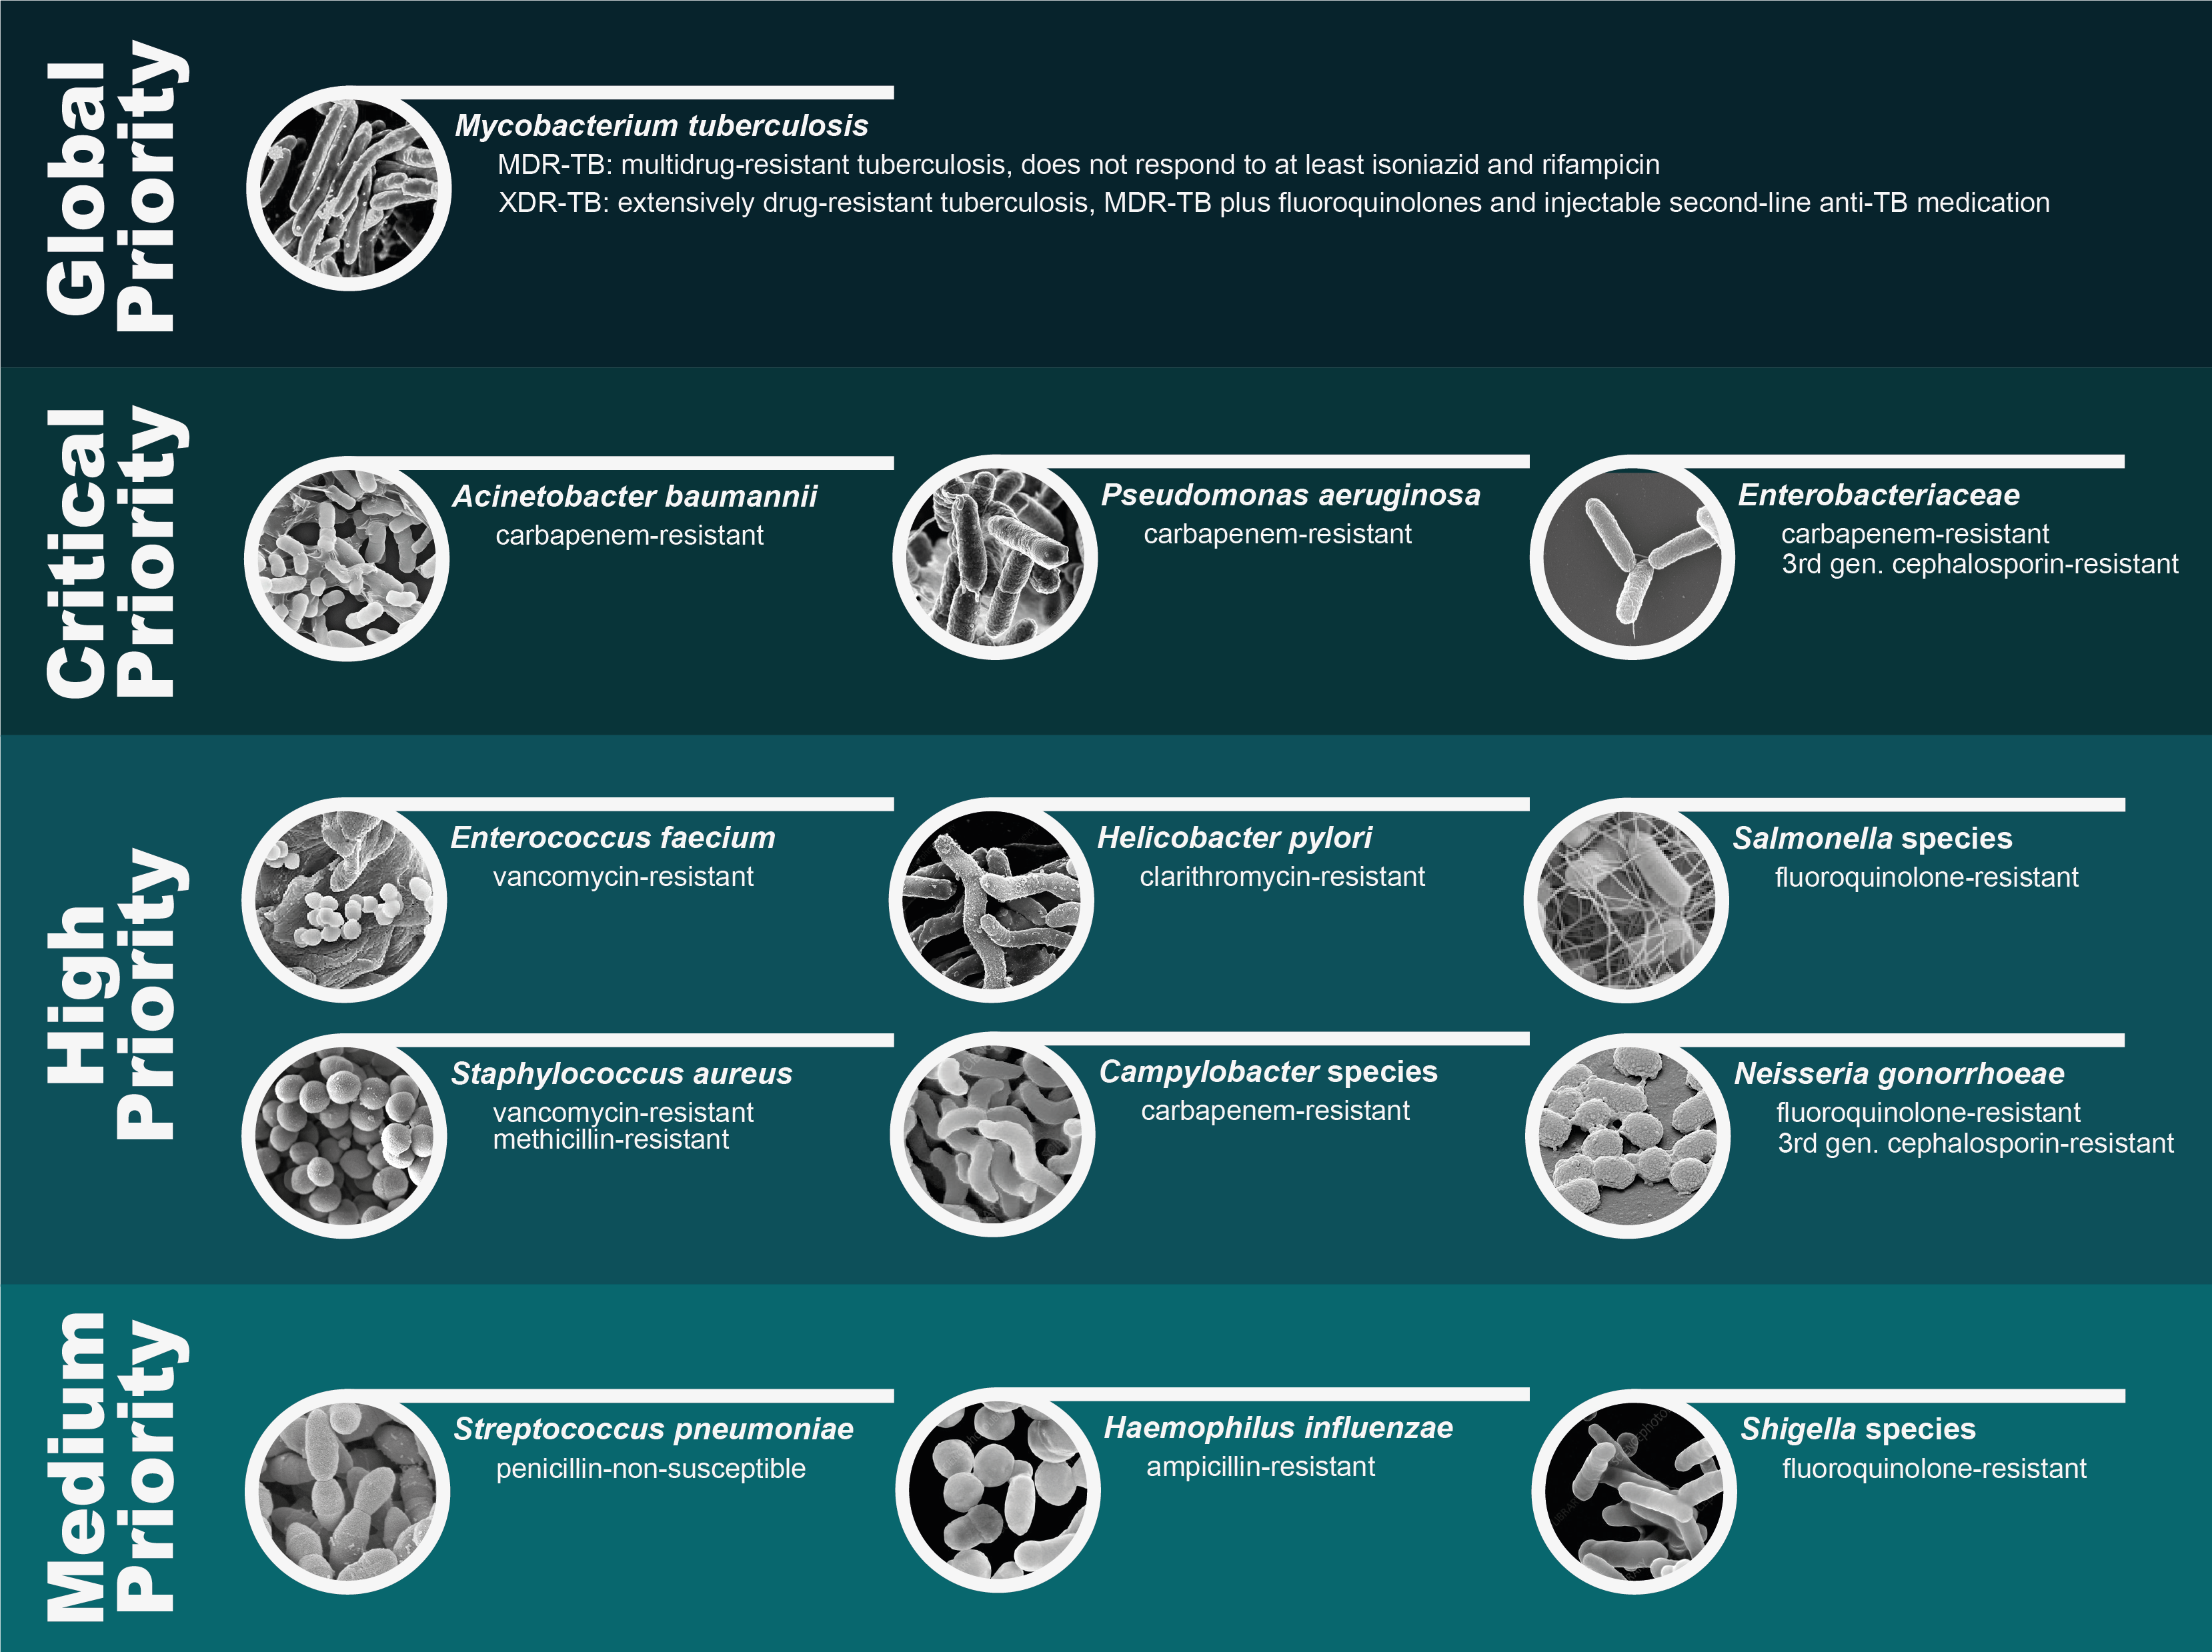
\includegraphics[width=\textwidth]{figures/introduction/Figure 1.pdf}
\caption{\textbf{World Health Organisation Global Priority Pathogens list.} This catalogue includes, besides \textit{Mycobacterium tuberculosis} considered the number one global priority, a list of twelve microorganisms grouped under three priority tiers according to their antimicrobial resistance: critical (\textit{Acinetobacter baumannii}, \textit{Pseudomonas aeruginosa} and \textit{Enterobacteriaceae}), high (\textit{Enterococcus faecium}, \textit{Helicobacter pylori}, \textit{Salmonella} species, \textit{Staphylococcus aureus}, \textit{Campylobacter} species and \textit{Neisseria gonorrhoeae}), and medium (\textit{Streptococcus pneumoniae}, \textit{Haemophilus influenzae} and \textit{Shigella} species). The major objective was to encourage the prioritisation of funding and incentives, align research and development priorities of public health relevance, and garner global coordination in the fight against antimicrobial resistant bacteria. Adapted from \cite{world_health_organization_prioritization_2017}.}
\label{fig:figure1}
\end{figure*}

Clinical microbiology is a discipline focused on rapidly characterising pathogen samples to direct the management of individual infected patients (diagnostic microbiology) and monitor the epidemiology of infectious disease (public health microbiology), including the detection of outbreaks and infection prevention. 
According to the \ac{WHO} Global Health Spending Report from 2000 to 2019, of the 51 countries that reported health spending by disease and condition, an average of 37\% of health spending went to infectious and parasitic diseases, corresponding to the largest share of health spending \citep{world_health_organization_global_2021}. 
About 21\% of total health spending went to three major infectious diseases - HIV / AIDS (9\%), tuberculosis (1\%) and malaria (11\%) - and 16\% went to other infectious and parasitic diseases. 
On average, 70\% of external health aid went to infectious and parasitic diseases in 51 low- and middle-income countries. 
Of the \$54.8 billion estimated disbursed for health in 2020, \$13.7 billion (25\%) was targeted toward the COVID-19 health response \citep{micah_tracking_2021}.

\subsection{Current standards for diagnostic in clinical microbiology} \label{ssec:_intro_current_standards}

The past few decades have seen a major revolution in the operation of microbial laboratories, driven by the development of molecular technologies and ways to make these accessible, namely amplification-based \ac{PCR}, matrix-assisted laser desorption/ionisation - time of flight (MALDI-TOF) and DNA-microarray-based hybridisation technology. 
These are used in conjunction with traditional techniques such as microscopy, culture, and serology.
Application of these methods differs by suspected infection type: bacterial, viral, fungal or parasitic. 
For the purpose of this dissertation work, we will focus on bacterial (see Section \ref{sssec:_intro_bacterial} and viral infections (see Section \ref{sssec:_intro_viral}.

\subsubsection{Bacterial infections} \label{sssec:_intro_bacterial}

For patients with bacterial infections, the crucial steps are (1) to grow an isolate from a specimen, (2) identify its species, and (3) determine its pathogenic potential and test its susceptibility to antimicrobial drugs  \citep{didelot_transforming_2012}. 
Together, this information facilitates the specific and rational treatment of patients. 
For public health purposes, knowledge also needs to be gained about (4) the relatedness of the pathogen to other strains of the same species to investigate transmission routes and allow recognition of outbreaks \citep{foxman_choosing_2005} (see Figure \ref{fig:figure2}). 

\begin{figure*}[h!]
\centering
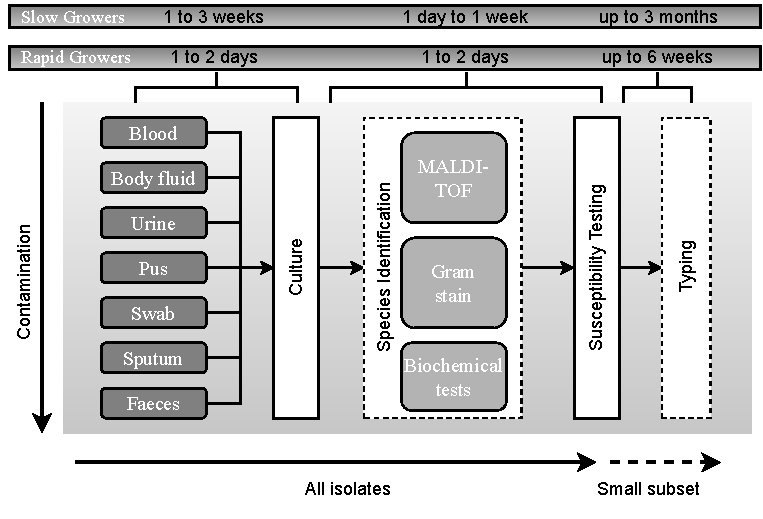
\includegraphics[width=\textwidth]{figures/introduction/Figure 2.pdf}
\caption{\textbf{Principles of current processing of bacterial pathogens.} Schematic representation of the current workflow for processing samples for bacterial pathogens is presented, with high complexity and a typical timescale of a few weeks to a few months. Samples that are likely to be normally sterile are often cultured on rich medium that will support the grown of any culturable organism. Samples contaminated with colonising flora present a challenge for growing the infecting pathogen. Many types of culture media (referred to as selective media) are used to favour the growth of the suspected pathogen.
Once an organism is growing, the likely pathogens are then processed through a complex pathway that has many contingencies to determine species and antimicrobial susceptibility. Broadly, there are two approaches. One approach uses MALDI-TOF for species identification prior to setting up susceptibility testing. The other uses Gram staining followed by biochemical testing to determine species; susceptibility testing is often set up simultaneously with doing biochemical tests. Lastly, depending on the species and perceived likelihood of an outbreak, a small subset of isolates may be chosen for further investigation using a wide range of typing tests. Adapted from \cite{didelot_transforming_2012}.}
\label{fig:figure2}
\end{figure*}

The current gold standard for bacterial pathogen identification in diagnostic microbiology laboratories involves the isolation of the pathogen through culture followed by biochemical testing, a multi-step process that can take days to weeks before obtaining results, depending on the fastidiousness of the organism and if it can be cultured \citep{muhamad_rizal_advantages_2020, giuliano_guide_2019, muhamad_rizal_advantages_2020}. 
Although culture allows the identification of a wide variety of organisms, some pathogens can escape routine investigation due to strict metabolic necessities for growth or the requirement for specific biochemical tests needed for their identification. 
Furthermore, results will be obscured if a mixed culture is obtained, particularly if the cultures are obtained from sites with a microbiota, such as the gut and the skin, increasing the risk of contamination by normal flora and leading to false results \citep{giuliano_guide_2019}. 
After successful growth in culture, Gram staining and MALDI-TOF mass spectrometry are often used for identification with good accuracy as long as the pathogen is presented in the the coexisting database \citep{patel_maldi-tof_2015}. 
An alternate rapid identification method is \ac{PCR} where nucleic acid fragments are detected through specific primers, being highly sensitive and specific, to the point where \ac{PCR} may detect bacteria that are not viable after a patient has been treated for an infection and it is limited to the primer used \citep{scerbo_beyond_2016}. 
Syndromic panels, an extension of \ac{PCR} by using multiple primers (multiplex \ac{PCR}) to simultaneously amplify nucleic acids from multiple targets in a single reaction, tried to address this issue by allowing for the identification of multiple bacteria and other important information such as the detection of antibiotic resistance or virulence genes \citep{giuliano_guide_2019}.

Following identification, antibiotic-susceptibility testing is essential to guide clinicians in selecting an appropriate treatment. 
Conventional methods of bacterial resistance detection, such as disc diffusion, antimicrobial gradient strip, and broth microdilution, are widely used, but results cannot be obtained before 48 hours after receiving a sample, which can lead to prolonged use or overuse of broad-spectrum antibiotics \citep{benkova_antimicrobial_2020}. 
Similarly to bacterial identification, MALDI-TOF and \ac{PCR} have been increasingly adopted as solutions with shorter turnaround times, although no phenotypic information is recovered, nor information on the minimum inhibitory concentration (MIC) for a given antibiotic.   

Choosing an appropriate bacterial typing technique for epidemiological studies depends on the available resources and the minimum intended resolution, ranging from DNA fingerprinting to multilocus sequence typing, \ac{PFGE}, and sequence-based typing (see \secref{sec:_intro_genomics_approach}) \citep{allerberger_molecular_2012,foxman_choosing_2005}. 
DNA macrorestriction analysis by \ac{PFGE}, which revolutionised precise separation of DNA fragments, became the most widely implemented DNA fingerprinting technique \citep{allerberger_molecular_2012}, becoming the golden standard for bacterial typing \citep{neoh_pulsed-field_2019}.

In the early 2000s, \ac{MLST} was proposed as a portable, universal, and definitive method for characterising bacteria \citep{maiden_multilocus_2006}. 
Instead of enzyme restriction of bacteria DNA, separation of restricted DNA bands using a \ac{PFGE} chamber, followed by clonal assignment of bacteria based on banding patterns, \ac{MLST} relies on the amplification through \ac{PCR} sequences of internal fragments of housekeeping genes (usually 5 to 7), approximately 450-500 \ac{bp} in size, followed by its sequence, usually my Sanger methods (see \secref{ssec:_intro_1st_gen_seq}). 
For each house-keeping gene, the different sequences present within a bacterial species are assigned as distinct alleles and, for each isolate, the alleles at each of the (usually) seven loci define the allelic profile or sequence type \citep{larsen_multilocus_2012}. 
As with \ac{PFGE}, different schemes, defining what housekeeping gene fragments are used, are available depending on the species. 
Unlike \ac{PFGE}, the provision of freely accessible, curated databases of \ac{MLST} nucleotide sequence data enables the direct comparison of bacterial isolates, providing the basis of a common language for bacterial typing \citep{maiden_multilocus_2006}. 
So far, \ac{MLST} schemes for more than 100 bacterial organisms have been published and made freely available\footnote{\url{https://pubmlst.org/organisms}}, \cite{jolley_open-access_2018}) 

Depending on the organism identified, further and/or particular typing schemes can be applied. 
For \textit{S. pneumoniae}, one of the pathogens listed in the \ac{WHO} \ac{GPP} list, the typing of the polysaccharide capsule, usually through Quellung reaction, is paramount for disease surveillance and evaluation of the pre- and post-pneumococcal vaccine, since the capsule, with over 90 serotypes reported, is the dominant surface structure of the organism and plays a critical role in virulence \citep{jauneikaite_current_2015, paton_streptococcus_2019}. 
For the \textit{Salmonella} species, also in the \ac{GPP} list, the serotype is usually determined by agglutination of the bacteria with specific antisera to identify variants of somatic (O) and flagella (H) antigens that, in various combinations, characterise more than 2600 reported serotypes \citep{diep_salmonella_2019}. 

\subsubsection{Viral infections} \label{sssec:_intro_viral}

Traditional approaches to laboratory diagnosis of viral infections have been (1) direct detection in patient material of virions, viral antigens, or viral nucleic acids, (2) isolation of the virus in cultured cells, followed by identification of the isolate, and (3) detection and measurement of antibodies in patient serum (serology) \citep{burrell_laboratory_2017}. 
Viral diagnostics is therefore generally organised into two primary categories, indirect and direct detection, depending on the method used. 

Indirect detection methods involve the propagation of virus particles through their introduction to a suitable host cell line (virus isolation), since viruses rely on host organisms to replicate. 
This is a relatively slow diagnostic method, sometimes taking weeks for the virus to propagate, usually followed by microscopy for its identification, or more commonly, through molecular methods with an agent that detects a virus-associated protein, such as an antibody \citep{cassedy_virus_2021}. 

Direct detection methods negate the need for virus propagation, detecting the virus directly from the suspect source through nucleic acid and immunological methods. 
\ac{PCR} and reverse transcription-PCR (RT-PCR) are widely applied methods for the detection of both DNA and RNA viruses, respectively, driven by increased awareness of the clinical value of and demand for prompt information about viral loads, viral sequence data and potential antiviral resistance information \citep{cassedy_virus_2021}. 
Syndromic testing (see \secref{sssec:_intro_bacterial}) is now fully integrated into standard testing practises of many clinical laboratories \citep{dien_bard_panels_2020}. 
The limitations of these assays include the absence of detection of off-target pathogens, a lack of full susceptibility information, cost, and false positive results. 
\ac{qPCR} remains the front line tool in aetiological diagnosis, measuring the production of the target amplicon throughout the reaction and providing quantitative results with high specificity and sensibility, albeit with a significant cost due to sophisticated apparatus despite high-throughput systems being widely established \citep{cassedy_virus_2021}.

Immunoassays employ singular-epitope specificity antibodies as the primary means to detect viruses within a sample and provide a much more cost-efficient alternative to nucleic acid detection \citep{cassedy_virus_2021}. 
A major application is seroprevalence assays, an essential technique to identify patients who have been exposed to a virus (historical exposure), detect asymptomatic infection, or evaluate the efficacy of vaccines \citep{chan_determining_2021, bobrovitz_global_2021}. 
\ac{LFIA} are widely used to detect virus-associated proteins directly from the source through antibodies labelled that binding to their cognate antigens, usually read by means of a colour change at a test line. 
In addition to being very cost-effective, \ac{LFIA} have a turnaround time of minutes and the colour change can be observed with the naked eye, therefore facilitating rapid diagnosis, but their results are limited to semiquantitative and typically do not achieve sensitivity comparable to nucleic acid detection \citep{estrela_lateral_2016, cassedy_virus_2021, di_nardo_ten_2021}.

\subsection{Surveillance and infection prevention in public health} \label{ssec:_intro_survaillance}

Infectious disease surveillance is critical for improving population health, generating information that drives action not only in the management of infected patients but also in the prevention of new ones by identifying emerging health conditions that may have a significant impact by (1) describing the current burden and epidemiology of the disease, (2) to monitoring trends, and (3) identifying outbreaks and new pathogens \citep{groseclose_public_2017, murray_infectious_2017}. 
\ac{PHSS} consist of the ongoing systematic collection, analysis and interpretation of data, and its integration with the timely dissemination of results to those who can carry out effective prevention and control activities \citep{teutsch_considerations_2010}. 

Traditional \ac{PHSS} can have different approaches based on the epidemiology and clinical presentation of the disease and the goals of surveillance. 
In passive surveillance systems, medical professionals in the community and health facilities report cases to the public health agency, which conducts data management and analysis once the data is received and communicates with the responsible entities. 
Globally, the \ac{WHO} as described in the International Health Regulations what is notifiable by all countries, such as severe acute respiratory syndrome (SARS) and viral hemorrhagic fevers (Ebola, Lassa, Marburg), as well as guiding which public health measures should be implemented \citep{world_health_organization_international_2005}. 
Active surveillance aims to detect every case, not relying on a reporting structure, and can have many approaches from sentinel sites or network of sites that capture cases of a given condition, such as respiratory tract infections, within a catchment population \citep{murray_infectious_2017, melo-cristino_estudo_2006}. 
The application of environmental surveillance methods, performed prospectively to detect pathogens prior to the recording of clinical cases or to monitor their abundance in the environment to assess the potential risk of disease, has been proven as a viable alternative, particularly in wastewater \citep{andrews_environmental_2020, mcweeney_demonstration_1894, baker_combined_2011, larsen_tracking_2020}.  

The emergence and reemergence of infectious diseases are closely linked to the biology and ecology of infectious agents, their hosts, and their vectors \citep{destoumieux-garzon_one_2018}.
"One Health" is a collaborative and multi-disciplinary approach to designing and implementing programmes, policies, legislation and research in which multiple sectors communicate and work together to achieve better public health outcomes \citep{mackenzie_one_2019}. 
It recognises that people's health is closely related to the health of animals and the shared environment, focussing on zoonotic and vector-borne diseases, antimicrobial resistance, food safety, food security, and environmental contamination \citep{rugarabamu_one-health_2021}.
This is crucial to (1) understanding the emergence and re-emergence of infectious and noncommunicable chronic diseases and (2) in creating innovative control strategies.
A better understanding of the causes and consequences of certain human activities, lifestyles, and behaviours in ecosystems is crucial for a rigorous interpretation of disease dynamics and to drive public policies, but it requires breaking down the interdisciplinary barriers that still separate human and veterinary medicine from ecological, evolutionary, and environmental sciences \citep{destoumieux-garzon_one_2018}. 

\section{A genomic approach to clinical microbiology} \label{sec:_intro_genomics_approach}

Since the publication of the first complete microbial genome, a quarter of a century ago, of the bacterium \textit{Haemophilus influenzae} \citep{hood_dna_1996}, genomics has transformed the field of microbiology, and in particular its clinical application (see Figure \ref{fig:figure3}). 

\begin{figure*}[h!]
\centering
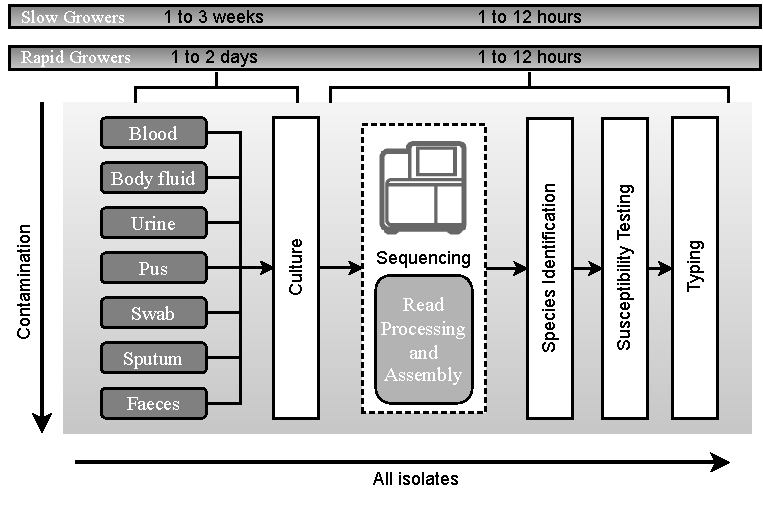
\includegraphics[width=\textwidth]{figures/introduction/Figure 3.pdf}
\caption{\textbf{Principles of current processing of bacterial pathogens based on whole genome sequencing.} Schematic representation of the workflow for processing samples for bacterial pathogens after the adoption of whole genome sequencing, with an expected timescale that could fit within a single day. The culture steps would be the same as currently used in a routine microbiology laboratory (see Figure \ref{fig:figure2}). Once a likely pathogen is ready for sequencing, DNA is extracted, taking as little as 2 hours to prepare the DNA for sequencing.
After sequencing, the main processes for yielding information is computational. Automated sequence assembly algorithms are necessary for processing the raw sequence data, from which species, relationship to other isolates of the same species, antimicrobial resistance profile and virulence gene content can be assessed. All the results can also be used for outbreak detection and infectious diseases surveillance. Adapted from \cite{didelot_transforming_2012}}
\label{fig:figure3}
\end{figure*}

The paper describing the DNA-sequencing method with chain-terminating inhibitors used in the sequencing of the first microbial genome \citep{sanger_dna_1977}, which earned the late Frederick Sanger his share of the 1980 Nobel Prize in Chemistry alongside Walter Gilbert, was, in 2014, the top fourth in the number of citations with over 60000, highlighting its impact in the field of biological sciences, and by extension medicine \citep{van_noorden_top_2014}. 
Currently, this number has increased to over 84000 according to \ac{PMC}\footnote{\url{https://pubmed.ncbi.nlm.nih.gov/}}\footnote{\url{ https://www.ncbi.nlm.nih.gov/pmc/articles/PMC431765/}}. 
Since its emergence, reductions in cost, technical advances in sequencing technologies, and new computational developments have made genomic sequencing one of the most influential tools in biomedical research, yielding unprecedented insights into microbial evolution and diversity, and the complexity of the genetic variation in both commensal and pathogenic microbes. 
The emerging application of genomic technologies in the clinic to combat infectious diseases is transforming clinical diagnostics and the detection and surveillance of outbreaks. 

\subsection{Twenty five years of microbial genome sequencing} \label{ssec:_intro_sequencing}

Since the discovery of the structure of DNA \citep{watson_molecular_1953}, great strides have been made in understanding the complexity and diversity of genomes in health and disease. 
The development and commercialisation of high-throughput, massively parallel sequencing has democratised sequencing by offering individual laboratories, either in research or in health, access to the technology. 
Over the last quarter of a century, three main revolutions can be considered in genomic sequencing: the first, the second and the third generations of sequencing (see Figure ~\ref{fig:figure5}).

\begin{figure*}[h!]
\centering
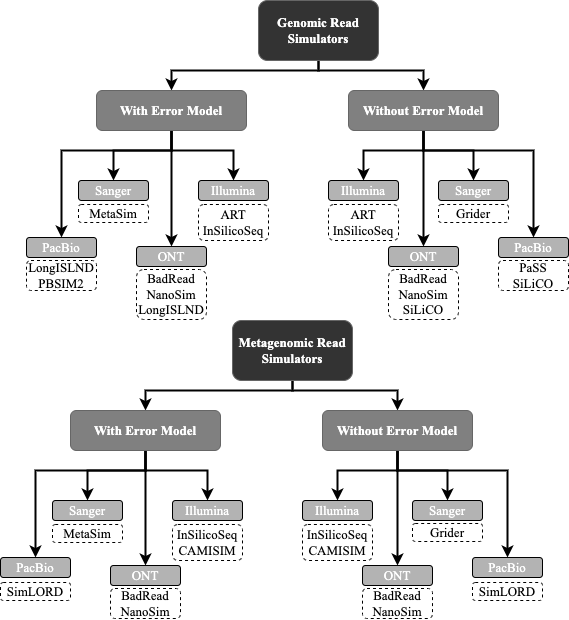
\includegraphics[width=\textwidth]{figures/introduction/Figure 5.png}
\caption{\textbf{The three revolutions in sequencing technology that have transformed the landscape of bacterial genome sequencing.} The first-generation, also known as Sanger sequencers, is represented by the ABI Capillary Sequencer (Applied Biosystems). During the sequencing reaction, at each nucleotide incorporation event, a fluorescently labelled \ac{ddNTP} is incorporated, terminating the elongation of the DNA molecule. The resulting electropherogram for sequencing reaction is below, and is read from left to right. The second-generation, also known as high-throughput sequencers, is represented by MiSeq, a 4-channel sequencer, and NextSeq, a 2-channel sequencer (Illumina), both sequencing by synthesis instruments. For both instruments, the loaded flowcell is sequenced in massive parallel reactions, with each nucleotide incorporation emitting a light signal that is captured and latter basecalled into a fastq file, with indication of the confidence of the call, presented below. In a 4-channel instrument each nucleotide has its own marker (A: yellow, T: green, C: red, G: blue) but in a 2-channel instrument only 2 markers exist (A: green plus red, T: green, C: red, G: no marker). These instruments allow the sequencing of both ends of the DNA fragment. Lastly, the third-generation, also known as long-read sequencers, is represented by the Pacific Bioscience BS sequencer and Oxford Nanopore MinION sequencer. In the first, immobilised polymerases in a SMRT Cell incorporating nucleotides with identifying fluorescent labels. In the latter, a nanopore embedded in a solid-state membrane causes a change in an ionic current across the membrane each time a nucleotide is pushed through the pore. This difference in potential is then used for basecalling. Adapted from \cite{hagemann_overview_2015, loman_twenty_2015,goodwin_coming_2016, wang_nanopore_2021, metzker_sequencing_2010, xu_recent_2020}}
\label{fig:figure5}
\end{figure*}

\subsubsection{The first-generation of DNA sequencing} \label{ssec:_intro_1st_gen_seq}

In the late 1980s, automated Sanger sequencing machines could sequence approximately 1,000 bases per day, having been applied in the 1990s to large bacterial genomes and the first unicellular and multicellular eukaryotic genomes \citep{koch_sequencing_2021}. 
The first genomes of pathogenic \textit{Mycobacterium tuberculosis} \citep{cole_deciphering_1998}, \textit{Yersinia pestis} \citep{parkhill_genome_2001}, \textit{Escherichia coli} K-12 \citep{blattner_complete_1997} were sequenced using this technology, requiring years of effort and significant budgets, but providing insights into the genomic complexity of these organisms. 
Some of the complete genome sequences produced during this era are still used today as high-quality references. 

Simplistically, in first-generation DNA sequencing, also known as Sanger sequencing, a DNA polymerase is used to synthesise numerous copies of the sequence of interest using \ac{ddNTP}) in the reaction. 
At each nucleotide incorporation event, there is a chance that a \ac{ddNTP} will be added and the growing DNA chain will terminate, resulting in a collection of DNA molecules of varying lengths \citep{sanger_dna_1977, hagemann_overview_2015}. 
Modern Sanger sequencing uses fluorescently labelled \ac{ddNTP} that allow the amplification step to be performed in a single reaction, resulting in a mixture of single-stranded DNA fragments of various lengths, each tagged at one end with a fluorophore indicating the identity of the 3' nucleotide that, after separation through capillary electrophoresis, the resulting electropherogram with four-colour fluorescence intensity can be interpreted by a base-calling software and producing 600–1000 bases of accurate sequence per reaction\citep{hagemann_overview_2015}. 

The first generation sequencing technology remains very useful for applications where high-throughput is not required due to its cost-effectiveness, relatively low sample load and accuracy of sequencing, even in repetitive genomic regions, although input DNA must consist of a relatively pure population of sequences \citep{slatko_overview_2018}. 
One of the most common uses is thus individual sequencing reactions using a specific DNA primer on a specific template, such as \ac{MLST} of bacterial genomes. 

\subsubsection{The second-generation of DNA sequencing} \label{ssec:_intro_2nd_gen_seq}

The release of the first truly high-throughput sequencing platform in the mid-2000s heralded a 50,000-fold drop in the cost of DNA sequencing in comparison with the first-generation technologies and led to the denomination of the second generation as next-generation sequencing (NGS) \citep{goodwin_coming_2016}. 
This trend has continued over the next two decades of continued development and improvement, allied to the emergence of benchtop sequencing platforms with a high-throughput sequencing data and turnaround times of days, making it a standard in any microbiology and public health laboratories \citep{loman_twenty_2015}. 
Second-generation sequencing methods can be grouped into two major categories: (1) sequencing by hybridisation and (2) sequencing by synthesis. 

\paragraph{Sequencing by hybridisation} \label{sssec:_intro_2nd_gen_seq_hybrid} \mbox{}\\

Sequencing by hybridisation, also known as sequencing by ligation, originally developed in the 1980s, relies on the binding of one strand of DNA to its complementary strand (hybridisation). 
By repeated hybridisation and washing cycles, it was possible to build larger contiguous sequence information, based on overlapping information from the probe hybridisation spot, being sensitive to even single-base mismatches when the hybrid region is short or if specialised mismatch detection proteins are present \citep{slatko_overview_2018, detter_nucleic_2014}. 
Although widely implemented via DNA chips or microarrays, has largely been displaced by other methods, including sequencing by synthesis \citep{goodwin_coming_2016}. 

\paragraph{Sequencing by synthesis} \label{sssec:_intro_2nd_gen_seq_synth} \mbox{}\\

Sequencing by synthesis methods is a further development of Sanger sequencing, without the \ac{ddNTP} terminators, in combination with repeated cycles, run in parallel, of synthesis, imaging, and methods to incorporate additional nucleotides in the growing chain. 
All second-generation sequencing by synthesis approaches relies on a ‘library’ preparation using native or amplified DNA usually obtained by (1) DNA extraction, (2) DNA fragmentation and fragment size selection, and (3) ligation of adapters and optional barcodes to the ends of each fragment. 
This is generally followed by a step of DNA amplification. The resulting library is (4) loaded into a flow cell and (5) sequenced in massive parallel sequencing reactions \citep{giani_long_2020}.
Besides having much shorter read lengths than first-generation methods, with reads ranging from 45 to 300 bases,. These have an intrinsically higher error rate, the massively parallel sequencing of millions to billions of short DNA sequence reads allows the obtainment of millions of accurate sequences based on the identification of consensus (agreement) sequences \citep{slatko_overview_2018, goodwin_coming_2016, hagemann_overview_2015}. 

Many of the approaches currently available for sequencing by synthesis methods have been described as cyclic array sequencing platforms, as they involve dispersal of target sequences across the surface of a two-dimensional array, followed by sequencing of those targets \citep{hagemann_overview_2015}. 
They can also be classified as single nucleotide addition or cyclic reversible termination or as single nucleotide addition \citep{goodwin_coming_2016}. 

The first relies on a single signal to mark the incorporation of a \ac{dNTP} into an elongating strand, avoiding the use of terminators. 
As a consequence, each of the four nucleotides must be added iteratively to a sequencing reaction to ensure that only one \ac{dNTP} is responsible for the signal. 
The Roche 454 Life Sciences pyrosequencing device \footnote{\url{https://web.archive.org/web/20161226040638/http://454.com/}, snapshot from 26 December 2016}, was the first and most popular instrument implementing this technology, but discontinued since 2013 with support to the platform ceasing in 2016. 
This system distributes template-bound beads into a PicoTiterPlate along with beads containing an enzyme cocktail. 
As a \ac{dNTP} is incorporated into a strand, an enzymatic cascade occurs, resulting in a bio-luminescence signal which is captured by a camera, which can be attributed to the incorporation of one or more identical \ac{dNTP}s at a particular bead \citep{goodwin_coming_2016}. 
The ThermoFisher Ion Torrent system \footnote{\url{https://www.thermofisher.com/pt/en/home/brands/ion-torrent.html}}, released in 2010 and still available today, replaces the optical sensor, using instead  H+ ions that are released as each \ac{dNTP} is incorporated in the enzymatic cascade, and the consequential change in pH, to detect a signal \citep{goodwin_coming_2016}. 
Alongside the 454 pyrosequencing system, this system has difficulty in enumerating long repeats, additionally, the throughput of the method depends on the number of wells per chip, ranging from 10 megabases to 1000 megabases of 100 base reads in length, but with a very short run time (three hours) \citep{hagemann_overview_2015, loman_performance_2012}.

The latter is defined by their use of terminator molecules that are similar to those used in the first-generation of sequencing, preventing elongation of the DNA molecule, but unlike the first methods, it is reversible. 
To begin the process, a DNA template is primed by a sequence that is complementary to an adapter region, which will initiate polymerase binding to this double-stranded DNA region. 
During each cycle, a mixture of all four individually labelled and 3'-blocked \ac{dNTP}s are added. 
After incorporation of a single \ac{dNTP} into each elongating complementary strand, the unbound \ac{dNTP}s are removed and the surface is imaged to identify which \ac{dNTP} was incorporated at each cluster by optical capture. 
The fluorophore and blocking group can then be removed and a new cycle can begin \citep{goodwin_coming_2016}. 
The Illumina systems, which use this technology, accounts for the largest market share for sequencing instruments compared to other platforms\footnote{\url{https://www.forbes.com/companies/illumina/?sh=774358a91aa6}}, allowing paired-end sequencing and having the highest throughput (from 25 million reads for a MiSeq instrument to  1.2 billion reads for a NextSeq instrument\footnote{\url{https://www.illumina.com/systems/sequencing-platforms.html}}), with read lengths ranging from 45 to 300 bases in length with high accuracy, albeit with long running times (4 to 55 hours), rendering this technology a good choice for many sequencing applications where large read length is not required \citep{loman_performance_2012, gupta_chapter_2014, hagemann_overview_2015}.

\subsubsection{The third-generation of DNA sequencing} \label{ssec:_intro_3rd_gen_seq}

Despite their wide adoption, second-generation methods require in the library preparation an enrichment or amplification step. 
These steps are time-consuming, introduce biases related to preferential capture or amplification of certain regions, and produce reads with relatively small size, making transversing repetitive genomic regions impossible if they are larger than the read length \citep{hagemann_overview_2015}. 
Third-generation sequencing technologies, also known as long-read sequencing or single-molecule sequencing, are characterised by the generation of ultra-long-reads, albeit at a much lower throughput than the second-generation \citep{hoang_long-reads-based_2022}. 
They also have the potential to go beyond four-base sequencing to reveal genome-wide patterns of methylation and other chemical modifications that control the biology or the virulence of pathogens \citep{korlach_going_2012}. 
Currently, commercial long-read sequencing is supported by two companies: Pacific Biosciences\footnote{\url{https://www.pacb.com/}} and Oxford Nanopore Technologies\footnote{\url{https://nanoporetech.com/}}. 

The basis of Pacific Biosciences sequencers is known as single-molecule real-time sequencing (SMRT), which takes place in single-use SMRT Cells. 
These contain multiple immobilised polymerases, which, after binding to an adaptor sequence, begin replication incorporating nucleotides with identifying fluorescent labels. 
The sequence of fluorescence pulses is recorded into a movie which is then converted into a nucleotide sequence. 
After the polymerase completes replication of one DNA strand, it continues to sequence the opposite adapter and second strand. 
As a result, multiple passes of the same template can be generated depending on the lifetime of the polymerase \citep{hoang_long-reads-based_2022, loman_twenty_2015}. 
This technology has accuracy comparable with the Illumina systems but requires a higher initial investment cost, are much larger machines in comparison with the benchtop counterparts, and have much lower throughput and longer library preparation protocols \citep{hoang_long-reads-based_2022, wenger_accurate_2019}. 

Oxford Nanopore Technologies makes use of nanopores in small, portable single-molecule sequencing devices, capable of generating ultra-long sequences in real-time at a relatively low cost. 
Biological nanopores are embedded in solid-state membranes within disposable flow cells which, when a DNA strand passes through the pore driven by a motor protein, each nucleotide causes a change in an ionic current across the membrane, which is later base called \citep{hoang_long-reads-based_2022, loman_twenty_2015}. 
This process is free from fluorescence labels and amplification requirements, and after one strand is processed, the pore is available to sequence the next available strand. 
Sequence quality and length depend on the loaded library but are usually much lower than the alternative counterparts, and its throughput is dependent on the number and lifespan of the nanopore within the flowcell, but still much lower than the alternatives. 
Despite this, its portability, fast advances, and continued improvement of the flowcells make this a fast adopted technology for long-read sequencing.  

\subsection{DNA sequencing in clinical diagnosis and surveillance} \label{ssec:_intro_sequencing_diagnosis}

Whole-genome sequencing (WGS) is becoming one of the most widely used applications of microbial genome sequencing. 
The major advantage of WGS is to yield all the available DNA information content on isolates in a single rapid step following culture (sequencing without culture will be discussed in the \secref{ssec:_intro_metagenomics}). 
In principle, after obtaining a pure culture, either bacterial (see \secref{sssec:_intro_bacterial}) or viral (see \secref{sssec:_intro_viral}), the data from sequencing contain all the information currently used for diagnostic and typing needs, and much more, thus opening the prospect for large-scale research into pathogen genotype-phenotype associations from routinely collected data \citep{didelot_transforming_2012}.
The cost of producing massive amounts of information requires a new framework with expert handling and processing of computer-driven genomic information, as well as capable computational infrastructures (see Section \ref{sec:_intro_bioinformatics}), but through this technology, researchers and clinicians can obtain the most comprehensive view of genomic information and associated biological implications, transforming clinical diagnostics and the detection and surveillance of outbreaks. \citep{cirulli_uncovering_2010, nature_reviews_genetics_genomic_2019, goodwin_coming_2016}.

Targeted sequencing is also proving invaluable to clinical microbial and research, not only by allowing more individual samples to be sequenced within a single run, significantly reducing costs and the amount of data generated, but also, due to the smaller target size, obtaining results with very high confidence due to the high coverage obtained \citep{goodwin_coming_2016}.
This has been particularly useful in viral genomics where sections, such as the capsid, or the complete viral genome can be selectively targeted directly from the suspected sample, offering a more time-effective method to achieve the same output as traditional nucleic acid amplification methods \citep{cassedy_virus_2021}. 

\subsubsection{Sequencing in the routine laboratory workflow} \label{sssec:_intro_sequencing_routine_lab}

WGS has been used in the routine laboratory workflow when typing of pathogens by a method having the highest possible discriminatory power is required either through single nucleotide polymorphism (SNP) or core-genome/whole genome MLST (cg/wg MLST) analysis, for example during hospital outbreaks \citep{tagini_bacterial_2017}. 

The implementation of WGS in routine diagnostics requires several adaptations in the laboratory workflow, from the ‘wet’ laboratory part (extraction, library preparation, sequencing), to the ‘dry’ bioinformatics part where genomic data is analysed and its results interpreted by specialised personnel \citep{rossen_practical_2018}. 

Currently, sequencing technologies are used in a case-by-case approach, with its adoption being much more present in a research setting than in a diagnostic one. 
Sequencing is mostly used after a diagnostic through the identification of the causative agent has already been performed. 
Although substantial advances have been made in reducing response time, most of the current systems do not yet generate enough data fast enough for a truly rapid response for it to be used in the clinical setting \citep{goodwin_coming_2016}. 
High-throughput DNA sequencing has found additional new applications in drug discovery and in functional genomics with, for example, SNP-based analysis to identify new drug targets \citep{loman_twenty_2015}.

Although the second-generation DNA sequencing methods have shed light on fundamental aspects of microbial ecology and function, they suffer from issues associated with short read length (see \ref{ssec:_intro_2nd_gen_seq}) and cannot reliably reconstruct long repeats because of uncertainties in mapping read, even when paired-end sequencing is used. 
Third-generation sequencing methods (see \ref{ssec:_intro_3rd_gen_seq}) have become increasingly used in microbiology, although their accuracy and low throughput make it challenging to implement in a clinical diagnostic setting. 

\subsubsection{Sequencing and genomic surveillance} \label{sssec:_intro_sequencing_genomic_survaillance}

Most notably, WGS has become a common tool in surveillance and infection prevention, allowing for pathogen identification and tracking, establishing transmission routes and outbreak control \citep{lo_genomics_2020}. 
In bacterial infections, initiatives such as Pathogenwatch\footnote{\url{https://pathogen.watch/}} offers a web-based platform for \ac{AMR} analysis and phylogeny generation of \textit{Campylobacter}, \textit{Klebsiella}, \textit{Neisseria gonorrhoeae}, \textit{Staphylococcus aureus}, and \textit{Salmonella Typhi} \citep{afolayan_overcoming_2021}. 
The Center for Genomic Epidemiology website\footnote{\url{https://www.genomicepidemiology.org/}} offers services for phylogenetic tree building and \ac{AMR} prediction. 
Chewie Nomenclature Server\footnote{\url{https://chewbbaca.online/}} allows users to share genome-based gene-by-gene typing schemas and to maintain a common nomenclature, simplifying the comparison of results \citep{mamede_chewie_2021}. 
Enterobase\footnote{\url{https://enterobase.warwick.ac.uk/}} allows for the analysis and visualisation of genomic variation within enteric bacteria \citep{zhou_enterobase_2020}. 
Microreact\footnote{\url{https://microreact.org/}}, from the same developers as Pathogenwatch, combines clustering, geographical and temporal data into an interactive visualisation with trees, maps, timelines and tables for a multitude of microorganisms, both bacterial and viral \citep{argimon_microreact_nodate}. 
Particularly for viruses, GISAID\footnote{\url{https://www.gisaid.org/}}  promotes the rapid sharing of data from all influenza viruses and the coronavirus causing COVID-19, including the genetic sequences and related clinical and epidemiological data \citep{shu_gisaid_2017}. 
ViPR\footnote{\url{https://www.viprbrc.org/}} provides access to sequence records, gene and protein annotations, immune epitopes, 3D structures, host factor data, and other data types for over 14 viral families, including \textit{Coronaviridae}, from which \ac{SARS-CoV-2} belongs to, and \textit{Faviviridae}, the family of Dengue and Zika virus \citep{pickett_virus_2012}. 
INSaFLU\footnote{\url{https://insaflu.insa.pt/}} supplies public health laboratories and influenza researchers with a web-based suite for effective and timely influenza and \ac{SARS-CoV-2} laboratory surveillance, identifying the type and subtype/lineage, detection of putative mixed infections and intra-host minor variants \citep{borges_insaflu_2018}. 

In outbreak detection and surveillance, genetic sequencing techniques combined with epidemiological data have undoubtedly provided immeasurable insights regarding evolutionary relationships and transmission pathways in various environments \citep{beckett_pandemic_2021, lancet_genomic_2021}. 
In a pandemic setting, this approach, although not novel, has been revolutionary, particularly in the COVID-19 setting. 

In the 2009 swine-origin Influenza A H1N1 pandemic, the first complete genome was publicly available on the 25 of April of 2009 (GenBank accession number FJ966079), about a month after records of increased flu activity in Mexico and 10 days after the first confirmed cases in California, United States of America \citep{smith_origins_2009, novel_swine-origin_influenza_a_h1n1_virus_investigation_team_emergence_2009}. 
By the time the pandemic was declared, on 11 of June of 2009, \cite{smith_origins_2009} reported the origins and evolutionary genomics of the pandemic influenza A variant with a collection of 813 complete influenza genome sets, 17 of which belonging to the newly swine influenza viruses (GenBank accessions numbers GQ229259–GQ229378). 
The \ac{MERS} pandemic, declared as such in 2015 \citep{piret_pandemics_2021}, had its first publicly available sequence on 5 of July 2015 (GenBank accession number KT006149)\citep{lu_complete_2015}, with a sequence from a camel, thought to be an intermediate host for the virus, available as early as 7 of March 2016 (GenBank accession number KU740200) \citep{kandeil_complete_2016, al-shomrani_genomic_2020}. 

The \ac{SARS-CoV-2} has brought a new meaning to genomic surveillance, with the first sequence from a COVID-19 patient being made publicly available as early as 12 January 2020 from a case of respiratory disease from the Wuhan outbreak (GenBank accession number MN908947) \citep{wu_new_2020}. 
At the date of the pandemic declaration by WHO, at 11 March 2020, over 400 complete \ac{SARS-CoV-2} sequences were deposited on GISAID\footnote{\url{http://web.archive.org/web/20200311053731/https://www.gisaid.org/}}, hitting over one million sequences in April 2021 \citep{maxmen_one_2021}. 
Currently, over 8 million complete viral sequences are available at GISAID\footnote{\url{https://www.gisaid.org/}}, being one of the most highly sequenced genomes of any organism on the planet. 
This richness in genomic information has been basal to identifying new variants of risk and new variants of concern with a myriad of different origins, identifying routes of transmission across borders, including the identification of "super-spreaders" events, and informing infection control measures \citep{lancet_genomic_2021, beckett_pandemic_2021, borges_sars-cov-2_2022}.  

\subsection{From genomics to metagenomics} \label{ssec:_intro_metagenomics}

Despite the increasing adoption of DNA sequencing methods in clinical microbiology, the sequencing of genetic material from a pure culture requires \textit{a priori} knowledge of what to expect from a particular clinical sample or patient \citep{schuele_future_2021}. 
In most cases, this knowledge is enough to request the most appropriate test, such as multiplexed panels or specific culture media, but this is not always the case. 
In recent years, there has been a growing interest in using metagenomics to deliver culture-independent approaches to microbial ecology, surveillance and diagnosis (see Figure \ref{fig:figure4})\citep{loman_twenty_2015, loman_high-throughput_2012}.
Metagenomic DNA sequence allows detailed characterisation of pathogens in all kinds of samples originating from humans, animals, food and the environment, ligating the diagnostics to surveillance in a true "one health" fashion \citep{rossen__2018}. 
Unlike \ac{PCR} or microarrays, it usually does not require primer or probe design, it can be easily multiplexed, and the specificity and selectivity of the sequencing can be adjusted computationally after acquiring the data \citep{dunne_next-generation_2012}.  
While most molecular assays target only a limited number of pathogens, metagenomic approaches characterise all DNA or RNA present in a sample, enabling analysis of the entire microbiome as well as the human host genome or transcriptome in patient samples \citep{chiu_clinical_2019}. 
Whether or not it can entirely replace routine microbiology depends on several conditions and future developments, both technological and computational (see \secref{sec:_intro_bioinformatics}).

\begin{figure*}[h!]
\centering
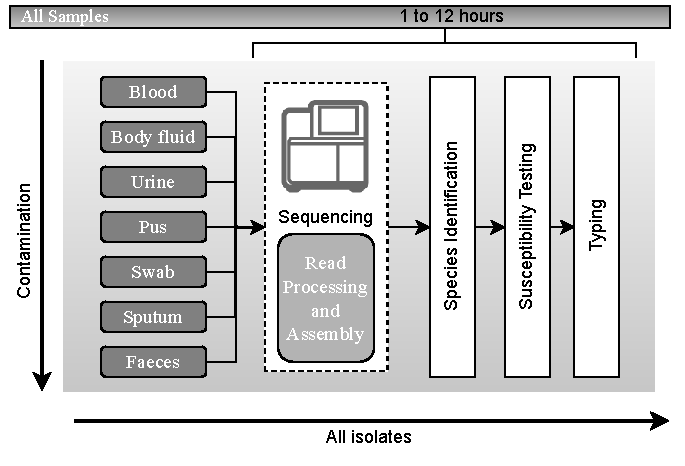
\includegraphics[width=\textwidth]{figures/introduction/Figure 4.pdf}
\caption{\textbf{Hypothetical workflow based on metagenomic sequencing.} Schematic representation of the hypothetical workflow for the direct processing of samples from suspected sources of pathogens after adoption of metagenomic sequencing, with an expected timescale that could fit within a single day. Adapted from \cite{didelot_transforming_2012}}
\label{fig:figure4}
\end{figure*}


Albeit lacking consensus in the field, metagenomics can be classified into two variants as proposed by \citep{marchesi_vocabulary_2015}: (1) metaxonomics where marker genes ubiquitous in many taxa are targeted and sequenced, and (2) the untargeted "shotgun" sequencing of all microbial genomes present in a sample. 

\subsubsection{Metataxonomics and Targeted Metagenomics} \label{sssec:_intro_metataxonomics}

Molecular barcoding approaches can be combined with second-generation high-throughput sequencing to achieve unprecedented depths of coverage in microbial community profiling, being defined as metataxonomics. 
For profiling bacterial species, the most popular approach is 16S \ac{rRNA} gene sequencing, an ~1500 base pair gene coding for a catalytic RNA that is part of the 30S ribosomal subunit. 
Traditionally, the variable regions of the 16S \ac{rRNA} gene (V-regions) are targeted, or ranges thereof (V1-V2, V1-V3, V3-V4, V4, V4-V5, V6-V8, and V7-V9), and are specific to bacterial genus (96\%) and for some, even species (87.5\%), \citep{srinivasan_use_2015, abellan-schneyder_primer_2021}. 
Moreover, dedicated 16S databases that include near full length sequences for a large number of strains and their taxonomic placements exist, such as RDP\footnote{\url{http://rdp.cme.msu.edu/}}, Greengenes\footnote{\url{https://greengenes.secondgenome.com/}}, silva\footnote{\url{https://www.arb-silva.de/}} and NCBI's 16S ribosomal RNA project\footnote{\url{https://www.ncbi.nlm.nih.gov/refseq/targetedloci/}} \citep{cole_ribosomal_2009, desantis_greengenes_2006, pruesse_silva_2007}. 
The sequence from an unknown strain can be compared against the sequences in these databases, after very closely related sequences are grouped into Operational Taxonomic Units (OTUs), and infer likely taxonomy, with the assumption that sequences of $>$95\% identity represent the same genus, whereas sequences of $>$97\% identity represent the same species \citep{schloss_introducing_2005}. 
Additionally, NCBI also provides the 23S ribosomal RNA project for Bacteria and Archaea metataxonomics. 

Additionally, it must necessarily account for intragenomic variation between 16S gene copies. 
Microbial profiles generated using different primer pairs need independent validation of performance, and the comparison of data sets across V-regions using different databases might be misleading due to differences in nomenclature and varying precisions in classification, and specific but important taxa are not picked up by certain primer pairs (e.g., \textit{Bacteroidetes} is missed using primers 515F-944R) or due to the database used \citep{abellan-schneyder_primer_2021}. 
Furthermore, targeting of 16S variable regions with short-read sequencing platforms cannot achieve the taxonomic resolution afforded by sequencing the entire (~1500 \ac{bp}) gene \citep{johnson_evaluation_2019}. 
The emergence of third generating sequencing technologies (see \secref{ssec:_intro_3rd_gen_seq}) allows for this limitation to be overcome but currently, only a fraction of the databases includes complete 16S \ac{rRNA} sequences.

While viruses are an integral part of the microbiota, no universal viral marker genes are available to perform such taxonomic assignments. 
Amplification of whole viral genomes is possible and, in 2015, RNA extracted from whole blood, serum, re-suspended swabs and urine, after targeted amplification of the whole viral genome, proved invaluable in the track of the Ebola virus disease epidemic in West Africa, responsible for >11 thousand deaths, allowing for the characterisation of the infectious agent the determination of its evolutionary rate, signatures of host adaptation, identification and monitoring of diagnostic targets and responses to vaccines and treatments \citep{quick_real-time_2016}.
As an alternative, broad scope viral targeted sequence capture (TSC) panels offer depletion of background nucleic acids and improve the recovery of viral reads by targeting coding sequence from a multitude viral genera, such as VirCapSeq-VERT Capture Panel\footnote{\url{https://sequencing.roche.com/content/dam/rochesequence/worldwide/resources/brochure-vircapseq-vert-capture-panel-SEQ1000117.pdf}} but do not guarantee the full recovery of the viral genome, and can present biases towards certain genera \citep{schuele_assessment_2020, wylie_enhanced_2015}. 

\subsubsection{Shotgun Metagenomics} \label{sssec:_intro_shotgun_metagenomics}

Shotgun metagenomics can offer relatively unbiased pathogen detection and characterisation. The capacity to detect all potential pathogens — bacteria, viruses, fungi and parasites — in a sample has great potential utility in the diagnosis of infectious disease \citep{chiu_clinical_2019}, potentially able to provide genotyping, antimicrobial resistance and virulence profiling in a single methodological step. This comes with the cost of producing massive amounts of information that require expert handling and processing, as well as capable computational infrastructures \citep{couto_critical_2018, rossen_practical_2018}.

Clinical applications of shotgun metagenomics derive its roots from the use of microarrays (see \secref{ssec:_intro_current_standards}), where it was successfully applied in in-depth microbiome analysis of different sites in the human body, it was the emergence of second-generation sequencing technology and its high throughput of genomic data at a competitive price that made the sequencing of all genomic content, DNA and/or RNA) if a clinical sample a viable possibility for diagnostics (see \secref{ssec:_intro_2nd_gen_seq}) \citep{miller_basic_2009, palmer_rapid_2006, chiu_clinical_2019}. The first reported case that demonstrated the utility of shotgun metagenomics was in 2014 with the clinical diagnosis of neuroleptospirosis in a 14-year-old immunodeficient and critically ill boy with meningoencephalitis by \cite{wilson_actionable_2014}, prompting appropriate targeted antibiotic treatment and eventual recovery of the patient. In this case, traditional methods, including an invasive brain biopsy, failed to provide answers, until the shotgun sequencing of cerebrospinal fluid identified 475 of 3,063,784 sequence reads (0.016\%) corresponding to leptospira, for which clinical assays were negative due to its very low abundance. Ever since many other reports of successful application of shotgun metagenomics in clinical metagenomics have been reported. but all in edge cases where traditional diagnostic methods have failed or as proof-of-concept \citep{couto_critical_2018, vijayvargiya_application_2019, sanabria_shotgun-metagenomics_2020, hirakata_application_2021}. 

In public health microbiology, shotgun metagenomics combined with transmission network analysis allowed the investigation and quick action on the food supply of the 2013 outbreak of Shiga toxin-producing \textit{Escherichia coli} (STEC) strain O104:H4 from faecal specimens obtained from patients \citep{loman_culture-independent_2013}. A similar approach was followed in the detection of \textit{Salmonella enterica} subsp. \textit{enterica} serovar Heidelberg from faecal samples in two though to be unrelated outbreaks in the United States of America, as well as the \textit{in situ} abundance and level of intrapopulation diversity of the pathogen, and the possibility of co-infections with \textit{Staphylococcus aureus}, overgrowth of commensal \textit{Escherichia coli}, and significant shifts in the gut microbiome during infection relative to reference healthy samples \citep{huang_metagenomics_2017}. More recently, shotgun metagenomic sequencing has evidenced alterations in the gut microbiota of a subset of COVID-19 patients that present the uncommon gastrointestinal (GI) symptoms, shedding a higher understanding of gut–lung axis affecting the progression of COVID-19 \citep{li_microbiome_2021}.

Clinical diagnostic applications have lagged behind research advances. A significant challenge with shotgun metagenomic approach is the large variation in the pathogen load between patient samples, as evidenced in the studies presented. A low pathogen load and  high contamination of host DNA or even the present microbiome may result in enough data to produce the high-resolution subtype needed to distinguish and cluster the cases that were caused by the same outbreak pathogen source, or, extremely, the undetection of the causative agent \citep{carleton_metagenomic_2019, chiu_clinical_2019}. Differential lysis of human host cells followed by degradation of background DNA has proven an effective method to reduce host contamination, but limitations include potential decreased sensitivity for microorganisms without cell walls, such as \textit{Mycoplasma} spp. or parasites; a possible paradoxical increase in exogenous background contamination by use of additional reagent \citep{salter_reagent_2014, oneil_ribosomal_2013, feehery_method_2013}. Additionally, it is often unclear whether a detected microorganism is a contaminant, coloniser or \textit{bona fide} pathogen, and the lack of golden standards remains one of the biggest challenges when applying these methods in clinical microbiology for diagnosis. 

In addition to negative controls, already a common practice in any sequencing assay and in particular in metataxonomics (see \secref{sssec:_intro_metataxonomics}), positive controls can be a way to circumvent the lack of golden standards, either through the spike of the samples with a known amount of a specific DNA/RNA or though the sequencing of samples with known composition and abundance. Well-characterised reference standards and controls are needed to ensure shotgun metagenomics assay quality and stability over time \citep{chiu_clinical_2019, mcintyre_comprehensive_2017}. Most available metagenomic reference materials are highly tailored to a specific application. For example, the ZymoBIOMICS Microbial Community Standard\footnote{\url{https://www.zymoresearch.com/collections/zymobiomics-microbial-community-standards}} is the first commercially available standard for microbiomics and metagenomics studies, providing mock a mock community with defined composition and abundance consisting of Gram-positive, Gram-negative and yeast. It is useful to determine the limit of detection of an assay, and the effectiveness and biases of a given protocol. Standards with a more limited spectrum of organisms are also available, such as the National Institute of Standards and Technology (NIST)\footnote{\url{https://www.nist.gov/}} reference materials for mixed microbial DNA detection, which contain only bacteria. Thus, these materials may not apply to untargeted shotgun metagenomics analyses.

\section{The role of bioinformatics} \label{sec:_intro_bioinformatics}

As stated previously (see \secref{sec:_intro_genomics_approach} and \secref{ssec:_intro_metagenomics}), one of the biggest challenges when dealing with genomic, and in particular metagenomic, data is the lack of golden standards. This is also applicable to the bioinformatic analysis, required due to the amount of data produced by genomic sequencing technologies. This is currently one of the bottlenecks in the deployment of sequencing technology in clinical microbiology as there's no standard in how to deal with the increasing amount of data produced in a fit-for-purpose manner \citep{carrico_primer_2018}.

Bioinformatics is an interdisciplinary research field that applies methodologies from computer science, applied mathematics and statistics to the study of biological phenomena\citep{carrico_primer_2018}. With the widespread use and continuous development of sequencing technologies, bioinformatics has become a cornerstone in modern clinical microbiology. 

Major efforts are being made on the standardisation and assessment of software for the analysis of genomic data, both commercial and open-source \cite{angers-loustau_challenges_2018, gruening_recommendations_2019, sczyrba_critical_2017, couto_critical_2018}. 

\subsection{The FASTQ file} \label{ssec:_intro_fastq}

In all sequencing technologies (see \secref{ssec:_intro_sequencing}), many copies of the source DNA are randomly fragmented and sequenced. To these sequences, we refer to as reads. In the case of second-generation sequencing (see \secref{ssec:_intro_2nd_gen_seq}), one or both ends of the fragment can be sequenced. If a fragment is sequenced from one end, we refer to it as single-end sequencing. If a fragment is sequenced on both ends, spanning the entire fragment, it is called paired-end sequencing.

All sequencing technologies, regardless of generation, produce data in the same standard file format: the FASTQ, a text-based format for storing both a biological sequence (usually nucleotide sequence) and its corresponding quality scores \citep{cock_sanger_2010}. Originally developed at the Wellcome Trust Sanger Institute, the FASTQ has emerged as a common file format for sharing sequencing read data (see \ref{fig:figure3}). The FASTQ can be considered as an extension of the ‘FASTA sequence file format’, originally invented by \cite{pearson_improved_1988}, which includes just the sequence information. A FASTQ file normally uses four lines per sequence:

\begin{itemize}
    \item \textbf{Line 1} begins with a '@' character and is followed by a sequence identifier and an optional description;
    \item \textbf{Line 2} is the raw sequence letters;
    \item \textbf{Line 3} begins with a '+' character and is optionally followed by the same sequence identifier (and any description) again;
    \item \textbf{Line 4} encodes the quality values for the sequence in Line 2, and must contain the same number of symbols as letters in the sequence.
\end{itemize}

In FASTQ both the sequence letter and quality score are each encoded with a single ASCII character for brevity. The quality of a sequence in a FASTQ file is represented by a quality value Q is an integer mapping of p, where p is the probability that the corresponding base call is incorrect (see Table \ref{tab:phred_error}). This is called the PHRED score \citep{ewing_base-calling_1998} and is defined by the following equation:

\begin{equation}
\centering
\mathbf{Q}\textsc{phred} = - 10 \times \log \mathbf{P}
\end{equation}
 
The PHRED quality scores $\mathbf{Q}$ is defined as a property which is logarithmically related to the base-calling error probability $\mathbf{P}$.

\begin{table}[h!]
\caption{\textbf{PHRED quality scores are logarithmically linked to error probabilities.} A PHRED Score of 20 indicates the likelihood of finding 1 incorrect base call among 100 bases. In other words, the precision of the base call is 99\%. $\mathbf{Q}$ scores are classified as a property that is associated logarithmically with the probabilities of base calling error $\mathbf{P}$.} \label{tab:phred_error}
\begin{tabular}{@{}lll@{}}
\toprule
\textbf{Phred Quality Score} & \textbf{Probability of incorrect base call} & \textbf{Base call accuracy} \\ \midrule
10 & 1 in 10        & 90\%     \\
20 & 1 in 100       & 99\%     \\
30 & 1 in 1000      & 99.90\%  \\
40 & 1 in 10,000    & 99.99\%  \\
50 & 1 in 100,000   & 100.00\% \\
60 & 1 in 1,000,000 & 100.00\% \\ \bottomrule
\end{tabular}
\end{table}

Since their introduction, PHRED scores have become the \textit{de facto} standard for representing sequencing read base qualities \citep{cock_sanger_2010}. Despite this convention, the encoding of the Phread score can vary when it is translated to its ASCII representation in the FASTQ file format. For example, the Sanger FASTQ files use ASCII 33–126 to encode PHRED qualities from 0 to 93 (i.e. PHRED scores with an ASCII offset of 33). A full list of available encoding is available in \ref{fig:figure6}. 

\begin{figure*}[h!]
\centering
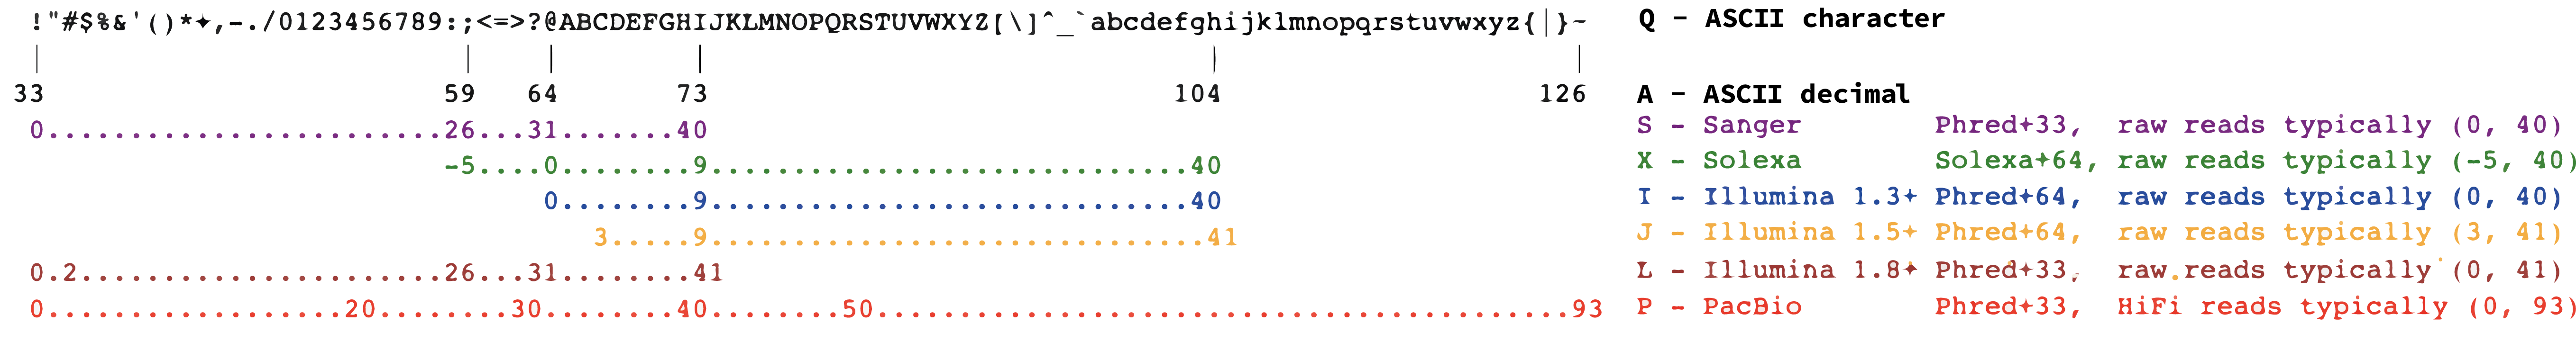
\includegraphics[width=\textwidth]{figures/introduction/Figure 6.png}
\caption{\textbf{Range of FASTQ quality scores andd their corresponding ASCII encoding.} For raw reads, the range of scores will depend on the technology and the base caller used. Starting in Illumina 1.8, the quality scores have returned to the use of the Sanger format (PHRED+33). For processed reads and long accurate reads, scores may be even higher with, For example, quality values of up to 93 observed in reads from PacBio HiFi reads.}
\label{fig:figure6}
\end{figure*}

\subsubsection{FASTQ file simulation} \label{ssec:_intro_fastq_sim}

With the lack of golden standards for metagenomic analysis, the use of simulated mock communities, with known composition, abundance and genomic information, provides a ground truth against which evaluations of success can be made. Given their standard structure and adoption, the generation of simulated FASTQ files from a reference, or a set of references, is very straightforward. 

Multiple computational tools for the simulation of sequencing data, particularly for second and third-generation sequencing technologies, have been developed in recent years, which could be used to compare existing and new bioinformatic analytical pipelines. \cite{escalona_comparison_2016} provides a comprehensive assessment of 23 different read-simulation tools,  highlighting their distinct functionality, requirements and potential applications, as well as providing a selection of suggestions for different simulation tools depending on their purpose. For \textit{in silico} genomic and metagenomic sequence generation, a pletora of tools are available for first, second and third-generation reads (see Figure \ref{fig:figure7}).

\begin{figure*}[h!]
\centering
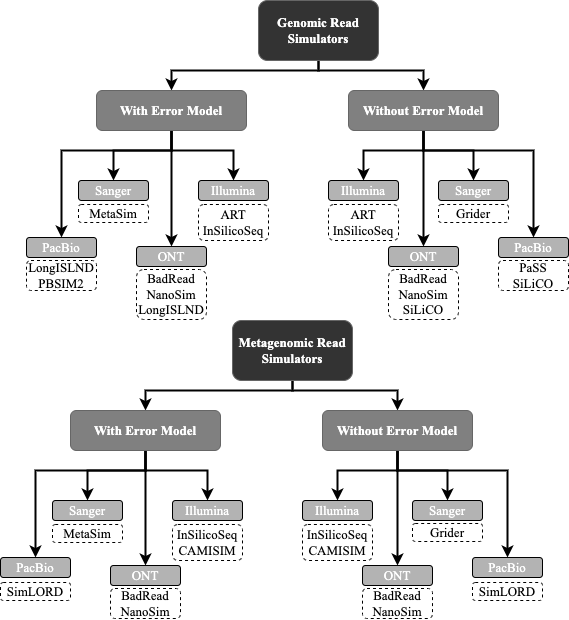
\includegraphics[width=\textwidth]{figures/introduction/Figure 7.png}
\caption{\textbf{Sequence simulators for genomic and metagenomic data.} For first generation sequencing, Metasim (\url{https://github.com/gwcbi/metagenomics_simulation}) and Grider (\url{https://sourceforge.net/projects/biogrinder/}) can generate mock genomic and metagenomic data, with and without error models respectively. For Illumina data, ART (\url{https://www.niehs.nih.gov/research/resources/software/biostatistics/art/index.cfm}), InSilicoSeq (\url{https://github.com/HadrienG/InSilicoSeq}) and CAMISIM (\url{https://github.com/CAMI-challenge/CAMISIM}) represent options for in silico data generation. Due to their differences, the third generation Pacific BioSciences (PacBio) and Oxford Nanopore (ONT) have distict software for in silico data generation. The first can be accomplished by LongISLND (\url{https://bioinform.github.io/longislnd/}) and PBSIM2 (\url{https://github.com/yukiteruono/pbsim2}) got genomic data, and SimLORD (\url{https://bitbucket.org/genomeinformatics/simlord/src}) fot metagenomic data, with and without error model. The latter BadRead (\url{https://github.com/rrwick/Badread}) and NanoSim (\url{https://github.com/bcgsc/NanoSim}) can genenrate genomic and metagenomic \textit{in silico} data, with and withouth error model. Additionally, for genomic data, LongISLND and SiLiCO (\url{https://github.com/ethanagb/SiLiCO}) generate data with and without error, respectively. Adapted from \cite{escalona_comparison_2016}.}
\label{fig:figure7}
\end{figure*}

\subsubsection{FASTQ quality assessment and quality control} \label{ssec:_intro_fastq_quality}

Quality assessment and control is a basal step to any analysis, and aims to (1) remove and/or filter low quality and low complexity reads, (2) trim adapters, and (3) remove host sequences from the samples’ raw data. There are many tools available but the most commonly used are FastQC\footnote{\url{https://www.bioinformatics.babraham.ac.uk/projects/fastqc/}} (Babraham Bioinformatics) for quality control, followed by Trimmomatic \citep{bolger_trimmomatic_2014}, Cutadapt \citep{martin_cutadapt_2011} or fastp \citep{chen_fastp_2018} to trim and/or filter adaptors, low quality and low complexity sequences. For long-read sequencing, tools like NanoPlot and NanoStats \citep{de_coster_nanopack_2018}, and Filtlong\footnote{\url{https://github.com/rrwick/Filtlong/}} can perform the equivalent quality assessment and control, adapter trimming and low quality trimming, respectively. 

\subsection{Direct taxonomic assignment and characterisation} \label{ssec:_intro_taxonomic_assignment}

A piece of important information that can be retrieved directly from the quality-controlled read data: (1) the identification and characterisation of the microbes present in a sample and (2) their relative abundance. Taxonomic classification methods can vary depending on the sequencing methodology used: pure culture, metataxonomics and amplicon metagenomics, and shotgun metagenomics.

From pure culture, taxonomic identification of the read content of a sample is useful to assess contamination. Tools like Kraken2 \citep{wood_kraken_2014, wood_improved_2019} and Braken \citep{lu_bracken_2017}. These tools, relying on a database, assign taxonomic labels to reads and are therefore biased to the contents of the database used. Various databases are available\footnote{\url{https://benlangmead.github.io/aws-indexes/k2}}, varying in size and content (archaea, bacteria, viral, plasmid, human and eukaryotic pathogens), and therefore in sensitivity depending on the resources available and the purpose intended. Alternatively, there are options to create custom databases.  

These tools are also extremely useful to assess the contents of a metagenomic sample. Alternatives such as Midas \citep{nayfach_integrated_2016}, Kaiju, \citep{menzel_fast_2016}, and MetaPhlAn2 \citep{truong_metaphlan2_2015} offer the same analysis as Kraken and Bracken using different algorithms, and with the disadvantage that they come prepackaged with their own databases, without the option to create a tailored database, limiting their applicability. Kaiju differs from the other tools by using a protein reference database, instead of nucleotide, but no pre-built version is available, requiring significant resources to build and index the database pre-use. The long-read data of third-generation sequencing technologies (see \secref{ssec:_intro_3rd_gen_seq}) can be treated as single-end reads, and all tools mentioned accommodate the classification of single-end files. 

\subsection{From reads to genomes} \label{ssec:_intro_reads_2_genomes}

Due to the limitations of current sequencing technologies (see \secref{ssec:_intro_sequencing}), the order of the reads produced by these machines cannot be preserved. 
Therefore, to obtain the true original genomic sequence the process of "genome assembly" has to occur. 
The term "draft genome" is commonly used because these sequencing technologies do not generate a single closed genome, particularly short-read such as in second generation sequencing (see \secref{ssec:_intro_2nd_gen_seq}) which need to be assembled into usually a series of sequences (contigs) that may cover up to 95\% to 99\% of the strain genome \citep{carrico_primer_2018}. 
Long-read technologies (see \secref{ssec:_intro_3rd_gen_seq}) allow for this value to reach 100\%, effectively producing closed, complete genomes, notwithstanding that this value can sometimes overcome the 100\% due to overlap \citep{wick_benchmarking_2021}. 

Assembling reads into contigs has many advantages, namely that longer sequences are more informative, allowing the consideration of whole genes or even gene clusters within a genome and to understand larger genetic variants and repeats. Additionally, it has the effect of removing most sequencing errors, though this can be at the expense of new assembly errors \citep{ayling_new_2020}. Two methods are used to obtain draft genomes: (1) through reference-guided sequence assembly, or (2), through \textit{de novo} sequence assembly.

\subsubsection{Genomes through reference-guided sequence assembly}

A reference-guided genome assembly uses an already sequenced reference genome to assemble a new genome, making use of the similarity between target and reference species to gain additional information, which often lead to a more complete and improved genome \citep{rausch_consistency-based_2009, lischer_reference-guided_2017}. 
This process is usually done through the mapping of the reads to a closely related reference sequence, and as more and more species get sequenced, the chance that a genome of the same or related species is already available, in which a significant proportion of the reads can be mapped, increase greatly. 
This process usually includes the following steps: (1) the reference genome has to be indexed, allowing compression of the input text while still permitting fast sub-string queries, (2) for each short-read several sub sequences (seeds) are taken and searched to find their exact matches in the reference  (candidate regions), (3) each short-read is then aligned to all corresponding candidate regions, and (4) the consensus sequence is computed in which the reference sequence is corrected when there is enough evidence of an difference based on the mapped
reads, identifying the differences between it and the newly generated consensus sequence \citep{bayat_methods_2020}.
Besides variants, the new consensus genome might have insertions or deletions with respect to the reference genome.

Besides the generation of a consensus sequence, the mapping of the reads to the reference sequence can be used to estimate sequence depth and breadth of coverage. 
Depth of coverage, often referred to simply as coverage, refers to the average number of times each nucleotide position in the strain's genome has a read that aligns to that position. Depending on the study goals, bacterial species and the intended analyses, the optimal depth of coverage varies. 
In public repositories, most submissions have a depth of coverage ranging from 15 to 500 times \citep{carrico_primer_2018}. 
Breadth of coverage is defined as the ratio of covered sequence on the reference by the aligned reads.

\subsubsection{Genomes through \textit{de novo} sequence assembly}

De novo assembly refers to the bioinformatics process whereby reads are assembled into a draft genome using only the sequence information of the reads. Two methods are used to obtain draft genomes without the need of a reference genome: (1) through Overlap, Layout and Consensus, or (2) De Bruijn graph assembly (see Figure \ref{fig:figure8}). The \textit{de novo} assembly methods provide longer sequences that are more informative than shorter sequencing data and can provide a more complete picture of the microbial community in a given sample.

\begin{figure*}[h!]
\centering
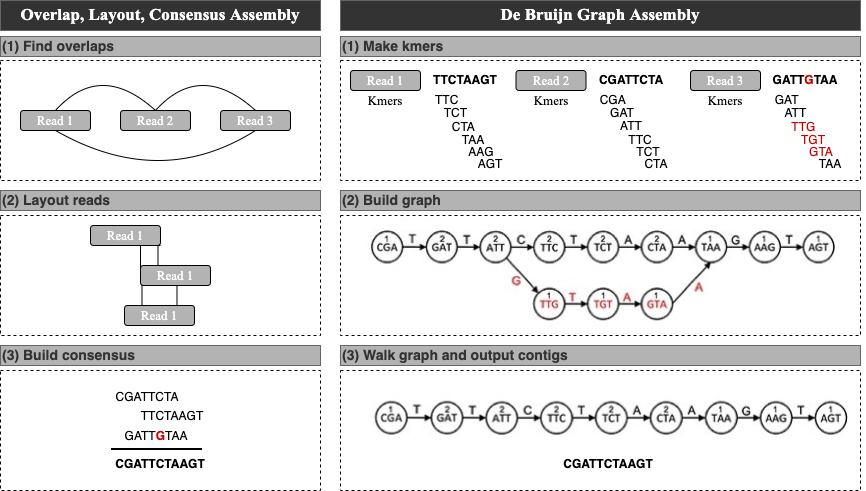
\includegraphics[width=\textwidth]{figures/introduction/Figure 8.png}
\caption{\textbf{Approaches to \textit{de novo} genome assemble.} In Overlap, Layout, Consensus assembly, (1) overlaps are found between reads and an overlap graph constructed (edges indicate overlapping reads). (2) Reads are laid out into contigs based on the overlaps (lines indicate overlapping portions). (3) The most likely sequence is chosen to construct consensus sequence. In De Bruijn graph assembly, (1) reads are decomposed into kmers of a determined size by sliding a window of size k (in here of k=3) across the reads. (2) The kmers become vertices in the De Bruijn graph, with edges connecting overlapping kmers. Polymorphisms (red) form branches in the graph. A count is kept of how many times a kmer is seen, shown here as numbers above kmers. (3) Contigs are built by walking the graph from edge nodes. A variety of heuristics handle branches in the graphs—for example, low coverage paths, as shown here, may be ignored. Adapted from \cite{ayling_new_2020}}.
\label{fig:figure8}
\end{figure*}

\paragraph{Overlap, Layout and Consensus assembly} \label{sssec:_intro_OLC_assembly} \mbox\\

First generation sequencing technology (see \secref{ssec:_intro_1st_gen_seq}) produces far fewer reads than second generation sequencing technology (see \secref{ssec:_intro_2nd_gen_seq}, but individual reads are longer (500–1000 \ac{bp}). 
Assembly of Sanger data usually uses overlap-layout consensus (OLC) approaches, in which:

\begin{itemize}
    \item Overlaps are computed by comparing all reads to all other reads;
    \item Overlaps are grouped together to form contigs;
    \item A consensus contiguous sequence, or contig, is determined by picking the most likely nucleotides from the overlapping reads.
\end{itemize}

These type of assemblers were very popular in the early 2010s, with assemblers such as Celera\footnote{\url{https://www.cbcb.umd.edu/software/celera-assembler}},  Genovo\footnote{\url{https://cs.stanford.edu/genovo }}, xGenovo\footnote{\url{http://xgenovo.dna.bio.keio.ac.jp/}} and BBAP\footnote{\url{http://homepage.ntu.edu.tw/~youylin/BBAP.html}} having been widely used \citep{myers_whole-genome_2000, hutchison_genovo_2010, afiahayati_extended_2013, lin_novo_2017}.
With the emergence of third-generation sequencing (see \secref{ssec:_intro_3rd_gen_seq}), OLC assemblers have been increasingly developed and adopted by the community to assembly long-read data. 
In the latest years, ra\footnote{\url{https://github.com/lbcb-sci/ra}}, raven\footnote{\url{https://github.com/lbcb-sci/raven}} and canu\footnote{\url{https://github.com/marbl/canu}}, the latter being a a fork of the Celera Assembler, have become staples in the community, showing good reliability and amassing over 3000 citations \citep{vaser_yet_2019, koren_canu_2017, wick_benchmarking_2021}.  %missing raven

\paragraph{De Bruijn graph assembly} \label{sssec:_intro_dbg_assembly} \mbox{}\\

In the De Bruijn assembly graph, reads are split into overlapping k-mers where nodes of the graph represent k-mers where:

\begin{itemize}
    \item A directed edge from node N\textsubscript{a} to node N\textsubscript{b} indicates that N\textsubscript{b} is next to N\textsubscript{a} in a read;
    \item The number of nodes in the De Bruijn graph is theoretically the total number of identical k-mers in the genome;
    \item The weight on the edge indicates the number of times  N\textsubscript{b} is observed next to  N\textsubscript{a} in all reads.
\end{itemize}

Thus, the weight of an edge indicates the possibility that two k-mers appear after each other in the DNA sequence. A path in the graph where all edges have the highest weight is the most likely to be a part of the genome \citep{bayat_methods_2020}.

Most second-generation sequencing (see \secref{ssec:_intro_2nd_gen_seq} assemblers, such as SPAdes\footnote{\url{https://github.com/ablab/spades/}}, SKESA\footnote{\url{https://github.com/ncbi/SKESA/}} and MEGAHIT\footnote{\url{https://github.com/voutcn/megahit/}}, use a multiple k-mer De Bruijn graph, starting with the lowest size and iteratively adding k-mers of increasing length to connect the graph \citep{bankevich_spades_2012, souvorov_skesa_2018, li_megahit_2015}. Older assemblers, such as Velvet\footnote{\url{https://www.ebi.ac.uk/~zerbino/velvet/}}, Ray\footnote{\url{https://sourceforge.net/projects/denovoassembler/f}} and SoapDeNovo2\footnote{\url{https://sourceforge.net/projects/soapdenovo2/}} use a single k-mer strategy for the De Bruijn graph construction \citep{zerbino_velvet_2008, boisvert_ray_2010, luo_soapdenovo2_2012}. 

\subsubsection{Assembly quality assessment and quality control} \label{ssec:_intro_assembly_quality}

The success of an assembly is evaluated in two steps: (1) globally, through intrinsic characteristics of the assembly itself, and (2) relative to a reference genome. The computation of the global metrics is performed through statistics inherent to the complete set of contigs assembled per sample, independent of the species/sample of origin. Commonly, these statistics include information on contig number, its median size and number ambiguous bases. The comparison with a reference sequence allows for statistics such as number of misassemblies, meaning contigs that do not reflect the structural organisation in the reference sequence, to be computed. 

The assessment and evaluation of genome assemblies has been a relevant field ever since the emergence of the assembly process itself. 
The most widely adopted is QUAST\footnote{\url{http://quast.sourceforge.net/quast}}, can evaluate assemblies both with a reference genome, as well as without a reference, producing many reports, summary tables and plots to help compare and assess assembly success \citep{gurevich_quast_2013}. 

\subsection{Reproducibility and transparency} \label{ssec:_intro_reproducibility}

Several steps that can be implemented to ensure the transparency and reproducibility of the chosen bioinformatic workflow. 
Favouring open-source tools, with clear documentation describing the methodology implemented, and stating the version of the software used and which parameters were used enables the comparison of results. 
This can be simplified by containerising all the software tools with one of the many solutions available, like Docker\footnote{\url{https://www.docker.com/}} or Singularity\footnote{\url{https://sylabs.io/}} \citep{kurtzer_singularity_2017}. 

The use of workflow managers, like nextflow\footnote{\url{https://www.nextflow.io/}}, snakemake\footnote{\url{https://snakemake.github.io/}} or the Galaxy Project\footnote{\url{https://galaxyproject.org/}}, will push reproducibility to the next level by taking advantage of the containerisation and scalability, enabling the workflow to be executed with the same parameters in the same conditions in a multitude of different environments \citep{di_tommaso_nextflow_2017, molder_sustainable_2021, afgan_galaxy_2018}. 


\section{Bioinformatic Analysis for Metagenomics} \label{sec:_intro_metagenomics_bioinfo}

As mentioned previously (see \secref{ssec:_intro_metagenomics}, Metagenomic shotgun sequencing circumvents the need for cultivation and, compared with metataxonomics, avoids biases from primer choice, enables the detection of organisms across all domains of life and \textit{de novo} assembly of genomes and functional genome analyses. However, highly uneven sequencing depth of different organisms and low depth of coverage per species are drawbacks that limit taxa

\subsubsection{Metataxonomics} \label{ssec:_intro_metataxonomics_bioinfo}

Metataxonomics (see \secref{sssec:_intro_metataxonomics}) is the most widely used technique for microbial diversity analysis \citep{hilton_metataxonomic_2016}, and due to its particularities, the analysis of this data is also very particular. Data analyses are mostly carried out through specialised pipelines that wrap and combine several tools, offering the possibility to follow a simple protocol with default configurations or choose between a plethora of different configurations to adjust for any particular needs. Quantitative Insights Into Microbial Ecology 2 (QUIIME2)\footnote{\url{https://qiime2.org/}} \citep{bolyen_reproducible_2019} has become the \textit{de facto} tool for metataxonomic analysis as a framework with an ever-growing suite of plugins and intuitive data visualisation tools for the assessment of results. Mothur \citep{schloss_introducing_2009} and UPARSE \citep{edgar_uparse_2013} are also a popular alternative although resulting outputs differing significantly between pipelines despite using the same inputs having been reported by \cite{marizzoni_comparison_2020}, with a magnitude that is comparable to differences in upstream sample treatment and sequencing procedures.  A typical workflow starts with quality filtering, error correction and removal of chimeric sequences. These quality control steps are followed by either taxonomic assignment of reads or a clustering step where reads are gathered into OTUs given their sequence identity, followed by statistical analysis to assess differences between given groups. Taxonomic assignment methods classify query sequences based on the best hit found in reference databases of annotated sequences, being heavily dependent on the completeness of the reference databases (see \secref{sssec:_intro_metataxonomics}). Classification is further limited by lack of species annotation in most reference databases \citep{westcott_novo_2015}. Alternatively, the same approach of direct taxonomic classification, without OTU clustering, can be followed as with genomic and shotgun metagenomic data, given that the databases include \ac{rRNA} sequences.

OTU clustering methods can be categorised into: (1) computationally expensive hierarchical methods that cluster sequences based on a distance matrix measuring the difference between each pair of sequences, (2) less expensive heuristic methods cluster sequences into OTUs based on a pre-defined threshold, generally, with a sequence being selected as a seed and the rest of the sequences being analysed sequentially and added to existing or new clusters according to the defined threshold, and (3) model based clustering methods that do not rely on a pre-defined and fixed threshold, defining OTUs based on a soft threshold and carrying out the clustering process based on methods such as an unsupervised probabilistic Bayesian clustering algorithm \citep{hao_clustering_2011}. These methods offer the possibility to cluster sequences based on criteria that do not depend on reference databases and are especially useful in less characterised microbial communities or with a high representation of uncultured microbes. Due to the assumptions made with this strategy, it is sensitive to under or overestimation of the number of OTUs in a sample as defining a threshold to accurately cluster sequences is difficult \citep{westcott_novo_2015}.

\subsubsection{Shotgun metagenomics} \label{ssec:_intro_shotgun_metagenomics_bioinfo}

A plethora of open-source tools are available specifically for shotgun metagenomic data, and several combinations of these tools can be used to characterise the causative agent in a patient's infection in a fraction of the time required by the traditional methods. 

A major additional difficulty of shotgun metagenomic data is the overpowering quantities of host DNA that are often sequenced, making the microbial community sometimes close to undetectable \citep{couto_critical_2018}.
The presence of contaminants, from the bench process to the pre-existing biota, and the cost associated with this methodology, are also major hinders in its applicability in the clinic.
They account for major caveats and must be made aware of when analysing the data.

\begin{figure*}[h!]
\centering
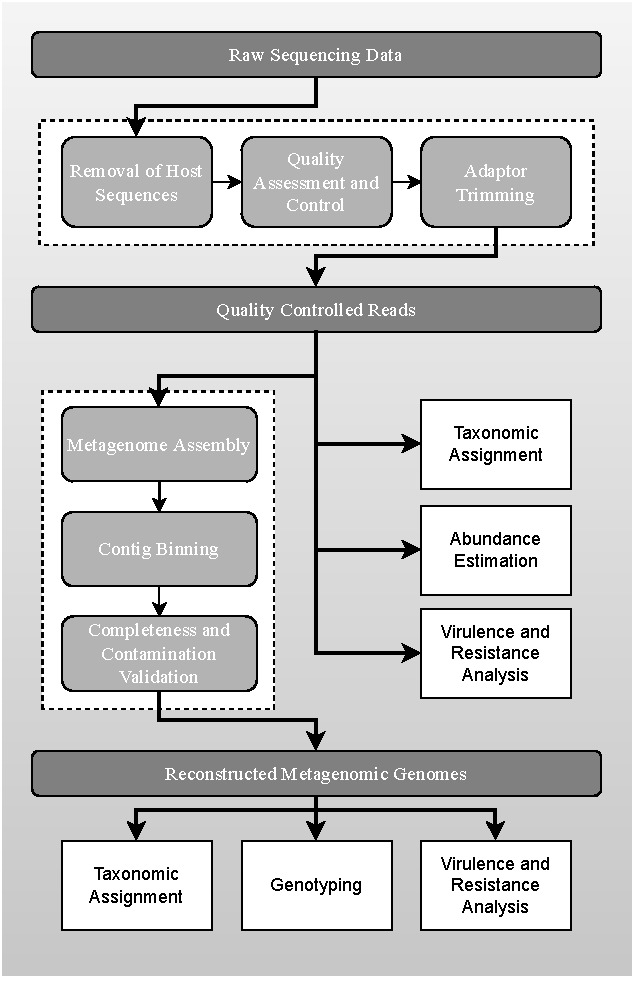
\includegraphics[]{figures/introduction/Figure9.pdf}
\caption{Typical bioinformatic analysis procedure for metagenomic data}
\label{fig:figure9}
\end{figure*}

The basic strategies for analysing shotgun metagenomic data can be simplified in the scheme in Figure \ref{fig:figure9}. 
One of the biggest challenges when doing metagenomic analysis is differentiating between colonisation and infection by successfully discriminating between a potential pathogen and background microbiota. 
In the latter, when analysing samples from presumably sterile sites, like Cerebrospinal fluid (CSF) and blood, it is safe to assume that all organisms found are of interest. 
In locations with a microbiota, the inclusion of negative controls is essential for the correct identification of contaminants in the taxonomic results, whether originated from the sample collection, handling or sequencing process. 
The use of spiked metagenomic samples as positive control might guide the detection of the possible pathogens by comparing relative abundance between the samples. 
These controls should be processed similarly to the samples and the taxonomic results should be filtered out from the final report. 

As explored in \secref{ssec:_intro_reads_2_genomes}, longer sequences are more informative than shorter sequencing data, as the one obtained from second-generation sequencing (see \secref{ssec:_intro_2nd_gen_seq}), and can provide a more complete picture of the microbial community in a given samples. 
Several dedicated metagenomic assembly tools are available, such as metaSPAdes\footnote{\url{https://github.com/ablab/spades/}}  and MegaHIT\footnote{\url{https://github.com/voutcn/megahit/}} \citep{nurk_metaspades_2017, li_megahit_2015}. 
These tools, in comparison to single-cell data assemblers, are better at dealing with the combination of intra and intergenomic repeats and uneven sequencing coverage \citep{olson_metagenomic_2017}.
For third-generation sequencing, dedicated metagenomic assemblers have recently emerged, such as meta-flye\footnote{\url{https://github.com/fenderglass/Flye/}} which expands on the original flye assembler by overcoming a k-mer selection limitation on low abundance species \citep{kolmogorov_metaflye_2020}. Nevertheless, the use of non dedicated assemblers for metagenomics may come with the cost of wrongly interpret variation as error, especially in samples that contained closely related species and the construction of chimeric sequences as traditional assemblers follow the basic principle that the coverage in a sample is constant \citep{teeling_current_2012}. 

The assembly-based approach requires the grouping of the different contigs into bins, ideally each collecting the sequences that belong to a microorganism present in the sample. The binning process can be taxonomy dependent, relying on a database to aggregate the sequences, or independent. The independent approach has the benefit of not relying on a database, but instead it uses the composition of each sequence and coverage profiles to cluster together sequences that might belong to the same organism. These algorithms don’t require prior knowledge about the genomes in a given sample, instead relying on features inherent to the sequences in the sample. Although most binning software can work with single metagenomic samples, most make use of differential coverage of multiple samples to improve the binning process \citep{sedlar_bioinformatics_2017}. It allows the handling of complex ecosystems and might be crucial when analysing samples recovered from sites with a complex microbiota. A comparison of five taxonomic independent  and four taxonomic binning software by \cite{sczyrba_critical_2017} revealed that, for taxonomic independent approaches, MaxBin2\footnote{\url{https://sourceforge.net/projects/maxbin2/}} had the highest completeness and purity in the bins obtained \citep{}. For taxonomic binning, working similarly to the direct taxonomic assignment of the sequencing data, PhyloPythiaS+\footnote{\url{https://github.com/algbioi/ppsp}} obtained better results in accuracy, completeness and purity, followed by Kraken\footnote{\url{https://github.com/DerrickWood/kraken2/}} that still obtained decent results with the added benefit of very high speed of analysis, ease of use and inclusion of the pre-built databases \citep{gregor_phylopythias_2016, wood_kraken_2014}.

 

\newpage
\section{References}
\printbibliography[heading=none]
\end{refsection}


%-----------------------------------------------------------------
% Paper 1 - Natacha
%------------------------------------------------------------------
\newpage
\thispagestyle{empty}
\chapter{Critical steps in clinical shotgun metagenomics for the concomitant detection and typing of microbial pathogens\label{ch:paper1}}

\thispagestyle{empty}
\clearpage \thispagestyle{empty}\mbox{}\clearpage
\newpage
\begin{refsection}
\mbox{}\\
\vspace{8cm}

This chapter is a reproduction of the following publication:

N. Couto, L. Schuele, E.C. Raangs, M. P. Machado, C. I. Mendes, T. F. Jesus, M. Chlebowicz,  S. Rosema, M. Ramirez, J. A. Carriço, I. B. Autenrieth, A. W. Friedrich, S. Peter and J. W. Rossen. Critical steps in clinical shotgun metagenomics for the concomitant detection and typing of microbial pathogens. Sci Rep 8, 13767 (2018). \url{https://doi.org/10.1038/s41598-018-31873-w}

The supplementary information referred throughout the text can be consulted in
this chapter before the section of references. 

As mentioned in Chapter \ref{sssec:shotgun_metagenomics}, shotgun metagenomic (SMg) approaches have been a growing interest to deliver clinically relevant results without \textit{a priori} knowledge of what to expect from a particular clinical sample or patient. 
The capacity to detect all potential pathogens in a sample has great potential utility in the diagnosis of infectious disease. 
However, it is unclear how the variety of available methods impacts the end results.

In this publication SMg was applied to nine body fluid samples and one tissue sample from patients at the University Medical Center Groningen (UMCG), included one sample from peritoneal fluid, five from pus (3 abscesses and 2 empyema), two from synovial fluid of knees with prosthesis, one from sputum and one from a bone biopsy. The results of microbial identification through whole genome sequencing (WGS) and SMg were compared to standard culture-based microbiological methods. 

In order to evaluate and compare the accuracy and reliability of the bioinformatics analyses in providing the closest results to culture and WGS of any cultured isolates, three different bioinformatic pipelines (two commercially and one freely available) were used. Most pathogens identified by culture were also identified through metagenomics, but substantial differences were noted between the taxonomic classification tools. 

My contribution to this publication included the bioinformatics analysis of all the samples using a unix-based approach. I performed quality assessment and quality control of the WGS and SMg data, the removal of host sequencing from the samples, and the taxonomic identification of the remaining reads in each sample though 3 different methods: MetaPhlan2, Kraken and MiDAS. Gene detection directly from the reads for bacterial typing was also performed using metaMLST, ReMatCh, and Bowtie2 and Samtools. Finally, the reads were assembled using the SPAdes genome assembler, with and without metagenomic mode according to the sample being processed. 

\cleardoublepage 

\begin{center}
\large
\textbf{Critical steps in clinical shotgun metagenomics for the concomitant detection and typing of microbial pathogens}
\end{center}

Natacha Couto$^1$, 
Leonard Schuele$^1,2$,
Erwin C. Raangs$^1$,
Miguel P. Machado$^3$, 
Catarina I. Mendes$^1,3$,
Tiago F. Jesus$^3$, 
Monika Chlebowicz$^1$, 
Sigrid Rosema$^1$, 
Mário Ramirez$^3$, 
João A. Carriço$^3$, 
Ingo B. Autenrieth$^2$, 
Alex W. Friedrich$^1$, 
Silke Peter$^2$, 
John W. Rossen$^1$

$^1$ University of Groningen, University Medical Center Groningen, Department of Medical Microbiology, Groningen, The Netherlands;

$^2$ Institute of Medical Microbiology and Hygiene, University of Tübingen, Germany; 

$^3$ Instituto de Microbiologia, Instituto de Medicina Molecular, Faculdade de Medicina, Universidade de Lisboa, Portugal.


\section{Abstract} \label{sec:ch2_abstract}

High throughput sequencing has been proposed as a one-stop solution for diagnostics and molecular typing directly from patient samples, allowing timely and appropriate implementation of measures for treatment, infection prevention and control. 
However, it is unclear how the variety of available methods impacts the end results. 
We applied shotgun metagenomics on diverse types of patient samples using three different methods to deplete human DNA prior to DNA extraction.
Libraries were prepared and sequenced with Illumina chemistry. 
Data was analysed using methods likely to be available in clinical microbiology laboratories using genomics. 
The results of microbial identification were compared to standard culture-based microbiological methods. 
On average, 75\% of the reads were corresponded to human DNA, being a major determinant in the analysis outcome. 
None of the kits was clearly superior suggesting that the initial ratio between host and microbial DNA or other sample characteristics were the major determinants of the proportion of microbial reads. 
Most pathogens identified by culture were also identified through metagenomics, but substantial differences were noted between the taxonomic classification tools. 
In two cases the high number of human reads resulted in insufficient sequencing depth of bacterial DNA for identification. 
In three samples, we could infer the probable multilocus sequence type of the most abundant species. 
The tools and databases used for taxonomic classification and antimicrobial resistance identification had a key impact on the results, recommending that efforts need to be aimed at standardisation of the analysis methods if metagenomics is to be used routinely in clinical microbiology.

\section{Introduction} \label{sec:ch2_introduction}

Classical microbial culture is still considered the gold standard in medical microbiology. 
Several molecular detection techniques have been implemented but these are generally geared towards specific pathogens (e.g. specific RT-PCR or microarrays). 
Even when unbiased molecular approaches are used, such as 16S/18S rRNA gene sequencing, these do not provide all the information that can be obtained by culturing, e.g., antimicrobial susceptibility and molecular typing information. 
However, microbial culture is laborious and time-consuming and new methods are needed to replace it. 
Ideally, a single method should provide rapid identification and characterisation of clinically relevant pathogens directly from a sample in order to guide therapy, predict potential treatment failures and to reveal possible transmission events.

Shotgun metagenomics (SMg) is a culture-independent technique that provides valuable information not only at the identification level, but also at the level of molecular characterisation. 
Studies have shown that it has added value in terms of detection sensitivity and personalised treatment in clinical microbiology, when identifying bacteria \citep{hasman_rapid_2014, willmann_antibiotic_2015} or viruses \citep{graf_unbiased_2016}. 
Indeed Gyarmati et al., 2016 \citep{gyarmati_metagenomic_2016}, used a sequence-based metagenomics approach directly from blood to detect non-culturable, difficult-to-culture and non-bacterial pathogens. 
The authors were able, through SMg, to detect viral and fungal pathogens together with bacteria, which had not been detected through classical microbiology. 
Additionally, SMg can be used for infection prevention, having the potential to identify transmission events directly from clinical samples \citep{olson_metagenomic_2017}. 
For example, SMg was proven valuable for the identification of inter-host nucleotide variations occurring after direct transmission of noroviruses causing gastroenteritis \citep{olson_metagenomic_2017}. 
Hasman and colleagues (2014) \citep{hasman_rapid_2014} were able to identify urinary pathogens directly from urine, as well as antimicrobial resistant genes compatible with the resistant phenotype determined through antimicrobial susceptibility testing. They also identified almost perfect phylogenetic matches between whole-genome sequence (WGS) data obtained by metagenomics and WGS of pure isolates. 

Despite the promise of SMg of becoming a one-stop solution in clinical microbiology, SMg still has several challenges to overcome. 
One of the greatest challenges is the choice of the extraction and sequencing protocols, as well of the type of controls \citep{schlaberg_validation_2017}. 
The extraction protocol should efficiently and specifically isolate microbial DNA/RNA, while removing the host DNA/RNA \citep{street_molecular_2017}. 
However, the variety of clinical samples used in the diagnosis of distinct types of infection (e.g. tissues versus fluids), poses a serious challenge for standardisation, an essential step if these methods are to be used by routine diagnostic laboratories. 
The sequencing protocol is also dependent on the pathogens of interest (e.g. bacteria versus viruses), sequencing strategy (DNA and/or RNA), required turnaround time, sequencing depth and error tolerance \citep{schlaberg_validation_2017}. The use of defined controls is necessary for validation of each experiment and these should be adapted for every type of infection and sample type and should consist of a combination of known positive specimens, pathogen-negative patient specimens and pathogen-negative patient specimens spiked with live microorganisms or pure DNA \citep{schlaberg_validation_2017}.

Another potential challenge are the metagenomics analysis tools. 
Recent studies have evaluated the different SMg sequence classification methods \citep{peabody_evaluation_2015}. 
These use different methodologies for classification: sequence similarity-based methods, sequence composition-based methods and hybrid methods \citep{peabody_evaluation_2015}. 
They differ not only in the algorithms for detecting the microorganisms present, but also in the databases used. 
This high variability leads to different results, not only at the microorganism classification level but also when evaluating the relative abundance of these pathogens \citep{peabody_evaluation_2015}. 
A recent study evaluated the accuracy of 38 bioinformatics methods using both \textit{in silico} and \textit{in vitro} generated mock bacterial communities.
Dozens to hundreds of species were falsely predicted by the most popular software, and no software clearly outperformed the others \citep{peabody_evaluation_2015}. 
In the absence of studies comparing the outputs of different analysis methods in clinical samples, users may decide which methods to use based on personal experience with a given tool, availability of the tool in the laboratory or its ease of use.
This poses a great challenge when providing reproducible results and creates uncertainty regarding the reliability of the information derived. This is a major barrier to the implementation of SMg approaches in routine clinical microbiology laboratories.

In this study, the aim was to identify the critical steps when using SMg for the identification and characterization of microbial pathogens directly from clinical specimens using methods that are likely to be available in clinical microbiology laboratories wanting to implement genomics for pathogen identification or molecular epidemiology studies. 
For this purpose, we used three human-DNA depletion kits and evaluated a diverse set of bioinformatics tools (commercial and non-commercial) in order to investigate how well they performed and what would the differences be in terms of taxonomic classification, antimicrobial resistance gene detection and typing directly from patient samples, bypassing culture. 

\section{Methods} \label{sec:methods}

\subsection{Sample collection} \label{ssec:sample_collection}

Nine body fluid samples and one tissue sample entering the Medical Microbiology laboratory were selected for metagenomics sequencing. 
These included one sample from peritoneal fluid, five from pus (3 abscesses and 2 empyema), two from synovial fluid of knees with prosthesis, one from sputum and one from a bone biopsy (Table \ref{tab:table_1}). 
All samples were stored at 4ºC for a variable period (2-10 days). 
The samples used for the present analyses were collected during routine diagnostics and infection prevention and control investigations. 
All procedures were carried out according to guidelines and regulations of University Medical Centre Groningen (UMCG) concerning the use of patient materials for the validation of clinical methods, which are in compliance with the guidelines of the Federation of Dutch Medical Scientific Societies (FDMSS).
Every patient entering the UMCG is informed that samples taken may be used for research and publication purposes, unless they indicate that they do not agree to it. 
This procedure has been approved by the Medical Ethical Committee of the UMCG. 
Informed consent was obtained from all individuals or their guardians prior to study participation. 
All samples were used after performing and completing a conventional microbiological diagnosis and were coded to protect patients’ confidentiality. 
All experiments were performed in accordance with the guidelines of the Declaration of Helsinki and the institutional regulations. 

\begin{table}[]
\caption{Characteristics of the samples and mapping of trimmed reads against a human genome hg19 (\%) using CLC Genomics Workbench v10.0.1.}
\label{tab:ch2_table_1}
\resizebox{\textwidth}{!}{%
\begin{tabular}{@{}llllll@{}}
\toprule
\textbf{Sample} & Sample type & DNA extraction method & Total number of reads & Mapped reads against hg19 & \textbf{Unmapped reads} \\ \midrule
Sample 1         & Peritoneal fluid & Ultra-Deep Microbiome Prep (Molzym) & 5892978 & 5,249,063 (89.2\%) & 632,951 (10.8\%)   \\
Sample 2         & Pus (abscess)    & Ultra-Deep Microbiome Prep (Molzym) & 9603346 & 7,828.746 (81.6\%) & 1,770,558 (18.4\%) \\
Sample 3         & Synovial fluid   & Ultra-Deep Microbiome Prep (Molzym) & 8615810 & 8,254,594 (95.9\%) & 355,200 (4.1\%)    \\
Sample 4         & Synovial fluid   & Ultra-Deep Microbiome Prep (Molzym) & 6078166 & 6,015,945 (99.0\%) & 61,099 (1.0\%)     \\
Sample 5         & Pus (abscess)    & Ultra-Deep Microbiome Prep (Molzym) & 8368930 & 309,588 (3.7\%)    & 8,052,272 (96.3\%) \\
Sample 6         & Pus (empyema)    & QIAamp DNA Microbiome Kit (Qiagen)  & 2912802 & 2,877,066 (98.8\%) & 34,506 (1.1\%)     \\
Sample 7         & Pus (empyema)    & QIAamp DNA Microbiome Kit (Qiagen)  & 1486700 & 922,932 (62.2\%)   & 561,772 (37.8\%)   \\
Sample 8         & Bone biopsy      & Micro-DXTM (Molzym)                 & 6534866 & 229,149 (3.5\%)    & 6,303,803 (96.5\%) \\
Sample 9         & Pus (abscess)    & Micro-DXTM (Molzym)                 & 6173132 & 6,081,612 (98.5\%) & 89,922 (1.5\%)     \\
Sample 10        & Sputum           & Micro-DXTM (Molzym)                 & 7596836 & 7,337,832 (96.7\%) & 235,520 (3.3\%)    \\
Negative control & Water            & QIAamp DNA Microbiome Kit (Qiagen)  & 1730738 & 1,706,861 (98.9\%) & 19,805 (1.2\%)     \\ \bottomrule
\end{tabular}%
}
\end{table}

\subsection{Classic culturing and susceptibility testing} \label{ssec:sample_culturing}

The samples were cultured following methods routinely used in our institution. 
Briefly, samples were streaked onto five plates (Mediaproducts BV, Groningen, The Netherlands) - blood agar (aerobic), chocolate agar (aerobic), McConkey agar (aerobic), Brucella agar (anaerobic) and Sabouraud Dextrose +AV (aerobic) - and incubated overnight under aerobic and anaerobic atmosphere at 37ºC. 
The two pus samples were also plated onto Phenylethyl alcohol sheep blood agar (PEA), Kanamycin vancomycin laked blood (KVLB) agar and Bacteroides bile esculin (BBE) agar and incubated under anaerobic conditions overnight. 
The isolates recovered were subjected to susceptibility testing by Vitek 2 using either the AST-P559 (Gram-positive bacteria) or the AST-N344 (Gram-negative bacteria) card (bioMérieux, Marcy-l'Étoile, France) and identified by MALDI-TOF MS (Bruker Daltonik, Gmbh, Germany) using standard protocols. 

\subsection{DNA extraction, library preparation and sequencing} \label{ssec:sample_sequencing}

The DNA for metagenomic sequencing was isolated using the Ultra-Deep Microbiome Prep (Molzym Life Science, Bremen, Germany), Micro-Dx\texttrademark kit (Molzym Life Science) or QIAamp DNA Microbiome Kit (Qiagen, Hilden, Germany) directly from the clinical samples and a negative control consisting of a mock sample of DNA and RNA free water (Table \ref{tab:table_1}). 
These kits include human DNA depletion steps. 
The QIAamp DNA Microbiome Kit was used according to the manufacturer’s protocol with an additional 5 min air-dry step before elution. 
For microbial lysis, a Precellys 24 homogeniser (Bertin, Montigny-le-Bretonneux, France) set to 3 times 30 seconds at 5000 rpm separated by 30 seconds was used. 
After extraction, DNA was quantified with the Qubit 2.0 (Life Technologies, ThermoFisher Scientific, Waltham, Massachusetts, EUA) and NanoDrop 2000 (ThermoFisher Scientific). 
The DNA quality was assessed using the Genomic DNA ScreenTape and Agilent 2200 TapeStation System (Agilent Technologies, California, United States of America). 
Isolated DNA was purified using Agencourt AMPure XP beads (Beckman Coulter, California, United States of America) according to the manufacturer’s instructions, to eliminate small DNA fragments and chemical contaminants (e.g. benzonase). 
The DNA was then diluted to 0.2 ng/$\mu$l and 1 ng was used for the library preparation, using the Nextera XT Library Preparation kit (Illumina, California, United States of America), according to the manufacturer’s protocol. 
Cluster generation and sequencing were performed with the MiSeq Reagent Kit v2 500-cycles Paired-End in a MiSeq instrument (Illumina). 
Samples were sequenced in batches of 5 samples on a single flow cell.

For the DNA extraction of bacterial isolates (when an isolate was recovered from culture), we used the UltraClean Microbial DNA Isolation Kit (Mo Bio), with some modifications. 
We started with solid cultures and resuspended a 10 $\mu$l-loopfull of culture directly into the tube with the microbeads and microbead solution. 
The library preparation, cluster generation and sequencing was performed as described above. 
Strains were sequenced in batches of 12 to 16 on a single flow cell.

\subsection{Bioinformatics analyses} \label{ssec:sample_bioinformatics}

In order to evaluate and compare the accuracy and reliability of the bioinformatics analyses in providing the closest results to culture and WGS of any cultured isolates, three different pipelines (two commercially and one freely available) were used (Figure 1).
Different tools to perform raw read quality control, filtering and trimming were used and reads were mapped against the human genome (hg19) before performing taxonomic classification. 
Reads mapping to hg19 where removed from the analysis to increase the efficiency of the bioinformatics tools. 
Typing (MLST), phylogenetic analysis, plasmid analysis, detection of antimicrobial resistance and virulence genes was performed. 
To determine the appropriateness of SMg as predictor of the WGS (chromosome and plasmids), SMg results obtained were compared with the results of WGS of any bacterial isolates obtained from culturing the sample.

All the parameters used in each approach are available in Supplementary Table 1 (see \ref{ch2_supmaterial}).

\subsubsection{Unix-based approach}

For the metagenomics data, read quality control and cleaning was performed using FastQC v0.11.5 and Trimmomatic v0.36, respectively, through the INNUca v2.6 pipeline\footnote{\url{https://github.com/B-UMMI/INNUca/}}, excluding assembly and polishing. 
Using a reference mapping approach against the human genome (UCSC hg19), human reads were discarded using Bowtie 2 v2.3.2 \citep{langmead_fast_2012} and SAMtools v1.3.1 \citep{li_sequence_2009}. 
Those paired reads that did not map against the human genome were used in subsequent analyses. 
The bacterial species were identified through Kraken v0.10.5-beta \citep{wood_kraken_2014} using the miniKraken database (pre-built 4 GB database constructed from complete bacterial, archaeal and viral genomes in RefSeq, as of Dec. 8, 2014), MIDAS \citep{nayfach_integrated_2016} using the midas\_db\_v1.2 database (>30,000 bacterial reference genomes, as of May 9, 2018) and MetaPhlAn2 v2.0 \citep{segata_metagenomic_2012} using the database provided by the tool ($\sim$13,500 bacterial and archaeal, $\sim$3,500 viral, and $\sim$110 eukaryotic reference genomes, as of May 9, 2018). 
The sequence type (ST) was obtained through metaMLST v1.1 \citep{zolfo_metamlst_2017} based on the metamlstDB\_2017. 
Antimicrobial resistance genes were detected using ReMatCh v3.2\footnote{\url{https://github.com/B-UMMI/ReMatCh/}}, a read mapping tool that uses Bowtie 2 v2.3.2 \citep{langmead_fast_2012} and the following rules for gene presence/absence: genes were considered present when $\geq$ 80\% of the reference sequence was covered and the sample sequence was $\geq$ 70\% identical to the one used as reference. 
For that, ResFinder database (2231 genes, downloaded on 29-06-2017) was used as reference and, due to the low coverage of microbial metagenomics samples, a minimal coverage depth of 1 read was set to consider a reference sequence position as covered (and therefore present in the sample data), as well as to perform base call (used for sequence identity determination).
Finally, the assembly was accomplished through SPAdes v3.10.1 \citep{bankevich_spades_2012}.

Plasmid detection was achieved by running the script PlasmidCoverage\footnote{\url{https://github.com/tiagofilipe12/PlasmidCoverage}}, using the plasmid sequences downloaded from NCBI RefSeq (\url{ftp://ftp.ncbi.nlm.nih.gov/genomes/refseq/plasmid/}, as of May 11, 2017). 
The script uses Bowtie 2 v2.2.9 \citep{langmead_fast_2012}, to map the pre-processed input reads against the plasmid database (Bowtie2 index for all plasmid sequences). 
For Bowtie 2 we used the ‘-k’ option, allowing each read to map to as many plasmid sequences as present in the NCBI RefSeq plasmid database (since plasmid sequences are modular) \citep{smillie_mobility_2010, barcia_identification_2011}. 
Then, this pipeline used SAMtools v1.3.1 \citep{li_sequence_2009} to estimate the coverage for each position, and reported the length of plasmid sequence covered (in percentage) and average depth (mean number of reads mapped against a given position in each plasmid). 
Plasmids with less than 80\% of its length covered were excluded from the final results in line with what has described elsewhere \citep{jitwasinkul_plasmid_2016}. The pATLAS tool\footnote{\url{http://www.patlas.site/}} was used to visualise which plasmids were present.

For the WGS reads of the bacterial isolates, the whole INNUca v2.6 pipeline was run, including SPAdes assembly and polishing. 
Plasmids were detected as mentioned previously.

\subsubsection{Commercial-based approach}

The fastq files containing the reads were uploaded into CLC Genomics Workbench v10.1.1, using the following options: Illumina import, paired-reads, paired-end (forward-reverse) and minimum distance of 1 and a maximum distance of 1000 (default). 
The trimming was performed using the default settings, except the quality trimming score limit was set to 0.01 and we added a Trim adapter list containing Illumina adapters. 
The mapping was performed with the Map Reads to Reference tool, using the hg19 genome as reference. 
The default settings were used with the addition of the collect un-mapped reads option. The \textit{de novo} assembly tool was used for the assembly (even for the metagenomics reads) and, apart from the word size, which was changed to 29, all the settings were default. 
Two tools were used for the microbial identification, Taxonomic Profiling and Find Best Matches using K-mer Spectra (Microbial Genomics Module). 
In both, the bacterial and fungal databases were downloaded from NCBI RefSeq (with the Only Complete Genomes option turned off; minimum length 500,000 nucleotides) on 08-07-2017 (bacterial, 70,868 sequences) and 25-05-2017 (fungal, 377 sequences). 
The antimicrobial resistance genes were detected, based on the assembled contigs, using the Find Resistance tool (Microbial Genomics Module) and were initially only considered present when they were $\geq$ 70\% identical to the reference and $\geq$ 80\% of the sequence was covered. The analysis was also repeated using $\geq$ 40\% and $\geq$ 20\% of sequence coverage for comparison purposes. 
The database containing the antimicrobial resistance genes was downloaded directly to the software from ResFinder\footnote{\url{https://cge.cbs.dtu.dk/services/data.php}} (downloaded on 05-07-2017, 2156 sequences). The MLST was determined through the Identify MLST tool (Microbial Genomics Module), using all MLST schemes available at PubMLST (04-03-2017). 
The same database used for plasmid detection in Unix, was used for mapping the reads in CLC Genomics Workbench. Again, plasmids with less than 80\% of its length covered were excluded from the final results. 
For WGS reads we used the Trim Sequences tool and the assembly, antimicrobial resistance genes detection, and MLST determination were performed as before.

\subsubsection{Web-based approaches}

The fastq files containing the reads were uploaded into the BaseSpace\footnote{\url{https://basespace.illumina.com}} website. 
First, the raw forward and reverse fastq reads were subjected to FASTQ Toolkit for adapter/quality trimming and length filtering with standard settings and length filtering adjusted to a minimum of 100 and a maximum of 500. 
The trimmed reads were then used as input for all the following processes. 
The available microorganism identification apps Kraken v1.0.0, MetaPhlAn v1.0.0 and GENIUS v.1.1.0 were used with the standard settings/parameters.
SEAR was used to detect antimicrobial resistance genes, maintaining the standard settings except for the clustering stringency which was set to 0.98 and the annotation stringency was set to 40.
The SPAdes Genome Assembler v3.9.0 app was run with the standard parameters for multi cell data type. 
For metagenomic datatype settings, the running mode was set to only assembly and careful mode was disabled. 

The reads were uploaded into CosmosID\footnote{\url{https://app.cosmosid.com/login}} and Taxonomer\footnote{\url{https://www.taxonomer.com/}} \citep{flygare_taxonomer_2016} directly without any quality trimming. 
We used the Full Analysis mode in Taxonomer.

\subsubsection{wgMLST analyses}

Typing was done by MLST and wgMLST analyses obtained using Ridom SeqSphere+ v4.0.1. 
The genomic data (assembled contigs) obtained from SMg was compared to the data obtained through WGS.
Since no cg/wgMLST scheme was available for \textit{Escherichia coli}, \textit{Enterococcus faecalis}, \textit{Ochrobactrum intermedium} and \textit{Staphylococcus haemolyticus}, cgMLST and accessory genome schemes were constructed, using Ridom SeqSphere+ cgMLST Target Definer with the following parameters: a minimum length filter that removes all genes smaller than 50 bp; a start codon filter that discards all genes that contain no start codon at the beginning of the gene; a stop codon filter that discards all genes that contain no stop codon or more than one stop codon or that do not have the stop codon at the end of the gene; a homologous gene filter that discards all genes with fragments that occur in multiple copies within a genome (with identity of 90\% and >100 bp overlap); and a gene overlap filter that discards the shorter gene from the cgMLST scheme if the two genes affected overlap $>$4 bp. 
The remaining genes were then used in a pairwise comparison using BLAST version 2.2.12 (parameters used were word size 11, mismatch penalty -1, match reward 1, gap open costs 5, and gap extension costs 2). 
All genes of the reference genome that were common in all query genomes with a sequence identity of $\geq$ 90\% and 100\% overlap and, with the default parameter stop codon percentage filter turned on, formed the final cgMLST scheme. 
The combination of all alleles in each strain formed an allelic profile that was used to generate minimum spanning trees using the parameter “pairwise ignore missing values” during distance calculation \citep{ruppitsch_defining_2015}.

\subsubsection{Statistical analysis}

The sensitivity and positive predictive value of each taxonomic classification method were determined. 
Classical culture and MALDI-TOF identifications were considered as the gold standard. 
The true positives were considered when the same bacterial species were identified by culture/MALDI-TOF and the taxonomic classification method. 
The false positives were detected when bacterial species different from those identified by culture/MALDI-TOF, were identified by the taxonomic classification method. 
The false negatives were determined when the bacterial species identified by culture/MALDI-TOF were not identified by the taxonomic classification method.

\section{Results} \label{sec:ch2_results}

\subsection{Classical identification}

Nine body fluid samples and one tissue sample from 9 different patients were sequenced, including one sample from peritoneal fluid, five from pus (3 abscesses and 2 empyemas), two from synovial fluid of knees with prosthesis, one from sputum and one from a bone biopsy (Table \ref{tab:ch2_table_1}).
In total 15 different isolates obtained from the 10 samples were considered of possible clinical significance and were selected for species identification and antimicrobial susceptibility testing during routine work up of the samples (Table \ref{tab:ch2_table2},\ref{ch2_table3} and \ref{ch2_table4}).
In samples 2 and 3, only one colony-forming unit (CFU) of \textit{Escherichia coli} and \textit{Staphylococcus epidermidis}, respectively, was detected after 48 hours of incubation. 
In samples 2 and 5, the anaerobic cultures were mixed to such an extent, that no further characterization of the colonies was performed, and the results were reported as anaerobic mixed culture.

Antimicrobial susceptibility testing, revealed three isolates to be fully susceptible, while the others were resistant to at least one antimicrobial. 
Two isolates, one \textit{Staphylococcus haemolyticus} and one \textit{S. epidermidis} were oxacillin-resistant and positive in the cefoxitin test (Vitek 2).

There was fungal growth in 2 samples (1 and 5) that included two Candida species (one \textit{Candida glabrata} and one \textit{Candida albicans}). 
The different bacterial and fungal species identified in each sample are shown in Tables \ref{tab:ch2_table2}, \ref{ch2_table3} and \ref{ch2_table4}.


\begin{table}[]
\caption{Microorganisms identified by conventional methods, WGS and using shotgun metagenomics and the taxonomic classification methods in Unix.}
\label{tab:ch2_table2}
\resizebox{\textwidth}{!}{%
\begin{tabular}{@{}|l|l|l|l|lll|@{}}
\toprule
\multicolumn{1}{|c|}{\multirow{2}{*}{\textbf{Sample number}}} &
  \multicolumn{1}{c|}{\multirow{2}{*}{\textbf{Culture result (CFU)$^a$}}} &
  \multicolumn{1}{c|}{\multirow{2}{*}{\textbf{\begin{tabular}[c]{@{}c@{}}Conventional identification\\  (MALDI-TOF)\end{tabular}}}} &
  \multicolumn{1}{c|}{\multirow{2}{*}{\textbf{WGS-based identification}}} &
  \multicolumn{3}{c|}{\textbf{Shotgun metagenomics}} \\ \cmidrule(l){5-7} 
\multicolumn{1}{|c|}{} &
  \multicolumn{1}{c|}{} &
  \multicolumn{1}{c|}{} &
  \multicolumn{1}{c|}{} &
  \multicolumn{1}{c|}{\textbf{Kraken$^b$}} &
  \multicolumn{1}{c|}{\textbf{MIDAS$^c$}} &
  \multicolumn{1}{c|}{\textbf{MetaPhlAn$^c$}} \\ \midrule
\textbf{1} &
  \begin{tabular}[c]{@{}l@{}}10$^3$\\  10$^3$\\  10\end{tabular} &
  \begin{tabular}[c]{@{}l@{}}\textit{E. faecium}\\  \textit{S. haemolyticus}\\  \textit{C. glabrata}\end{tabular} &
  \begin{tabular}[c]{@{}l@{}}\textit{E. faecium}\\  \textit{S. haemolyticus}\\  -\end{tabular} &
  \multicolumn{1}{l|}{\begin{tabular}[c]{@{}l@{}}\textit{E. faecium} (34.6\%)\\  \textit{S. haemolyticus} (10.1\%)\\  -\end{tabular}} &
  \multicolumn{1}{l|}{\begin{tabular}[c]{@{}l@{}}\textit{E. faecium} (62.0\%)\\  \textit{S. haemolyticus} (28.0\%)\\  -\end{tabular}} &
  \begin{tabular}[c]{@{}l@{}}\textit{E. faecium} (66.6\%)\\  \textit{S. haemolyticys} (27.7\%)\\  -\end{tabular} \\ \midrule
\textbf{2} &
  \begin{tabular}[c]{@{}l@{}}10$^3$\\  1\\  Not determined\end{tabular} &
  \begin{tabular}[c]{@{}l@{}}\textit{E. avium}\\  \textit{E. coli}\\  Anaerobes\end{tabular} &
  \begin{tabular}[c]{@{}l@{}}-\#\\  -\#\\  -\#\end{tabular} &
  \multicolumn{1}{l|}{\begin{tabular}[c]{@{}l@{}}Not identified$^*$\\  Not identified$^*$\\  Several species (29.5\%)\end{tabular}} &
  \multicolumn{1}{l|}{\begin{tabular}[c]{@{}l@{}}Not identified$^*$\\  Not identified$^*$\\  Several species (100.0\%)\end{tabular}} &
  \begin{tabular}[c]{@{}l@{}}Not identified$^*$\\  Not identified$^*$\\  Several species (100.0\%)\end{tabular} \\ \midrule
\textbf{3} &
  1 &
  \textit{S. epidermidis} &
  -$^\#$ &
  \multicolumn{1}{l|}{S. aureus (0.2\%)} &
  \multicolumn{1}{l|}{Not identified$^*$} &
  Not identified$^*$ \\ \midrule
\textbf{4} &
  10$^3$ &
  \textit{S. aureus} &
  \textit{S. aureus} &
  \multicolumn{1}{l|}{\textit{S. aureus} (0.73\%)} &
  \multicolumn{1}{l|}{\textit{S. aureus }(100\%)} &
  \textit{S. aureus} (100\%) \\ \midrule
\textbf{5} &
  \begin{tabular}[c]{@{}l@{}}$\geq$ 10$^5$\\  $\geq$ 10$^5$\\  10$^3$\\  10$^3$\\  Not determined\\  10\end{tabular} &
  \begin{tabular}[c]{@{}l@{}}\textit{E. coli}\\  \textit{K. oxytoca}\\  \textit{S. anginosus}\\  \textit{E. faecalis}\\  Anaerobes\\  \textit{C. albicans}\end{tabular} &
  \begin{tabular}[c]{@{}l@{}}\textit{E. coli}\\  \textit{K. oxytoca}\\  -$^\#$\\  \textit{E. faecalis}\\  -$^\#$\\  -$^\#$\end{tabular} &
  \multicolumn{1}{l|}{\begin{tabular}[c]{@{}l@{}}\textit{E. coli} (9.7\%)\\  \textit{K. oxytoca} (0.5\%)\\  \textit{S. anginosus} (0.07\%)\\  \textit{E. faecalis} (0.3\%)\\  Several species (12.7\%)\\  -\end{tabular}} &
  \multicolumn{1}{l|}{\begin{tabular}[c]{@{}l@{}}\textit{E. coli} (6.5\%)\\  \textit{K. oxytoca} (0.3\%)\\  \textit{S. anginosus} (0.01\%)\\  \textit{E. faecalis} (0.9\%)\\  Several species (96.7\%)\\  -\end{tabular}} &
  \begin{tabular}[c]{@{}l@{}}\textit{E. coli} (8.5\%)\\  \textit{K. oxytoca} (0.3\%)\\  \textit{Streptococcus spp.} (0.09\%)\\  \textit{E. faecalis} (0.7\%)\\  Several species (90.4\%)\\  -\end{tabular} \\ \midrule
\textbf{6} &
  10$^3$ &
  \textit{E. faecium} &
  \textit{E. faecium} &
  \multicolumn{1}{l|}{\textit{E. faecium} (0.77\%)} &
  \multicolumn{1}{l|}{Not identified$^*$} &
  Not identified$^*$ \\ \midrule
\textbf{7} &
  10$^2$ &
  \textit{S. aureus} &
  -$^\#$ &
  \multicolumn{1}{l|}{\textit{S. aureus} (82.9\%)} &
  \multicolumn{1}{l|}{\textit{S. aureus} (100\%)} &
  \textit{S. aureus} (100\%) \\ \midrule
\textbf{8} &
  10$^3$ &
  \textit{O. intermedium} &
  \textit{O. intermedium} &
  \multicolumn{1}{l|}{\textit{O. anthropi} (21.3\%)} &
  \multicolumn{1}{l|}{\textit{O. intermedium} (99.4\%)} &
  \textit{O. intermedium} (99.1\%) \\ \midrule
\textbf{9} &
  10$^3$ &
  \textit{S. aureus} &
  \textit{S. aureus} &
  \multicolumn{1}{l|}{\textit{S. aureus} (22.9\%)} &
  \multicolumn{1}{l|}{\textit{S. aureus} (100\%)} &
  \textit{S. aureus} (100\%) \\ \midrule
\textbf{10} &
  10$^3$ &
  \textit{S. marcescens} &
  -\# &
  \multicolumn{1}{l|}{\textit{S. marcescens} (64.7\%)} &
  \multicolumn{1}{l|}{\textit{S. marcescens} (99.1\%)} &
  \textit{S. marcescens} (100\%) \\ \bottomrule
\end{tabular}%
}
\tiny
\item $^a$The number of colonies of a given species was estimated from the number of colonies with the same morphology on the same plate 
\item $^b$The relative abundance is calculated using total number of reads as denominator
\item $^c$The relative abundance is calculated with the total number of classified reads as denominator
\item $^d$miniKraken database was used
\item $^\#$Although there was a laboratory identification, no isolates were available for WGS
\item $^*$No reads matched that specific pathogen, not even at the genus level
\end{table}

\begin{table}[]
\caption{Microorganisms identified by conventional methods, WGS and using shotgun metagenomics and the taxonomic classification methods in CLC Genomics Workbench.}
\label{tab:ch2_table3}
\resizebox{\textwidth}{!}{%
\begin{tabular}{@{}|l|l|l|l|ll|@{}}
\toprule
\multicolumn{1}{|c|}{\multirow{2}{*}{\textbf{Sample number}}} &
  \multicolumn{1}{c|}{\multirow{2}{*}{\textbf{Culture result (CFU)$^a$}}} &
  \multicolumn{1}{c|}{\multirow{2}{*}{\textbf{\begin{tabular}[c]{@{}c@{}}Conventional identification\\  (MALDI-TOF)\end{tabular}}}} &
  \multicolumn{1}{c|}{\multirow{2}{*}{\textbf{WGS-based identification}}} &
  \multicolumn{2}{c|}{\textbf{Shotgun metagenomics}} \\ \cmidrule(l){5-6} 
\multicolumn{1}{|c|}{} &
  \multicolumn{1}{c|}{} &
  \multicolumn{1}{c|}{} &
  \multicolumn{1}{c|}{} &
  \multicolumn{1}{l|}{\textbf{Taxonomic Profiling (CLC)$^b$}} &
  \textbf{Best match with K-mer spectra (CLC)$^c$} \\ \midrule
\textbf{1} &
  \begin{tabular}[c]{@{}l@{}}103\\  10$^3$\\  10\end{tabular} &
  \begin{tabular}[c]{@{}l@{}}\textit{E. faecium}\\  \textit{S. haemolyticus}\\  \textit{C. glabrata}\end{tabular} &
  \begin{tabular}[c]{@{}l@{}}\textit{E. faecium}\\  \textit{S. haemolyticus}\\  -\end{tabular} &
  \multicolumn{1}{l|}{\begin{tabular}[c]{@{}l@{}}\textit{E. faecium} (71\%)\\  \textit{S. haemolyticus} (24\%)\\  \textit{C. glabrata} (100\%)\end{tabular}} &
  \begin{tabular}[c]{@{}l@{}}\textit{E. faecium} (41.4\%)\\  \textit{S. haemolyticus} (13.8\%)\\  \textit{C. glabrata} (0.5\%)\end{tabular} \\ \midrule
\textbf{2} &
  \begin{tabular}[c]{@{}l@{}}10$^3$\\  1\\  Not determined\end{tabular} &
  \begin{tabular}[c]{@{}l@{}}\textit{E. avium}\\  \textit{E. coli}\\  Anaerobes\end{tabular} &
  \begin{tabular}[c]{@{}l@{}}-$^\#$\\  -$^\#$\\  -$^\#$\end{tabular} &
  \multicolumn{1}{l|}{\begin{tabular}[c]{@{}l@{}}Not identified$^*$\\  Not identified$^*$\\  Several species (97\%)\end{tabular}} &
  \begin{tabular}[c]{@{}l@{}}Not identified$^*$\\  Not identified$^*$\\  Several species (13.2\%)\end{tabular} \\ \midrule
\textbf{3} &
  1 &
  \textit{S. epidermidis} &
  -\# &
  \multicolumn{1}{l|}{Not identified$^*$} &
  \textit{S. aureus} (4\%) \\ \midrule
\textbf{4} &
  10$^3$ &
  \textit{S. aureus} &
  \textit{S. aureus} &
  \multicolumn{1}{l|}{Not identified$^*$} &
  \textit{S. aureus} (9.7\%) \\ \midrule
\textbf{5} &
  \begin{tabular}[c]{@{}l@{}}$\geq$ 10$^5$\\  $\geq$ 10$^5$\\  10$^3$\\  10$^3$\\  Not determined\\  10\end{tabular} &
  \begin{tabular}[c]{@{}l@{}}\textit{E. coli}\\  \textit{K. oxytoca}\\  \textit{S. anginosus}\\  \textit{E. faecalis}\\  Anaerobes\\  \textit{C. albicans}\end{tabular} &
  \begin{tabular}[c]{@{}l@{}}\textit{E. coli}\\  \textit{K. oxytoca}\\  -$^\#$\\  E. faecalis\\  -$^\#$\\  -$^\#$\end{tabular} &
  \multicolumn{1}{l|}{\begin{tabular}[c]{@{}l@{}}\textit{E. coli} (25\%)\\  \textit{K. michiganensis} (0.3\%)\\  Not identified$^*$\\  \textit{E. faecalis} (2\%)\\  Several species (70.0\%)\\  Not identified$^*$\end{tabular}} &
  \begin{tabular}[c]{@{}l@{}}\textit{E. coli} (11.5\%)\\  Not identified$^*$\\  Not identified$^*$\\  \textit{E. faecalis} (0.6\%)\\  Not identified$^*$\\  \textit{C. albicans} (\textless{}0.05\%)\end{tabular} \\ \midrule
\textbf{6} &
  10$^3$ &
  \textit{E. faecium} &
  \textit{E. faecium} &
  \multicolumn{1}{l|}{Not identified$^*$} &
  \textit{E. faecium} (4.0\%) \\ \midrule
\textbf{7} &
  10$^2$ &
  \textit{S. aureus} &
  -$^\#$&
  \multicolumn{1}{l|}{\textit{S. aureus} (100\%)} &
  \textit{S. aureus} (95.5\%) \\ \midrule
\textbf{8} &
  10$^3$ &
  \textit{O. intermedium} &
  \textit{O. intermedium} &
  \multicolumn{1}{l|}{\textit{O. intermedium }(86.0\%)} &
  \textit{O. intermedium} (91.2\%) \\ \midrule
\textbf{9} &
  10$^3$ &
  \textit{S. aureus} &
  \textit{S. aureus} &
  \multicolumn{1}{l|}{\textit{S. aureus} (100\%)} &
  \textit{S. aureus} (81.2\%) \\ \midrule
\textbf{10} &
  10$^3$ &
  \textit{S. marcescens} &
  -$^\#$ &
  \multicolumn{1}{l|}{\textit{S. marscescens} (100\%)} &
  \textit{S. marcescens} (79.7\%) \\ \bottomrule
\end{tabular}%
}
\tiny
\item $^a$The number of colonies of a given species was estimated from the number of colonies with the same morphology on the same plate 
\item $^b$The relative abundance is calculated using total number of reads as denominator
\item $^c$The relative abundance is calculated with the total number of classified reads as denominator
\item $^\#$Although there was a laboratory identification, no isolates were available for WGS
\item $^*$No reads matched that specific pathogen, not even at the genus level
\end{table}

\begin{table}[]
\caption{Microorganisms identified by conventional methods, WGS and using shotgun metagenomics and the taxonomic classification methods in webpages (BaseSpace, Taxonomer and CosmosID).}
\label{tab:ch2_table4}
\resizebox{\textwidth}{!}{%
\begin{tabular}{@{}|l|l|l|l|lllll|@{}}
\toprule
\multirow{2}{*}{\textbf{Sample number}} &
  \multirow{2}{*}{\textbf{Culture result (CFU)$^a$}} &
  \multirow{2}{*}{\textbf{\begin{tabular}[c]{@{}l@{}}Conventional identification\\  (MALDI-TOF)\end{tabular}}} &
  \multirow{2}{*}{\textbf{WGS-based identification}} &
  \multicolumn{5}{c|}{\textbf{Shotgun metagenomics}} \\ \cmidrule(l){5-9} 
 &
   &
   &
   &
  \multicolumn{1}{l|}{\textbf{\begin{tabular}[c]{@{}l@{}}Genius\\  (Basespace)$^c$\end{tabular}}} &
  \multicolumn{1}{l|}{\textbf{\begin{tabular}[c]{@{}l@{}}Kraken\\  (Basespace)$^c,d$\end{tabular}}} &
  \multicolumn{1}{l|}{\textbf{\begin{tabular}[c]{@{}l@{}}MetaPhlAn\\  (Basespace)$^c$\end{tabular}}} &
  \multicolumn{1}{l|}{\textbf{Taxonomer (Utah)$^b,e$}} &
  \textbf{Cosmos ID$^a$} \\ \midrule
\textbf{1} &
  \begin{tabular}[c]{@{}l@{}}10$^3$\\  10$^3$\\  10\end{tabular} &
  \begin{tabular}[c]{@{}l@{}}\textit{E. faecium}\\  \textit{S. haemolyticus}\\  \textit{C. glabrata}\end{tabular} &
  \begin{tabular}[c]{@{}l@{}}\textit{E. faecium}\\  \textit{S. haemolyticus}\\  -\end{tabular} &
  \multicolumn{1}{l|}{\begin{tabular}[c]{@{}l@{}}\textit{E. faecium} (14.4\%)\\  \textit{S. haemolyticus} (55.8\%)\\  -\end{tabular}} &
  \multicolumn{1}{l|}{\begin{tabular}[c]{@{}l@{}}\textit{E. faecium} (25.0\%)\\  \textit{S. haemolyticus} (20.1\%)\\  -\end{tabular}} &
  \multicolumn{1}{l|}{\begin{tabular}[c]{@{}l@{}}\textit{E. faecium} (65.1\%)\\  \textit{S. haemolyticys} (30.4\%)\\  -\end{tabular}} &
  \multicolumn{1}{l|}{\begin{tabular}[c]{@{}l@{}}\textit{E. faecium} (22.9\%)\\  \textit{S. haemolyticus} (20.1\%)\\  Not identified$^*$\end{tabular}} &
  \begin{tabular}[c]{@{}l@{}}\textit{E. faecium} (50.3\%)\\  \textit{S. haemolyticus} (22.1\%)\\  \textit{C. glabrata} (88.6\%)\end{tabular} \\ \midrule
\textbf{2} &
  \begin{tabular}[c]{@{}l@{}}103\\  1\\  Not determined\end{tabular} &
  \begin{tabular}[c]{@{}l@{}}\textit{E. avium}\\  \textit{E. coli}\\  Anaerobes\end{tabular} &
  \begin{tabular}[c]{@{}l@{}}-$^\#$\\  -$^\#$\\  -$^\#$\end{tabular} &
  \multicolumn{1}{l|}{\begin{tabular}[c]{@{}l@{}}Not identified$^*$\\  Not identified$^*$\\  Several species (94.0\%)\end{tabular}} &
  \multicolumn{1}{l|}{\begin{tabular}[c]{@{}l@{}}Not identified$^*$\\  Not identified$^*$\\  Several species (27.0\%)\end{tabular}} &
  \multicolumn{1}{l|}{\begin{tabular}[c]{@{}l@{}}Not identified$^*$\\  Not identified$^*$\\  Several species (54.2\%)\end{tabular}} &
  \multicolumn{1}{l|}{\begin{tabular}[c]{@{}l@{}}Not identified$^*$\\  Not identified$^*$\\  Several species (14.2\%)\end{tabular}} &
  \begin{tabular}[c]{@{}l@{}}Not identified$^*$\\  Not identified$^*$\\  Several species (100\%)\end{tabular} \\ \midrule
\textbf{3} &
  1 &
  \textit{S. epidermidis} &
  -\# &
  \multicolumn{1}{l|}{\textit{S. aureus} (100\%)} &
  \multicolumn{1}{l|}{\textit{S. aureus} (0.1\%)} &
  \multicolumn{1}{l|}{Not identified$^*$} &
  \multicolumn{1}{l|}{\textit{S. pseudintermedius} (3.4\%)} &
  Not identified$^*$ \\ \midrule
\textbf{4} &
  10$^3$ &
  \textit{S. aureus} &
  \textit{S. aureus} &
  \multicolumn{1}{l|}{\textit{S. aureus} (100\%)} &
  \multicolumn{1}{l|}{\textit{S. aureus} (0.3\%)} &
  \multicolumn{1}{l|}{\textit{S. aureus} (100\%)} &
  \multicolumn{1}{l|}{\textit{S. aureus} (8.3\%)} &
  \textit{S. aureus} (100\%) \\ \midrule
\textbf{5} &
  \begin{tabular}[c]{@{}l@{}}$\geq$ 10$^5$\\  $\geq$ 10$^5$\\  10$^3$\\  10$^3$\\  Not determined\\  10\end{tabular} &
  \begin{tabular}[c]{@{}l@{}}\textit{E. coli}\\  \textit{K. oxytoca}\\  \textit{S. anginosus}\\  \textit{E. faecalis}\\  Anaerobes\\  \textit{C. albicans}\end{tabular} &
  \begin{tabular}[c]{@{}l@{}}\textit{E. coli}\\  \textit{K. oxytoca}\\  -$^\#$\\  \textit{E. faecalis}\\  -$^\#$\\  -$^\#$\end{tabular} &
  \multicolumn{1}{l|}{\begin{tabular}[c]{@{}l@{}}\textit{E. coli} (0.4\%)\\  Not identified$^*$\\  \textit{S. anginosus} (0.03\%)\\  \textit{E. faecalis} (0.8\%)\\  Several species (45.0\%)\\  -\end{tabular}} &
  \multicolumn{1}{l|}{\begin{tabular}[c]{@{}l@{}}\textit{E. coli} (10.2\%)\\  \textit{K. oxytoca} (0.5\%)\\  \textit{S. anginosus} (0.4\%)\\  \textit{E. faecalis} (0.3\%)\\  Several species (8.0\%)\\  -\end{tabular}} &
  \multicolumn{1}{l|}{\begin{tabular}[c]{@{}l@{}}\textit{E. coli} (7.0\%)\\  \textit{K. pneumoniae} (0.01\%)\\  \textit{S. anginosus} (0.3\%)\\  \textit{E. faecalis} (0.7\%)\\  Several species (89.1\%)\\  -\end{tabular}} &
  \multicolumn{1}{l|}{\begin{tabular}[c]{@{}l@{}}\textit{E. coli} (3.6\%)\\  \textit{K. michiganensis} (0.1\%)\\  \textit{S. anginosus} (0.1\%)\\  \textit{E. faecalis} (0.1\%)\\  Several species (60.3\%)\\  -\end{tabular}} &
  \begin{tabular}[c]{@{}l@{}}\textit{E. coli} (7.6\%)\\  \textit{K. oxytoca} (1.7\%)\\  \textit{S. anginosus} (0.09\%)\\  \textit{E. faecalis} (3.7\%)\\  Several species (86.2\%)\\  Not identified$^*$\end{tabular} \\ \midrule
\textbf{6} &
  10$^3$ &
  \textit{E. faecium} &
  \textit{E. faecium} &
  \multicolumn{1}{l|}{\textit{E. faecium} (4.2\%)} &
  \multicolumn{1}{l|}{\textit{E. faecium} (14.8\%)} &
  \multicolumn{1}{l|}{\textit{E. faecium} (5.5\%)} &
  \multicolumn{1}{l|}{\textit{E. faecium} (1.4\%)} &
  \textit{E. faecium} (4.1\%) \\ \midrule
\textbf{7} &
  10$^2$ &
  \textit{S. aureus} &
  -\# &
  \multicolumn{1}{l|}{\textit{S. aureus} (100\%)} &
  \multicolumn{1}{l|}{\textit{S. aureus} (93.8\%)} &
  \multicolumn{1}{l|}{\textit{S. aureus} (100\%)} &
  \multicolumn{1}{l|}{\textit{S. aureus} (14.2\%)} &
  \textit{S. aureus} (100\%) \\ \midrule
\textbf{8} &
  10$^3$ &
  \textit{O. intermedium} &
  \textit{O. intermedium} &
  \multicolumn{1}{l|}{\textit{O. intermedium} (100\%)} &
  \multicolumn{1}{l|}{\textit{O. nthropic} (88.9\%)} &
  \multicolumn{1}{l|}{\textit{O. intermedium} (99.8\%)} &
  \multicolumn{1}{l|}{\textit{O. intermedium} (13.1\%)} &
  \textit{O. intermedium} (49.5\%) \\ \midrule
\textbf{9} &
  10$^3$ &
  \textit{S. aureus} &
  \textit{S. aureus} &
  \multicolumn{1}{l|}{\textit{S. aureus} (100\%)} &
  \multicolumn{1}{l|}{\textit{S. aureus} (99.5\%)} &
  \multicolumn{1}{l|}{\textit{S. aureus} (100\%)} &
  \multicolumn{1}{l|}{\textit{S. aureus} (12.7\%)} &
  \textit{S. aureus} (100\%) \\ \midrule
\textbf{10} &
  10$^3$ &
  \textit{S. marcescens} &
  -$^\#$ &
  \multicolumn{1}{l|}{\textit{S. marcescens} (32.5\%)} &
  \multicolumn{1}{l|}{\textit{S. marcescens} (94.8\%)} &
  \multicolumn{1}{l|}{\textit{Serratia} spp. (100\%)} &
  \multicolumn{1}{l|}{\textit{S. marcescens} (1.4\%)} &
  S\textit{. marscescens} (38.4\%) \\ \bottomrule
\end{tabular}%
}
\tiny
\item $^a$The number of colonies of a given species was estimated from the number of colonies with the same morphology on the same plate 
\item $^b$The relative abundance is calculated using total number of reads as denominator
\item $^c$The relative abundance is calculated with the total number of classified reads as denominator
\item $^d$miniKraken database was used
\itel $^e$Full Analysis mode was used 
\item $^\#$Although there was a laboratory identification, no isolates were available for WGS
\item $^*$No reads matched that specific pathogen, not even at the genus level
\end{table}

\subsection{Comparison of standard procedures and shotgun metagenomics for the identification of clinically relevant pathogens}

The tools used for taxonomic classification are shown in Figure \ref{chap2_figure1}. 
The total number of reads and the total number of reads mapped against the human genome (hg19) varied between samples, ranging from 3.5\% to 98.9\% (Table \ref{tab:ch2_table_1}). 
The abundance of human reads was not determined by the type of sample but was probably influenced by individual characteristics of each sample and the success of the methods used in depleting the human DNA. 
We identified the microorganisms present using different taxonomical methods, including three Unix-based tools (Kraken, Metaphlan2 and MIDAS), web-based tools including both commercial and freely available solutions (BaseSpace, Taxonomer and CosmosID) and one commercial approach having a graphical interface (CLC Genomics Workbench v10.0.1). 
The taxonomic classification results for each sample are presented in Tables \ref{tab:ch2_table2}, \ref{tab:ch2_table3} and \ref{tab:ch2_table4}. 
In 8 samples, all the microorganisms identified by classical culture were also identified through metagenomics (using at least one method). 
In sample 2, two of the bacterial species identified by classical culture, i.e., \textit{E. coli} and one \textit{Enterococcus avium} were not identified through shotgun metagenomics and in sample 3 there was no concordance between the results of MALDI-TOF and the taxonomical classification methods at the species level (Tables \ref{tab:ch2_table2}, \ref{tab:ch2_table3} and \ref{tab:ch2_table4}).
We identified \textit{Ochrobactrum intermedium} in the negative control, but in low amounts (1.0\% of the reads mapped to the reference genome with the accession number NZ\_ACQA01000002 and only 1.4\% of the reference genome was covered). 
The sensitivity and positive predictive value of each classification method is shown in Table \ref{ch2_table5}.

\begin{table}[]
\caption{Performance of the different taxonomic classification methods for each sample. Sensitivity and positive predictive value were calculated using culture/MALDI-TOF as standards}
\label{tab:ch2_table5}
\resizebox{\textwidth}{!}{%
\begin{tabular}{@{}lllllll@{}}
\toprule
\textbf{Method} &
  \textbf{Total number of bacteria identified$^a$} &
  \textbf{True positives$^a$} &
  \textbf{False positives} &
  \textbf{False negatives} &
  \textbf{Sensitivity (\%)} &
  \textbf{PPV (\%)} \\ \midrule
Culture/MALDI-TOF                                         & 9    & 9 & 0    & 0 & 1    & 1    \\
MetaPhlAn (BaseSpace)                                     & 16   & 7 & 9    & 2 & 0.78 & 0.44 \\
Genius (BaseSpace)                                        & 35   & 8 & 27   & 1 & 0.89 & 0.23 \\
Kraken (BaseSpace)                                        & 959  & 7 & 952  & 2 & 0.78 & 0.01 \\
Taxonomer (Full Analysis)                                 & 4649 & 8 & 4641 & 1 & 0.89 & 0    \\
CosmosID                                                  & 35   & 8 & 27   & 1 & 0.89 & 0.23 \\
Taxonomic Profiling (CLC Genomics Workbench v10.0.1)      & 17   & 6 & 11   & 3 & 0.67 & 0.35 \\
Best match K-mer spectra (CLC Genomics Workbench v10.0.1) & 12   & 8 & 4    & 1 & 0.89 & 0.67 \\
Kraken (Unix)                                             & 198  & 7 & 191  & 2 & 0.78 & 0.04 \\
MetaPhlAn2 (Unix)                                         & 15   & 7 & 6    & 4 & 0.75 & 0.75 \\
MIDAS (Unix)                                              & 34   & 7 & 26   & 2 & 0.88 & 0.5 \\ \bottomrule
\end{tabular}%
}
\tiny
\item $^a$aExcluding the samples with non-identified anaerobic bacteria (Samples 2 and 5)
\item Abbreviations: PPV – positive predictive value
\end{table}

\begin{figure*}[h!]
\centering
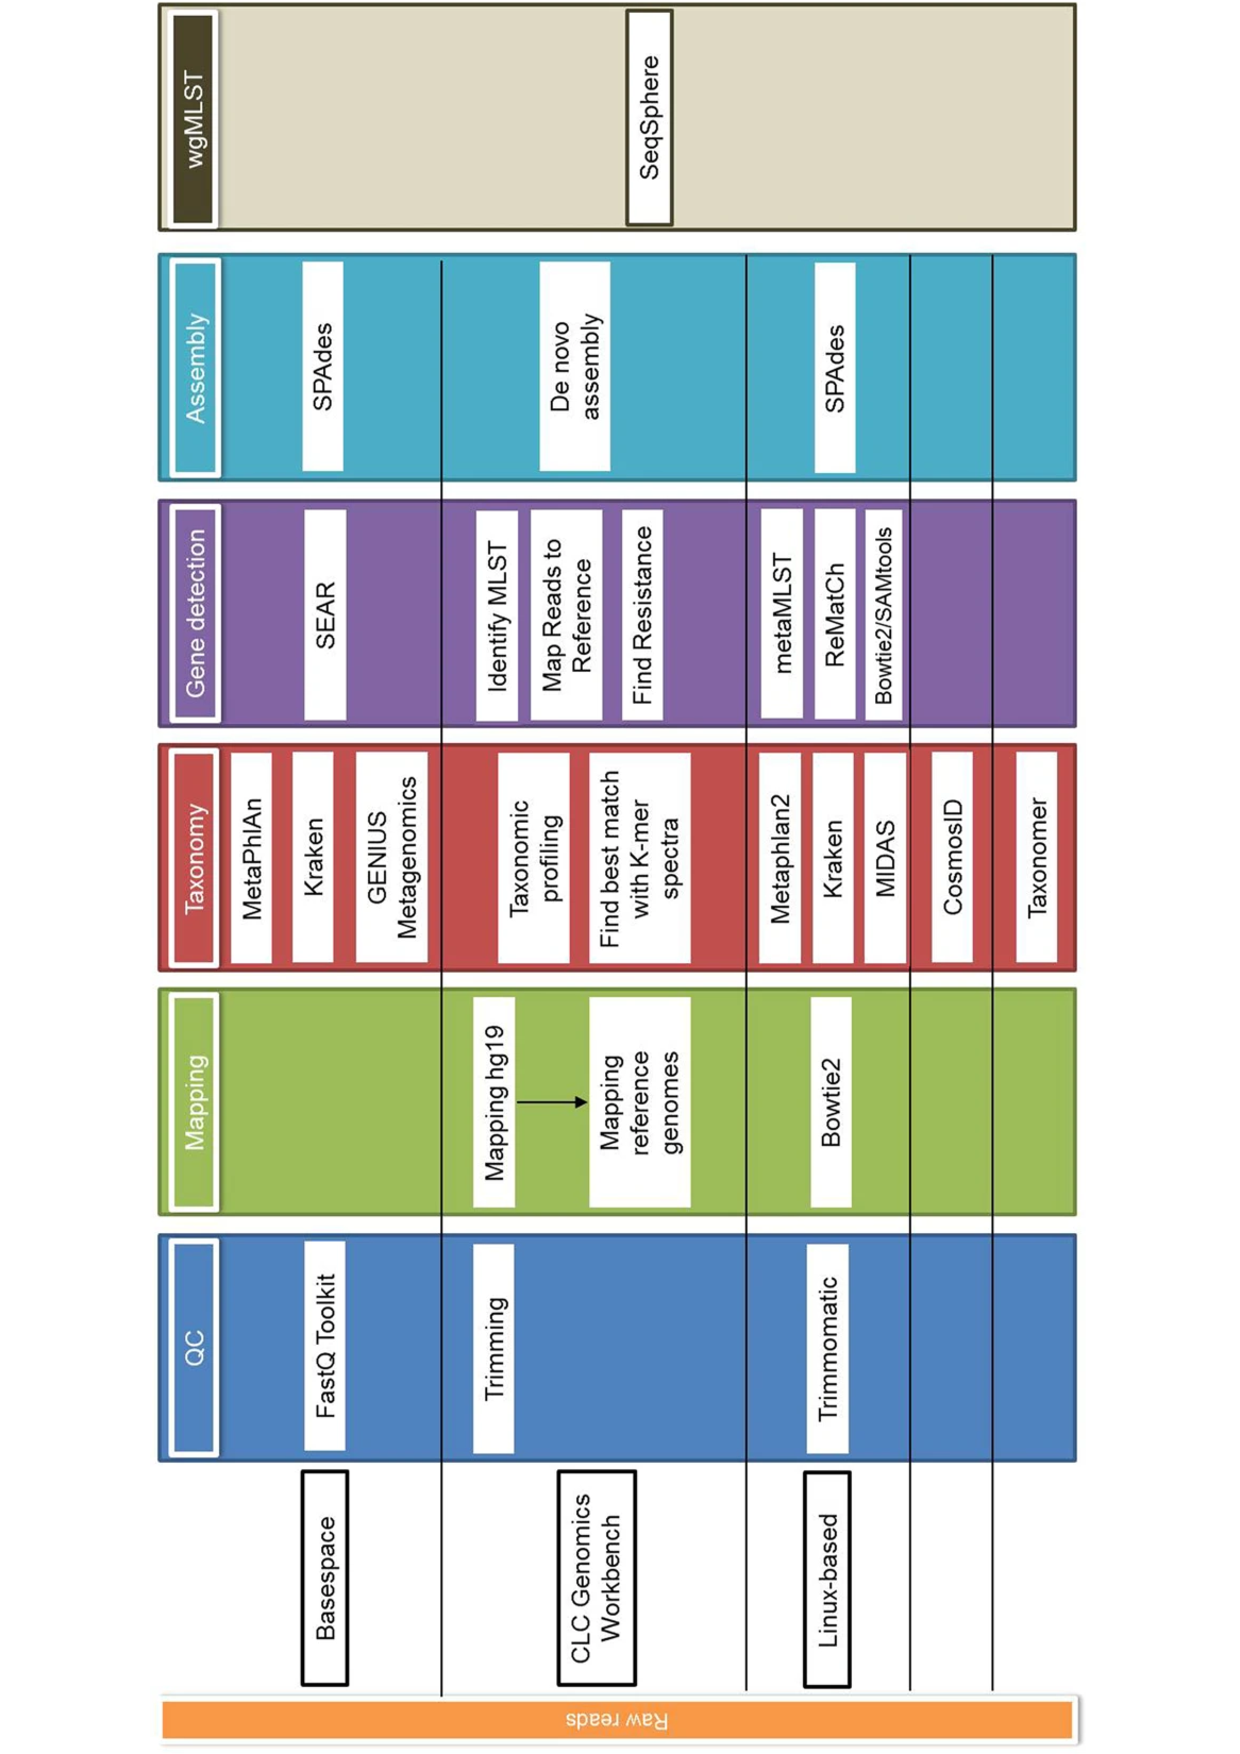
\includegraphics[angle=-90,width=\textwidth]{figures/chapter 2/41598_2018_31873_Fig1_HTML.pdf}
\caption{Scheme of the bioinformatic analysis of the metagenomics samples.}
\label{fig:chap2_figure1}
\end{figure*}

\subsection{Determination of antimicrobial resistance}

Metagenomics provides other sequence information in addition to pathogen detection. 
We determined the presence of antimicrobial-resistance genes in the SMg sequence data and compared the results with those obtained from WGS and phenotypic resistance testing (Table \ref{ch2_table6}).

AMR genes found with CLC Genomics Workbench and ReMatCh in samples 1, 7 and 9 correlated well with phenotypic results. 
However, in the other 7 samples, not all antimicrobial resistance genes that could explain the phenotypic profile were identified. 
In addition, in samples 2, 5, 7 and 10, ReMatCh detected different resistance genes compared to those reported by CLC Genomics Workbench (Table \ref{ch2_table6}).
Some of these differences (genes \textit{norA}, \textit{blaSST}-1, \textit{fusA}) were due to slight differences in the databases used, however, the other resistance genes were present in both databases. 
Interestingly, in two samples (samples 2 and 5), we were able to identify several antimicrobial resistance genes usually found in anaerobic bacteria. 
These were not reported by classical microbiology methods, probably because they were not considered relevant pathogens worthy of subsequent susceptibility study (mixed anaerobic culture).

The SEAR app in BaseSpace (the only one available for antimicrobial resistance gene detection) crashed several times, although we performed the analysis repeatedly, using different parameters.
We were only able to get results in 3 samples, with no resistance genes detected.

\begin{table}[]
\caption{Antimicrobial resistance phenotypes and antimicrobial resistance genes detected using different approaches.}
\label{tab:ch2_table6}
\resizebox{\textwidth}{!}{%
\begin{tabular}{@{}|l|l|l|l|ll|@{}}
\toprule
\multicolumn{1}{|c|}{\multirow{2}{*}{\textbf{Sample number}}} &
  \multicolumn{1}{c|}{\multirow{2}{*}{\textbf{\begin{tabular}[c]{@{}c@{}}Conventional identification\\  (MALDI-TOF)\end{tabular}}}} &
  \multicolumn{1}{c|}{\multirow{2}{*}{\textbf{\begin{tabular}[c]{@{}c@{}}Conventional susceptibility testing\\  (VITEK 2)b\end{tabular}}}} &
  \multicolumn{1}{c|}{\textbf{WGS}} &
  \multicolumn{2}{c|}{\textbf{Shotgun metagenomics}} \\ \cmidrule(l){4-6} 
\multicolumn{1}{|c|}{} &
  \multicolumn{1}{c|}{} &
  \multicolumn{1}{c|}{} &
  \multicolumn{1}{c|}{\textbf{CLC Genomics Workbench}} &
  \multicolumn{1}{c|}{\textbf{ReMatCh (Unix)}} &
  \multicolumn{1}{c|}{\textbf{CLC Genomics Workbencha}} \\ \midrule
\textbf{1} &
  \begin{tabular}[c]{@{}l@{}}E. faecium\\  S. haemolyticus\end{tabular} &
  \begin{tabular}[c]{@{}l@{}}LEV, ERY, CLI\\  OXA, GEN, CIP, FOS, ERY, CLI\end{tabular} &
  \begin{tabular}[c]{@{}l@{}}erm(B), msr(C), ant(6’)-Ia, aph(3’)-III, dfrG\\  blaZ, mecA, ant(6’)-Ia, aph(3’)-III, aac(6’)-aph(2’’), erm(C), mph(C), msr(A), dfrG\end{tabular} &
  \multicolumn{1}{l|}{erm(B), msr(C), ant(6’)-Ia, aph(3’)-III, aac(6’)-aph(2’’), blaZ, mecA, erm(C), mph(C), msr(A), dfrG} &
  erm(B), msr(C), ant(6’)-Ia, aph(3’)-III, aac(6’)-aph(2’’), blaZ, mecA, erm(C), mph(C), msr(A), dfrG \\ \midrule
\textbf{2} &
  \begin{tabular}[c]{@{}l@{}}E. avium\\  E. coli\\  Anaerobes\end{tabular} &
  \begin{tabular}[c]{@{}l@{}}DOX, CLI\\  susceptible\\  -\end{tabular} &
  \begin{tabular}[c]{@{}l@{}}-\#\\  -\#\\  -\#\end{tabular} &
  \multicolumn{1}{l|}{\begin{tabular}[c]{@{}l@{}}Not detected\\  Not detected\\  catS, lnu(D), lsa(C), cepA-44, tet(Q)\end{tabular}} &
  \begin{tabular}[c]{@{}l@{}}Not detected\\  Not detected\\  catS, lnu(D), lsa(C), cepA-44, tet(Q), fusA\end{tabular} \\ \midrule
\textbf{3} &
  S. epidermidis &
  OXA, GEN, TEC, FUS, CIP, ERY, CLI &
  -\# &
  \multicolumn{1}{l|}{Not detected} &
  Not detected \\ \midrule
\textbf{4} &
  S. aureus &
  PEN, ERY &
  blaZ, spc, erm(A) &
  \multicolumn{1}{l|}{Not detected} &
  Not detected \\ \midrule
\textbf{5} &
  \begin{tabular}[c]{@{}l@{}}E. coli\\  K. oxytoca\\  S. anginosus\\  E. faecalis\\  Anaerobes\end{tabular} &
  \begin{tabular}[c]{@{}l@{}}susceptible\\  AMX\\  susceptible\\  DOX, CLI\\  -\end{tabular} &
  \begin{tabular}[c]{@{}l@{}}-\#\\  blaOXY-1-3\\  -\#\\  tet(M), lsa(A)\\  -\#\end{tabular} &
  \multicolumn{1}{l|}{\begin{tabular}[c]{@{}l@{}}-\\  Not detected\\  -\\  tet(M)\\  cfxA4, tet(Q)\end{tabular}} &
  \begin{tabular}[c]{@{}l@{}}-\\  Not detected\\  -\\  tet(O)\\  cfxA4, tet(Q)\end{tabular} \\ \midrule
\textbf{6} &
  E. faecium &
  PEN, AMX, CFX, IMP, GENhl, STRhl, LEV, ERY, CLI, AMP/SUL &
  erm(B), msr(C), ant(6’)-Ia, aph(3’)-III, aac(6’)-aph(2’’), dfrG &
  \multicolumn{1}{l|}{Not detected} &
  Not detected \\ \midrule
\textbf{7} &
  S. aureus &
  PEN &
  blaZ &
  \multicolumn{1}{l|}{blaZ, norA} &
  blaZ \\ \midrule
\textbf{8} &
  O. intermedium &
  AMX, PIP/TAZ, CFX, CFT, CTZ, IMP, FOX, TOB, FOS, NIT, TMP &
  blaOCH-2 &
  \multicolumn{1}{l|}{blaOCH-5} &
  blaOCH-2 \\ \midrule
\textbf{9} &
  S. aureus &
  PEN &
  -\# &
  \multicolumn{1}{l|}{blaZ} &
  blaZ \\ \midrule
\textbf{10} &
  S. marcescens &
  AMX, AMC, CFX, FOX, NIT, POL &
  -\# &
  \multicolumn{1}{l|}{blaSST-1, tet(41), oqxB, aac(6’)-Ic} &
  tet(41), oqxB, aac(6’)-Ic \\ \bottomrule
\end{tabular}%
}
\item $^a$The analysis aborted when the script tried to connect to NCBI
\item $^b$Only non-susceptibility is indicated. \item Abbreviations: AMP/SUL, ampicillin/sulbactam; AMX, amoxicillin; AMC, amoxicillin/clavulanate; CFX, cefuroxime; FOS, fosfomycin; FOX, cefoxitin; CIP, ciprofloxacin; CLI, clindamycin; DOX, doxycycline; ERY, erythromycin; FUS, fusidic acid; GEN, gentamicin; GENhl, gentamicin high-level; LEV, levofloxacin; NIT, nitrofurantoin; PEN, penicillin; POL, polymyxin B; STRhl, streptomycin high-level; TEC, teicoplanin.
\end{table}

\subsection{MLST and wgMLST analysis}
 
In three cases when SMg data covered $\geq$ 93\% of the genome we were able to identify the ST, which corresponded to the one found using WGS of the isolated bacteria using CLC Genomics Workbench (n=2) and metaMLST (n=1). 
These results are summarized in Table \ref{tab:ch2_table7}.
Assembled genomes and metagenomes, were compared by wgMLST analysis using Ridom SeqSphere+. 
Figure \ref{fig:chap2_figure2} shows examples of the allele difference between the genomes obtained through WGS versus the genomes obtained through shotgun metagenomics.

\begin{table}[]
\caption{Results of MLST using by whole genome sequencing and shotgun metagenomics}
\label{tab:ch2_table7}
\resizebox{\textwidth}{!}{%
\begin{tabular}{@{}|l|l|l|ll|@{}}
\toprule
\multicolumn{1}{|c|}{\multirow{2}{*}{\textbf{Sample number}}} &
  \multicolumn{1}{c|}{\multirow{2}{*}{\textbf{\begin{tabular}[c]{@{}c@{}}Conventional identification\\  (MALDI-TOF)\end{tabular}}}} &
  \multicolumn{1}{c|}{\textbf{WGS}} &
  \multicolumn{2}{c|}{\textbf{Shotgun metagenomics}} \\ \cmidrule(l){3-5} 
\multicolumn{1}{|c|}{} &
  \multicolumn{1}{c|}{} &
  \multicolumn{1}{c|}{\textbf{CLC Genomics Workbench v10.1.1}} &
  \multicolumn{1}{c|}{\textbf{CLC Genomics Workbench v10.1.1}} &
  \multicolumn{1}{c|}{\textbf{metaMLST (Unix-based)}} \\ \midrule
\textbf{1} &
  \begin{tabular}[c]{@{}l@{}}\textit{E. faecium}\\  \textit{S. haemolyticus}\end{tabular} &
  \begin{tabular}[c]{@{}l@{}}ST117\\  ST25\end{tabular} &
  \multicolumn{1}{l|}{\begin{tabular}[c]{@{}l@{}}Not detected (6 alleles identified correctly)\\  Not detected (3 alleles identified correctly)\end{tabular}} &
  \begin{tabular}[c]{@{}l@{}}ST117\\  Not detected\end{tabular} \\ \midrule
\textbf{2} &
  \begin{tabular}[c]{@{}l@{}}\textit{E. avium}\\  \textit{E. coli}\\  Anaerobes\end{tabular} &
  \begin{tabular}[c]{@{}l@{}}-$^\#$ \\  -$^\#$ \\  -$^\#$ \end{tabular} &
  \multicolumn{1}{l|}{\begin{tabular}[c]{@{}l@{}}-\\  Not detected\\  -\end{tabular}} &
  \begin{tabular}[c]{@{}l@{}}-\\  Not detected\\  -\end{tabular} \\ \midrule
\textbf{3} &
  \textit{S. epidermidis} &
  -$^\#$ &
  \multicolumn{1}{l|}{Not detected} &
  Not detected \\ \midrule
\textbf{4} &
  \textit{S. aureus} &
  ST30 &
  \multicolumn{1}{l|}{Not detected} &
  Not detected \\ \midrule
\textbf{5} &
  \begin{tabular}[c]{@{}l@{}}\textit{E. coli}\\  \textit{K. oxytoca}\\  \textit{S. anginosus}\\  \textit{E. faecalis}\\  Anaerobes\end{tabular} &
  \begin{tabular}[c]{@{}l@{}}ST141\\  ST40\\  -$^\#$ \\  ST179\\  -$^\#$ \end{tabular} &
  \multicolumn{1}{l|}{\begin{tabular}[c]{@{}l@{}}ST141\\  Not detected\\  -\\  Not detected\\  -\end{tabular}} &
  \begin{tabular}[c]{@{}l@{}}ST4508\\  Not detected\\  -\\  Not detected\\  -$^\#$ \end{tabular} \\ \midrule
\textbf{6} &
 \textit{ E. faecium} &
  ST117 &
  \multicolumn{1}{l|}{Not detected} &
  Not detected \\ \midrule
\textbf{7} &
  \textit{S. aureus} &
  ST30 &
  \multicolumn{1}{l|}{ST30} &
  ST667 \\ \midrule
\textbf{8} &
  \textit{O. intermedium} &
  - &
  \multicolumn{1}{l|}{-} &
  - \\ \midrule
\textbf{9} &
  \textit{S. aureus} &
  -$^\#$  &
  \multicolumn{1}{l|}{Not detected} &
  Not detected \\ \midrule
\textbf{10} &
  \textit{S. marcescens} &
  -$^\#$ &
  \multicolumn{1}{l|}{-} &
  - \\ \bottomrule
\end{tabular}%
}
\item Abbreviations: ST, sequence type
\end{table}

\begin{figure*}[h!]
\centering
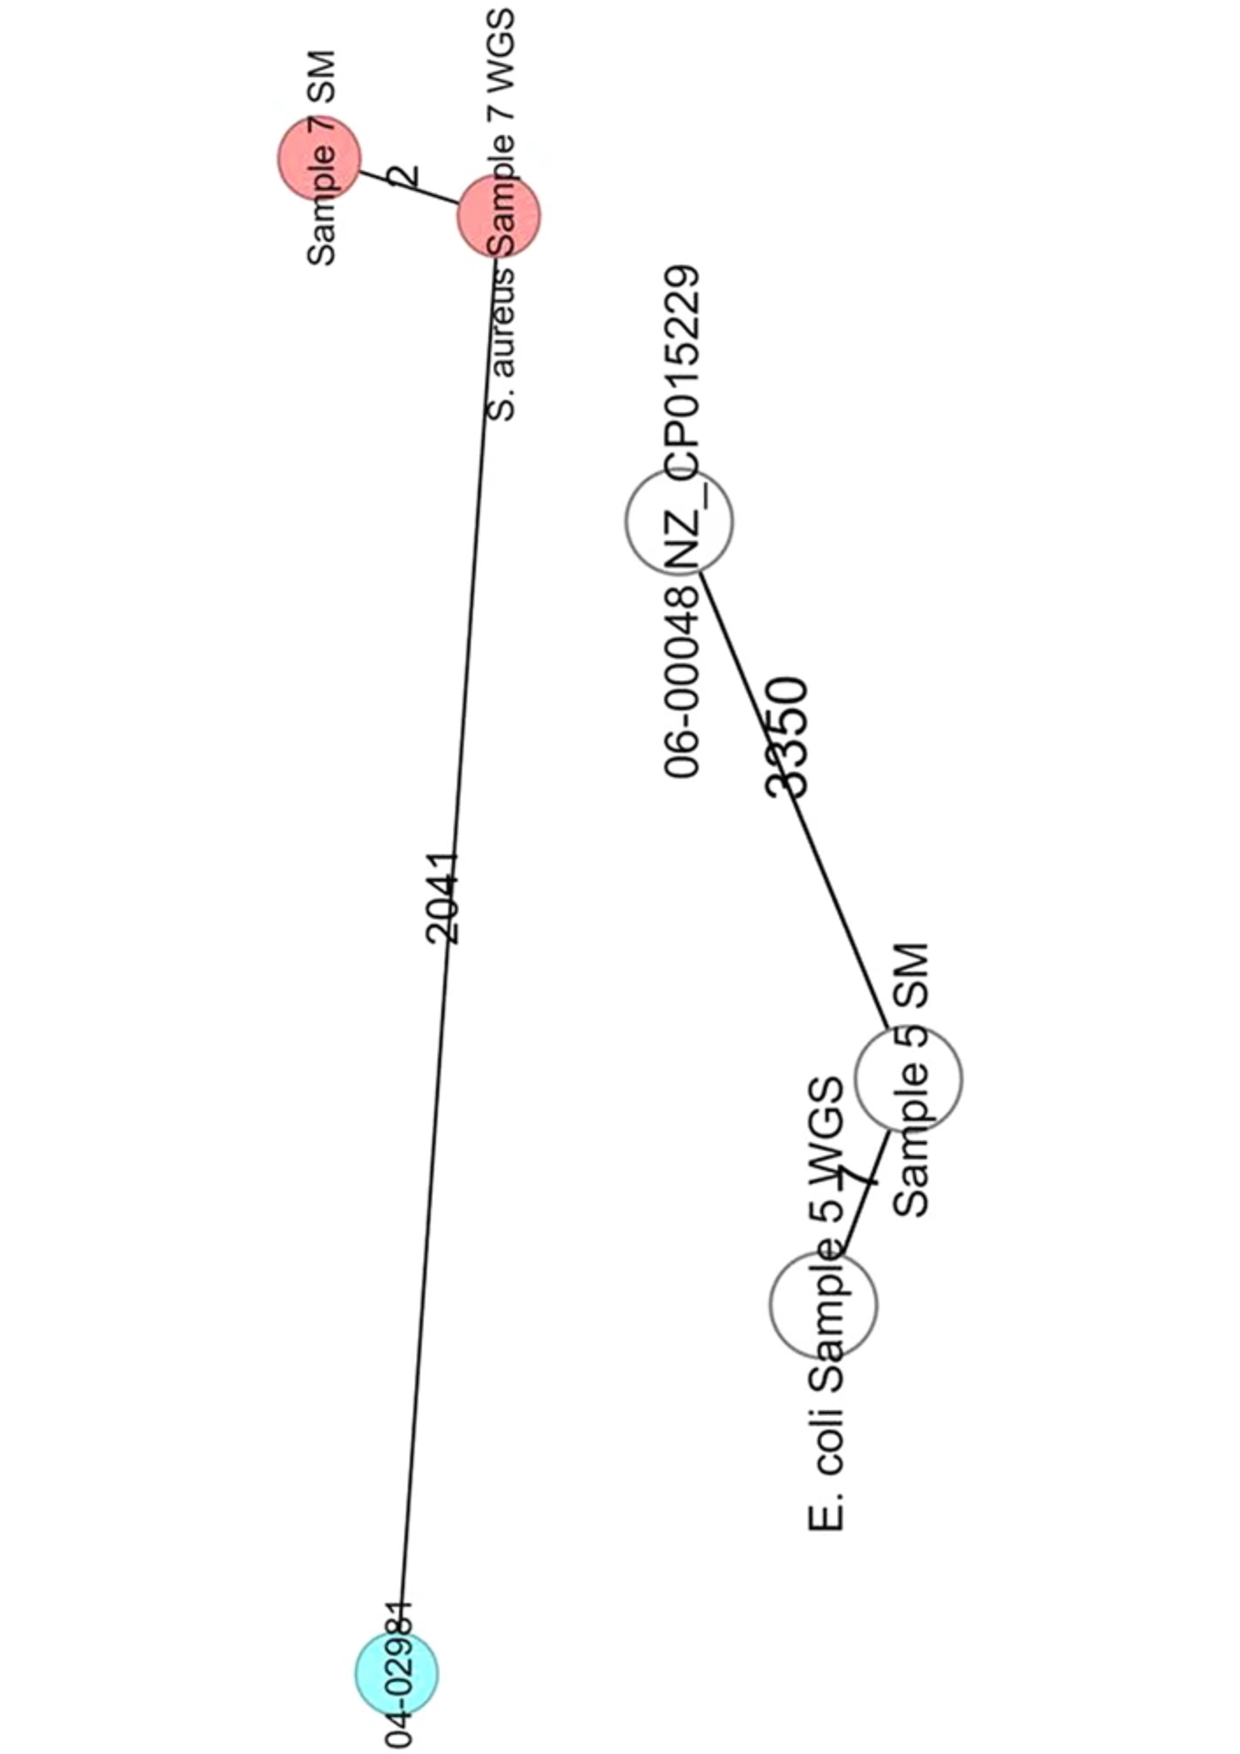
\includegraphics[angle=-90,width=\textwidth]{figures/chapter 2/41598_2018_31873_Fig2_HTML.pdf}
\caption{Minimum-spanning tree based on wgMLST allelic profiles of 2 S. aureus genomes and 2 E. coli genomes obtained through SM and WGS in comparison to reference strains 04-02981 (GenBank accession number NC\_017340) and 06-00048 (NZ\_CP015229), respectively. Each circle represents an allelic profile based on sequence analysis. The numbers on the connecting lines illustrate the numbers of target genes with differing alleles.}
\label{fig:chap2_figure2}
\end{figure*}

\subsection{Characterisation of mobile genetic elements}

Two different approaches, i.e. CLC Genomics Workbench and Bowtie2 were used to identify plasmids present in the sequence data. 
Both approaches used mapping of sequences against the same plasmid database. 
Since some plasmids present in the database are very similar and sequence reads may be mapped to more than one plasmid, we used the pATLAS tool, which provides an overview of the nodes (representing plasmid sequences) and links between plasmids (which connect similar plasmids), to enable the visualisation of the plasmids identified (Figure \ref{fig:chap2_figure3}). 
A colour gradient indicates the sequence coverage of the plasmids. 
In most cases, the same plasmids were identified by both approaches, with some small differences in sequence coverage. 
When comparing the plasmids identified in the SMg dataset versus the WGS data, most of the plasmids were also detected in the isolates (an example is shown in Figure \ref{fig:chap2_figure4}). 
However, some plasmids were not identified in any of the isolated bacteria and were probably residing in low-abundant species.

\begin{figure*}[h!]
\centering
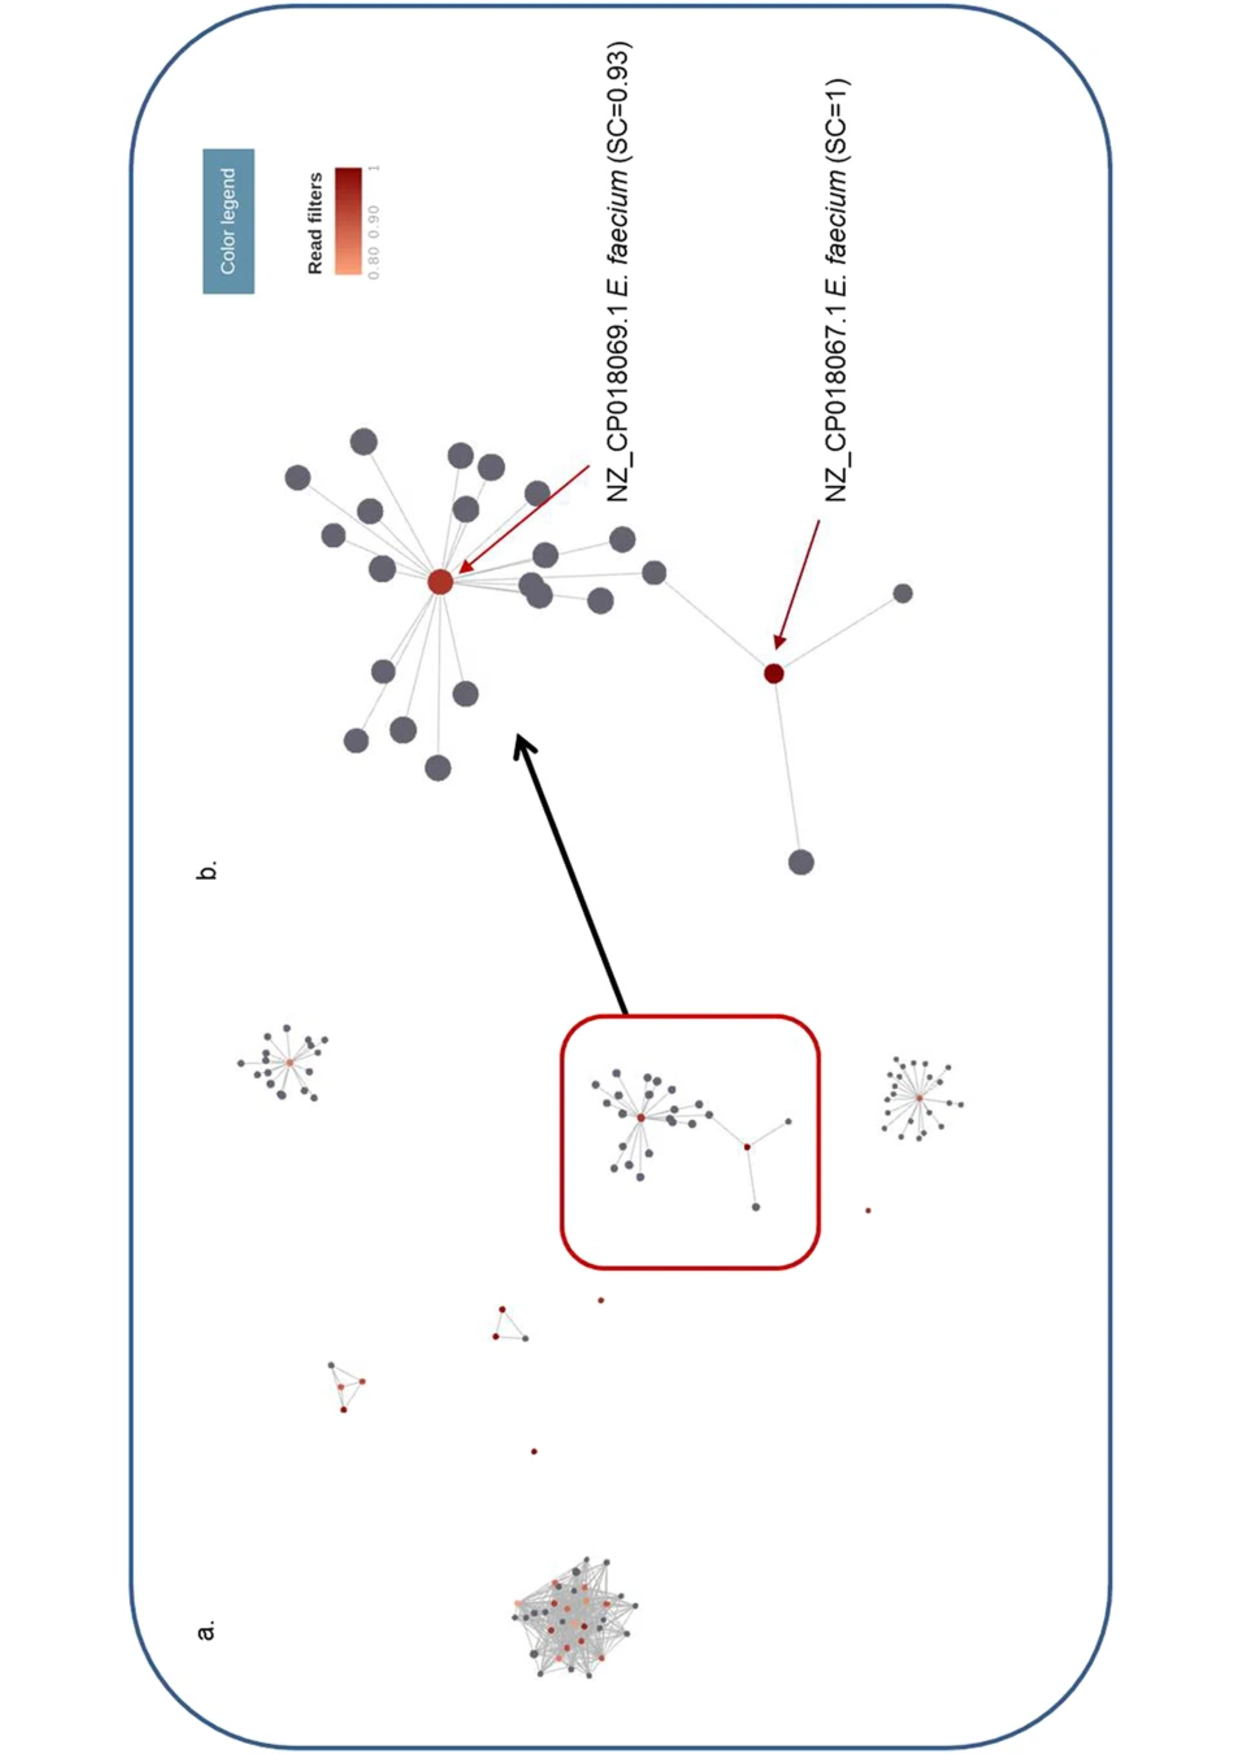
\includegraphics[angle=-90,width=\textwidth]{figures/chapter 2/41598_2018_31873_Fig3_HTML.pdf}
\caption{(a) Overview of the nodes (representing plasmid sequences) and links between plasmids (connecting similar plasmids) found in Sample 1 (SMg) using the pATLAS tool. (b) A closer look at one of the cloud of plasmids. The colour gradient in each cloud of plasmids represents the plasmid sequence coverage (SC), varying between 0-0.79 (grey) and 0.80-1 (red gradient).}
\label{fig:chap2_figure3}
\end{figure*}

\begin{figure*}[h!]
\centering
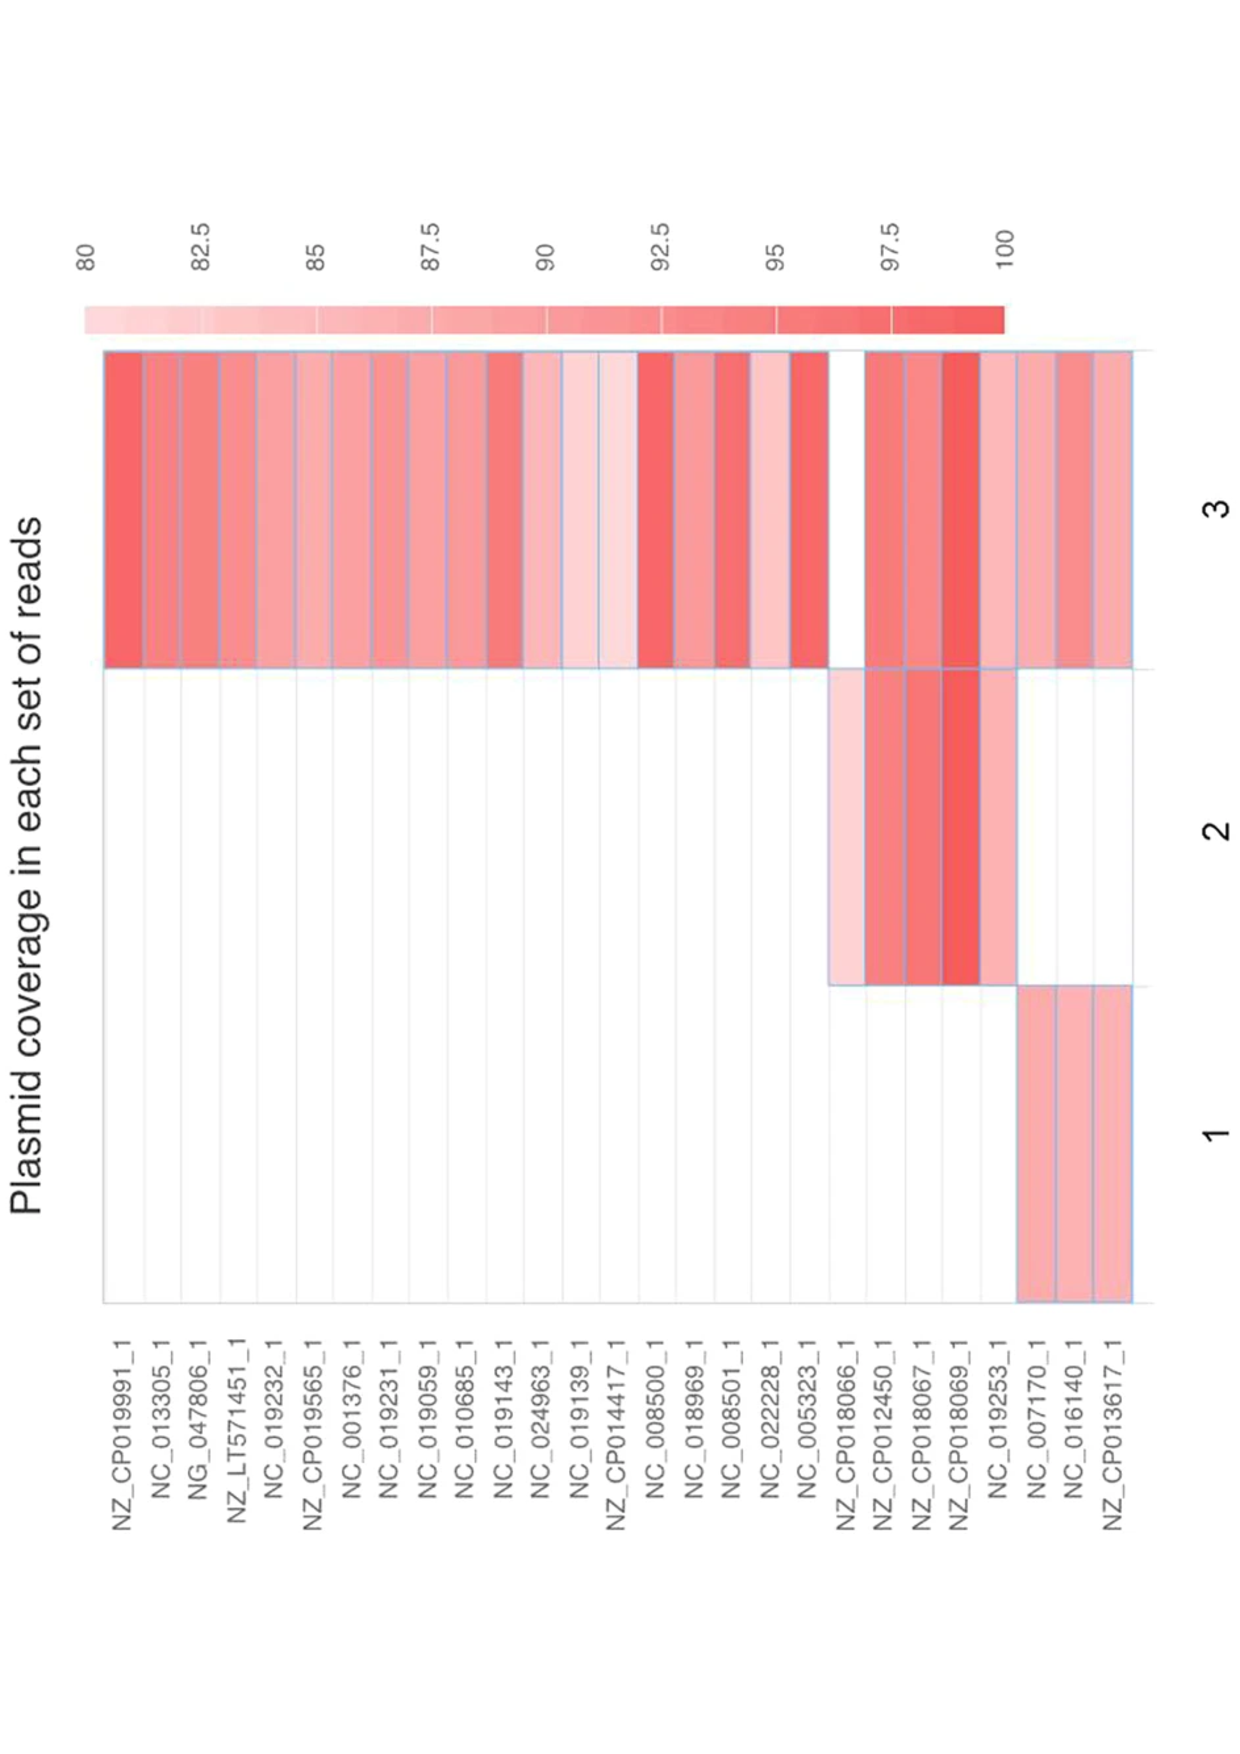
\includegraphics[angle=-90,width=\textwidth]{figures/chapter 2/41598_2018_31873_Fig4_HTML.pdf}
\caption{A heatmap comparing the identified plasmids using bowtie2 in \textit{S. haemolyticus} WGS (1),\textit{ E. faecium} WGS (2) and in the SMg dataset (3) isolated from sample 1.}
\label{fig:chap2_figure4}
\end{figure*}

\section{Discussion}

This study evaluated the suitability of SMg for the microbiological diagnosis and (patho- and epi-) typing of microorganisms directly from real patient samples. The whole procedure took between 48-54 hours to complete, which is shorter than culture-based methods if one includes typing. However, the amount of information derived from SMg in most cases, did not overcome the necessity for pathogen isolation and subsequent (phenotypic and genotypic) typing, which can take up to 1-2 weeks (particularly in slow-growing organisms). Nevertheless, SMg can help guide antimicrobial therapy and be helpful in cases where there is a suspicion of transmission and there is a need to quickly determine the genetic relationship between pathogens, although the success of SMg in individual patient samples can be highly variable, as reported here.

Different bioinformatics pipelines were evaluated to identify potential differences between them and identify those which could provide the clinical microbiologist with the maximum of relevant and accurate information. In terms of microbial identification, in both Unix and web-based approaches we would recommend MetaPhlAn, since it has good sensitivity and a good positive predictive value (PPV). The find best match K-mer spectra tool should be used in the context of the CLC Genomics Workbench, since it had a higher sensitivity and PPV compared to the Taxonomic Profiling tool.

In a clinical setting, a combination of high sensitivity and high PPV of any new method is key. Popular software designed for bacterial identification, can predict dozens to hundreds of species in in vitro generated bacterial communities of known composition \citep{peabody_evaluation_2015}. We observed the same when using Kraken and Taxonomer when comparing to culture-based methods. For both Kraken and Taxonomer, relative abundance cut-off values may be required to limit the number of species identified. However, which cut-off values should be used are a matter of debate, since in some cases, even if applying a cut-off value as low as 1.0\% (comparable to what was found in the negative control) would have resulted in decreased sensitivity (e.g. the \textit{Streptococcus anginosus} identified by culture in Sample 5 would have been disregarded). The methods that employ several parameters to infer microbial identification are superior, because they not only rely on the relative abundance of bacterial species, but also on the genome coverage and on the proportion of the genome that was covered. On the other hand, in some cases SMg may be more sensitive than culture in identifying pathogens, reflecting the higher sensitivity or the capacity to detect bacterial species which are non-culturable in the conditions used or that are no longer culturable, such as due to prior antimicrobial therapy. In such cases, other methods like 16S rDNA sequencing or the recently described 16S-23S rDNA sequencing method \citep{sabat_targeted_2017} may be used for discrepancy analyses. However, here we decided to use culture-based methods as the gold standard, since this is still the method of choice in clinical microbiology.

One limitation of this study was the exclusion of culture-negative samples and thus their inclusion would have affected the calculation of the specificity values. However, as mentioned above, culture-negative samples do not necessarily mean that the samples are pathogen-free, but it might only reflect the low sensitivity or capacity of culture-based methods to detect non-culturable bacterial species. As with other (molecular) methods, several controls should be included to validate the obtained results, including a negative control. In our negative control, we detected an \textit{O. intermedium} strain, although with only 1.0\% of the reads mapping to the reference genome and covering only 1.4\% of the reference genome (accession number NZ\_ACQA01000002). These results may be due to contamination during library preparation (e.g. sample-to-sample contamination prior to indexing), the result of sequencing artefacts (e.g. demultiplexing errors), or to incorrect classification during data analysis (e.g. highly similar regions) \citep{graf_unbiased_2016}. Our samples and sequencing libraries were handled in laminar flow cabinets; however, we cannot also exclude the possibility of contamination. Furthermore, the reagents used may also be or become contaminated with DNA leading the detection of these contaminating species, something that has been described previously \citep{street_molecular_2017}. This poses a challenge for interpretation, because some positive samples also had very low numbers of reads for some pathogens (< 1\%). When approaching this limit of detection, small numbers of pathogen reads will be difficult to interpret, as they can represent true-positives with low abundance in the sample, or artefacts such as contamination during library preparation\citep{graf_unbiased_2016}.

In terms of antimicrobial resistance gene detection, ReMatCh (Unix) and the CLC Genomics Workbench Find Resistance tool gave comparable results. Since ReMatCh (Unix) performs the analysis at the read level, while CLC Genomics Workbench performs it at the contig level, we suggest that both strategies should be employed in parallel when looking for antimicrobial resistance genes. It is also important to emphasise that the contig-level approach employed by CLC Genomics Workbench may give negative results if the sequence coverage is set to a high percentage (e.g. above 80\%). This is due to the assembly method, which may split the antimicrobial resistance genes into different contigs, when the number of reads is too low. This phenomenon was observed in Sample 1, for the \textit{aac(6’)-aph(2’’)} gene, which was split into 3 different contigs, each part corresponding to less than 40\% of the gene. Only when applying a cut-off value of $geq$ 20\% for sequence coverage could we identify all three parts of the gene, which in total corresponded to 89\% of the entire sequence. Finally, it is important to point out that the ResFinder database (used here), and other databases, focus on acquired genes, not including chromosomal point mutations resulting in antimicrobial resistance. However, a recently developed tool, PointFinder, was added to ResFinder for the detection of chromosomal point mutations associated with antimicrobial resistance \citep{zankari_pointfinder_2017} and an updated database will be available soon.

Another challenge is to infer where these antimicrobial resistance genes are located (chromosome or plasmid). The study of mobile genetic elements, including plasmids, carrying antimicrobial resistance genes present in clinical samples is important to predict possible treatment failures and the spread of resistance within and across bacterial species. When performing bacterial isolation followed by WGS, information on polymicrobial infections may be lost. This is mainly driven by a bottleneck in culture, where some bacterial species are not isolated with standard work up protocols (frequently anaerobes and slow-growing organisms). The presence of antimicrobial resistance genes in plasmids of bacteria other than those isolated through culture poses a risk since they are not identified by conventional methods but could potentially be horizontally transmitted to pathogenic bacteria under the antimicrobial selective pressure of treatment. Antimicrobial administration may also select minority populations where these resistance determinants are found. Furthermore, the understanding of how plasmids are shared by different bacteria in a bacterial community (e.g. within an infection site or in the gut) can improve our understanding of how these elements disseminate across species and from patient to patient11. The SMg approach is clearly more efficient than culture in identifying the “cloud” of plasmids present in a given sample (Figure 4) and which can be potentially transferred to more pathogenic species generating problems of resistance, as was the case with the emerge of vancomycin resistance \textit{S. aureus} \citep{melo-cristino_first_2013}.

Whole-genome sequencing has been used extensively for several purposes \citep{deurenberg_application_2017} and is considered to have the potential of playing an important role in clinical microbiology \citep{rossen_practical_2018}. It is the ongoing goal of medical molecular microbiology to develop faster typing methods that can be used for outbreak surveillance. For this purpose, we assembled the metagenomics data and compared it with the assemblies given by WGS. Surprisingly, the assemblies provided by SPAdes in BaseSpace were closer to the assemblies provided by WGS. When comparing the genomes obtained through WGS and SMg, we could see that in 4 out of 8 bacterial isolates the number of different alleles was $leq$ 7. This showed the potential of SMg to draw phylogenetic relationships from uncultured bacterial genomes, although more potentially limited than those obtained using WGS data from axenic cultures. As for the detection of resistance genes, a key limiting factor may be the number of bacterial reads, reflected in a lower genome coverage (e.g. samples 4 and 6). In these cases, we would have to either improve the human-DNA depletion step, improve the microbial enrichment or perform sequencing at a higher sequencing depth to have enough microbial reads to be able to get a more appropriate genome coverage. Yet, this last step will severely raise the sequencing costs, which might render the methodology unfeasible for routine application.

In this study, we evaluated the results of metagenomics pipelines using three different methods. CLC Genomics Workbench has advantages over the other methods. It does not require previous knowledge of Unix-based tools, it is arguably the most user-friendly and delivered reliable results for microbial identification and antimicrobial resistance gene detection. The downside was the assembly approaches, which provided lower wgMLST allele detection, when compared to the assemblies using SPAdes (BaseSpace and Unix). BaseSpace, the other commercial solution, on the other hand, provided only a few tools that can be used for metagenomics data. Furthermore, since Illumina did not develop the apps themselves, they offered no direct support. Contacting the developers (via email and posting on their forum) does not guarantee a solution to the issues in a time frame compatible with a routine clinical microbiology laboratory work. The dependence and no direct control over a third party to resolve software bugs and provide a stable platform illustrates a disadvantage of a cloud-based system like BaseSpace. Finally, the Unix-based pipeline complemented the data on antimicrobial resistance genes but did not offer better results in terms of microbial identification and MLST typing. However, many more freely available tools for this last purpose could have been used, potentially improving on the results obtained. Reference-guided assembly approaches, taking advantage of the species information derived in the first steps of our analysis pipelines, will deserve further study in the future since these may provide higher quality assemblies from metagenomics data. The main advantage of an open-source approach is its flexibility since it allows the user to choose the most adequate method for each desired outcome.
There were several limitations to this study. First, the number of samples included was low and some of the bacterial isolates were not available for further WGS analysis. However, the extended data analyses performed in each sample limited the number of samples to be included. It is our intention to move forward with the most adequate pipelines for each purpose and apply them to additional patients’ samples. Second, the samples differed greatly from each other. However, in our point of view, this was beneficial to the study, since it did not bias the analyses as it could have happened if only one type of sample had been used. Finally, we used three different extraction methods that could have influenced the final results. Yet, as can be seen in Table 1, the number of human reads differed between samples, even when using the same extraction kit. This suggests none of the kits is clearly superior to the others and that the ratio between host and microbial DNA or other individual sample characteristics will be the major determinants of the proportion of microbial reads.

In conclusion, this study showed the potential but also highlighted the problems of implementing shotgun metagenomics for the identification and typing of pathogens directly from clinical samples. Based on the results obtained here we can conclude that the tools and databases used for taxonomic classification and antimicrobial resistance will have a key impact on the results, cautioning about the comparison between studies using different methods and suggesting that efforts need to be directed towards standardisation of the analysis methods if SMg is to be used routinely in clinical microbiology.

\section{Acknowledgements}

We thank Peter Posma, Yvette Bisselink and Brigitte Dijkhuizen for excellent technical assistance. We thank Dr. Michael Lustig and colleagues from Molzym Life Science for helping with extraction protocols.

This project has received funding from the European Union’s Horizon 2020 research and innovation program under the Marie Skłodowska-Curie grant agreement 713660.This work was partly supported by the INTERREG VA (202085) funded project EurHealth-1Health, part of a Dutch-German cross-border network supported by the European Commission, the Dutch Ministry of Health, Welfare and Sport (VWS), the Ministry of Economy, Innovation, Digitalisation and Energy of the German Federal State of North Rhine-Westphalia and the German Federal State of Lower Saxony.

\section{Author contributions statement}

N.C., J.A.C., M.R., S.P., I.A., A.W.F. and J.W.A conceived the experiment(s), N.C., L.S. and E.C.R. conducted the experiment(s), N.C., L.S., M.M., C.I.M., T.F.J., S.R., M.C., J.A.C. and M.R. analysed the results, N.C. and L.S. wrote the manuscript. All authors reviewed the manuscript.

\section{Additional information}

\subsection{Accession codes} \label{ch2_supmaterial}

The paired-trimmed-un-mapped reads (hg19) generated for each sample have been submitted to SRA under project number SRP126380. 
The cgMLST schemes are deposited in figshare under the DOI:10.6084/m9.figshare.5679376

\subsection{Competing financial interests}

The authors declare that they have no conflict of interest.

\section{Supplemental Material}

\begin{table}[]
\caption{}
\label{tab:ch2_suptable1}
\resizebox{\textwidth}{!}{%
\begin{tabular}{ll}
\multicolumn{2}{c}{\textbf{FastQ Toolkit v2.2.0}}                                       \\
Minimum read length                             & 32                           \\
Sub-sampling                                    & FALSE                        \\
Adapter trim stringency                         & 0.9                          \\
Select respective adapters                      & TRUE                         \\
Quality trimming                                & FALSE                        \\
Poly-A/T Trimming                               & FALSE                        \\
Read Filtering                                  & FALSE                        \\
Modify Reads                                    & FALSE                        \\
Fix Format                                      & FALSE                        \\
\multicolumn{2}{c}{\textbf{FastQC v1.0.0}}                                              \\
Kmer Size                                       & 5                            \\
Use Conatminant Filter                          & TRUE                         \\
\multicolumn{2}{c}{\textbf{Kraken Metagenomics v1.0.0}}                                 \\
Host Filter                                     & TRUE RefSeqhg19              \\
Classification Database                         & MiniKraken 20141208 (latest) \\
Filter Threshold                                & 0                            \\
\multicolumn{2}{c}{\textbf{Metaphlan v1.0.0}}                                           \\
Sensitivity options for read-marker similarity (as descibed by BowTie2)                  & Very Sensitive \\
\multicolumn{2}{c}{\textbf{SPAdes Genome Assembler v3.9.0}}                             \\
Running Mode                                    & Error Correction \& Assembly \\
Dataset type                                    & Multi Cell                   \\
Careful Mode                                    & Disable                      \\
k-mer lengths                                   & Auto                         \\
\multicolumn{2}{c}{\textbf{SEAR: Antibiotic Resistance v1.0.0}}                                           \\
Read length cutoff (bases)                      & 70                           \\
Read quality score cutoff                       & 20                           \\
Read subtraction against E.coli reference genome (K12)?                                  & No             \\
Clustering stringency (express \% as a decimal) & 0.98                         \\
Annotation stringency (\% length of reference ARG sequence mapped to by sequencing reads & 40             \\
\multicolumn{2}{c}{\textbf{GENIUS Metagenomics: Know Now v1.1.0}}                                                  \\
Can't set any settings in BaseSpace             &                             
\end{tabular}%
}
\end{table}

\begin{table}[]
\caption{}
\label{tab:ch2_suptable2}
\resizebox{\textwidth}{!}{%
\begin{tabular}{ll}
\multicolumn{2}{l}{Trim Reads}                                                          \\
Trimmomatic v0.36 (INNUca v2.6 initial module)     &                                    \\
Quality trim                                       & TRUE                               \\
Phred Quality limit                                & 05:20                              \\
Trim adapter list                                  & Illumina adapters                  \\
Remove 5' terminal nucleotides                     & TRUE                               \\
Number of 5' terminal nucleotides                  & 3                                  \\
Remove 3' terminal nucleotides                     & TRUE                               \\
Number of 3' terminal nucleotides                  & 3                                  \\
Discard short reads                                & TRUE                               \\
Minimum number of nucleotides in reads             & 55                                 \\
                                                   &                                    \\
\multicolumn{2}{l}{Map Reads to Reference}                                              \\
Bowtie2 v2.3.2                                     &                                    \\
References                                         & Homo sapiens (hg19) index          \\
Mode                                               & end-to-end                         \\
Mode option                                        & sensitive                          \\
Collect unmapped reads                             & FALSE                              \\
                                                   &                                    \\
\multicolumn{2}{l}{Taxonomic classification}                                            \\
Kraken v0.10.5-beta                                &                                    \\
References                                         & miniKraken database (Dec. 8, 2014) \\
K-mer length                                       & 35                                 \\
MIDAS                                              &                                    \\
References                                         & midas\_db\_v1.2 (May 9, 2018)      \\
Word size for blast                                & 28                                 \\
Alignment coverage                                 & 0.75                               \\
MetaPhlAn2 v2.0                                    &                                    \\
References                                         & default database (May 9, 2018)     \\
Minimum total nucleotide length for the markers    & 2000                               \\
Quantile value for robust average                  & 0.1                                \\
Statistical approach for converting marker abundances into clade abundances & clade global                                          \\
Analysis type                                                               & profiling a metagenome in terms of relative abundance \\
                                                   &                                    \\
\multicolumn{2}{l}{Identify MLST}                                                       \\
metaMLST v1.1                                      &                                    \\
References                                         & metamlstDB\_2017                   \\
Bowtie2 mode                                       & local                              \\
Bowtie2 mode option                                & very sensitive local               \\
Collect unmapped reads                             & FALSE                              \\
Search for and report all alignment                & TRUE                               \\
                                                   &                                    \\
\multicolumn{2}{l}{Find Resistance Genes}                                               \\
ReMatCh v3.2                                       &                                    \\
References                                         & ResFinder database (29-06-2017)    \\
Minimum coverage to consider a position as present & 1                                  \\
Minimum coverage depth to perform a basecall       & 1                                  \\
Minimum gene coverage (\%)                         & 80                                 \\
Minimum gene identity (\%)                         & 70                                 \\
                                                   &                                    \\
\multicolumn{2}{l}{De novo assembly}                                                    \\
SPAdes v3.10.1                                     &                                    \\
Mode                                               & careful                            \\
Error correction                                   & FALSE                              \\
Read coverage cut-off value                        & 2                                  \\
List of K-mers                                     & 21,33,55,67,77                     \\
                                                   &                                    \\
\multicolumn{2}{l}{Plasmid Detection}                                                   \\
Bowtie2 v2.3.2                                     &                                    \\
References                                         & NCBI RefSeq (May 11, 2017)         \\
Mode                                               & end-to-end                         \\
Mode option                                        & sensitive                          \\
Collect unmapped reads                             & FALSE                              \\
Multiple alignment                                 & TRUE                              
\end{tabular}%
}
\end{table}

\newpage

\begin{longtable}{ll}
\caption{}
\label{tab:ch2_suptable3}\\
\multicolumn{2}{l}{Illumina}                                                                  \\
\endfirsthead
%
\endhead
%
Discard sequence names                       & FALSE                                          \\
Discard quality scores                       & FALSE                                          \\
Selected files                               &                                                \\
Paired-end reads                             & TRUE                                           \\
Read Orientation                             & Forward Reverse                                \\
minimum distance                             & 1                                              \\
maximum distance                             & 1000                                           \\
Remove failed reads                          & TRUE                                           \\
Quality score                                & NCBI/Sanger or Illumina Pipeline 1.8 and later \\
MiSeq de-multiplexing                        & FALSE                                          \\
Illumina trim                                & FALSE                                          \\
                                             &                                                \\
Trim Reads                                   &                                                \\
Quality trim                                 & TRUE                                           \\
Quality limit                                & 0.05                                           \\
Ambiguous trim                               & TRUE                                           \\
Ambiguous limit                              & 2                                              \\
Trim adapter list                            & Illumina adapters                              \\
Use colorspace                               & FALSE                                          \\
Remove 5' terminal nucleotides               & FALSE                                          \\
Number of 5' terminal nucleotides            & 1                                              \\
Remove 3' terminal nucleotides               & FALSE                                          \\
Number of 3' terminal nucleotides            & 1                                              \\
Discard short reads                          & TRUE                                           \\
Minimum number of nucleotides in reads       & 30                                             \\
Discard long reads                           & FALSE                                          \\
Maximum number of nucleotides in reads       & 1000                                           \\
                                             &                                                \\
Map Reads to Reference                       &                                                \\
References                                   & Homo sapiens (hg19) sequence                   \\
Masking mode                                 & No masking                                     \\
Masking track                                &                                                \\
Match score                                  & 1                                              \\
Mismatch cost                                & 2                                              \\
Cost of insertions and deletions             & Linear gap cost                                \\
Insertion cost                               & 3                                              \\
Deletion cost                                & 3                                              \\
Insertion open cost                          & 6                                              \\
Insertion extend cost                        & 1                                              \\
Deletion open cost                           & 6                                              \\
Deletion extend cost                         & 1                                              \\
Length fraction                              & 0.5                                            \\
Similarity fraction                          & 0.8                                            \\
Global alignment                             & FALSE                                          \\
Color space alignment                        & TRUE                                           \\
Color error cost                             & 3                                              \\
Auto-detect paired distances                 & TRUE                                           \\
Non-specific match handling                  & Map randomly                                   \\
                                             &                                                \\
\multicolumn{2}{l}{Find Best Matches using K-mer Spectra}                                     \\
References                                   & NCBI references (2017-07-08)                   \\
K-mer length                                 & 16                                             \\
Only index k-mers with prefix                & ATGAC                                          \\
Check for low quality and contamination      & TRUE                                           \\
Fraction of unmapped reads for quality check & 0.1                                            \\
                                             &                                                \\
De Novo Assembly                             &                                                \\
Mapping mode                                 & Create simple contig sequences (fast)          \\
Update contigs                               & TRUE                                           \\
Mismatch cost                                & 2                                              \\
Insertion cost                               & 3                                              \\
Deletion cost                                & 3                                              \\
Colorspace error cost                        & 3                                              \\
Length fraction                              & 0.5                                            \\
Similarity fraction                          & 0.8                                            \\
Colorspace alignment                         & TRUE                                           \\
Alignment mode                               & local                                          \\
Match mode                                   & random                                         \\
Create list of un-mapped reads               & FALSE                                          \\
Automatic bubble size                        & TRUE                                           \\
Bubble size                                  & 50                                             \\
Automatic word size                          & TRUE                                           \\
Word size                                    & 20                                             \\
Minimum contig length                        & 200                                            \\
Guidance only reads                          &                                                \\
Perform scaffolding                          & TRUE                                           \\
Auto-detect paired distances                 & TRUE                                           \\
Create report                                & TRUE                                           \\
                                             &                                                \\
\multicolumn{2}{l}{Find Resistance}                                                           \\
DB                                           & Database for Find Resistance (2018-02-02)      \\
Minimum identity \%                          & 70                                             \\
Minimum length \%                            & 20                                             \\
Filter overlaps                              & TRUE                                           \\
Local Realignment                            &                                                \\
Realign unaligned ends                       & TRUE                                           \\
Multi-pass realignment                       & 2                                              \\
Guidance-variant track                       &                                                \\
Maximum guidance-variant length              & 100                                            \\
Force realignment to guidance-variants       & FALSE                                          \\
                                             &                                                \\
InDels and Structural Variants (2)           &                                                \\
P-Value threshold                            & 1.00E-04                                       \\
Maximum number of mismatches                 & 3                                              \\
Ignore broken pairs                          & TRUE                                           \\
Filter variants                              & FALSE                                          \\
Minimum number of reads                      & 2                                              \\
Minimum relative consensus coverage          & 0                                              \\
Minimum quality score                        & 0                                              \\
Restrict calling to target regions           &                                                \\
                                             &                                                \\
Local Realignment (2)                        &                                                \\
Realign unaligned ends                       & TRUE                                           \\
Multi-pass realignment                       & 2                                              \\
Guidance-variant track                       & Defined by: InDels and Structural Variants (2) \\
Maximum guidance-variant length              & 100                                            \\
Force realignment to guidance-variants       & FALSE                                          \\
                                             &                                                \\
\multicolumn{2}{l}{Identify MLST Scheme from Genomes}                                         \\
Schemes                                      & PubMLST (04-03-2017)                           \\
                                             &                                                \\
Identify MLST                                &                                                \\
Scheme                                       & Defined by: Identify MLST Scheme from Genomes  \\
Low coverage reported when below             &                                               
\end{longtable}
\newpage
\section{References}
\printbibliography[heading=none]
\end{refsection}

%-----------------------------------------------------------------
% Paper 2 - Peppe
%------------------------------------------------------------------
\newpage
\thispagestyle{empty}
\chapter{Detection of a novel \textit{mcr-5.4} gene variant in hospital tap water by shotgun metagenomic sequencing\label{ch:paper2}}

\thispagestyle{empty}
\clearpage \thispagestyle{empty}\mbox{}\clearpage
\newpage
\begin{refsection}
\mbox{}\\
\vspace{8cm}

This chapter is a reproduction of the following publication:

G. Fleres, N. Couto, L. Schuele, M. A. Chlebowicz, C. I. Mendes, L. W. M. van der Sluis, J. W. A. Rossen, A. W Friedrich, S. García-Cobos, Detection of a novel mcr-5.4 gene variant in hospital tap water by shotgun metagenomic sequencing, Journal of Antimicrobial Chemotherapy, Volume 74, Issue 12, December 2019, Pages 3626–3628, \url{https://doi.org/10.1093/jac/dkz363}

As referenced in section \ref{ssec:survaillance}, sequencing has become a common tool in surveillance and infection prevention, when combined with epidemiological data, have undoubtedly provided immeasurable insights regarding identification of potential sources of pathogenicity and transmission pathways. Shotgun metagenomic (SMg) approaches, just like in a clinical setting,  have been a growing interest to deliver relevant results without a priori knowledge of what to expect from a particular environmental sample. 

In this publication, second (see \ref{ssec:2nd_gen_seq}) and third (see \ref{ssec:3rd_gen_seq}) generation sequencing SMg has been applied to eight concentrated water samples collected the University Medical Center Groningen. In one of the samples, the novel detection of an \textit{mcr-5} gene, named \textit{mcr-5.4}, is reported. To the best of our knowledge, this is the first time that this gene, a mobile colistin resistance (\textit{mcr}) determinant, has been recovered from a hospital water environment, with analysis suggesting the order of \textit{Pseudomonadales} as the most probable host. 

My contribution to this publication included the bioinformatics analysis of the \textit{mcr-5.4} carrying sample thorough hybrid assembly using metaSPAdes. The resulting assembled contings were binned with the MaxBin2 tool and the bin having the sequence carrying the gene of interest was taxonomically characterised with Kraken2.


\cleardoublepage 

\begin{center}
\large
\textbf{Detection of a novel \textit{mcr-5.4} gene
variant in hospital tap water by
shotgun metagenomic sequencing}
\end{center}

Giuseppe Fleres$^1$, 
Natacha Couto$^1$, 
Leonard Schuele$^1$,
Monika A Chlebowicz$^1$,
Catarina I Mendes$^1$,
Luc W M van der Sluis$^2$, 
John W A Rossen$^1$, 
Alex W Friedrich$^1$, 
Silvia García-Cobos$^1$

$^1$ University of Groningen, University Medical Center Groningen, Department of Medical Microbiology, Groningen, The Netherlands;

$^2$ Center of Dentistry and Oral Hygiene, University
Medical Center Groningen, 9712 CP Groningen, The Netherlands

\section{Letter}

Sir,

Colistin is considered a last-resort antibiotic for treating serious infections caused by MDR Gram-negative bacteria. 
The efficacy of this antibiotic is challenged by the emergence and global spread of mobile colistin resistance (\textit{mcr}) determinants, which threaten human, animal and environmental health. 
The first mobile colistin resistance gene (\textit{mcr-1}) was reported in 2015 and since then up to eight different variants have been described \citep{wang_emergence_2018}. 
In 2017, Borowiak et al.\citep{borowiak_identification_2017} described a new transposon-associated phosphoethanolamine transferase mediating colistin resistance, named \textit{mcr-5}, in d-tartrate-fermenting \textit{Salmonella enterica} subsp. enterica serovar Paratyphi B isolated from poultry. 
The \textit{mcr-5.3} variant has been recently reported in \textit{Stenotrophomonas} spp. from sewage water \citep{li_co-occurrence_2019}.
Here we report for the first time (to the best of our knowledge) the detection of an \textit{mcr-5} gene in a hospital water environment using short-read metagenomic sequencing (SRMseq) and subsequent characterization using long-read metagenomic sequencing (LRMseq) to reveal its genetic environment.

In June 2017, eight tap-water samples (900 mL) were collected at the University Medical Center Groningen. 
Water samples were filtered (0.2 lm) and after DNA extraction (PowerWater DNA Extraction Kit, QIAGEN), SRMseq was performed on a MiSeq instrument (500 cycles) (Illumina). 
Antibiotic resistance genes were identified in the metagenome assemblies (CLC Genomics Workbench v10.1.1, QIAGEN) using ABRicate-0.7 (https://github.
com/tseemann/abricate) and applying the following thresholds:
.70\% identity and .80\% coverage. 
One sample contained an \textit{mcr}-type gene (5\% sequencing depth), with the nucleotide change 313C.T (amino acid change F105L) with respect to the original
\textit{mcr-5.1} gene, which was designated \textit{mcr-5.4} by NCBI (accession
no. MK965519). 
This sample was selected for LRMseq; the DNA libraries were prepared using the Rapid PCR Barcoding Kit (SQK-RPB004) from Oxford Nanopore Technologies (ONT) and
loaded into a FLO-MIN106 R9.4 flow cell. 
The run was performed on a MinION device (ONT) and it proceeded for 24 h. 
The data were basecalled using Albacore (https://github.com/rrwick/Basecallingcomparison) and further processed with Poretools \citep{loman_poretools_2014} and Porechop (https://github.com/rrwick/Porechop). 
Trimmed reads from SRMseq and LRMseq were used for hybrid-assembly analysis by
metaSPAdes-3.13.0 \citep{nurk_metaspades_2017}. 
After a BLAST search using the hybrid contig containing the \textit{mcr-5.4} gene, the plasmid pSE13-SA01718 (accession no. KY807921.1) was listed as one of the hits with the highest identity and we used it as a reference for genome comparison with the Artemis Comparison Tool (ACT) v1.0
\citep{carver_act_2005}. 
The \textit{mcr-5.4}-carrying contig from the hybrid assembly was annotated using PATRIC v3.5.27 \citep{wattam_improvements_2017}. 
Trimmed reads from SRMseq were used to investigate the bacterial composition by OneCodex \citep{minot_one_2015}. 
Finally, in order to predict the bacterial host of the \textit{mcr-5.4} gene, a contig-binning analysis of the hybrid-assembled metagenome was performed using MaxBin2 v2.2.4 (https://sourceforge.net/projects/maxbin2/), probability
threshold 0.9 and minimum contig length 1000 bp. 
The resulting bin containing the \textit{mcr-5.4} gene was selected for taxonomy classification using Kraken2 (https://github.com/DerrickWood/kraken2)
(minikraken2 DB v1).

\begin{figure*}[h!]
\centering
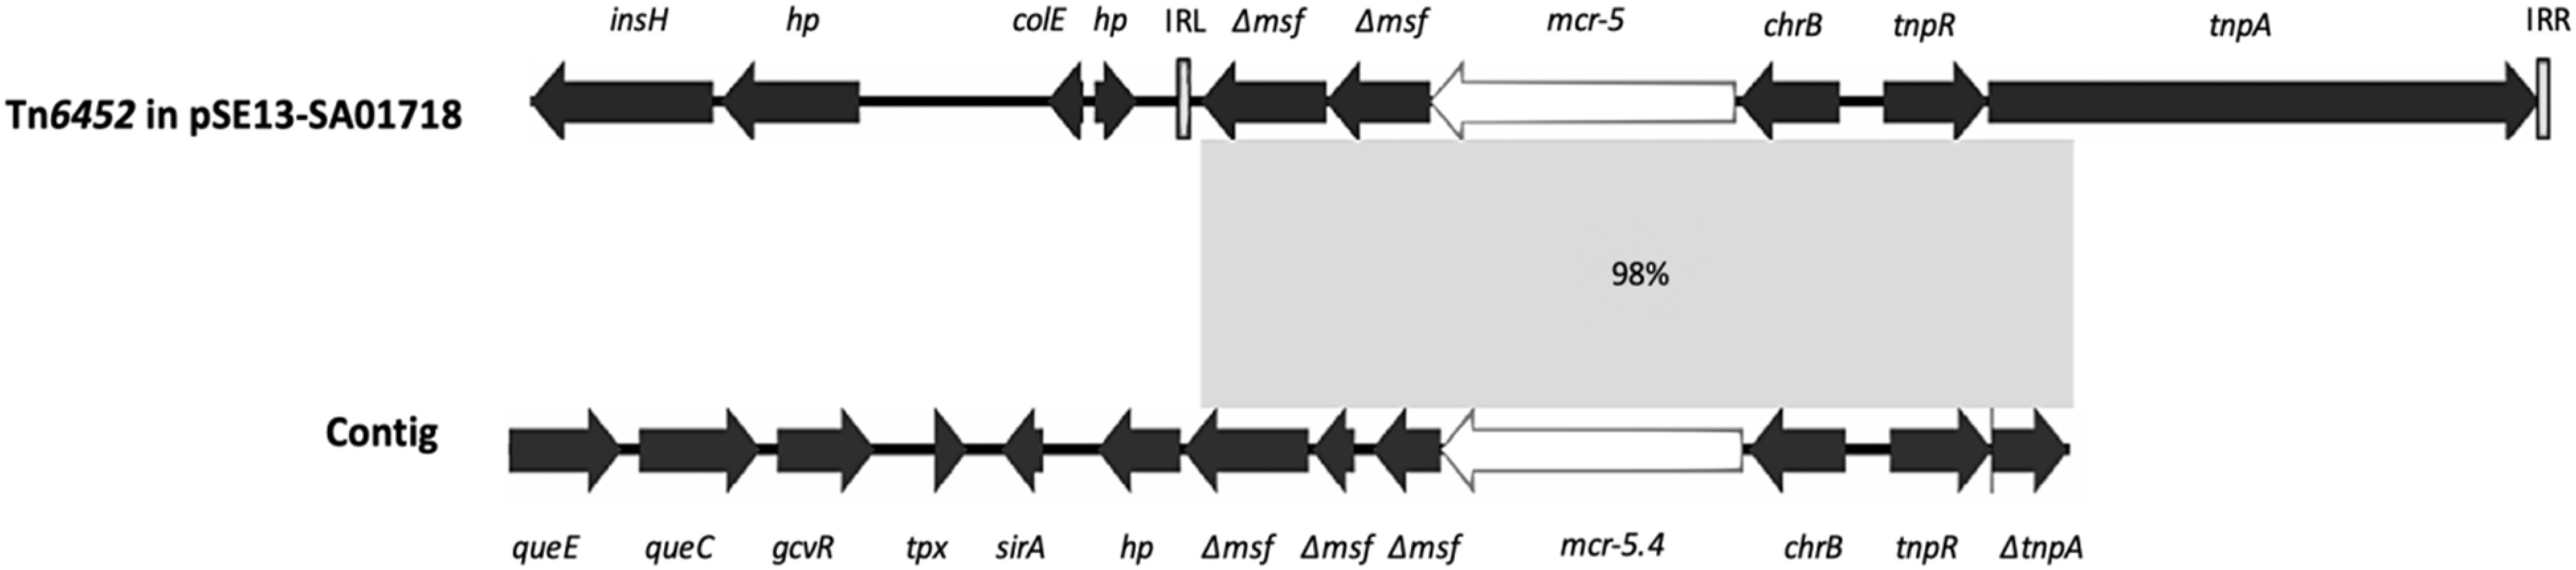
\includegraphics[width=\textwidth]{figures/chapter 3/dkz363f1.jpeg}
\caption{Comparative analysis of the genetic environment of \textit{mcr-5} between the reference plasmid pSE13-SA01718 (accession no. KY807921.1) and the annotated hybrid metagenome contig (accession no. MK965519). The contig carrying the \textit{mcr-5.4} gene consists of the following putative gene products: 7-carboxy-7-deazaguanine synthase (queE), 7-cyano-7-deazaguanine synthase (queC), glycine cleavage system transcriptional antiactivator GcvR (gcvR), thiol peroxidase (tpx), sulphurtransferase TusA family protein (sirA), hypothetical protein (hp), truncated MFS-type transporter ($\Delta$msf), lipid A phosphoethanolamine transferase (\textit{mcr-5.4}), ChrB domain protein (chrB), transposon resolvase (tnpR) and truncated transposon transposase ($\Delta$tnpA). Areas with 98\% identity between sequences are represented in light grey. Arrows indicate the position and direction of the genes. The transposon Tn6452 sequence in the reference plasmid pSE13-SA01718 is bounded by inverted repeats: IRL and IRR.}
\label{fig:chap3_figure1}
\end{figure*}


SRMseq showed the \textit{mcr-5.4} gene detected in a contig of 2113 bp flanked by two truncated protein-coding sequences (CDSs), encoding the ChrB domain protein (involved in chromate resistance) and the Major Facilitator Superfamily (MFS) transporter.
The hybrid-assembly analysis resulted in a contig of 8456 bp consisting of nine CDSs and four truncated CDSs (Figure \ref{fig:chap3_figure1}).
Comparative analysis of the genetic environment of the \textit{mcr-5} gene, between the annotated hybrid metagenome contig and the reference plasmid pSE13-SA01718, showed a region of 4670 bp with 98\% identity, corresponding to the backbone of the Tn6452 transposon (Figure \ref{fig:chap3_figure1}). 
We observed three truncated CDSs for the MFS-type transporter in our contig instead of two as previously described in the reference sequence pSE13-SA01718. 
These differences did not appear to be due to sequencing errors when we checked the sequence MK965519, (i) using pilon (https://github.com/broadinstitute/pilon) to correct for errors in short-read sequencing data and (ii) using CLC Genomic Workbench to update the hybrid contig by mapping both long and short reads against the hybrid contig.
We also observed a region of 3786 bp, with no identity either with the reference plasmid pSE13-SA01718 (Figure \ref{fig:chap3_figure1}) or with any other sequence in the GenBank database.

Species previously described to harbour an \textit{mcr-5} gene are \textit{Escherichia coli}, \textit{Pseudomonas aeruginosa}, \textit{Salmonella enterica}, \textit{Aeromonas hydrophila} and \textit{Cupriavidus gilardii}. 
The bacterial composition analysis of the water sample using SRMseq showed the presence of \textit{Pseudomonas} spp. (relative abundance: 0.004\%), \textit{Cupriavidus} spp. (relative abundance: 0.001\%) and \textit{Aeromonas} spp. (relative abundance: 0.0003\%). 
The binning analysis produced a bin positive for the \textit{mcr-5.4} gene consisting of 1336 contigs (genome size: 5 175 285 bp; genome completeness: 68.2\%). 
This bin was taxonomically classified as bacteria (70.73\%) and proteobacteria (64.90\%), and from this the most abundant class was \textit{Gammaproteobacteria} (37.20\%) (order \textit{Pseudomonadales}, 15.57\%), followed by \textit{Betaproteobacteria} (14.90\%) (order \textit{Burkholderiales}, 10.63\%).

Colistin resistance determinants (\textit{mcr}) have been rarely reported in water environments; \textit{mcr-1} has been detected in both hospital sewage and in environmental water streams and \textit{mcr-3} in environmental water \citep{zhao_incp_2017, tuo_prevalence_2018}.
To the best of our knowledge, this is the first-time description of an \textit{mcr-5} gene in an indoor and healthcare water environment. 
Despite the fact that the comparative analysis showed the hybrid contig covering a large region of Tn6452, neither the left inverted repeat (IRL) nor the right inverted repeat (IRR) have been found. 
In addition, the lack of the right transposon region does not allow us to search for other possible inverted repeats. 
Thus, it is not possible to conclude whether the described \textit{mcr-5.4} gene is transferable or not. 
Taxonomic analysis suggested the order of \textit{Pseudomonadales} as the most probable host of the \textit{mcr-5.4} gene in the water sample. 
Further studies are needed to determine the frequency of this gene in hospital water and other water environments and to evaluate the potential risks for patients and healthcare workers.

\section{Acknowledgements}

We would like to thank Erwin C. Raangs for technical assistance.

\section{Funding}

This project has received funding from the European Union’s Horizon
2020 research and innovation programme under the Marie SklodowskaCurie grant agreement 713660 (MSCA-COFUND-2015-DP ‘Pronkjewail’),
which includes in-kind contributions by commercial partners. None of
the commercial partners had any influence on interpretation of reviewed
data and conclusions drawn, or on drafting of the manuscript. This work
was partly supported by the INTERREG VA (202085)-funded project
EurHealth-1Health, part of a Dutch–German cross-border network supported by the European Commission, the Dutch Ministry of Health,
Welfare and Sport (VWS), the Ministry of Economy, Innovation,
Digitalization and Energy of the German Federal State of North RhineWestphalia and the German Federal State of Lower Saxony.

\section{Transparency declarations}

None to declare.
\newpage
\section{References}
\printbibliography[heading=none]
\end{refsection}

%-----------------------------------------------------------------
% Paper 3 - DEN-IM
%------------------------------------------------------------------
\newpage
\thispagestyle{empty}
\chapter{DEN-IM: Dengue virus genotyping from shotgun and targeted metagenomics\label{ch:paper3}}

\thispagestyle{empty}
\clearpage \thispagestyle{empty}\mbox{}\clearpage
\newpage
\begin{refsection}
\mbox{}\\
\vspace{8cm}

This chapter is a reproduction of the following publication:

C. I. Mendes, E. Lizarazo, M. P. Machado, D. N. Silva, A. Tami, M. Ramirez, N. Couto, J. W. A. Rossen, J. A. Carriço, DEN-IM: dengue virus genotyping from amplicon and shotgun metagenomic sequencing. Microbial Genomics, Volume 6, Issue 3, March 2020. DOI: \url{https://doi.org/10.1099/mgen.0.000328}

The supplementary information referred throughout the text can be consulted in this chapter before the section of references. 

\ac{DENV} represents a public health threat and economic burden in affected countries. The risk of exposure to \ac{DENV} is increasing, not only because of travel to endemic regions, but also due to the broader dissemination of the mosquito vector, making the burden of dengue very significant. 

The availability of genomic data is key to understanding viral evolution and dynamics, supporting improved control strategies. Currently, the use of second-generation sequencing technologies, which can be applied both directly to patient samples (shotgun metagenomics) and to PCR-amplified viral sequences (amplicon sequencing), is the most informative approach to monitor viral dissemination and genetic diversity by providing, in a single methodological step, identification and characterization of the whole viral genome at the nucleotide level. This makes \ac{DENV} identification and characterization through genomic analysis by developing a software where the lessons learned in Chapters \ref{ch:paper1} and \ref{ch:paper2} are applied.

We have developed DEN-IM, a one-stop, user-friendly, containerised and reproducible workflow for the analysis of Dengue virus short-read sequencing data from both amplicon and shotgun metagenomics approaches. EN-IM was designed to perform a comprehensive analysis in order to generate either assemblies or consensus of full DENV coding sequences and to identify their serotype and genotype. DEN-IM can also detect all four DENV serotypes and the respective genotypes present in a spiked sample, raising the possibility that DEN-IM can play a role in the identification of co-infection cases whose prevalence is increasingly perceived in highly endemic areas. 

My contribution to this publication included the design, implementation and optimisation of the DEN-IM the workflow, including the creation of  the Docker containers for all dependencies. Two databases, one comprising 3830 \ac{DENV} sequences for the retrieval of the reads of interest from the input samples, and a second comprising of 161 sequences representing the genetic diversity of all \ac{DENV} sero and genotypes were constructed by me.  Additionally, I've also wrote the manuscript.


\cleardoublepage 

\begin{center}
\large
\textbf{DEN-IM: dengue virus genotyping from amplicon and shotgun metagenomic sequencing}
\end{center}

Catarina I Mendes$^{1,2,*}$, 
Erley Lizarazo$^{2,*}$,
Miguel P Machado$^1$, 
Diogo N Silva$^1$,
Adiana Tami$^2$,
Mário Ramirez$^1$, 
Natacha Couto$^2$, 
John W A Rossen$^2$ and João A Carriço$^1$


$^1$Instituto de Microbiologia, Instituto de Medicina Molecular, Faculdade de Medicina, Universidade de Lisboa, Lisboa, Portugal 

$^2$University of Groningen, University Medical Center Groningen, Department of Medical Microbiology and Infection Prevention, Groningen, The Netherlands

$^*$Contributed equally

\section{Abstract}

Dengue virus (DENV) represents a public health and economic burden in affected countries. The availability of genomic data is key to understanding viral evolution and dynamics, supporting improved control strategies. Currently, the use of High Throughput Sequencing (HTS) technologies, which can be applied both directly to patient samples (shotgun metagenomics) and PCR amplified viral sequences (targeted metagenomics), is the most informative approach to monitor the viral dissemination and genetic diversity.

Despite many advantages, these technologies require bioinformatics expertise and appropriate infrastructure for the analysis and interpretation of the resulting data. In addition, the many software solutions available can hamper reproducibility and comparison of results.
Here we present DEN-IM, a one-stop, user-friendly, containerised and reproducible workflow for the analysis of DENV sequencing data, both from shotgun and targeted metagenomics approaches. It is able to infer the DENV coding sequence (CDS), identify the serotype and genotype, and generate a phylogenetic tree. It can easily be run on any UNIX-like system, from local machines to high-performance computing clusters, performing a comprehensive analysis without the requirement of extensive bioinformatics expertise.

Using DEN-IM, we successfully analysed two DENV datasets. The first comprised 25 shotgun metagenomic sequencing samples of variable serotype and genotype, including an in vitro spiked sample containing the four known serotypes. The second dataset consisted of 106 targeted metagenomic sequences of DENV 3 genotype III where DEN-IM allowed detection of the intra-genotype diversity.
The DEN-IM workflow, parameters and execution configuration files, and documentation are freely available at \url{https://github.com/B-UMMI/DEN-IM}.

\subsection{Keywords}
dengue virus, surveillance, metagenomics, reproducibility, workflow, containerization, scalability
 
\section{Author Notes}
All supporting data, code and protocols have been provided within the article or through supplementary data files.

Metagenomic sequencing data available under BioProject PRJNA474413. DEN-IM reports for the analysed datasets are available in Figshare under https://doi.org/10.6084/m9.figshare.11316599.v1. Phylogeny inference trees for the dengue virus typing database available in Figshare at https://doi.org/10.6084/m9.figshare.11316599.v1. The supplemental material is available in Figshare at https://doi.org/10.6084/m9.figshare.11316599.v1. DEN-IM’s source code and documentation available at https://github.com/B-UMMI/DEN-IM.

%\section{Abbreviations}
 
%\ac{CDS}; 
%Dengue virus ( \ac{DENV}); 
%\ac{HPC}; 
%\ac{HTS}; 
%\ac{NCR}; 
%\ac{QC}; 
%Reverse Transcription Polymerase Chain Reaction (\ac{RT-PCR})

\section{Data Summary}

\begin{enumerate}
    \item The supplemental material and tables are available at Figshare under https://doi.org/10.6084/m9.figshare.9963812
    \item The 106 DENV-3 targeted metagenomics paired-end short-read datasets are available under BioProject PRJNA394021. The 25 shotgun metagenomics dataset is available under BioProject PRJNA474413. The accession number for all the samples in the shotgun metagenomics dataset are available in the Supplementary material
    \item The accession numbers for the 41 samples, belonging to zika virus, chikungunya virus and yellow fever virus shotgun and targeted metagenomic datasets are available in the Supplementary material. 
    \item DEN-IM reports for the analysed datasets are available at Figshare  (https://doi.org/10.6084/m9.figshare.9318851).
    \item Phylogeny inference trees for the dengue virus typing database available at Figshare (https://doi.org/10.6084/m9.figshare.9331826).
    \item Code for the DEN-IM workflow is available at \url{https://github.com/B-UMMI/DEN-IM} and documentation, including step-by-step tutorials, is available at \url{https://github.com/B-UMMI/DEN-IM/wiki}.
\end{enumerate}

\section{Impact Statement}
The risk of exposure to DENV is increasing not only by travelling to endemic regions, but also due to the broader dissemination of the mosquito, making the burden of dengue very significant.

The decreasing costs and wider availability of HTS makes it an ideal technology to monitor DENV’s transmission. Metagenomics approaches decrease the time to obtain nearly complete DENV sequences without the need for time-consuming viral culture through the direct processing and sequencing of patient samples. A ready to use bioinformatics workflow, enabling the reproducible analysis of DENV, is therefore particularly relevant for the development of a straightforward HTS workflow.

DEN-IM was designed to perform a comprehensive analysis in order to generate either assemblies or consensus of full DENV CDSs and to identify their serotype and genotype. DEN-IM can also detect all four DENV genotypes present in a spiked sample, raising the possibility that DEN-IM can play a role in the identification of co-infection cases whose prevalence is increasingly appreciated in highly endemic areas. Although being ready-to-use, the DEN-IM workflow can be easily customised to the user’s needs.

DEN-IM enables reproducible and collaborative research, being accessible to a wide group of researchers regardless of their computational expertise and resources available.

\section{Introduction}

The Dengue virus (DENV), a single-stranded positive-sense RNA virus belonging to the Flavivirus genus, is one of the most prevalent arboviruses and is mainly concentrated in tropical and subtropical regions. Infection with DENV results in symptoms ranging from mild fever to haemorrhagic fever and shock syndrome \citep{organization_dengue_2009}. Transmission to humans occurs through the bite of Aedes mosquitoes, namely Aedes aegypti and Aedes albopictus \citep{diamond_molecular_2015}. In 2010, it was predicted that the burden of dengue disease reached 390 million cases/year worldwide \citep{bhatt_global_2013}. The high morbidity and mortality of dengue makes it the arbovirus with the highest clinical significance \citep{lourenco_challenges_2018}. DENV is a significant public health challenge in countries where the infection is endemic due to the high health and economic burden. Despite the emergence of novel therapies and ecological strategies to control the mosquito vector, there are still important knowledge gaps in the virus biology and its epidemiology \citep{diamond_molecular_2015}.

The viral genome of $\sim$11,000 nucleotides, consists of a CDS of approximately 10.2 Kb that is translated into a single polyprotein encoding three structural proteins (capsid - C, premembrane - prM, envelope - E) and seven non-structural proteins (NS1, NS2A, NS2B, NS3, NS4A, NS4B and NS5). Additionally, the genome contains two Non-Coding Regions (NCRs) at their 5’ and 3’ ends \citep{leitmeyer_dengue_1999}.

DENV can be classified into four serotypes (1, 2, 3 and 4), differing from each other from 25\% to 40\% at the amino acid level. They are further classified into genotypes that vary by up to 3\% at the amino acid level \citep{diamond_molecular_2015}. The DENV-1 serotype comprises five genotypes (I-V), DENV-2 groups six (I-VI, also named American, Cosmopolitan, Asian-American, Asian II, Asian I and Sylvatic), DENV-3 four (I-III and V), and DENV-4 also four (I-IV).

Although real-time reverse transcription polymerase chain reaction (RT-PCR) will probably remain the front line in Dengue etiological diagnosis, the implementation of a surveillance system relying on HTS technologies allows the simultaneous identification and characterization by serotyping and genotyping of DENV cases at the nucleotide level in a single methodological step. Due to the high sensitivity of these technologies, previous studies showed that viral sequences can be directly obtained from patient sera using a shotgun metagenomics approach \citep{yozwiak_virus_2012}. Alternatively, HTS can be used in a targeted metagenomics approach in which a PCR step is used to pre-amplify viral sequences before sequencing. In recent years, HTS has been successfully used as a tool for identification of DENV directly from clinical samples \citep{yozwiak_virus_2012, lee_clinical_2017}. This also allows the rapid identification of the serotype and genotype important for disease management as the genotype may be associated with disease outcome \citep{fatima_serotype_2011}.

Several initiatives aim to facilitate the identification of the DENV serotype and genotype from HTS data. The Genome Detective project (https://www.genomedetective.com/) offers an online Dengue Typing Tool (https://www.genomedetective.com/app/typingtool/dengue/) \citep{fonseca_computational_2019} relying on BLAST and phylogenetic methods in order to identify the closest serotype and genotype, but it requires as input assembled genomes in FASTA format. The same project also offers the Genome Detective Typing Tool (https://www.genomedetective.com/app/typingtool/virus/) \citep{vilsker_genome_2019} identifying viruses present in a sample. Additionally, there are several tools available for viral read identification and assembly, such as VIP \citep{li_vip_2016}, virusTAP \citep{yamashita_virustap_2016} and drVM \citep{lin_drvm_2017}, but none performs genotyping of the identified reads.

We developed DEN-IM as a ready-to-use, one-stop, reproducible bioinformatic analysis workflow for the processing and phylogenetic analysis of DENV using paired-end raw HTS data. DEN-IM is implemented in Nextflow \citep{di_tommaso_nextflow_2017}, a workflow manager software that uses Docker (https://www.docker.com) containers with pre-installed software for all the workflow tools. The DEN-IM workflow, as well as parameters and documentation, are available at \url{https://github.com/B-UMMI/DEN-IM}.

\section{The DEN-IM Workflow}

DEN-IM is a user-friendly automated workflow enabling the analysis of shotgun or targeted metagenomics data for the identification, serotyping, genotyping, and phylogenetic analysis of DENV, as represented in Figure \ref{fig:chap4_figure1}, accepting as input raw paired-end sequencing data (FASTQ files) and informing the user with an interactive and comprehensive HTML report (Supplementary Figure \ref{fig:chap4_figure_sup1}), as well as providing output files of the whole pipeline. 

\begin{figure*}[h!]
\centering
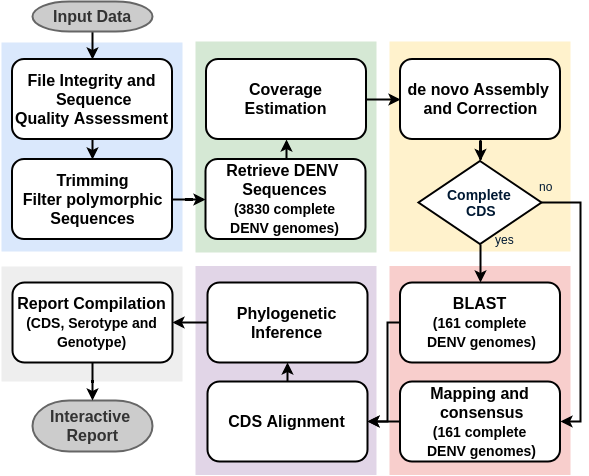
\includegraphics[width=\textwidth]{figures/chapter 4/Figure1_DEN-IM_Diagram.png}
\caption{The DEN-IM workflow separated into five different components. The raw sequencing reads are provided as input to the first block (in blue), responsible for quality control and elimination of low-quality reads and sequences. After successful preprocessing of the reads, these enter the second block (green) for retrieval of the DENV reads using the mapping database of 3858 complete DENV genomes as a reference. This block also provides an initial estimate of the sequencing depth. After the de novo assembly and assembly correction block (yellow), the CDSs are retrieved and then classified with the reduced-complexity DENV typing database containing 161 sequences representing the known diversity of DENV serotypes and genotypes (red). If a complete CDS fails to be assembled, the reads are mapped against the DENV typing database and a consensus sequence is obtained for classification and phylogenetic inference. All CDSs are aligned and compared in a phylogenetic analysis (purple). Lastly, a report is compiled (grey) with the results of all the blocks of the workflow.}
\label{fig:chap4_figure1}
\end{figure*}

It is implemented in Nextflow, a workflow management system that allows the effortless deployment and execution of complex distributed computational workflows in any UNIX-based system, from local machines to \ac{HPC} with a container engine installation, such as Docker (https://www.docker.com/), Shifter \citep{gerhardt_shifter_2017} or Singularity \citep{kurtzer_singularity_2017}. DEN-IM integrates Docker containerised images, compatible with other container engines, for all the tools necessary for its execution, ensuring reproducibility and the tracking of both software code and version, regardless of the operating system used. 

Users can customise the workflow execution either by using command line options or by modifying the simple plain-text configuration files. To make the execution of the workflow as simple as possible, a set of default parameters and directives is provided. An exhaustive description of each parameter is available as Supplementary material (see \ref{chap4_sup_workflow_params}).

The local installation of the DEN-IM workflow, including the docker containers with all the tools needed and the curated DENV database, requires 15 Gigabytes (Gb) of free disk space. The minimum requirements to execute the workflow are at least 5 Gb of memory and 4 CPUs. The disk space required for execution depends greatly on the size of the input data, but for the datasets used in this article, DEN-IM generates approximately 5 Gb of data per Gb input data.
DEN-IM workflow can be divided into the following components:

\subsubsection{Quality Control and Trimming}

The Quality Control (QC) and Trimming block starts with a process to verify the integrity of the input data. If the sequencing files are corrupted, the execution of the analysis of that sample is terminated. The sequences are then processed by FastQC (https://www.bioinformatics.babraham.ac.uk/projects/fastqc/, version 0.11.7) to determine the quality of the individual base pairs of the raw data files. The low-quality bases and adapter sequences are trimmed by Trimmomatic \citep{schmieder_quality_2011} (version 0.36). In addition, paired-end reads with a read length shorter than 55 nucleotides after trimming are removed from further analyses. Lastly, the low complexity sequences, containing over 50\% of poly-A, poly-N or poly-T nucleotides, are filtered out of the raw data using PrinSeq \citep{schmieder_quality_2011} (version 0.10.4).

\subsubsection{Retrieval of DENV sequences}

In the second step, DENV sequences are selected from the sample using Bowtie2 \citep{langmead_fast_2012} (version 2.2.9) and Samtools \citep{langmead_fast_2012} (version 1.4.1). As a reference we provide the DENV mapping database, a curated DENV database composed of 3830 complete DENV genomes. An in-depth description of this database is available as Supplementary material (see \ref{chap4_sup_database}). A permissive approach is followed by allowing for mates to be kept in the sample even when only one read maps to the database in order to keep as many DENV derived reads as possible. The output of this block is a set of processed reads of putative DENV origin.

\subsubsection{Assembly}

DEN-IM applies a two-assembler approach to generate assemblies of the DENV CDS. To obtain a high confidence assembly, the processed reads are first de novo assembled with SPAdes \citep{bankevich_spades_2012} (version 3.12.0). If the full CDS fails to be assembled into a single contig, the data is re-assembled with the MEGAHIT assembler \citep{li_megahit_2015} (version 1.1.3), a more permissive assembler developed to retrieve longer sequences from metagenomics data. The resulting assemblies are corrected with Pilon \citep{walker_pilon_2014} (version 1.22) after mapping the processed reads to the assemblies with Bowtie2.

If more than one complete CDS is present in a sample, each of the sequences will follow the rest of the DEN-IM workflow independently. If no full CDS is assembled neither with SPAdes nor with MEGAHIT, the processed reads are passed on to the next module for consensus generation by mapping, effectively constituting DEN-IM’s two-pronged approach using both assemblers and mapping.

\subsubsection{Typing}

For each DENV complete CDS, the serotype and genotype is determined with the Seq\_Typing tool (\url{https://github.com/B-UMMI/seq\_typing}, version 2.0) \citep{machado_epidemiological_2017} using BLAST \citep{altschul_gapped_1997} and the custom Typing database of DENV containing 161 complete sequences (see \ref{chap4_sup_database}). The tool determines which reference sequence is more closely related to the query based on the identity and length of the sequence covered, returning the serotype and genotype of the reference sequence

If a complete CDS fails to be obtained through the assembly process, the processed reads are mapped against the same DENV typing database, with Bowtie2, using the Seq\_Typing tool, with similar criteria for coverage and identity to those used with the BLAST approach. If a type is determined, the consensus sequence obtained follows through to the next step in the workflow. Otherwise, the sample is classified as Non-Typable and its process terminated.

\subsubsection{Phylogeny}

All DENV complete CDSs and consensus sequences analysed in a workflow execution are aligned with MAFFT \citep{nakamura_parallelization_2018} (version 7.402). By default, or if the number of samples analysed is less than 4, four representative sequences for each DENV serotype (1 to 4) from NCBI are also included in the alignment. The NCBI references included are NC\_001477.1 (DENV-1), NC\_001474.2 (DENV-2), NC\_001475.2 (DENV-3) and NC\_002640.1 (DENV-4). The closest reference sequence to each analysed sample in the DENV typing database to each analysed sample can also be retrieved and included in the alignment. With the resulting alignment, a Maximum Likelihood tree is constructed with RaXML \citep{stamatakis_raxml_2014} (version 8.2.11). 

\subsubsection{Output and Report}

The output files of all tools in DEN-IM’s workflow are stored in the ’results’ folder in the directory of DEN-IM’s execution, as well as the execution log file DEN-IM and for each component. 

The HTML report (Supplementary Figure \ref{fig:chap4_figure_sup1}), stored in the ’pipeline\_results’ directory contains all results divided into four sections: report overview, tables, charts and phylogenetic tree. The report overview and all tables allow for selection, filtering and highlighting of particular samples in the analysis. All tables have information on if a sample failed or passed the quality control metrics highlighted by green, yellow or red signs for pass, warning and fail messages, respectively. 

The \textit{in silico} typing table contains the results of the serotype and genotype of each CDS analysed, as well as identity, coverage and GenBank ID of the closest reference in the DENV typing database. The quality control table shows information regarding the number of raw base pairs and number of reads in the raw input files and the percentage of trimmed reads. The mapping table includes the results for the mapping of the trimmed reads to the DENV mapping database, including the overall alignment rate, and an estimation of the sequence depth including only the DENV reads. For the assembly statistics table, the number of CDSs in each sample, the number of contigs and the number of assembled base pairs generated by either SPAdes or MEGAHIT assemblers is included. The number of contigs and assembled base pairs after correction with Pilon is also presented in the table. The assembled contig size distribution scatter plot is available in the chart section, showing the contig size distribution for the Pilon corrected assembled CDSs.

Lastly, a phylogenetic tree is included, rooted at midpoint for visualisation purposes, and with each tip coloured according to the genotyping results. If the option to retrieve the closest typing reference is selected, these sequences are also included in the tree with respective typing metadata. The tree can be displayed in several conformations provided by Phylocanvas JavaScript library (\url{http://phylocanvas.net}, version 2.8.1) and it is possible to zoom in or collapse selected branches. The support bootstrap values of the branches can be displayed, and the tree can be exported as a Newick tree file or as a PNG image.

\section{Software comparison}

DEN-IM offers a core assembly functionality, leveraging a de novo and consensus assembly approach, to obtain a full CDS sequence to perform geno- and serotyping, followed by phylogenetic positioning of the samples analysed. This results in a phylogenetic tree showing the genotyping results, presented in an HTML file.

There are several alternative tools, both command line and online based, capable of identifying DENV reads and performing assembly (Table \ref{tab:ch4_table1}). VIP and drVM are both stand-alone pipelines, like DEN-IM, and several components overlap with DEN-IM’s but the retrieval of viral sequences is not targeted for DENV, and no serotyping and genotyping is performed. VIP performs a phylogenetic analysis against the reference database. VirusTAP is a web server for the identification of viral reads using the ViPR and IRD databases, or alternatively with the RefSeq Virus database. GenomeDetective is also a web service that provides two tools, one for the assembly of viral sequences from raw data (Virus tool) and another for serotyping and genotyping of DENV fasta sequences (Dengue Typing tool). Both tools need to be run consecutively, with the Virus Tool providing a link to redirect to the Dengue Typing tool when a DENV sequence is identified.

\begin{table}[h!]
\caption{DEN-IM’s workflow comparison with different tools for the identification and genotyping of DENV from sequencing data.}
\label{tab:ch4_table1}
\resizebox{\textwidth}{!}{%
\begin{tabular}{@{}lcccccc@{}}
\toprule
\textbf{Tool} &
  \textbf{Quality Control} &
  \textbf{DENV Sequence Retrieval} &
  \textbf{Assembly} &
  \textbf{Typing} &
  \textbf{Phylogeny} &
  \textbf{Report} \\ \midrule
DEN-IM &
  \checkmark &
  \checkmark &
  \checkmark &
  \checkmark &
  \checkmark &
  \begin{tabular}[c]{@{}c@{}}\checkmark (one report \\ with all samples \\ analysed)\end{tabular} \\
VIP &
  \checkmark &
  \checkmark$^1$ &
  \checkmark &
  X &
  \checkmark &
  \checkmark \\
VirusTAP &
  \checkmark &
  \checkmark$^1$ &
  \checkmark &
  X &
  X &
  \begin{tabular}[c]{@{}c@{}}\checkmark (web-based, \\ one per sample, \\ downloadable)\end{tabular} \\
drVM &
  \checkmark &
  \checkmark$^1$ &
  \checkmark &
  X &
  X &
  X \\
\begin{tabular}[c]{@{}l@{}}GenomeDetective \\ Virus Tool\end{tabular} &
  \checkmark &
  X &
  \checkmark &
  X &
  X &
  \begin{tabular}[c]{@{}c@{}}\checkmark (web-based, \\ one per sample)\end{tabular} \\
\begin{tabular}[c]{@{}l@{}}GenomeDetective \\ Dengue Typing Tool\end{tabular} &
  X &
  X &
  X &
  \checkmark$^2$ &
  X &
  \begin{tabular}[c]{@{}c@{}}\checkmark (web-based, \\ one per sample)\end{tabular} \\ \bottomrule
\end{tabular}%
}
\small
\item $^1$ Targeted for viral sequences, but not specific for DENV
\item $^2$ Sequence file can be received from GenomeDetective Virus Tool, as well as independently uploaded
\end{table}

Of all the tools listed in Table \ref{tab:ch4_table1}, only Genome Detective offers a tool to determine the DENV sero- and genotype from a fasta sequence, but the need to run their virus identification tool prior to obtain a sequence from the raw sequencing data increases the time to obtain a typing result, especially when a large number of sequences needs to be analysed. Moreover, these tools are not open source, so we are unable to compare the methodology used with our own. Additionally, there might be privacy issues in submitting data to external services, like VirusTAP and GenomeDetective, especially when handling metagenomics data that contain human sequences subjected to strict privacy laws in most countries. Therefore, a stand-alone tool is preferable for these analyses since these can be run in secure local environments. DEN-IM’s main advantage when compared to web-based platforms is the ability to analyse batches of samples in a scalable manner, obtaining a report summarizing all the samples analysed and a phylogeny analysis of all DENV CDSs recovered.


\section{Results}

To evaluate the DEN-IM workflow performance, we analysed three datasets, one containing shotgun metagenomics sequencing data of patient samples (see Table \ref{tab:chap4_s1}), a second with amplicon sequencing data, a set with 106 paired-end samples obtained from Parameswaran et al \citep{parameswaran_intrahost_2017} and another set with 78 single-end samples available under BioProject PRJNA321963, and a third dataset of publicly available sequences, both from amplicon and shotgun metagenomics, containing 45 chikungunya virus (CHIKV) samples, 66 zika virus (ZKV), and 21 yellow fever virus (YFV) samples (see Table \ref{tab:chap4_s2}). All analyses were executed with the default resources and parameters (available at \url{https://github.com/B-UMMI/DEN-IM}). In the shotgun metagenomics and the single-end amplicon sequencing datasets the closest typing reference in the final tree and the NCBI DENV references for each serotype were included in the phylogenetic analysis. The resulting reports for each dataset are available on Figshare at \url{https://doi.org/10.6084/m9.figshare.9318851}.

\subsubsection{Shotgun metagenomics dataset}

We analysed a dataset containing 22 shotgun metagenomics paired-end short-read Illumina sequencing samples from positive dengue cases, one positive control (purified from a DENV culture), one negative control (blank), and an in vitro spiked sample containing the 4 DENV serotypes (see \ref{chap4_sup_data}). On average, each sample took 7 minutes to analyse. A total of 75 CPU hours were used to analyse the 25 samples, with a total of 17 Gb in size. This analysis resulted in 69 Gb of data. 
The negative control and the 92-1001 sample had no reads after trimming and filtering of low complexity reads, therefore they were removed from further analysis (see \ref{tab:chap4_s3}). When mapping to the DENV mapping database, the percentage of DENV reads in the 21 clinical samples, positive control and spiked sample passing QC ranged from 0.01\% (sample UCUG0186) to 85.38\% (sample Positive Control - PC). After coverage depth estimation, the analysis of the samples 91-0115 and UCUG0186 was terminated due to a low proportion of DENV reads (0.05\% and 0.01\% respectively). Therefore, they failed to meet the threshold criterion of having an estimated depth of coverage of $\geq$10x (estimated coverages of 3.17x and 5.65x, respectively). Sequence data of sample 91-0106 contained only 960 DENV reads (0.03\%) but these were successfully assembled into a CDS with an estimated depth of coverage of 14.71x.

In the assembly module, the remaining 19 samples, the spiked sample and the PC were assembled with DEN-IM’s two assembler approach. Twenty-four full CDS were assembled (see \ref{fig:chap4_figure_sup2}), even in samples originally having DENV read content as low as 0.03\% of the total reads. Sixteen samples, including the spiked sample and the positive control, were assembled in the first step with the SPAdes assembler, and five in the second with the MEGAHIT assembler. In the spiked sample, all four CDSs were successfully assembled and recovered.

Serotype and genotype were successfully determined for the 24 DENV CDSs by BLAST (see \ref{fig:chap4_figure_sup2}). The most common were serotype 2 genotype III (Asian American) and serotype 4 genotype II, with 8 samples each (33\%), followed by serotype 3 genotype III (n=5, 21\%), serotype 1 genotype V (n=2, 8\%) and serotype 2 genotype V (Asian I) (n=1, 4\%). All CDSs recovered and the respective closest reference genome in the typing database were aligned and a maximum likelihood phylogenetic tree was obtained to visualise the relationship between the samples (Figure \ref{fig:chap4_figure2}). There was a perfect concordance between the results of serotyping and genotyping and the major groups in the tree.
Four distinct CDSs were assembled for the spiked sample that resulted in different coverages of each serotype CDS (2032x times coverage for DENV-2, 229x coverage for DENV-1, 76x coverage for DENV-3 and 30x times coverage for DENV-4), in accordance with the ranking order of the real-time RT-PCR results (see \ref{chap4_sup_data}).

\begin{figure*}[h!]
\centering
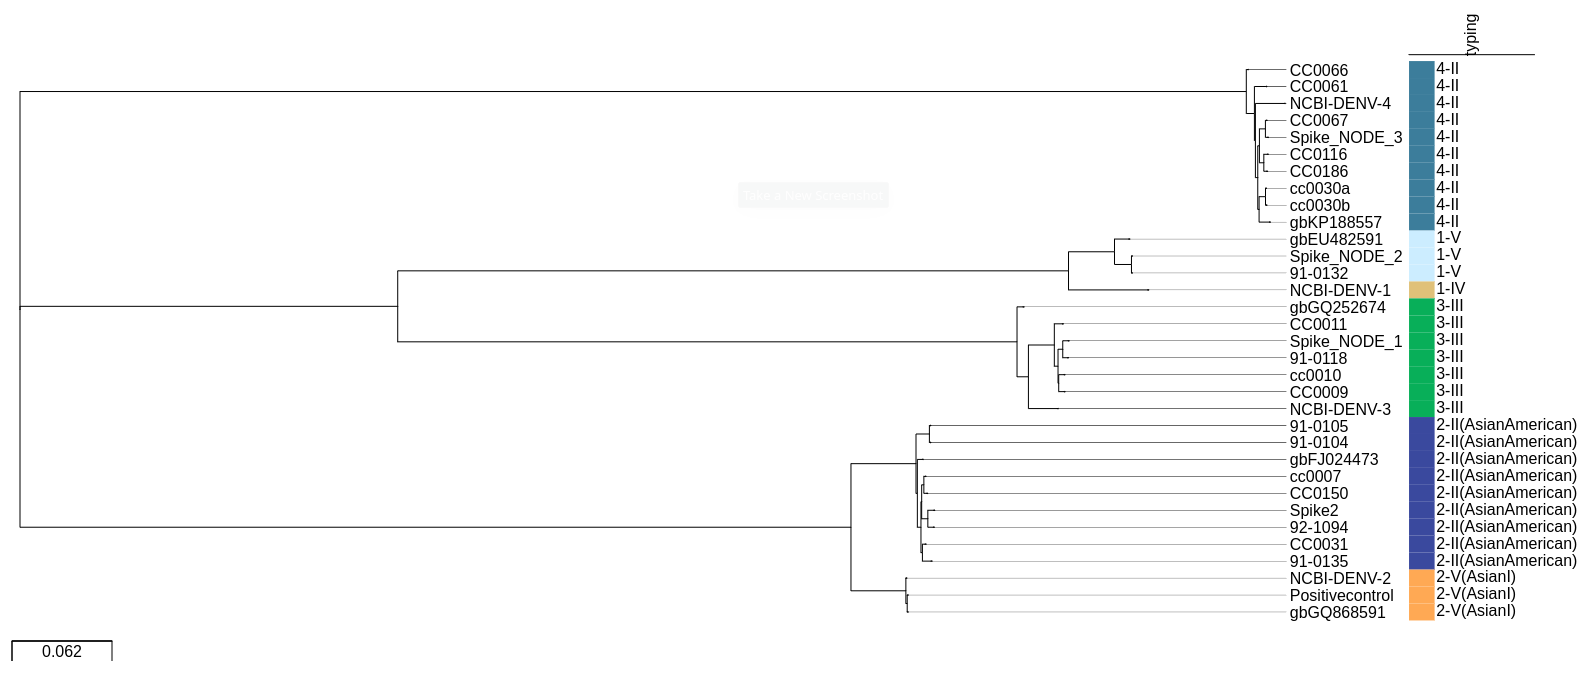
\includegraphics[width=\textwidth]{figures/chapter 4/Figure2_nobranchlabels.png}
\caption{Phylogenetic reconstruction of the shotgun metagenomic dataset. Maximum Likelihood tree in the DEN-IM report for the 24 complete CDSs (n=21 samples) obtained with the metagenomics dataset, the respective closest references in the typing database (identified by their GenBank ID), and the NCBI DENV references for each serotype (NCBI-DENV-1: NC\_001477.1, NCBI-DENV-2: NC\_001474.2, NCBI-DENV-3: NC\_001475.2, NCBI-DENV-4: NC\_002640.1). The tree is midpoint rooted for visualisation purposes and the scale represents average substitutions per site. The colours depict the DENV genotyping results.}
\label{fig:chap4_figure2}
\end{figure*}

\subsubsection{The Amplicon Sequencing Dataset}

To validate DEN-IM’s performance in a amplicon sequencing approach, a dataset of 106 paired-end HTS samples of PCR products using primers targeting DENV-3 (27) were analysed (see \ref{chap4_sup_amplicon}). On average, each sample took 5 minutes to analyse. The 106 samples, with 51 Gb in size, took 3622 CPU hours to be analysed, resulting in 424 Gb of data. 

No samples failed the quality control block (see Table \ref{tab:chap4_s4}). The proportion of DENV reads ranged from 24.72\% (SRR5821236) to 99.81\% (SRR5821254) of the total processed reads. The samples with less than 70\% DENV DNA were taxonomically profiled with Kraken2 (28) and the minikraken2\_v2 database (\url{ftp://ftp.ccb.jhu.edu/pub/data/kraken2_dbs/minikraken2_v2_8GB_201904_UPDATE.tgz}) and the source of contamination was determined to have come largely from Human DNA (see Table \ref{tab:chap4_s5}).

Of the 106 samples, 43 (41\%) managed to assemble a complete CDS sequence (see Table \ref{tab:chap4_s4}) whereas a mapping approach was used for the remaining 63 samples (60\%) and a consensus CDS was generated. For the assembled CDSs, all but one were assembled with MEGAHIT after not producing a full CDS with SPAdes. Moreover, pronounced variation on the size of the assembled contigs is evident in the contig size distribution plot (see \ref{fig:chap4_figure_sup3}).

All 106 CDSs recovered belonged to serotype 3 genotype III. Despite the same classification, the maximum likelihood tree indicates that there is detectable genetic diversity within the dataset (486 SNPs in 10237 nucleotides) (Figure \ref{fig:chap4_figure3}).

\begin{figure*}[h!]
\centering
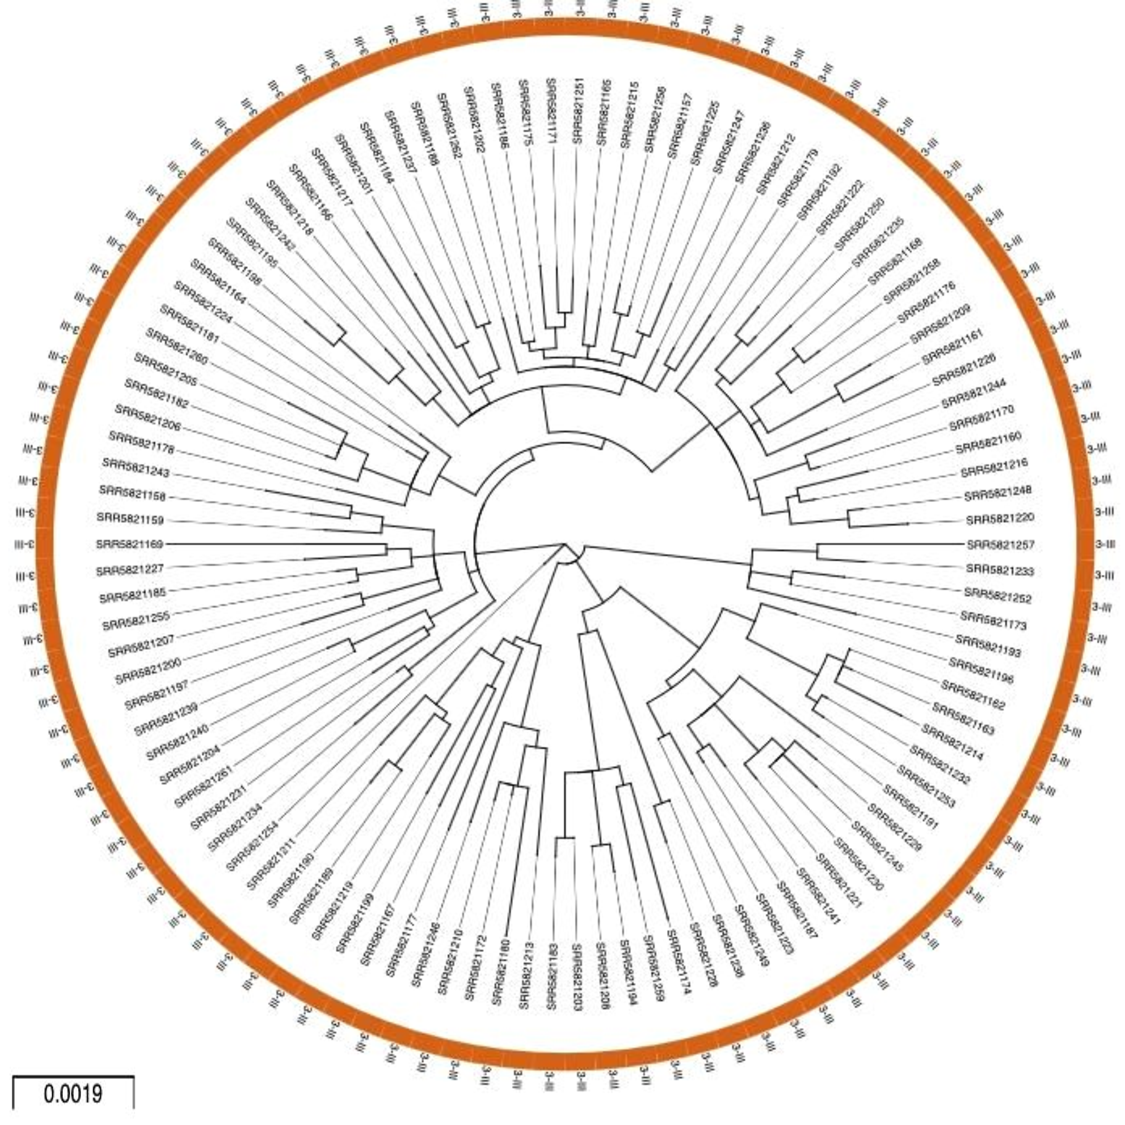
\includegraphics[width=\textwidth]{figures/chapter 4/Figure3_phylo_tree_amplicon.pdf}
\caption{Phylogenetic reconstruction of the paired-end targeted metagenomic dataset. Maximum likelihood circular tree in the DEN-IM report for the 106 complete CDSs obtained with the targeted metagenomics dataset (n=106). All samples belong to serotype 3 genotype III. The scale represents average substitutions per site.}
\label{fig:chap4_figure3}
\end{figure*}

A second amplicon dataset, containing 78 DENV-1 single-end samples recovered from different Aedes aegypti isofemale hosts were analysed (see \ref{chap4_sup_amplicon}). On average, each sample took 3 minutes to analyse. The 78 samples, with 19 Gb in size, took 278 CPU hours to be analysed, resulting in 203 Gb of data.

\begin{figure*}[h!]
\centering
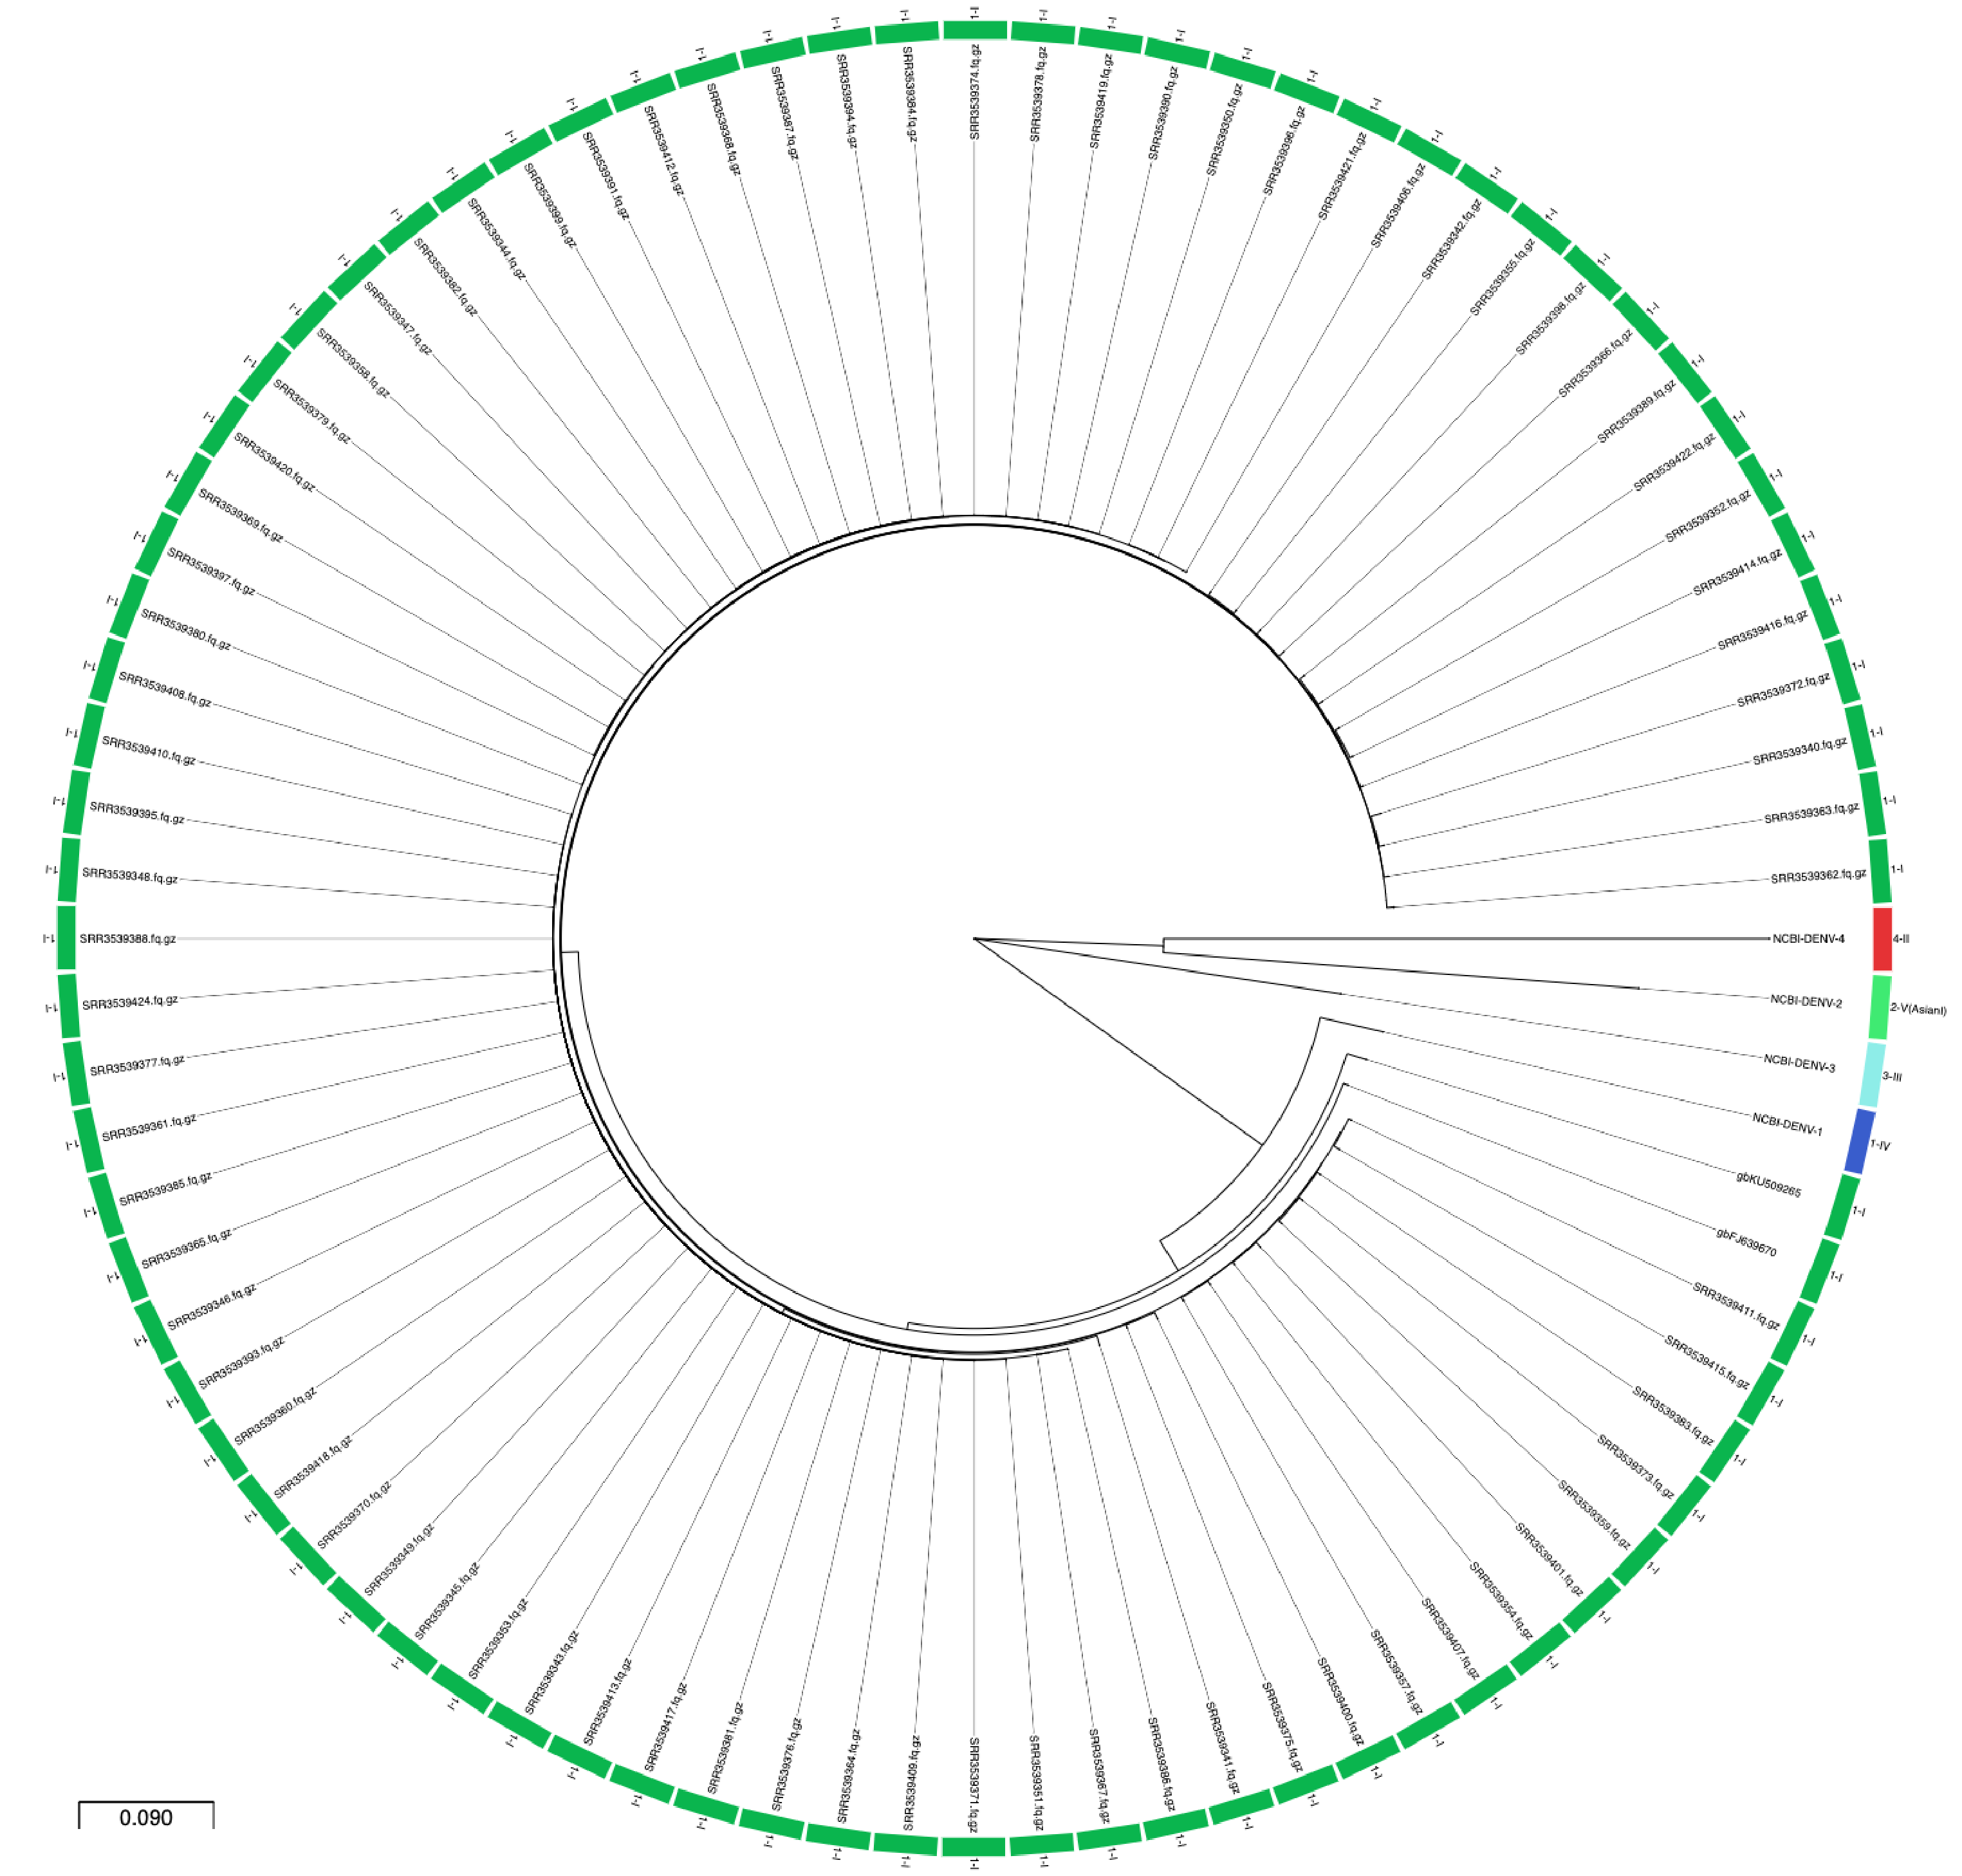
\includegraphics[width=\textwidth]{figures/chapter 4/Figure4.pdf}
\caption{Phylogenetic reconstruction of the single-end targeted metagenomic dataset. Maximum likelihood circular tree in the DEN-IM report for the 78 complete CDSs obtained with the targeted metagenomics dataset (n=78) and the NCBI DENV references for each serotype (NCBI-DENV-1: NC\_001477.1, NCBI-DENV-2: NC\_001474.2, NCBI-DENV-3: NC\_001475.2, NCBI-DENV-4: NC\_002640.1). All samples belong to serotype 1 genotype I. The scale represents average substitutions per site.}
\label{fig:chap4_figure4}
\end{figure*}

No samples failed the quality control block and the proportion of DENV reads ranged from 59\% (SRR3539343) to 96\% (SRR3539408) of the total processed reads (see Table \ref{tab:chap4_s6}). Of the 78 samples, 53 (68\%) assembled a complete CDS sequence and in the remaining 25 (32\%) the complete CDS was obtained through mapping. All CDSs recovered, the respective closest reference genome in the typing database and NCBI’s references for each DENV serotype were aligned and a maximum likelihood phylogenetic tree was obtained (Figure \ref{fig:chap4_figure4}). All 78 samples belong to serotype 1 genotype I and, similarly to the previous dataset of 106 samples, there was detectable genetic diversity within the dataset (651 SNPs in 10808 nucleotides excluding reference sequences).


\subsubsection{The Non-DENV Arbovirus Dataset}

In order to evaluate DEN-IM’s specificity to DENV sequences, a third dataset of publicly available sequences of arbovirus other than DENV, both from amplicon and shotgun metagenomics, was analysed containing 45 CHIKV samples, 66 ZKV, and 21 YFV samples (see Table \ref{tab:chap4_s2}). All 132 samples failed DEN-IM’s workflow, 16 due to not enough sequencing data remaining after quality trimming, and the remaining 116 due to very low estimated coverage of the DENV genome (less than 0.01x), as expected. 

\section{Conclusion}

We have successfully analysed two DENV datasets, one comprising 25 shotgun metagenomics sequencing samples and a second of 106 paired-end and 78 single-end targeted metagenomics samples. 

In the first dataset, we recovered 24 CDSs from 19 clinical samples, including a spiked sample and a positive control that were correctly serotyped and genotyped. Besides the negative control, 3 samples did not return typing information due to failing quality checks.

The proportion of DENV reads in the metagenomics samples was highly variable. This may reflect the viral load in patients in which DENV was detected by real-time RT-PCR. In the spiked sample, containing 4 distinct DENV serotypes, all four were correctly detected despite not being present in equal concentrations, highlighting the potential of the DEN-IM workflow to accurately detect and recover multiple DENV genomes from samples with DENV co-infection, even if the serotypes are present in low abundance. Indeed, recent studies from areas of high endemicity suggest that co-infection with multiple DENV serotypes may frequently occur \citep{marinho_meningitis_nodate, reddy_occurrence_2017} and the co-circulation of different DENV strains of the same serotype, but distinct genotypes, in these areas \citep{marinho_meningitis_nodate} raises the possibility of simultaneous infection with more than one genotype.

When analysing the 106 paired-end targeted metagenomics dataset, only 43 CDS samples were de novo assembled. For the remaining 63 samples, consensus sequences were obtained through mapping. In all samples DENV 3-III was correctly identified. Similar results were obtained for the 78 single-end samples where 53 CDS were de novo assembled, and 25 consensus sequences were obtained through mapping. All samples were identified as DENV-1 I. These two datasets demonstrate the success of DEN-IM’s two-pronged approach of combining assembler and mapping. DEN-IM’s specificity was shown when it found no false positive results when analysing a dataset containing arboviruses other than DENV. 

DEN-IM is built with modularity and containerisation as keystones, leveraging the parallelization of processes and guaranteeing reproducible analyses across platforms. The modular design allows for new modules to be easily added and tools that become outdated to be easily updated, ensuring DEN-IM’s sustainability. The software versions are also described in the Nextflow script and configuration files, and in the dockerfiles for each container, allowing the traceability of each step of data processing.

Being developed in Nextflow, DEN-IM runs on any UNIX-like system and provides out-of-the-box support for several job schedulers (e.g., PBS, SGE, SLURM) and integration with containerised software like Docker or Singularity. While it has been developed to be ready to use by non-experts, not requiring any software installation or parameter tuning, it can still be easily customised through the configuration files.

The interactive HTML reports (see \ref{fig:chap4_figure_sup1}) provide an intuitive platform for data exploration, allowing the user to highlight specific samples, filter and re-order the data tables, and export the plots as needed.

Together with the workflow and software containers, a database containing 3858 complete DENV genomes for DENV sequence retrieval and a subset database with 161 curated DENV genomes for serotyping and genotyping are provided. While constructing these databases, the obstacles reported by Cuypers et al \citep{cuypers_time_2018} were apparent, namely the lack of formal definition of a DENV genotype and the lack of a standardised classification procedure that could assign sequences to a previously defined genotypic/sub-genotypic clade \citep{cuypers_time_2018}. Discrepancies between the phylogenetic relationship and the genotype assignment were frequent and, throughout this study, the classification of some strains within the ViPR database \citep{pickett_virus_2012} was updated. As suggested previously \citep{cuypers_time_2018}, further evaluation of the DENV classification will benefit future research and investigation into the population dynamics of this virus. Our typing approach was designed to use the currently accepted DENV classification. However, DEN-IM can be easily modified if a new DENV classification system is to be established in the future.

DEN-IM provides a user-friendly workflow that makes it possible to analyse short-read raw sequencing data from shotgun or targeted metagenomics for the presence, typing and phylogenetic analysis of DENV. The use of containerised workflows, together with shareable reports, will allow an easier comparison of results globally, promoting collaborations that can benefit the populations where DENV is endemic. The DEN-IM source code is freely available in the DEN-IM GitHub repository (\url{https://github.com/B-UMMI/DEN-IM}), which includes a wiki with full documentation and easy to follow instructions.

\section{Author Statements}

\subsection{Authors and contributions}

C.I.M., E.L., N.C., M.R., J.A.C. and J.W.A.R. designed the workflow. C.I.M implemented and optimised the workflow, created the Docker containers, and wrote the manuscript. M.P.M. implemented the DENV genotyping module in the workflow and D.N.S. contributed to the development of DEN-IM’s HTML report. E.L., A. T., and N.C. provided the shotgun metagenomics data used to test and validate the workflow and wrote the manuscript. A.T., N.C., M.R., J.A.C. and J.W.A.R. critically revised the article. All authors read, commented on, and approved the final manuscript.

\subsection{Conflict of interest}

The authors declare that they have no competing interests.

\subsection{Funding information}

C.I.M. was supported by the Fundação para a Ciência e Tecnologia (grant SFRH/BD/129483/2017). Erley Lizarazo received the Abel Tasman Talent Program grant from the UMCG, University of Groningen, Groningen, The Netherlands. This work was partly supported by the ONEIDA project (LISBOA-01-0145-FEDER-016417) co-funded by FEEI–Fundos Europeus Estruturais e de Investimento from Programa Operacional Regional Lisboa 2020 and by national funds from FCT–Fundação para a Ciência e a Tecnologia and by UID/BIM/50005/2019, project funded by Fundação para a Ciência e a Tecnologia (FCT)/ Ministério da Ciência, Tecnologia e Ensino Superior (MCTES) through Fundos do Orçamento de Estado.

\subsection{Ethical approval}

This study followed international standards for the ethical conduct of research involving human subjects. Data and sample collection was carried out within the DENVEN and IDAMS (International Research Consortium on Dengue Risk Assessment, Management and Surveillance) projects. The study was approved by the Ethics Review Committee of the Biomedical Research Institute, Carabobo University (Aval Bioetico \#CBIIB(UC)-014 and CBIIB-(UC)-2013-1), Maracay, Venezuela; the Ethics, Bioethics and Biodiversity Committee (CEBioBio) of the National Foundation for Science, Technology and Innovation (FONACIT) of the Ministry of Science, Technology and Innovation, Caracas, Venezuela; the regional Health authorities of Aragua state (CORPOSALUD Aragua) and Carabobo State (INSALUD); and by the Ethics Committee of the Medical Faculty of Heidelberg University and the Oxford University Tropical Research Ethics Committee.

\subsection{Consent for publication}

All individuals, or a parent or legal guardian if under 16 years of age, whose sample and data were collected have given consent to participate in the study.

\subsection{Acknowledgements}

The authors would like to thank Tiago F. Jesus and Bruno Ribeiro-Gonçalves for their invaluable help with the Nextflow implementation. We would also like to thank Erwin C. Raangs from the UMCG for his assistance in the sequencing of the shotgun metagenomics dataset. Additionally, the authors thank Lize Cuypers, Krystof Theys, Pieter Libin and Gilberto Santiago for their discussions on DENV nomenclature and classification. This work was done in collaboration with the ESCMID Study Group on Molecular and Genomic Diagnostics (ESGMD), Basel, Switzerland.

\section{Data Bibliography}
\begin{itemize}
    \item Catarina Inês Mendes. DEN-IM supplemental material and tables are deposited at Figshare with DOI 10.6084/m9.figshare.9963812 (https://doi.org/10.6084/m9.figshare.9963812.v3).
    \item Catarina Inês Mendes. DEN-IM reports for the analysed datasets tables are deposited at Figshare with DOI 0.6084/m9.figshare.9318851 (https://doi.org/10.6084/m9.figshare.9318851).
    \item Catarina Inês Mendes. Phylogeny inference trees for the dengue virus typing database are deposited at Figshare with DOI 10.6084/m9.figshare.9331826 (https://doi.org/10.6084/m9.figshare.9331826).
    \item Catarina Inês Mendes. Code for the DEN-IM workflow (https://github.com/B-UMMI/DEN-IM).
\end{itemize}

\section{Supplementary Material}

\subsection{Dengue virus reference databases} \label{chap4_sup_database}

We have compiled a database of 3858 complete DENV genomes obtained from the NIAID Virus Pathogen Database and Analysis Resource (ViPR) in October 2019 \citep{pickett_virus_2012} (\url{http://www.viprbrc.org/}).The sequences were distributed unevenly throughout the four DENV serotypes, with DENV-1 being the most represented with 1636 sequences (42.72\%), followed by DENV-2 with 1067 sequences (27.86\%), DENV-3 with 807 sequences (21.07\%), and DENV-4 with 320 sequences (8.36\%). The selection criteria for the search were as follows: a) complete genome sequence only, b) human or mosquito host, c) collection year (1950-2018). Data available from all countries was included and duplicated sequences were removed and only the sequences with sub-type data were kept. A representative of DENV serotype 1 genotype III was introduced (EF457905, recovered from monkey) as no representatives were available with the search criteria used. This genotype is sylvatic and considered extinct \citep{villabona-arenas_worldwide_2013, vasilakis_history_2008}. Additionally, any sample with IUPAC codes in the sequence provided were excluded. 

In order to recover the maximum number of DENV reads from the input HTS data in the first mapping step (Figure \ref{fig:chap2_figure1}), we maintained the database with the 3858 complete DENV genomes to retain as much diversity as possible. This database is referred as DENV mapping database and is available on GitHub at \url{https://github.com/B-UMMI/DEN-IM/blob/master/ref/DENV_MAPPING_V3.fasta}. 

For typing purposes, overly similar sequences in the collection were removed from the database by clustering the sequences in each serotype at 98\% nucleotide similarity with CD-HIT \citep{li_cd-hit_2006}, leaving 161 representative sequences of all described DENV serotypes and genotypes, with 46 DENV-1 sequences (Table \ref{tab:chap4_s7}), 63 DENV-2 (Table \ref{tab:chap4_s8}), 25 DENV-3 (Tables \ref{tab:chap4_s9}) and 27 DENV-4 (Table \ref{tab:chap4_s10}). This database is referred as DENV typing database and is available on GitHub at \url{https://github.com/B-UMMI/DEN-IM/blob/master/ref/DENV_TYPING_V3.fasta}. This step is necessary to speed up the classification step for genotyping.

Phylogenetic analysis of typing collection was performed by aligning the full reference genomes with MAFFT \citep{nakamura_parallelization_2018}, in auto mode and with automatic sequence orientation adjustment. A phylogenetic tree was inferred with RAxML (version 8.12.11) \citep{stamatakis_raxml_2014} using the GTR-$\Gamma$ substitution model and 500 times bootstrap. Additionally, the same analysis was performed with the envelope protein (E) only, as this region has been used traditionally for sero- and genotyping \citep{rico-hesse_molecular_1990, rico-hesse_microevolution_2003, lanciotti_rapid_1992, lanciotti_molecular_1997, klungthong_molecular_2004, zhang_clade_2005, zhang_structure_2006}, and continues to be the standard in many laboratories for genotyping. The resulting trees are available as supplemental material (Figures \ref{fig:chap4_figure_sup4} to \ref{fig:chap4_figure_sup7}) and on Figshare (\url{https://10.6084/m9.figshare.9331826}).

The sequence JF459993 from the DENV-1 collection, as of April 2019, was annotated in ViPR as belonging to genotype IV, but in our analysis, it clustered within genotype I clade (Figure \ref{fig:chap4_figure_sup4}). The classification of DENV-1 I was also obtained from GenomeDetective Dengue Subtyping Tool (\url{https://www.genomedetective.com/app/typingtool/dengue/}), so we proceeded to alter the annotation of this particular sample (Table \ref{tab:chap4_s6}). 
In order to harmonise dengue nomenclature, the system uses Roman-numeric labels to identify the genotype, with the exception of Serotype 2 (Table \ref{tab:chap4_s4}), which used both Roman-numeric and geographic origin due to the widespread adoption of the latter.

\subsection{Workflow parameters} \label{chap4_sup_workflow_params}

The short-read data is passed as input through the “--fastq” parameter, that by default is set to match all files in the “fastq” folder that match the pattern “*\_R{1,2}*”. Both paired and single-end sequencing data can be passed through with the “--fastq” parameter, as defined by the pattern used. 

In the process to verify the integrity of the short-read raw sequencing data, the integrity of the input files is assessed by attempting to decompress and read the files. An estimation of the depth of coverage is also performed. By default, the input size ("–-genomeSize") is set to 0.012 Mb and the minimum coverage depth ("–-minCoverage") is set to 10. If any input file is found to be corrupt, its progression in the workflow is aborted.

In the FastQC and Trimmomatic module, FastQC (https://www.bioinformatics.babraham.ac.uk/projects/fastqc/) is run with the parameters "–extract –nogroup –format fastq". FastQC will inform Trimmomatic \citep{bolger_trimmomatic_2014} on how many bases to trim from the 3’and 5’ ends of the raw reads. By default, Trimmomatic uses the default set of Illumina adapters provided with the workflow but this behaviour can be overwritten with the "–-adapters" parameter. The additional Trimmomatic parameters "-–trimSlidingWindow", "–-trimLeading", "–-trimTrailing" and "–-trimMinLength"can all be set to different values.

The removal of low complexity sequences is done with PrinSeq \citep{schmieder_quality_2011} using a custom parameter ("–pattern"), which by default is set to the value "A 50\%; T 50\%; N 50\%", removing sequences whose content is at least half composed of a polymeric sequence (A, T or N).

To retrieve the reads that map to the DENV reference database, Bowtie2 \citep{langmead_fast_2012} is run with default parameters with the DENV mapping database as a reference. For paired-end data, the reads and their mates that map to the reference are retrieved with "samtools view -buh -F 12" and "samtools fastq" commands. In single-end reads, all mapped reads are retrieved with "samtools view -buh -F 4" and "samtools fastq". The DENV mapping database can be altered with the "–-reference" parameter, or alternatively, a Bowtie2 index can be provided with the "–-index" parameter. This allows for the workflow to work with other databases obtained through public and owned DENV genomes. The coverage estimation step is performed on the retrieved DENV reads with the same parameters are the first estimation ("–-genomeSize=0.012" and "–-minCoverage=10").

In the assembly process, the retrieved DENV reads are firstly assembled with SPAdes Genome Assembler \citep{bankevich_spades_2012} with the options "–careful –only-assembler –cov-cutoff". The coverage cut-off if dictated by the "–-spadesMinCoverage" and "–-spadesMinKmerCoverage" parameters, set to 2 by default. If the assembly with SPAdes fails to produce a contig equal or greater than the value defined in the "–minimumContigSize" parameter (default of 10000), the data is re-assembled with the MEGAHIT assembler \citep{li_megahit_2015} with default parameters. By default, the k-mers to be used in the assembly in both tools ("–spadesKmers" and "–megahitKmers") are automatically determined depending on the read size. If the maximum read length is equal or greater than 175 nucleotides, the assembly is done with the k-mers "55, 77, 99, 113, 127", otherwise the k-mers "21, 33, 55, 67, 77" are used.

To correct the assemblies produced, the Pilon tool \citep{walker_pilon_2014} is run after mapping the QC’ed reads back to the assembly with Bowtie2 and "samtools sort". This process also verifies the coverage and the number of contigs produced in the assembly. The behaviour can be altered with the parameters "–minAssemblyCoverage", "–AMaxContigs" and "–genomeSize", set to "auto", 1000 and 0.01 Mb by default. The first parameter, when set to ’auto’, the minimum assembly coverage for each contig required is set to the 1/3 of the assembly mean coverage or to a minimum of 10x. The ratio of contig number per genome MB is calculated based on the genome size estimation for the samples.
The contigs larger than the value defined in the "–size" parameter (default of 10000 nucleotides) are considered to be complete CDSs and follow the rest to the workflow independently. If no complete CDS is recovered, the QC’ed read data is passed to the mapping to module that does the DENV typing database and consensus generation. 

The serotyping and genotyping are performed with the Seq\_Typing tool \citep{machado_epidemiological_2017} with the command "seq\_typing.py assembly" or "seq\_typing.py reads", using as reference the provided curated DENV typing database. It is possible to retrieve the genomes of the closest references and include them in the downstream analysis by changing the "–get\_reference" option to "true". By default, this is not included in the analysis.

The CDSs, and the reference sequences if requested, are aligned with the MAFFT tool \citep{nakamura_parallelization_2018} with the options "–adjustdirection –auto". By default, four representative sequences for each DENV serotype (1 to 4) from NCBI is also included in the alignment. This option can be turned off by changing the value of “--includeNCBI” to "false". If the number of sequences in the alignment is less than 4 these are automatically added. 

A maximum likelihood phylogenetic tree is obtained with the RaXML tool \citep{stamatakis_raxml_2014} with the options "-p 12345 -f -a". Additionally, and by default, the substitution model ("–substitutionModel") is set to "GTRGAMMA", the bootstrap is set to 500 ("–bootstrap") and the seed to "12345" ("–seedNumber").

\subsection{Shotgun Metagenomics Sequencing Data} \label{chap4_sup_data}

Samples of plasma (n=9) and serum samples (n=13) from confirmed dengue symptomatic patients were collected in Venezuela between 2010-2015 (Table S2) (see Availability of supporting materials). DENV positivity was confirmed by either RT-qPCR \citep{santiago_analytical_2013} or nested RT-PCR \citep{lanciotti_rapid_1992}. 

As a positive control sample, the supernatant of a viral culture containing DENV-2 strain 16681 was used. The negative control sample consisted of DNA- and RNA-free water (Sigma-Aldrich, St. Louis, MO, USA). 

A spiked sample was produced consisting of a mixture of four 5 µl of cDNA isolated from clinical samples including all DENV serotypes (DENV-1 to -4). The viral cDNA for these samples was not in equal concentration and the viral copy number in the clinical samples was assessed by RT-PCR \citep{lanciotti_rapid_1992}. The results were as follow: DENV-2 with 1070000 copies/µl, DENV-1 with 117830 copies/µl, DENV-3 with 44300 copies/µl and DENV-4 with 6600 copies/µl.

The cDNA libraries were generated using either the NEBNext® RNA First and Second strand modules and the Nextera XT DNA library preparation kit (NXT), or the TruSeq RNA V2 library preparation kit (TS). The libraries were sequenced in MiSeq and NextSeq instruments using 300-cycles v2 paired-end cartridges.

The DEN-IM workflow was executed with the raw sequencing data using the default parameters and resources in an HPC cluster with 300 Cores/600 Threads of Processing Power and 3 TB RAM divided through 15 computational nodes, 9 with 254 GB Ram and 6 with 126GB RAM.

\subsection{Amplicon Sequencing Data} \label{chap4_sup_amplicon}

The accession numbers for the 106 DENV-3 paired-end amplicon sequencing paired-end short-read datasets are available under BioProject PRJNA394021. The accession numbers for the 78 DENV-1 amplicon sequencing single-end short-read datasets are available under BioProject PRJNA321963. The Run Accession IDs for both sets were obtained with NCBI’s RunSelector and the raw data was downloaded with the GetSeqENA tool (https://github.com/B-UMMI/getSeqENA).

The DEN-IM workflow was executed with the raw sequencing data with default parameters and resources in the same HPC cluster as the shotgun metagenomics dataset.

\subsection{Non-DENV Arbovirus Data} \label{chap4_sup_non_denv}

The accession numbers for the 132 samples, belonging to zika virus (ZKV), chikungunya virus (CHIKV) and yellow fever virus (YFV) amplicon and metagenomic datasets are available as supplemental material (Table S4). As with the amplicon sequencing dataset, the list of Run Accession IDs was obtained with NCBI’s RunSelector and the raw data was downloaded with the GetSeqENA tool (\url{https://github.com/B-UMMI/getSeqENA}). 

The DEN-IM workflow was executed with default parameters and resources in the same HPC cluster as the amplicon and shotgun metagenomics datasets.

\subsection{Supplemental Tables} \label{chap4_sup_tables}

\begin{table}[h!]
\caption{Collection date, serotype confirmation and run accession identifier for the metagenomic sequencing dataset.}
\label{tab:chap4_s1}
\resizebox{\textwidth}{!}{%
\begin{tabular}{@{}lllllll@{}}
\toprule
\textbf{Sample} & \textbf{Collection   Date} & \textbf{Source} & \textbf{Serotype   (qPCR)} & \textbf{Serotype} & \textbf{Genotype}            & \textbf{Run Accession} \\ \midrule
91-0104          & 21/9/2015  & plasma & 2 & 2 & III(AsianAmerican) & SRR8842525 \\
91-0105          & 22/9/2015  & plasma & 2 & 2 & III(AsianAmerican) & SRR7252349 \\
91-0115          & 30/9/2015  & plasma & 3 & - & -                  & SRR7252368 \\
91-0118          & 5/10/2015  & plasma & 3 & 3 & III                & SRR7252362 \\
91-0132          & 19/10/2015 & plasma & 1 & 1 & V                  & SRR8883926 \\
91-0135          & 27/10/2015 & plasma & 2 & 2 & III(AsianAmerican) & SRR9004764 \\
92-1001          & 2/10/2015  & plasma & 1 & - & -                  & SRR7252337 \\
92-1094          & 16/10/2015 & plasma & 2 & 2 & III(AsianAmerican) & SRR8842524 \\
CC0007           & 31/8/2010  & serum  & 2 & 2 & III(AsianAmerican) & SRR7252354 \\
CC0009           & 31/8/2010  & serum  & 3 & 3 & III                & SRR8842527 \\
CC0010           & 27/8/2010  & serum  & 3 & 3 & III                & SRR7252358 \\
CC0011           & 27/8/2010  & serum  & 3 & 3 & III                & SRR8842526 \\
CC0030a          & 1/9/2010   & serum  & 4 & 4 & II                 & SRR7252356 \\
CC0030b          & 1/9/2010   & serum  & 4 & 4 & II                 & SRR7252355 \\
CC0031           & 2/9/2010   & serum  & 2 & 2 & III(AsianAmerican) & SRR8842521 \\
CC0061           & 20/1/2011  & serum  & 4 & 4 & II                 & SRR8842520 \\
CC0066           & 11/10/2011 & serum  & 4 & 4 & II                 & SRR8842523 \\
CC0067           & 18/10/2011 & serum  & 4 & 4 & II                 & SRR8842522 \\
CC0116           & 29/3/2012  & serum  & 4 & 4 & II                 & SRR8842519 \\
CC0150           & 9/5/2012   & serum  & 2 & 2 & III(AsianAmerican) & SRR8842518 \\
CC0186           & 17/7/2012  & serum  & 4 & 4 & II                 & SRR9004763 \\
UCUG0186         & 30/8/2010  & serum  & 4 & 4 & II                 & SRR8842528 \\
Negative Control & -          & -      & - & - & -                  & SRR8842530 \\
Positive Control & -          & -      & 2 & 2 & V(AsianI)          & SRR8886136 \\
Spiked   sample & -                          & -               & 1,2,3,4                    & 1,2,3,4           & V,III(Asian American),III,II & SRR8842529             \\ \bottomrule
\end{tabular}%
}
\end{table}

\newpage

\begin{scriptsize}
\begin{center}

\begin{longtable}{@{}lllll@{}}
\caption{Run accession ID, BioProject SRA Study ID, source and organism present for each sample of the negative control dataset (ZKV – zika virus, CHIKV – chikungunya virus, YFV – yellow fever virus).}
\label{tab:chap4_s2}\\

\toprule
Run ID     & Bioproject  & SRA Study & Source                & Organism \\ \midrule
\endfirsthead

\multicolumn{5}{l}{\tablename \thetable - \textit{Continued from previous page} }\\
\toprule
Run ID     & Bioproject  & SRA Study & Source                & Organism \\ \midrule
\endhead

\bottomrule
\multicolumn{5}{r}{\textit{Continue on next page}}\\
\endfoot

\bottomrule
\endlastfoot

SRR8031152 & PRJNA494391 & SRP163225 & Shotgun Metagenomic   & ZKV      \\
SRR8062732 & PRJNA494391 & SRP163225 & Shotgun Metagenomic   & ZKV      \\
SRR8031153 & PRJNA494391 & SRP163225 & Shotgun Metagenomic   & ZKV      \\
SRR8063606 & PRJNA494391 & SRP163225 & Shotgun Metagenomic   & ZKV      \\
SRR8063603 & PRJNA494391 & SRP163225 & Shotgun Metagenomic   & ZKV      \\
SRR8063605 & PRJNA494391 & SRP163225 & Shotgun Metagenomic   & ZKV      \\
SRR8031155 & PRJNA494391 & SRP163225 & Shotgun Metagenomic   & ZKV      \\
SRR8031154 & PRJNA494391 & SRP163225 & Shotgun Metagenomic   & ZKV      \\
SRR8063604 & PRJNA494391 & SRP163225 & Shotgun Metagenomic   & ZKV      \\
SRR8062733 & PRJNA494391 & SRP163225 & Shotgun Metagenomic   & ZKV      \\
SRR7985391 & PRJNA494391 & SRP163225 & Shotgun Metagenomic   & ZKV      \\
SRR7985394 & PRJNA494391 & SRP163225 & Shotgun Metagenomic   & ZKV      \\
SRR7985620 & PRJNA494391 & SRP163225 & Shotgun Metagenomic   & CHIKV    \\
SRR7985390 & PRJNA494391 & SRP163225 & Shotgun Metagenomic   & ZKV      \\
SRR7985392 & PRJNA494391 & SRP163225 & Shotgun Metagenomic   & ZKV      \\
SRR7985621 & PRJNA494391 & SRP163225 & Shotgun Metagenomic   & CHIKV    \\
SRR5179639 & PRJNA361543 & SRP096859 & Amplicon Metagenomics & YFV      \\
SRR5179637 & PRJNA361543 & SRP096859 & Amplicon Metagenomics & YFV      \\
SRR5179646 & PRJNA361543 & SRP096859 & Amplicon Metagenomics & YFV      \\
SRR7985389 & PRJNA494391 & SRP163225 & Shotgun Metagenomic   & ZKV      \\
SRR7985622 & PRJNA494391 & SRP163225 & Shotgun Metagenomic   & CHIKV    \\
SRR7985619 & PRJNA494391 & SRP163225 & Shotgun Metagenomic   & CHIKV    \\
SRR5179667 & PRJNA361543 & SRP096859 & Amplicon Metagenomics & YFV      \\
SRR5179653 & PRJNA361543 & SRP096859 & Amplicon Metagenomics & YFV      \\
SRR7985393 & PRJNA494391 & SRP163225 & Shotgun Metagenomic   & ZKV      \\
SRR5179638 & PRJNA361543 & SRP096859 & Amplicon Metagenomics & YFV      \\
SRR5179636 & PRJNA361543 & SRP096859 & Amplicon Metagenomics & YFV      \\
SRR5179666 & PRJNA361543 & SRP096859 & Amplicon Metagenomics & YFV      \\
SRR5179650 & PRJNA361543 & SRP096859 & Amplicon Metagenomics & YFV      \\
SRR5179649 & PRJNA361543 & SRP096859 & Amplicon Metagenomics & YFV      \\
SRR5179643 & PRJNA361543 & SRP096859 & Amplicon Metagenomics & YFV      \\
SRR5179635 & PRJNA361543 & SRP096859 & Amplicon Metagenomics & YFV      \\
SRR5179645 & PRJNA361543 & SRP096859 & Amplicon Metagenomics & YFV      \\
SRR5179642 & PRJNA361543 & SRP096859 & Amplicon Metagenomics & YFV      \\
SRR5179644 & PRJNA361543 & SRP096859 & Amplicon Metagenomics & YFV      \\
SRR5179647 & PRJNA361543 & SRP096859 & Amplicon Metagenomics & YFV      \\
SRR5179641 & PRJNA361543 & SRP096859 & Amplicon Metagenomics & YFV      \\
SRR5179640 & PRJNA361543 & SRP096859 & Amplicon Metagenomics & YFV      \\
SRR5179652 & PRJNA361543 & SRP096859 & Amplicon Metagenomics & YFV      \\
SRR5179648 & PRJNA361543 & SRP096859 & Amplicon Metagenomics & YFV      \\
SRR5179651 & PRJNA361543 & SRP096859 & Amplicon Metagenomics & YFV      \\
SRR9020503 & PRJNA541092 & SRP195668 & Amplicon Metagenomics & CHIKV    \\
SRR9020505 & PRJNA541093 & SRP195669 & Amplicon Metagenomics & CHIKV    \\
SRR9020506 & PRJNA541094 & SRP195670 & Amplicon Metagenomics & CHIKV    \\
SRR9020509 & PRJNA541095 & SRP195671 & Amplicon Metagenomics & CHIKV    \\
SRR9020511 & PRJNA541096 & SRP195672 & Amplicon Metagenomics & CHIKV    \\
SRR9020513 & PRJNA541097 & SRP195673 & Amplicon Metagenomics & CHIKV    \\
SRR9020514 & PRJNA541098 & SRP195674 & Amplicon Metagenomics & CHIKV    \\
SRR9020516 & PRJNA541099 & SRP195675 & Amplicon Metagenomics & CHIKV    \\
SRR9020518 & PRJNA541100 & SRP195676 & Amplicon Metagenomics & CHIKV    \\
SRR9020520 & PRJNA541101 & SRP195677 & Amplicon Metagenomics & CHIKV    \\
SRR9020521 & PRJNA541102 & SRP195678 & Amplicon Metagenomics & CHIKV    \\
SRR9020523 & PRJNA541103 & SRP195679 & Amplicon Metagenomics & CHIKV    \\
SRR9020525 & PRJNA541104 & SRP195680 & Amplicon Metagenomics & CHIKV    \\
SRR9020527 & PRJNA541105 & SRP195681 & Amplicon Metagenomics & CHIKV    \\
SRR9020529 & PRJNA541106 & SRP195682 & Amplicon Metagenomics & CHIKV    \\
SRR9020530 & PRJNA541107 & SRP195683 & Amplicon Metagenomics & CHIKV    \\
SRR9020532 & PRJNA541108 & SRP195684 & Amplicon Metagenomics & CHIKV    \\
SRR9020534 & PRJNA541109 & SRP195685 & Amplicon Metagenomics & CHIKV    \\
SRR9020537 & PRJNA541110 & SRP195686 & Amplicon Metagenomics & CHIKV    \\
SRR9020539 & PRJNA541111 & SRP195687 & Amplicon Metagenomics & CHIKV    \\
SRR9020541 & PRJNA541112 & SRP195688 & Amplicon Metagenomics & CHIKV    \\
SRR9020542 & PRJNA541113 & SRP195689 & Amplicon Metagenomics & CHIKV    \\
SRR9020504 & PRJNA541114 & SRP195690 & Amplicon Metagenomics & CHIKV    \\
SRR9020507 & PRJNA541115 & SRP195691 & Amplicon Metagenomics & CHIKV    \\
SRR9020508 & PRJNA541116 & SRP195692 & Amplicon Metagenomics & CHIKV    \\
SRR9020510 & PRJNA541117 & SRP195693 & Amplicon Metagenomics & CHIKV    \\
SRR9020512 & PRJNA541118 & SRP195694 & Amplicon Metagenomics & CHIKV    \\
SRR9020515 & PRJNA541119 & SRP195695 & Amplicon Metagenomics & CHIKV    \\
SRR9020517 & PRJNA541120 & SRP195696 & Amplicon Metagenomics & CHIKV    \\
SRR9020519 & PRJNA541121 & SRP195697 & Amplicon Metagenomics & CHIKV    \\
SRR9020522 & PRJNA541122 & SRP195698 & Amplicon Metagenomics & CHIKV    \\
SRR9020524 & PRJNA541123 & SRP195699 & Amplicon Metagenomics & CHIKV    \\
SRR9020526 & PRJNA541124 & SRP195700 & Amplicon Metagenomics & CHIKV    \\
SRR9020528 & PRJNA541125 & SRP195701 & Amplicon Metagenomics & CHIKV    \\
SRR9020531 & PRJNA541126 & SRP195702 & Amplicon Metagenomics & CHIKV    \\
SRR9020533 & PRJNA541127 & SRP195703 & Amplicon Metagenomics & CHIKV    \\
SRR9020535 & PRJNA541128 & SRP195704 & Amplicon Metagenomics & CHIKV    \\
SRR9020536 & PRJNA541129 & SRP195705 & Amplicon Metagenomics & CHIKV    \\
SRR9020538 & PRJNA541130 & SRP195706 & Amplicon Metagenomics & CHIKV    \\
SRR9020540 & PRJNA541131 & SRP195707 & Amplicon Metagenomics & CHIKV    \\
SRR7369225 & PRJNA47661  & SRP150883 & Shotgun Metagenomic   & ZKV      \\
SRR7369226 & PRJNA47661  & SRP150883 & Shotgun Metagenomic   & ZKV      \\
SRR6505781 & PRJNA431343 & SRP131290 & Shotgun Metagenomic   & ZKV      \\
SRR8260975 & PRJNA314889 & SRP162155 & Shotgun Metagenomic   & ZKV      \\
SRR8260976 & PRJNA314889 & SRP162155 & Shotgun Metagenomic   & ZKV      \\
SRR8260977 & PRJNA314889 & SRP162155 & Shotgun Metagenomic   & ZKV      \\
SRR8260978 & PRJNA314889 & SRP162155 & Shotgun Metagenomic   & ZKV      \\
SRR8260979 & PRJNA314889 & SRP162155 & Shotgun Metagenomic   & ZKV      \\
SRR8260980 & PRJNA314889 & SRP162155 & Shotgun Metagenomic   & ZKV      \\
SRR8261322 & PRJNA314889 & SRP162155 & Shotgun Metagenomic   & ZKV      \\
SRR8261325 & PRJNA314889 & SRP162155 & Shotgun Metagenomic   & ZKV      \\
SRR8261326 & PRJNA314889 & SRP162155 & Shotgun Metagenomic   & ZKV      \\
SRR8261329 & PRJNA314889 & SRP162155 & Shotgun Metagenomic   & ZKV      \\
SRR8261330 & PRJNA314889 & SRP162155 & Shotgun Metagenomic   & ZKV      \\
SRR8261331 & PRJNA314889 & SRP162155 & Shotgun Metagenomic   & ZKV      \\
SRR8261332 & PRJNA314889 & SRP162155 & Shotgun Metagenomic   & ZKV      \\
SRR8261333 & PRJNA314889 & SRP162155 & Shotgun Metagenomic   & ZKV      \\
SRR8261335 & PRJNA314889 & SRP162155 & Shotgun Metagenomic   & ZKV      \\
SRR8261336 & PRJNA314889 & SRP162155 & Shotgun Metagenomic   & ZKV      \\
SRR8261338 & PRJNA314889 & SRP162155 & Shotgun Metagenomic   & ZKV      \\
SRR8261341 & PRJNA314889 & SRP162155 & Shotgun Metagenomic   & ZKV      \\
SRR8261342 & PRJNA314889 & SRP162155 & Shotgun Metagenomic   & ZKV      \\
SRR8261343 & PRJNA314889 & SRP162155 & Shotgun Metagenomic   & ZKV      \\
SRR8261345 & PRJNA314889 & SRP162155 & Shotgun Metagenomic   & ZKV      \\
SRR8261346 & PRJNA314889 & SRP162155 & Shotgun Metagenomic   & ZKV      \\
SRR8261347 & PRJNA314889 & SRP162155 & Shotgun Metagenomic   & ZKV      \\
SRR8261348 & PRJNA314889 & SRP162155 & Shotgun Metagenomic   & ZKV      \\
SRR8261352 & PRJNA314889 & SRP162155 & Shotgun Metagenomic   & ZKV      \\
SRR8261353 & PRJNA314889 & SRP162155 & Shotgun Metagenomic   & ZKV      \\
SRR8261354 & PRJNA314889 & SRP162155 & Shotgun Metagenomic   & ZKV      \\
SRR8261355 & PRJNA314889 & SRP162155 & Shotgun Metagenomic   & ZKV      \\
SRR8261356 & PRJNA314889 & SRP162155 & Shotgun Metagenomic   & ZKV      \\
SRR8261359 & PRJNA314889 & SRP162155 & Shotgun Metagenomic   & ZKV      \\
SRR8261360 & PRJNA314889 & SRP162155 & Shotgun Metagenomic   & ZKV      \\
SRR8261361 & PRJNA314889 & SRP162155 & Shotgun Metagenomic   & ZKV      \\
SRR8261362 & PRJNA314889 & SRP162155 & Shotgun Metagenomic   & ZKV      \\
SRR8261364 & PRJNA314889 & SRP162155 & Shotgun Metagenomic   & ZKV      \\
SRR8261365 & PRJNA314889 & SRP162155 & Shotgun Metagenomic   & ZKV      \\
SRR8261366 & PRJNA314889 & SRP162155 & Shotgun Metagenomic   & ZKV      \\
SRR8261367 & PRJNA314889 & SRP162155 & Shotgun Metagenomic   & ZKV      \\
SRR8261369 & PRJNA314889 & SRP162155 & Shotgun Metagenomic   & ZKV      \\
SRR8261402 & PRJNA314889 & SRP162155 & Shotgun Metagenomic   & ZKV      \\
SRR8261404 & PRJNA314889 & SRP162155 & Shotgun Metagenomic   & ZKV      \\
SRR8261407 & PRJNA314889 & SRP162155 & Shotgun Metagenomic   & ZKV      \\
SRR8261411 & PRJNA314889 & SRP162155 & Shotgun Metagenomic   & ZKV      \\
SRR8261412 & PRJNA314889 & SRP162155 & Shotgun Metagenomic   & ZKV      \\
SRR8261413 & PRJNA314889 & SRP162155 & Shotgun Metagenomic   & ZKV      \\
SRR8261415 & PRJNA314889 & SRP162155 & Shotgun Metagenomic   & ZKV      \\
SRR8261416 & PRJNA314889 & SRP162155 & Shotgun Metagenomic   & ZKV      \\
SRR8261417 & PRJNA314889 & SRP162155 & Shotgun Metagenomic   & ZKV    
\end{longtable}

\end{center}
\end{scriptsize}


\begin{table}[h!]
\caption{Number of raw base pairs, overall alignment rate against the DENV mapping database, estimated coverage depths and serotype and genotype for 25 shotgun metagenomics sequencing samples.}
\label{tab:chap4_s3}
\resizebox{\textwidth}{!}{%
\begin{tabular}{@{}lccccl@{}}
\toprule
Sample                 & Raw Megabases            & \% DENV Reads          & Estimated   coverage depth (times) & Serotype & Genotype    \\ \midrule
91-0104               & 2193.71 & 12.46 & 5944.67  & 2 & III (AsianAmerican) \\
91-0105               & 191.37  & 4.01  & 495.97   & 2 & III (AsianAmerican) \\
91-0115               & 179.24  & 0.05  & 3.74     & - & -                   \\
91-0118               & 195.27  & 1.69  & 86.53    & 3 & III                 \\
91-0132               & 378.21  & 20.02 & 4698.12  & 1 & V                   \\
91-0135               & 91.71   & 21.45 & 1287.52  & 2 & III (AsianAmerican) \\
92-1001   a)          & 163.44  & -     & -        & - & -                   \\
92-1094               & 1197.92 & 8.48  & 4032.21  & 2 & III (AsianAmerican) \\
CC0007                & 252.97  & 3.79  & 383.77   & 2 & III (AsianAmerican) \\
CC0009                & 2055.13 & 9.48  & 8226.27  & 3 & III                 \\
CC0010                & 368.64  & 5.68  & 1197.58  & 3 & III                 \\
CC0011                & 924.69  & 8.38  & 3016.17  & 3 & III                 \\
CC0030a               & 261.12  & 52.52 & 2914.87  & 4 & II                  \\
CC0030b               & 399.04  & 10.51 & 677.96   & 4 & II                  \\
CC0031                & 1572.1  & 68.91 & 52318.33 & 2 & III (AsianAmerican) \\
CC0061                & 1262.83 & 8.97  & 5120.4   & 4 & II                  \\
CC0066                & 1087.45 & 2.8   & 569.7    & 4 & II                  \\
CC0067                & 1022.06 & 5.55  & 2548.84  & 4 & II                  \\
CC0116                & 773.31  & 6.72  & 2313.99  & 4 & II                  \\
CC0150                & 1403.69 & 17.41 & 12065.81 & 2 & III (AsianAmerican) \\
CC0186                & 671.78  & 0.03  & 14.71    & 4 & II                  \\
UCUG0186   b)         & 1116.67 & 0.01  & 5.65     & - & -                   \\
Negative   Control a) & 163.67  & -     & -        & - & -                   \\
Positive   Control     & 443.93                   & 85.38                 & 19362.07                           & 2        & V (Asian I) \\
\multirow{4}{*}{Spike} & \multirow{4}{*}{1518.93} & \multirow{4}{*}{41.7} & \multirow{4}{*}{22289.98}          & 3        & III         \\
                      &         &       &          & 1 & V                   \\
                      &         &       &          & 2 & III (AsianAmerican) \\
                      &         &       &          & 4 & II                 
\end{tabular}%
}
\small
\item a) Failed quality control - No sequence data after quality trimming.
\item b) Failed quality control - Low sequence depth (<10x).
\end{table}

\newpage

\begin{scriptsize}
\begin{center}

\begin{longtable}{@{}llllll@{}}
\caption{Number of raw base pairs, overall alignment rate, in percentage, for the mapping against the DENV database, number of ORFs recovered, and respective serotype and genotype for 106 paired-end amplicon sequencing samples.}
\label{tab:chap4_s4}\\



\toprule
Sample     & Raw Megabases & \% DENV DNA & CDS Assembly & Serotype & Genotype \\ 
\midrule
SRR5821157 & 439.35        & 82.56       & consensus    & 3        & III      \\
SRR5821158 & 77.34         & 85.19       & consensus    & 3        & III      \\
SRR5821159 & 68.00         & 91.11       & consensus    & 3        & III      \\
SRR5821160 & 119.54        & 97.77       & consensus    & 3        & III      \\
SRR5821161 & 53.40         & 92.76       & consensus    & 3        & III      \\
SRR5821162 & 49.59         & 99.39       & consensus    & 3        & III      \\
SRR5821163 & 66.43         & 97.78       & consensus    & 3        & III      \\
SRR5821164 & 69.96         & 99.18       & consensus    & 3        & III      \\
SRR5821165 & 75.48         & 98.38       & consensus    & 3        & III      \\
SRR5821166 & 38.99         & 62.03       & de novo      & 3        & III      \\
SRR5821167 & 73.15         & 49.19       & de novo      & 3        & III      \\
SRR5821168 & 49.59         & 99.63       & consensus    & 3        & III      \\
SRR5821169 & 119.39        & 99.74       & de novo      & 3        & III      \\
SRR5821170 & 61.45         & 99.09       & consensus    & 3        & III      \\
SRR5821171 & 61.63         & 98.92       & consensus    & 3        & III      \\
SRR5821172 & 69.86         & 98.96       & de novo      & 3        & III      \\
SRR5821173 & 80.37         & 97.59       & de novo      & 3        & III      \\
SRR5821174 & 37.58         & 76.69       & de novo      & 3        & III      \\
SRR5821175 & 112.70        & 75.55       & de novo      & 3        & III      \\
SRR5821176 & 139.34        & 99.03       & de novo      & 3        & III      \\
SRR5821177 & 41.19         & 44.56       & de novo      & 3        & III      \\
SRR5821178 & 59.03         & 81.06       & de novo      & 3        & III      \\
SRR5821179 & 95.59         & 84.7        & de novo      & 3        & III      \\
SRR5821180 & 48.75         & 98.15       & consensus    & 3        & III      \\
SRR5821181 & 64.45         & 99.3        & consensus    & 3        & III      \\
SRR5821182 & 64.40         & 98.88       & consensus    & 3        & III      \\
SRR5821183 & 115.14        & 95.61       & consensus    & 3        & III      \\
SRR5821184 & 170.72        & 94.11       & de novo      & 3        & III      \\
SRR5821185 & 181.75        & 98.19       & de novo      & 3        & III      \\
SRR5821186 & 246.98        & 96.4        & de novo      & 3        & III      \\
SRR5821187 & 55.62         & 99.74       & consensus    & 3        & III      \\
SRR5821188 & 70.95         & 99.39       & consensus    & 3        & III      \\
SRR5821189 & 82.61         & 99.27       & de novo      & 3        & III      \\
SRR5821190 & 138.58        & 98.81       & consensus    & 3        & III      \\
SRR5821191 & 59.92         & 99.72       & de novo      & 3        & III      \\
SRR5821192 & 40.53         & 36.88       & consensus    & 3        & III      \\
SRR5821193 & 92.08         & 98.9        & de novo      & 3        & III      \\
SRR5821194 & 58.69         & 98.53       & consensus    & 3        & III      \\
SRR5821195 & 127.80        & 99.64       & consensus    & 3        & III      \\
SRR5821196 & 59.30         & 86.62       & de novo      & 3        & III      \\
SRR5821197 & 87.78         & 99.47       & de novo      & 3        & III      \\
SRR5821198 & 185.55        & 99.72       & de novo      & 3        & III      \\
SRR5821199 & 83.55         & 99.62       & consensus    & 3        & III      \\
SRR5821200 & 85.52         & 99.5        & consensus    & 3        & III      \\
SRR5821201 & 129.77        & 94.6        & consensus    & 3        & III      \\
SRR5821202 & 56.60         & 99.81       & consensus    & 3        & III      \\
SRR5821203 & 80.28         & 99.22       & consensus    & 3        & III      \\
SRR5821204 & 68.46         & 95.52       & de novo      & 3        & III      \\
SRR5821205 & 44.45         & 98.53       & consensus    & 3        & III      \\
SRR5821206 & 43.67         & 97.88       & consensus    & 3        & III      \\
SRR5821207 & 78.93         & 99.22       & de novo      & 3        & III      \\
SRR5821208 & 87.45         & 97.72       & consensus    & 3        & III      \\
SRR5821209 & 73.40         & 94.16       & de novo      & 3        & III      \\
SRR5821210 & 55.86         & 91.35       & de novo      & 3        & III      \\
SRR5821211 & 75.53         & 85.6        & consensus    & 3        & III      \\
SRR5821212 & 98.89         & 99.09       & de novo      & 3        & III      \\
SRR5821213 & 84.85         & 95.03       & de novo      & 3        & III      \\
SRR5821214 & 15.33         & 96.28       & de novo      & 3        & III      \\
SRR5821215 & 13.08         & 96.74       & consensus    & 3        & III      \\
SRR5821216 & 45.07         & 98.85       & de novo      & 3        & III      \\
SRR5821217 & 161.65        & 88.94       & consensus    & 3        & III      \\
SRR5821218 & 51.09         & 95.29       & consensus    & 3        & III      \\
SRR5821219 & 84.68         & 99.1        & de novo      & 3        & III      \\
SRR5821220 & 88.26         & 82.64       & de novo      & 3        & III      \\
SRR5821221 & 64.76         & 86.62       & de novo      & 3        & III      \\
SRR5821222 & 93.47         & 97.48       & consensus    & 3        & III      \\
SRR5821223 & 86.50         & 98.99       & de novo      & 3        & III      \\
SRR5821224 & 73.31         & 26.43       & consensus    & 3        & III      \\
SRR5821225 & 68.85         & 98.43       & consensus    & 3        & III      \\
SRR5821226 & 67.75         & 96.67       & consensus    & 3        & III      \\
SRR5821227 & 32.56         & 99.54       & de novo      & 3        & III      \\
SRR5821228 & 38.73         & 86.68       & consensus    & 3        & III      \\
SRR5821229 & 77.18         & 99.69       & consensus    & 3        & III      \\
SRR5821230 & 175.73        & 99.58       & de novo      & 3        & III      \\
SRR5821231 & 100.82        & 99.58       & de novo      & 3        & III      \\
SRR5821232 & 86.89         & 99.47       & consensus    & 3        & III      \\
SRR5821233 & 270.15        & 99.56       & consensus    & 3        & III      \\
SRR5821234 & 76.07         & 99.75       & consensus    & 3        & III      \\
SRR5821235 & 32.78         & 79.78       & consensus    & 3        & III      \\
SRR5821236 & 80.19         & 24.72       & de novo      & 3        & III      \\
SRR5821237 & 50.59         & 97.38       & consensus    & 3        & III      \\
SRR5821238 & 63.56         & 97.63       & de novo      & 3        & III      \\
SRR5821239 & 29.66         & 41.15       & consensus    & 3        & III      \\
SRR5821240 & 62.61         & 94.64       & de novo      & 3        & III      \\
SRR5821241 & 17.52         & 98.03       & consensus    & 3        & III      \\
SRR5821242 & 58.86         & 99.25       & consensus    & 3        & III      \\
SRR5821243 & 50.08         & 93.56       & consensus    & 3        & III      \\
SRR5821244 & 32.67         & 99.09       & consensus    & 3        & III      \\
SRR5821245 & 64.96         & 99.77       & consensus    & 3        & III      \\
SRR5821246 & 104.11        & 90.14       & consensus    & 3        & III      \\
SRR5821247 & 98.64         & 99.73       & consensus    & 3        & III      \\
SRR5821248 & 129.28        & 90.73       & consensus    & 3        & III      \\
SRR5821249 & 45.76         & 93.13       & de novo      & 3        & III      \\
SRR5821250 & 72.54         & 98.88       & de novo      & 3        & III      \\
SRR5821251 & 115.85        & 97.7        & consensus    & 3        & III      \\
SRR5821252 & 60.76         & 94          & consensus    & 3        & III      \\
SRR5821253 & 64.45         & 99.66       & consensus    & 3        & III      \\
SRR5821254 & 0.27          & 98.12       & consensus    & 3        & III      \\
SRR5821255 & 62.53         & 99.55       & de novo      & 3        & III      \\
SRR5821256 & 54.57         & 99.58       & consensus    & 3        & III      \\
SRR5821257 & 34.90         & 99.53       & de novo      & 3        & III      \\
SRR5821258 & 68.64         & 99.6        & consensus    & 3        & III      \\
SRR5821259 & 73.04         & 98.8        & consensus    & 3        & III      \\
SRR5821260 & 54.60         & 99.14       & consensus    & 3        & III      \\
SRR5821261 & 55.54         & 95.5        & de novo      & 3        & III      \\
SRR5821262 & 106.05        & 91.78       & consensus    & 3        & III     
\end{longtable}

\end{center}
\end{scriptsize}

\newpage

\begin{scriptsize}
\begin{center}

\begin{longtable}{@{}lcccc@{}}
\caption{Taxonomic profiling results for the amplicon sequencing samples with less than 70\% DENV DNA.}
\label{tab:chap4_s5}\\
\toprule
\multirow{2}{*}{\textbf{Sample}} & \textbf{Bowtie2}   & \multicolumn{3}{c}{\textbf{Kraken2 (minikraken2\_v2 DB)}}        \\* \cmidrule(l){2-5} 
                                 & \textbf{DENV (\%)} & \textbf{Unclassified} & \textbf{Homo sapiens} & \textbf{DENV (\%)} \\* \midrule
SRR5821236 & 24.72 & 5.47  & 71.61 & 19.63 \\*
SRR5821224 & 26.43 & 7.01  & 71.06 & 19.58 \\* 
SRR5821192 & 36.88 & 8.12  & 61.78 & 28.73 \\* 
SRR5821239 & 41.15 & 8.29  & 56.43 & 33.84 \\* 
SRR5821167 & 49.19 & 14.79 & 50.16 & 34.38 \\* 
SRR5821166 & 62.03 & 13.72 & 37.77 & 47.97 \\* 
\bottomrule
\end{longtable}

\end{center}
\end{scriptsize}

\begin{scriptsize}
\begin{center}

\begin{longtable}{@{}lcclcc@{}}
\caption{Number of raw base pairs, overall alignment rate, in percentage, for the mapping against the DENV database, number of ORFs recovered, and respective serotype and genotype for 78 single-end amplicon sequencing samples.}
\label{tab:chap4_s6}\\ 

\toprule
\textbf{Sample}     & \textbf{Raw Megabases} & \textbf{\% DENV DNA} & \textbf{CDS Assembly} & \textbf{Serotype} & \textbf{Genotype} \\ \midrule
\endfirsthead

\multicolumn{6}{l}{\tablename \thetable - \textit{Continued from previous page} }\\
\toprule
\textbf{Sample}     & \textbf{Raw Megabases} & \textbf{\% DENV DNA} & \textbf{CDS Assembly} & \textbf{Serotype} & \textbf{Genotype} \\ 
\midrule
\endhead

\bottomrule
\multicolumn{6}{r}{\textit{Continue on next page}}\\
\endfoot

\bottomrule
\endlastfoot

SRR3539340 & 330365175     & 83.7        & consensus    & I        & 1        \\
SRR3539341 & 317977866     & 66.56       & consensus    & I        & 1        \\
SRR3539342 & 406075245     & 74.2        & consensus    & I        & 1        \\
SRR3539343 & 302220886     & 59.24       & de novo      & I        & 1        \\
SRR3539344 & 424801129     & 83.21       & de novo      & I        & 1        \\
SRR3539345 & 345821429     & 92.58       & de novo      & I        & 1        \\
SRR3539346 & 411918039     & 90.92       & de novo      & I        & 1        \\
SRR3539347 & 411031278     & 90.92       & de novo      & I        & 1        \\
SRR3539348 & 469139944     & 92.45       & de novo      & I        & 1        \\
SRR3539349 & 537372466     & 90.77       & de novo      & I        & 1        \\
SRR3539350 & 401844325     & 90.32       & de novo      & I        & 1        \\
SRR3539351 & 401993816     & 89.76       & de novo      & I        & 1        \\
SRR3539352 & 357846693     & 88.48       & consensus    & I        & 1        \\
SRR3539353 & 412322289     & 82.94       & de novo      & I        & 1        \\
SRR3539354 & 398022772     & 86.07       & consensus    & I        & 1        \\
SRR3539355 & 388552807     & 92.43       & consensus    & I        & 1        \\
SRR3539357 & 351745878     & 88.51       & consensus    & I        & 1        \\
SRR3539358 & 398098393     & 70.74       & de novo      & I        & 1        \\
SRR3539359 & 479640173     & 91.59       & consensus    & I        & 1        \\
SRR3539360 & 374570187     & 75.78       & de novo      & I        & 1        \\
SRR3539361 & 370202077     & 72.56       & de novo      & I        & 1        \\
SRR3539362 & 402201658     & 83.22       & consensus    & I        & 1        \\
SRR3539363 & 467055595     & 75.85       & consensus    & I        & 1        \\
SRR3539364 & 312321789     & 65.93       & de novo      & I        & 1        \\
SRR3539365 & 253871159     & 88.37       & de novo      & I        & 1        \\
SRR3539366 & 246292055     & 82.12       & consensus    & I        & 1        \\
SRR3539367 & 228721211     & 86.98       & de novo      & I        & 1        \\
SRR3539368 & 253255975     & 89.84       & de novo      & I        & 1        \\
SRR3539369 & 254904463     & 91.39       & de novo      & I        & 1        \\
SRR3539370 & 256094646     & 89.77       & de novo      & I        & 1        \\
SRR3539371 & 266981417     & 93.77       & de novo      & I        & 1        \\
SRR3539372 & 195098066     & 82.5        & consensus    & I        & 1        \\
SRR3539373 & 237636237     & 84.54       & consensus    & I        & 1        \\
SRR3539374 & 202624880     & 91.98       & de novo      & I        & 1        \\
SRR3539375 & 399641302     & 87.95       & consensus    & I        & 1        \\
SRR3539376 & 209424800     & 92.58       & de novo      & I        & 1        \\
SRR3539377 & 278160288     & 89.75       & de novo      & I        & 1        \\
SRR3539378 & 328706147     & 87.33       & de novo      & I        & 1        \\
SRR3539379 & 370640534     & 88.93       & de novo      & I        & 1        \\
SRR3539380 & 313475971     & 66.56       & de novo      & I        & 1        \\
SRR3539381 & 327213068     & 89.39       & de novo      & I        & 1        \\
SRR3539382 & 295317021     & 78.49       & de novo      & I        & 1        \\
SRR3539383 & 335941236     & 81.98       & consensus    & I        & 1        \\
SRR3539384 & 383785104     & 90.79       & de novo      & I        & 1        \\
SRR3539385 & 330006204     & 88.86       & de novo      & I        & 1        \\
SRR3539386 & 454412182     & 87.3        & de novo      & I        & 1        \\
SRR3539387 & 321847824     & 92.31       & de novo      & I        & 1        \\
SRR3539388 & 354652844     & 92.31       & de novo      & I        & 1        \\
SRR3539389 & 345354321     & 88.38       & consensus    & I        & 1        \\
SRR3539390 & 412365081     & 84.83       & de novo      & I        & 1        \\
SRR3539391 & 374367976     & 84.5        & de novo      & I        & 1        \\
SRR3539393 & 428999734     & 82.5        & de novo      & I        & 1        \\
SRR3539394 & 323218873     & 91.91       & de novo      & I        & 1        \\
SRR3539395 & 375283202     & 91.7        & de novo      & I        & 1        \\
SRR3539396 & 434756338     & 84.96       & de novo      & I        & 1        \\
SRR3539397 & 361928373     & 93.07       & de novo      & I        & 1        \\
SRR3539398 & 462599218     & 80.7        & consensus    & I        & 1        \\
SRR3539399 & 379115053     & 86.74       & de novo      & I        & 1        \\
SRR3539400 & 404747525     & 93.34       & consensus    & I        & 1        \\
SRR3539401 & 327849624     & 94.64       & consensus    & I        & 1        \\
SRR3539406 & 209992112     & 78.25       & de novo      & I        & 1        \\
SRR3539407 & 370290249     & 91.86       & consensus    & I        & 1        \\
SRR3539408 & 191269315     & 95.58       & de novo      & I        & 1        \\
SRR3539409 & 398058055     & 91.69       & de novo      & I        & 1        \\
SRR3539410 & 393229460     & 94.48       & de novo      & I        & 1        \\
SRR3539411 & 387469496     & 93.21       & consensus    & I        & 1        \\
SRR3539412 & 53752250      & 82.32       & de novo      & I        & 1        \\
SRR3539413 & 347547808     & 85.47       & de novo      & I        & 1        \\
SRR3539414 & 355980530     & 84.16       & consensus    & I        & 1        \\
SRR3539415 & 364109410     & 92.25       & consensus    & I        & 1        \\
SRR3539416 & 341121914     & 86.11       & consensus    & I        & 1        \\
SRR3539417 & 339098553     & 84.5        & de novo      & I        & 1        \\
SRR3539418 & 332640627     & 85.66       & de novo      & I        & 1        \\
SRR3539419 & 360466242     & 85.65       & de novo      & I        & 1        \\
SRR3539420 & 415554748     & 84.23       & de novo      & I        & 1        \\
SRR3539421 & 322411348     & 93.42       & de novo      & I        & 1        \\
SRR3539422 & 387614239     & 82.17       & consensus    & I        & 1        \\
SRR3539424 & 446656613     & 84.25       & de novo      & I        & 1  
\end{longtable}

\end{center}
\end{scriptsize}

\begin{longtable}{@{}llll@{}}
\caption{Representative sequences of serotype 1 diversity in the Dengue Virus Typing Database.}
\label{tab:chap4_s7}\\ \toprule
Sample   & ViPR Classification & Origin      & Collection Year \\ \midrule
EU482591 & DENV-1 V            & USA         & 2006            \\
KU509254 & DENV-1 V            & Venezuela   & 2011            \\
MF004384 & DENV-1 V            & France      & 2014            \\
GU131956 & DENV-1 V            & Mexico      & 2006            \\
AF311956 & DENV-1 V            & Brazil      & 1997            \\
FJ205874 & DENV-1 V            & USA         & 1995            \\
FJ478457 & DENV-1 V            & USA         & 1996            \\
EU482567 & DENV-1 V            & USA         & 1998            \\
DQ285559 & DENV-1 V            & Reunion     & 2004            \\
JN903578 & DENV-1 V            & India       & 2007            \\
KP188548 & DENV-1 V            & Brazil      & 2013            \\
JQ922544 & DENV-1 V            & India       & 1963            \\
KX380796 & DENV-1 V            & Singapore   & 2012            \\
JQ922548 & DENV-1 V            & India       & 2005            \\
KP406801 & DENV-1 V            & South Korea & 2004            \\
DQ285562 & DENV-1 V            & Comoros     & 1993            \\
JQ922546 & DENV-1 V            & India       & 1971            \\
EF457905 & DENV-1 III          & Malaysia    & 1972            \\
AF180818 & DENV-1 II           & Unknown     & Unknown         \\
JQ922547 & DENV-1 II           & Thailand    & 1960            \\
KY496855 & DENV-1 IV           & Taiwan      & 2016            \\
LC128301 & DENV-1 IV           & Philippines & 2016            \\
KX951689 & DENV-1 IV           & Taiwan      & 2004            \\
KC762653 & DENV-1 IV           & Indonesia   & 2008            \\
KU509261 & DENV-1 IV           & Indonesia   & 2010            \\
AB189121 & DENV-1 IV           & Indonesia   & 1998            \\
KC762620 & DENV-1 IV           & Indonesia   & 2007            \\
EU863650 & DENV-1 IV           & Chile       & 2002            \\
AB195673 & DENV-1 IV           & Japan       & 2003            \\
AB204803 & DENV-1 IV           & Japan       & 2004            \\
JF459993 & DENV-1 I            & Myanmar     & 2002            \\
KT827371 & DENV-1 I            & China       & 2014            \\
KX620454 & DENV-1 I            & China       & 2014            \\
FJ639670 & DENV-1 I            & Cambodia    & 2001            \\
KU509250 & DENV-1 I            & Thailand    & 2012            \\
KJ755855 & DENV-1 I            & India       & 2013            \\
GU131678 & DENV-1 I            & Viet Nam    & 2008            \\
KU509265 & DENV-1 I            & Unknown     & 2012            \\
KF955446 & DENV-1 I            & Viet Nam    & 2008            \\
JF937615 & DENV-1 I            & Viet Nam    & 2008            \\
FJ639678 & DENV-1 I            & Cambodia    & 2003            \\
EU660395 & DENV-1 I            & Viet Nam    & 2007            \\
AB608789 & DENV-1 I            & Taiwan      & 1994            \\
GQ868636 & DENV-1 I            & Cambodia    & 2008            \\
KY586539 & DENV-1 I            & Thailand    & 1995            \\
KU509258 & DENV-1 I            & Eritrea     & 2010           
\end{longtable}

\begin{scriptsize}
\begin{center}

\begin{longtable}{@{}lllc@{}}
\caption{Representative sequences of serotype 2 diversity in the Dengue Virus Typing Database.}
\label{tab:chap4_s8}\\ 

\toprule
Sample   & ViPR Classification & Origin      & Collection Year \\ \midrule
\endfirsthead

\multicolumn{4}{l}{\tablename \thetable - \textit{Continued from previous page} }\\
\toprule
Sample   & ViPR Classification & Origin      & Collection Year \\ \midrule
\endhead

\bottomrule
\multicolumn{4}{r}{\textit{Continue on next page}}\\
\endfoot

\bottomrule
\endlastfoot

HQ705624 & DENV-2 III (AsianAmerican) & Nicaragua    & 2009            \\
KY977454 & DENV-2 III (AsianAmerican) & Panama       & 2011            \\
KY474330 & DENV-2 III (AsianAmerican) & Ecuador      & 2014            \\
FJ024473 & DENV-2 III (AsianAmerican) & Colombia     & 2005            \\
JX669476 & DENV-2 III (AsianAmerican) & Brazil       & 2010            \\
JN819419 & DENV-2 III (AsianAmerican) & Brazil       & 2000            \\
KF955364 & DENV-2 III (AsianAmerican) & Puerto Rico  & 2006            \\
JX669480 & DENV-2 III (AsianAmerican) & Brazil       & 1995            \\
FJ639699 & DENV-2 III (AsianAmerican) & Cambodia     & 2002            \\
EU482449 & DENV-2 III (AsianAmerican) & Viet Nam     & 2006            \\
EU482778 & DENV-2 III (AsianAmerican) & Viet Nam     & 2003            \\
KY586692 & DENV-2 V (AsianI)          & Thailand     & 2001            \\
KY586679 & DENV-2 V (AsianI)          & Thailand     & 2001            \\
KY586571 & DENV-2 V (AsianI)          & Thailand     & 2006            \\
KY586572 & DENV-2 V (AsianI)          & Thailand     & 2006            \\
EU726767 & DENV-2 V (AsianI)          & Thailand     & 1994            \\
GQ868591 & DENV-2 V (AsianI)          & Thailand     & 1964            \\
KF704356 & DENV-2 IV (AsianII)        & Cuba         & 1981            \\
JQ922552 & DENV-2 I (American)        & India        & 1960            \\
KJ918750 & DENV-2 I (American)        & India        & 2007            \\
JQ922553 & DENV-2 I (American)        & India        & 1980            \\
GQ868592 & DENV-2 I (American)        & Colombia     & 1986            \\
JX966379 & DENV-2 I (American)        & Mexico       & 1994            \\
GQ398257 & DENV-2 I (American)        & Indonesia    & 1977            \\
KY923048 & DENV-2 VI (Sylvatic)       & Malaysia     & 2015            \\
JF260983 & DENV-2 VI (Sylvatic)       & Spain        & 2009            \\
KY937189 & DENV-2 II (Cosmopolitan)   & China        & 2015            \\
KY937188 & DENV-2 II (Cosmopolitan)   & China        & 2015            \\
KY937187 & DENV-2 II (Cosmopolitan)   & China        & 2015            \\
JQ955624 & DENV-2 II (Cosmopolitan)   & India        & 2011            \\
KU509271 & DENV-2 II (Cosmopolitan)   & India        & 2006            \\
KF041232 & DENV-2 II (Cosmopolitan)   & Pakistan     & 2011            \\
JQ922551 & DENV-2 II (Cosmopolitan)   & India        & 2005            \\
JX475906 & DENV-2 II (Cosmopolitan)   & India        & 2009            \\
MG779194 & DENV-2 II (Cosmopolitan)   & Kenya        & 2017            \\
FJ882602 & DENV-2 II (Cosmopolitan)   & Sri Lanka    & 1996            \\
EU056810 & DENV-2 II (Cosmopolitan)   & Burkina Faso & 1983            \\
KY627763 & DENV-2 II (Cosmopolitan)   & Burkina Faso & 2016            \\
KM279515 & DENV-2 II (Cosmopolitan)   & Singapore    & 2011            \\
KX452015 & DENV-2 II (Cosmopolitan)   & Malaysia     & 2014            \\
KC762662 & DENV-2 II (Cosmopolitan)   & Indonesia    & 2007            \\
KU509270 & DENV-2 II (Cosmopolitan)   & Unknown      & 2012            \\
KP012546 & DENV-2 II (Cosmopolitan)   & China        & 2014            \\
KX452034 & DENV-2 II (Cosmopolitan)   & Malaysia     & 2014            \\
KX452048 & DENV-2 II (Cosmopolitan)   & Malaysia     & 2014            \\
KX452044 & DENV-2 II (Cosmopolitan)   & Malaysia     & 2014            \\
HM488257 & DENV-2 II (Cosmopolitan)   & Guam         & 2001            \\
KU509277 & DENV-2 II (Cosmopolitan)   & Philippines  & 2010            \\
KU509269 & DENV-2 II (Cosmopolitan)   & Philippines  & 2009            \\
KU509274 & DENV-2 II (Cosmopolitan)   & Philippines  & 2010            \\
GQ398263 & DENV-2 II (Cosmopolitan)   & Indonesia    & 1975           
\end{longtable}

\end{center}
\end{scriptsize}

\begin{scriptsize}
\begin{center}

\begin{longtable}{@{}lllc@{}}
\caption{Representative sequences of serotype 3 diversity in the Dengue Virus Typing Database.}
\label{tab:chap4_s9}\\ 

\toprule
Sample   & ViPR Classification & Origin      & Collection Year \\ \midrule
\endfirsthead

\multicolumn{4}{l}{\tablename \thetable - \textit{Continued from previous page} }\\
\toprule
Sample   & ViPR Classification & Origin      & Collection Year \\ \midrule
\endhead

\bottomrule
\multicolumn{4}{r}{\textit{Continue on next page}}\\
\endfoot

\bottomrule
\endlastfoot

KF954946 & DENV-3-III          & China            & 2013            \\
JQ922557 & DENV-3 III          & India            & 2005            \\
KU509286 & DENV-3 III          & India            & 2011            \\
EU687233 & DENV-3 III          & USA              & 2002            \\
GQ252674 & DENV-3 III          & Sri Lanka        & 1997            \\
FJ882573 & DENV-3 III          & Sri Lanka        & 1993            \\
GQ199887 & DENV-3 III          & Sri Lanka        & 1983            \\
JQ922555 & DENV-3 III          & India            & 1966            \\
HM631854 & DENV-3 II           & Cambodia         & 2008            \\
KY586703 & DENV-3 II           & Thailand         & 2006            \\
KU509280 & DENV-3 II           & Thailand         & 2011            \\
FJ744730 & DENV-3 II           & Thailand         & 2001            \\
KY586814 & DENV-3 II           & Thailand         & 2006            \\
DQ863638 & DENV-3 II           & Thailand         & 1973            \\
KC762684 & DENV-3 I            & Indonesia        & 2007            \\
KY863456 & DENV-3 I            & Indonesia        & 2016            \\
KC762691 & DENV-3 I            & Indonesia        & 2008            \\
KC762692 & DENV-3 I            & Indonesia        & 2010            \\
KY794787 & DENV-3 I            & Papua New Guinea & 2007            \\
MF004386 & DENV-3 I            & Malaysia         & 2012            \\
AB189128 & DENV-3 I            & Indonesia        & 1998            \\
KU509279 & DENV-3 I            & Philippines      & 2008            \\
FJ898455 & DENV-3 I            & Cook Islands     & 1991            \\
KU725666 & DENV-3 V            & Unkown           & Unknown        
\end{longtable}

\end{center}
\end{scriptsize}

\begin{longtable}{@{}llll@{}}
\caption{Representative sequences of serotype 4 diversity in the Dengue Virus Typing Database.}
\label{tab:chap4_s10}\\
\toprule
Sample   & ViPR Classification & Origin        & Collection Year \\\midrule
MG601754 & DENV-4 I            & China         & 2013            \\
KY586839 & DENV-4 I            & Thailand      & 1995            \\
KT026308 & DENV-4 I            & Thailand      & 2011            \\
JN638572 & DENV-4 I            & Cambodia      & 2008            \\
KY586942 & DENV-4 I            & Thailand      & 2006            \\
KP792537 & DENV-4 I            & Singapore     & 2011            \\
MG272273 & DENV-4 I            & India         & 2016            \\
MG272272 & DENV-4 I            & India         & 2016            \\
KU509287 & DENV-4 I            & India         & 2009            \\
JQ922559 & DENV-4 I            & India         & 1979            \\
GQ868594 & DENV-4 I            & Philippines   & 1956            \\
JQ922558 & DENV-4 I            & India         & 1962            \\
KU523872 & DENV-4 II           & Indonesia     & 2015            \\
KP723482 & DENV-4 II           & China         & 2010            \\
JX024757 & DENV-4 II           & Singapore     & 2010            \\
KC762695 & DENV-4 II           & Indonesia     & 2007            \\
JQ915088 & DENV-4 II           & New Caledonia & 2009            \\
GQ398256 & DENV-4 II           & Singapore     & 2005            \\
KP188557 & DENV-4 II           & Brazil        & 2012            \\
KY474335 & DENV-4 II           & Ecuador       & 2014            \\
KT276273 & DENV-4 II           & Haiti         & 2014            \\
KF907503 & DENV-4 II           & Senegal       & 1953            \\
KY586945 & DENV-4 III          & Thailand      & 1998            \\
JF262779 & DENV-4 IV           & Malaysia      & 1975           
\end{longtable}


\subsection{Supplemental Figures} \label{chap4_sup_figures}

\begin{figure*}[h!]
\centering
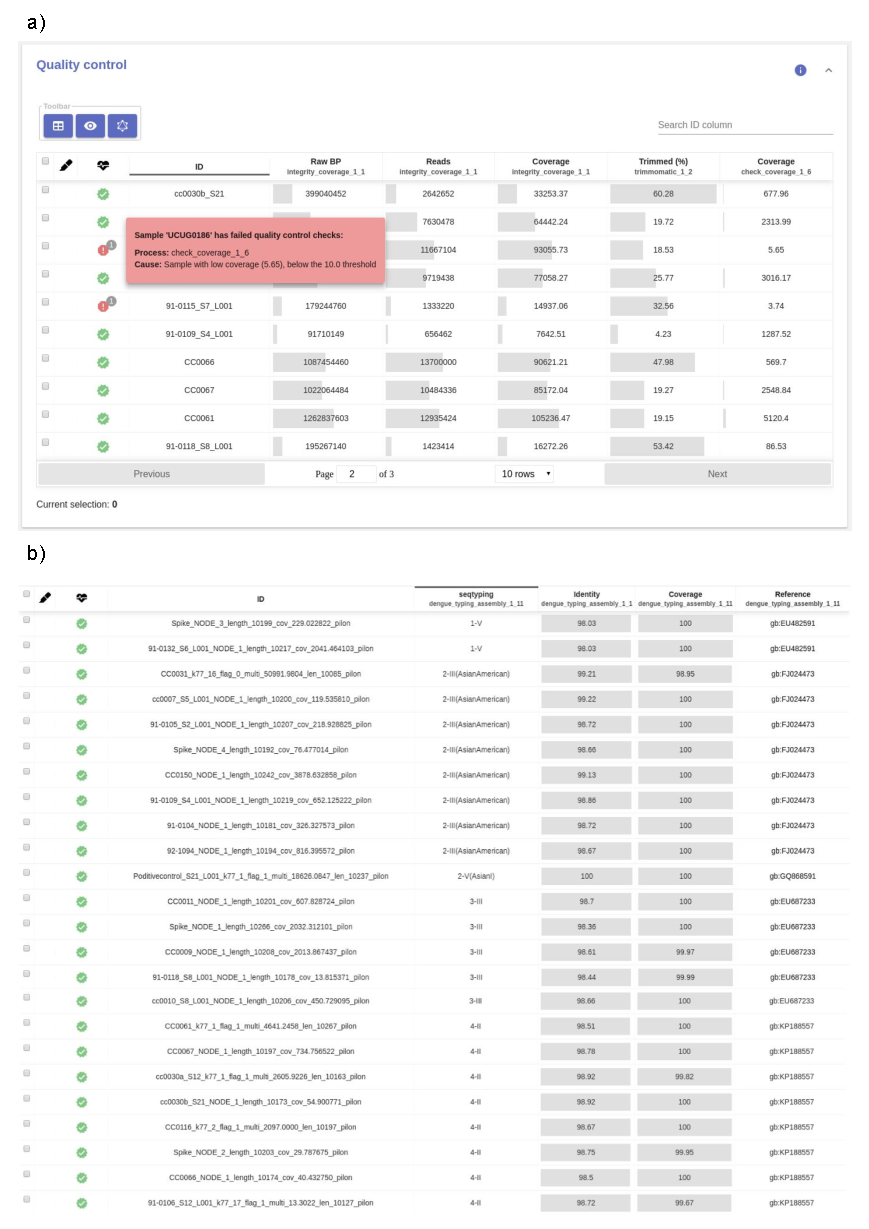
\includegraphics[width=\textwidth]{figures/chapter 4/Figure S1.pdf}
\caption{DEN-IM report tables. a) DEN-IM's quality control report containing information of the number of base-pairs and the number of reads for the analysed samples, the estimated coverage depth before and after mapping, and the percentage of reads in the input data that were trimmed. b) DEN-IM's typing report for 24 CDSs recovered from the metagenomic dataset. The ID contains the CDS contig name, the typing result for serotype-genotype, the values for identity and coverage, and the GenBank ID of the closest reference in the Typing Database containing 161 complete DENV genomes.}
\label{fig:chap4_figure_sup1}
\end{figure*}

\begin{figure*}[h!]
\centering
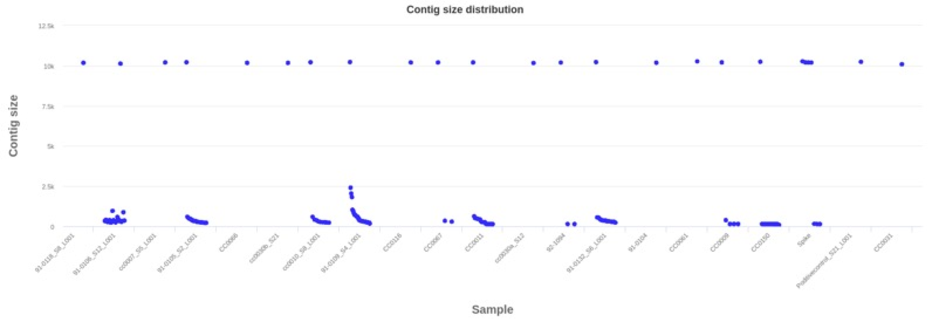
\includegraphics[width=\textwidth]{figures/chapter 4/Figure S2.pdf}
\caption{Contig size distribution for the shotgun metagenomics sequencing dataset. Each dot depicts an assembled DENV contig.  Above the 10Kb are full CDS of DENV.}
\label{fig:chap4_figure_sup2}
\end{figure*}

\begin{figure*}[h!]
\centering
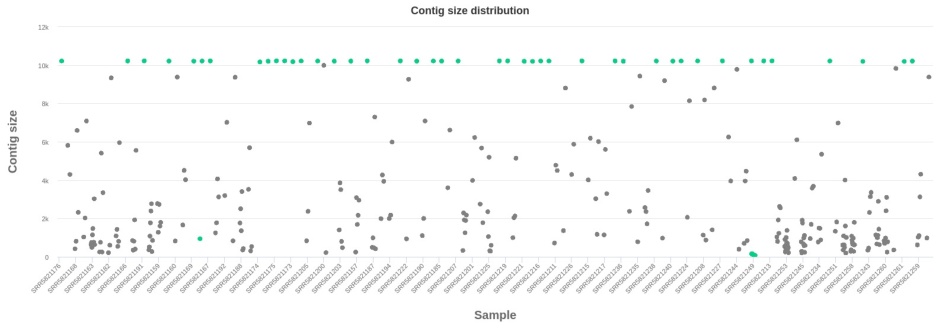
\includegraphics[width=\textwidth]{figures/chapter 4/Figure S3.pdf}
\caption{Contig size distribution of the amplicon sequencing dataset with 106 paired-end samples. Each dot depicts an assembled DENV contig. Above the 10Kb are full CDS of DENV. Contigs belonging from samples that assembled a complete DENV CDS are highlighted in green, whereas the remaining are coloured in grey.}
\label{fig:chap4_figure_sup3}
\end{figure*}

\begin{figure*}[h!]
\centering
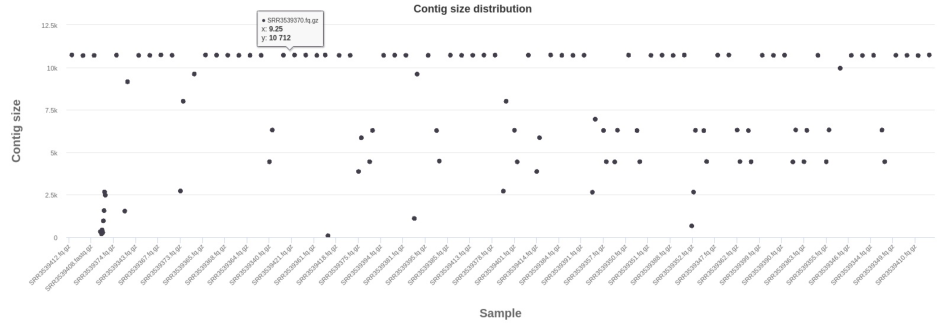
\includegraphics[width=\textwidth]{figures/chapter 4/Figure S4.pdf}
\caption{Contig size distribution of the amplicon sequencing dataset with 78 single-end samples. Each dot depicts an assembled DENV contig. Above the 10Kb are full CDS of DENV.}
\label{fig:chap4_figure_sup4}
\end{figure*}

\begin{figure*}[h!]
\centering
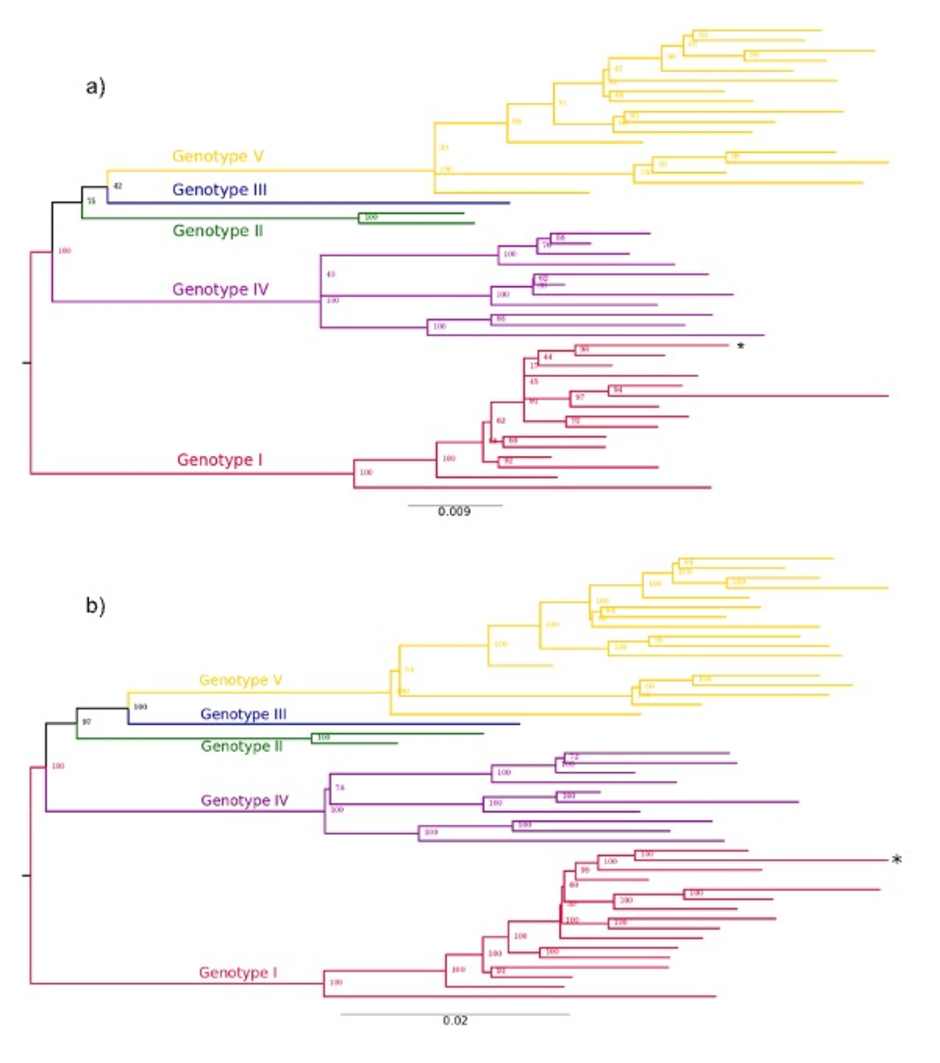
\includegraphics[width=\textwidth]{figures/chapter 4/Figure S5.pdf}
\caption{Maximum Likelihood inference of the multiple sequence alignment of the 46 DENV-1 complete genomes in the typing dataset, with a) envelope region and b) whole genome sequence. 1635 complete DENV-1 genomes were clustered at 98\% nucleotide identity and the representative genomes were aligned with MAFFT. A maximum likelihood tree was inferred with RAxML. The tree is coloured according to genotype (red: genotype I; green: genotype II; blue: genotype III; purple: genotype IV). The sample JF459993, marked with a star, is currently annotated in ViPR as belonging to genotype IV but, given to the good phylogenetic support, it was re-classified as belonging to the genotype I.}
\label{fig:chap4_figure_sup5}
\end{figure*}

\begin{figure*}[h!]
\centering
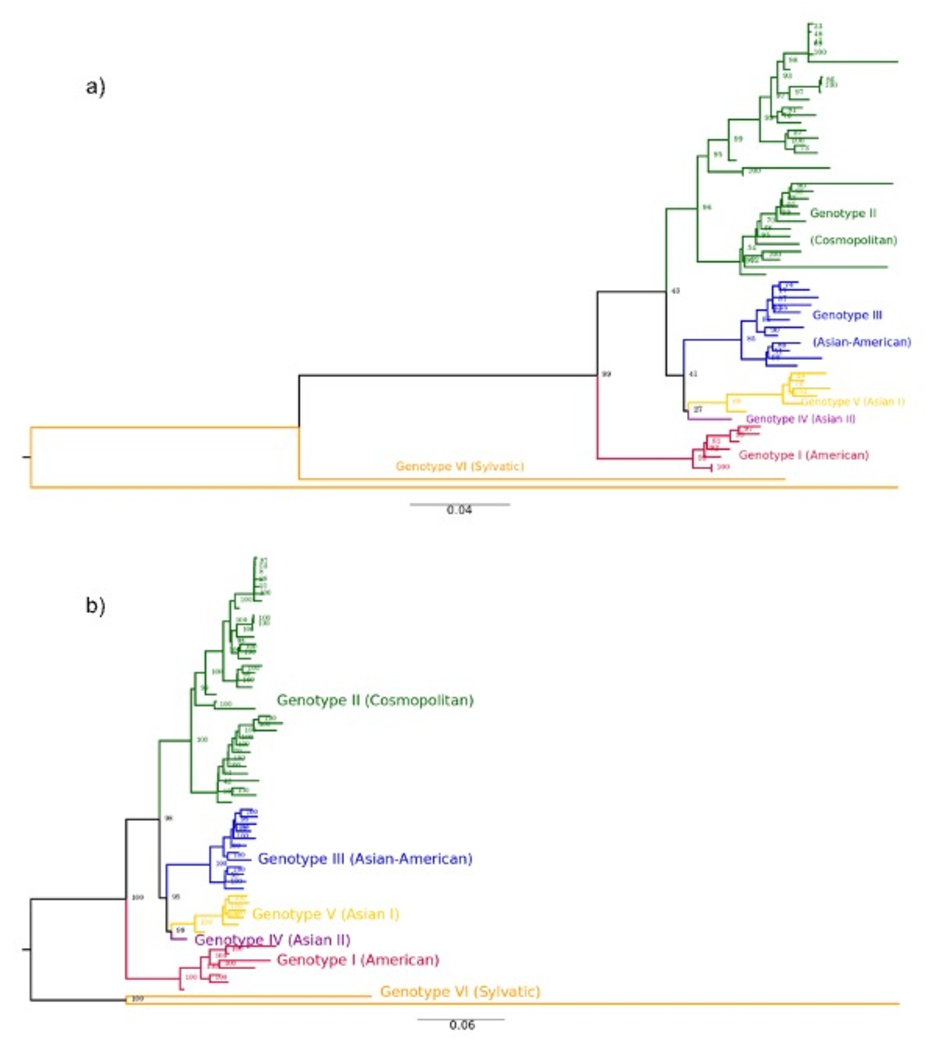
\includegraphics[width=\textwidth]{figures/chapter 4/Figure S6.pdf}
\caption{Maximum Likelihood inference of the multiple sequence alignment of the 63 DENV-2 complete genomes in the typing dataset, with a) envelope region and b) whole genome sequence. 1067 complete DENV-1 genomes were clustered at 98\% nucleotide identity and the representative genomes were aligned with MAFFT. A maximum likelihood tree was inferred with RAxML. The tree is coloured according to genotype (red: genotype I; green: genotype II; blue: genotype III; purple: genotype IV).}
\label{fig:chap4_figure_sup6}
\end{figure*}

\begin{figure*}[h!]
\centering
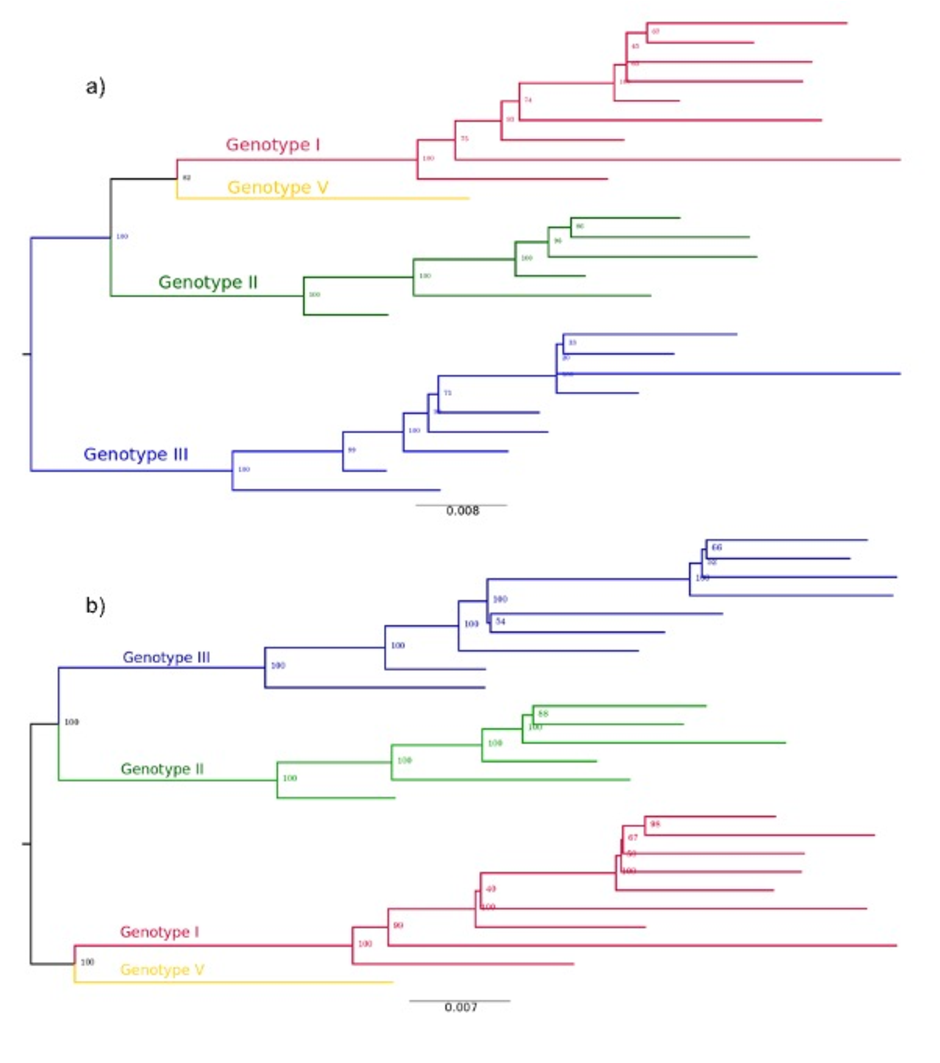
\includegraphics[width=\textwidth]{figures/chapter 4/Figure S7.pdf}
\caption{Maximum Likelihood inference of the multiple sequence alignment of the 25 DENV-3 complete genomes in the typing dataset, with a) envelope region and b) whole genome sequence. 807 complete DENV-3 genomes were clustered at 98\% nucleotide identity and the representative genomes were aligned with MAFFT. A maximum likelihood tree was inferred with RAxML. The tree is coloured according to genotype (red: genotype I; green: genotype II; blue: genotype III; purple: genotype IV).}
\label{fig:chap4_figure_sup7}
\end{figure*}

\begin{figure*}[h!]
\centering
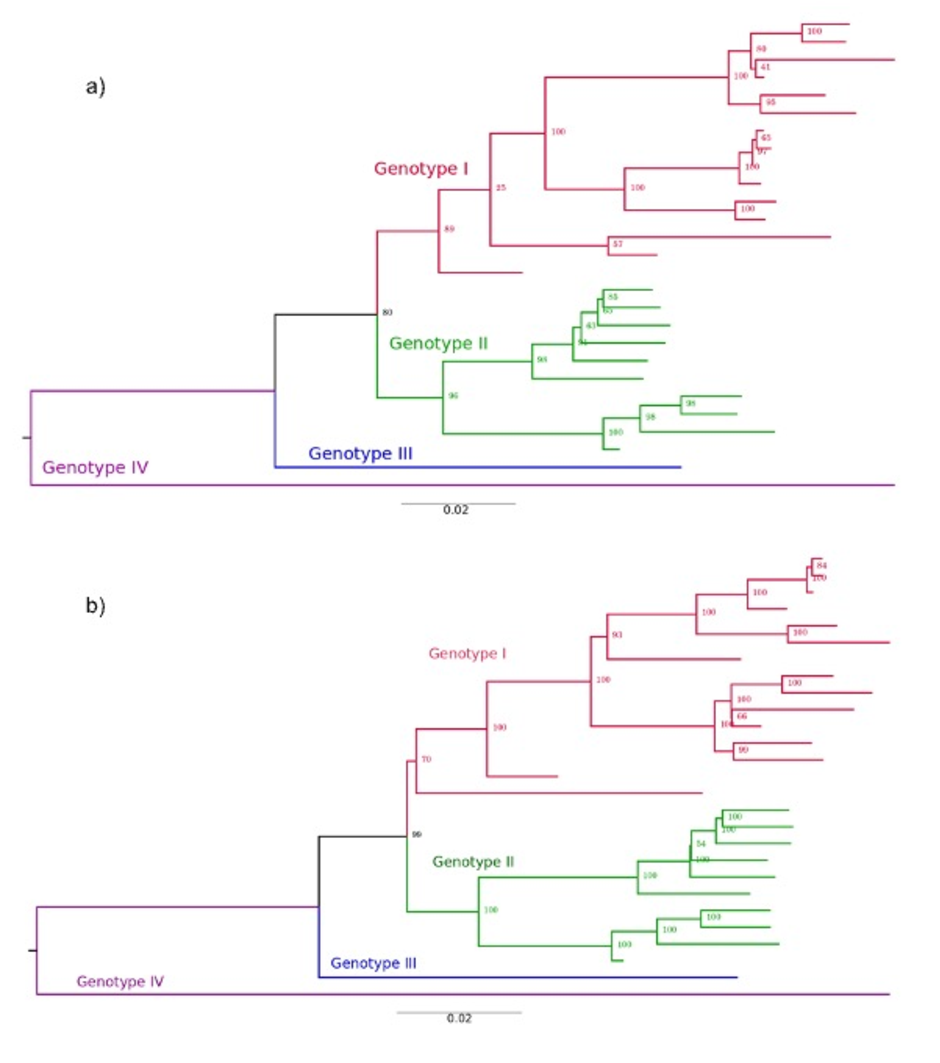
\includegraphics[width=\textwidth]{figures/chapter 4/Figure S8.pdf}
\caption{Maximum Likelihood inference of the multiple sequence alignment of the 27 DENV-4 complete genomes in the typing dataset, with a) envelope region and b) whole genome sequence. 320 complete DENV-4 genomes were clustered at 98\% nucleotide identity and the representative genomes were aligned with MAFFT. A maximum likelihood tree was inferred with RAxML. The tree is coloured according to genotype (red: genotype I; green: genotype II; blue: genotype III; purple: genotype IV).}
\label{fig:chap4_figure_sup8}
\end{figure*}
\newpage
\section{References}
\printbibliography[heading=none]
\end{refsection}

%-----------------------------------------------------------------
% Paper 4 - LMAS
%------------------------------------------------------------------
\newpage
\thispagestyle{empty}
\chapter{LMAS: Last Metagenomic Assembler Standing\label{ch:paper4}}

\thispagestyle{empty}
\clearpage \thispagestyle{empty}\mbox{}\clearpage
\newpage
\begin{refsection}
\mbox{}\\
\vspace{8cm}

This chapter is a reproduction of the following manuscript:

C. I. Mendes, P. Vila-Cerqueira, Y. Motro, J. Moran-Gilad, J. A. Carriço, M. Ramirez. LMAS: Evaluating metagenomic short de novo assembly methods through defined communities. GigaScience, Volume 12, 2023, giac122, \url{https://doi.org/10.1093/gigascience/giac122}

The supplementary information referred throughout the text can be consulted in this chapter before the section of references.

Short-read \ac{SMg} can offer comprehensive microbial detection and characterisation of complex clinical samples. The \textit{de novo} assembly of raw sequence data is key in metagenomic analysis, yielding longer sequences that offer contextual information and afford a more complete picture of the microbial community. The assembly process is the bedrock and may constitute a major bottleneck in obtaining trustworthy, reproducible results.

In this chapter, we present LMAS, an automated workflow developed as a flexible platform to allow users to evaluate traditional and metagenomic dedicated prokaryotic de novo assembly software performance given known standard communities. Its implementation in Nextflow ensures the transparency and reproducibility of the results obtained and the use of Docker containers provides further flexibility. The results are presented in an interactive HTML report where global and reference-specific performance metrics can be explored. Currently, 12 assemblers still being maintained are implemented in LMAS, with the possibility of expansion as novel algorithms are developed.

To showcase LMAS we initially used a test dataset of eight bacterial genomes and four plasmids of the ZymoBIOMICS Microbial Community Standards with linear and logarithmic distribution and found that k-mer De Bruijn graph assemblers outperformed the alternative approaches but came with a greater computational cost. Furthermore, assemblers branded as metagenomic specific did not consistently outperform other genomic assemblers in metagenomic samples. Some assemblers still in use, such as ABySS, MetaHipmer2, minia and VelvetOptimiser,  showed significant performance problems and their usability may be limited, particularly when assembling complex samples. 

To test assembler performance with an even more complex dataset, we used the 12-strain BMock12 community standard. This sample includes a non-even distribution of species and several closely related sets: two replicons of Halomonas sp. (ANIb=0.98), three replicons of the Micromonospora genus (average ANIb=0.85) and two replicons of Marinobacter sp (ANIb=0.78). Furthermore, and to represent a mock community trying to reproduce an existing microbiome, the NIBSC Gut DNA Reference Gut-Mix-RR and Gut-Mix-HiLo community standards were analysed, consisting of 20 common gut microbiome strains in an even and staggered composition respectively.

The performance of each assembler varied depending on the species of interest and its abundance in the sample, with less abundant species presenting a significant challenge for all assemblers. No assembler stood out as an undisputed all-purpose choice for short-read metagenomic prokaryote genome assembly, highlighting that efforts are still needed to further improve metagenomic assembly performance. Our results also suggest that sample complexity and a particular interest in some sample components may affect assembler choice. Using LMAS could help users in their choice of assembler for their specific purpose.  As such, we believe that this manuscript is appropriate for publication in Microbiome as a Software article. 

My contribution to this publication included the design, implementation and optimisation of the LMAS workflow, including the creation of the Docker containers for all dependencies. I performed the data analysis and comparison of assemblers included in LMAS with ZymoBIOMICS Microbial Community Standards, both evenly and logarithmically distributed samples, BMock12 and IBSC Gut DNA Reference Gut-Mix-RR and Gut-Mix-HiLo community standards. Additionally, I've also written the manuscript.

\cleardoublepage 

\begin{center}
\large
\textbf{LMAS: Evaluating metagenomic short de novo assembly methods through defined communities}
\end{center}

Catarina I. Mendes$^1,*$, 
Pedro Vila-Cerqueira$^1*$,
Yair Motro$^2$,
Jacob Moran-Gilad$^2$,
João A. Carriço$^1$
Mário Ramirez$^1$, 


$^1$Instituto de Microbiologia, Instituto de Medicina Molecular, Faculdade de Medicina, Universidade de Lisboa, Lisboa, Portugal 

$^2$Faculty of Health Sciences, Ben-Gurion University of the Negev, Beer-Sheva, Israel

\section{Abstract}

\textbf{Background }The de novo assembly of raw sequence data is key in metagenomic analysis. It allows recovering draft genomes from a pool of mixed raw reads, yielding longer sequences that offer contextual information and provide a more complete picture of the microbial community.

\textbf{Results} To better compare de novo assemblers for metagenomic analysis, LMAS was developed as a flexible platform allowing users to evaluate assembler performance given known standard communities. Overall, in our test datasets, k-mer De Bruijn graph assemblers outperformed the alternative approaches but came with a greater computational cost. Furthermore, assemblers branded as metagenomic specific did not consistently outperform other genomic assemblers in metagenomic samples. Some assemblers still in use, such as ABySS, MetaHipmer2, minia and VelvetOptimiser, perform relatively poorly and should be used with caution when assembling complex samples. 

\textbf{Conclusions} The choice of a de novo assembler depends on the computational resources available, the replicon of interest, and the major goals of the analysis. No single assembler appeared an ideal choice for short-read metagenomic prokaryote replicon assembly, each showing specific strengths. The choice of metagenomic assembler should be guided by user requirements and characteristics of the sample of interest, and LMAS provides an interactive evaluation platform for this purpose. 

\subsubsection{Keywords}

Shotgun Metagenomics, de novo assembly, benchmark, draft genome quality, simulation

\section{Background}

Short-read shotgun metagenomics has the potential to offer comprehensive microbial detection and characterisation of complex clinical or environmental samples.  Despite becoming an increasingly used approach, it comes at the cost of producing massive amounts of data that require expert handling and processing, as well as adequate computational resources. The \textit{de novo} assembly process is key when analysing metagenomic data since it allows recovering contigs representing the replicons present in the sample, be it prokaryotic chromosomes, plasmids or viruses, from a pool of mixed raw reads. These contigs are longer sequences that offer better contextual information than reads alone and provide a more complete picture of the microbial community than the species composition. Despite efforts for the development, standardisation and assessment of software for metagenomic analysis, both commercial and open-source \cite{angers-loustau_challenges_2018,gruening_recommendations_2019, sczyrba_critical_2017, couto_critical_2018, meyer_critical_2021}, the de novo assembly process still represents a critical point in these analyses.

The assembly of draft genomes has become a central step when analysing pure bacterial cultures, for instance allowing genomic comparisons through single nucleotide \ac{SNP}s or gene-by-gene methods, such as \ac{cgMLST}. De Bruijn graphs (dBg) algorithms are currently the most widely used approach in modern assembly software. dBg handles unresolvable repeats by essentially fragmenting the sequence, that is, forming multiple contigs for each of the possibly contiguous sequences present in the sample. Additionally, the inherent heterogeneity of complex samples, potentially containing a multitude of replicons, could make traditional genome assemblers, implementing optimisations based on the assumption of having a single genome in the sample, not suitable for metagenomics \cite{ayling_new_2020}.

Several dedicated metagenomic assembly tools for short-read data are available \cite{ayling_new_2020}. These tools are generally assumed to perform better when dealing with complex samples having a combination of intragenomic and intergenomic repeats and uneven and low coverage sequencing depths of some of the replicons \cite{olson_metagenomic_2019}. Not using dedicated metagenomic assemblers was suggested to come with the cost of generating artificial variation and chimeric contigs, especially in samples that contain closely related species \cite{teeling_current_2012}. However, to our knowledge, no formal comparison has been done looking at increased accuracy or gains in contiguity of assemblies obtained with metagenomic assemblers versus traditional assemblers.

With an ever-increasing range of both traditional and metagenomic assemblers becoming available, choosing the best performing tool can be an arduous and time-consuming task since the choice may vary depending on the purpose of the analysis, organism of interest, complexity of the sample and computational infrastructure available. Additionally, the evaluation of the resulting contigs is not straightforward since one metric is not sufficient to classify an assembly, particularly with complex samples \cite{olson_metagenomic_2019,bradnam_assemblathon_2013}. Despite several de novo assembly validation methods relying on features of the created contigs themselves, such as QUAST \cite{gurevich_quast_2013}, being useful in identifying inconsistencies indicative of potential assembly errors, the use of reference-based validation methods offer the possibility of a more complete evaluation of accuracy and are particularly important to benchmark attempts to reconstruct communities. MetaQUAST \cite{bradnam_assemblathon_2013}, a modification of QUAST, extends the original software by performing assembly evaluation based on aligning contigs to a reference, which can be provided or inferred by the software, and reports, in addition to the standard metrics for single genomes reported by QUAST, the number of interspecies translocations and the number of possibly misassembled contigs.

The use of mock communities, with known composition, abundance and genomic information, provides a ground truth against which the success of the assembly of a complex sample can be evaluated. Such mock communities facilitate the identification of misassemblies, such as chimeric sequences generated from the improper combination of two distinct replicons, indels or single nucleotide variants improperly created by the assembler. On the other hand, the comparison of the performance of two assemblers is only possible if the input data is the same and if the same evaluation metrics are applied \cite{sczyrba_critical_2017}. 

To tackle these challenges, we developed LMAS (Last Metagenomic Assembler Standing), an automated workflow to enable the benchmarking of traditional and metagenomic prokaryotic de novo assembly software using defined mock communities. The results of LMAS are presented in an interactive HTML report where selected global and reference replicon-specific performance metrics can be explored. The mock communities can be provided by the user to better reflect the samples of interest. New assemblers can be added with minimal changes to the pipeline so that LMAS can be expanded to include novel algorithms as they are developed. The portability and ease of use of LMAS are intended to allow provide users with a continuous benchmarking platform to easily evaluate the performance of assemblers, in mock communities mimicking as closely as possible their samples of interest.

\section{Implementation}

\subsection{Workflow overview}

LMAS is a user-friendly automated workflow enabling the benchmarking of traditional and metagenomic prokaryotic de novo assembly software using defined mock communities. LMAS was implemented in Nextflow \cite{di_tommaso_nextflow_2017} to provide flexibility and ensure the transparency and reproducibility of the results. LMAS relies on the use of Docker \cite{merkel_docker_2014} containers for each assembler, allowing versions to be tracked and changed easily.

\begin{figure*}[]
\centering
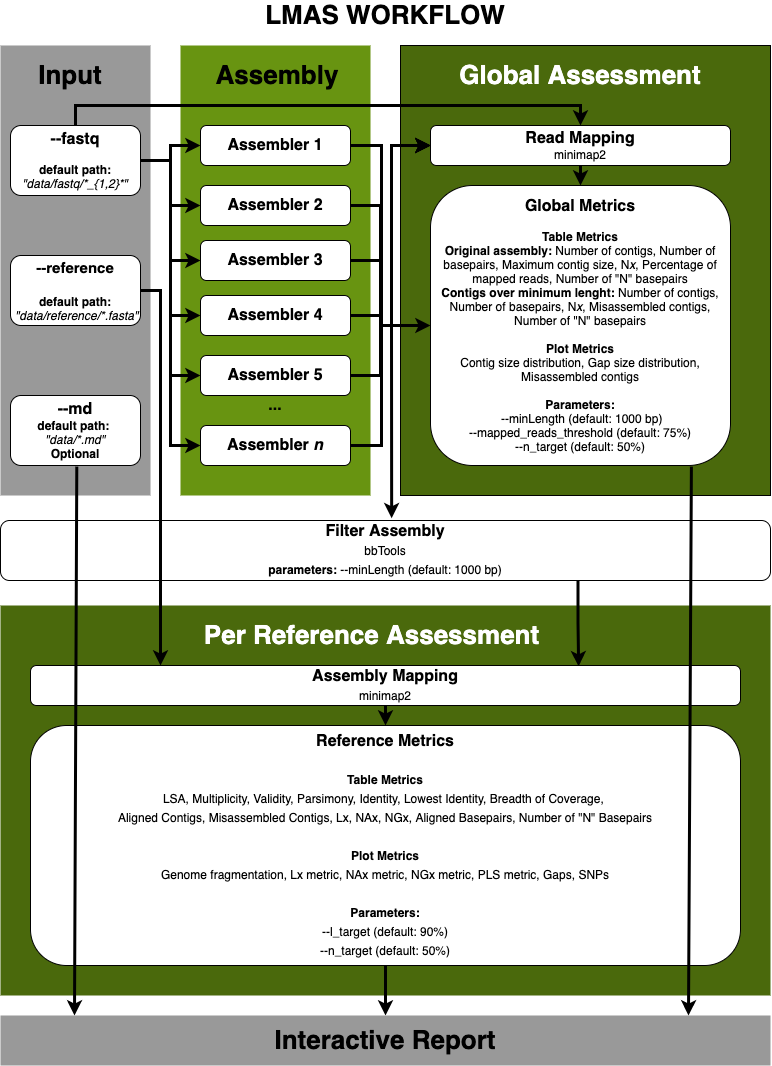
\includegraphics[width=\textwidth]{figures/chapter 5/Figure 1.png}
\caption{The LMAS workflow. The input sequencing data is assembled in parallel, resources permitting, by the set of assemblers included in LMAS. The resulting contigs are processed and the global quality assessment is performed. After filtering for the user-defined minimum contig size, the remaining sequences are mapped against the provided reference and the resulting information is processed to evaluate assembly quality by replicon in the reference file. All results, and optional text information describing the samples, are grouped in the LMAS report.}
\label{fig:chap5_figure1}
\end{figure*}

\subsection{Installation and Usage}

LMAS can be installed through Bioconda \cite{noauthor_lmas_nodate} or Github \cite{mendes_lmas_2021}, with detailed instructions available in the documentation \cite{noauthor_installation_nodate}. LMAS requires as inputs the complete reference replicons (genomes, plasmids or any other replicons present) and short-read paired-end raw data. All complete references (linear replicons) should be provided in a single file. This raw data can be either obtained in silico by creating simulated reads from the reference replicons or sequencing mock communities of known composition. Optionally, information on the input samples in a markdown file can be provided to be presented in the report.

A step-by-step execution tutorial is available at \cite{noauthor_basic_nodate}. Users can customise the workflow execution either by using command-line options or by modifying the simple plain-text configuration files. To make the execution of the workflow as simple as possible, a set of default parameters and directives is provided. A complete description of each parameter is available in Supplemental Material (see Supplemental Material, Workflow parameters), as well as in the documentation \cite{noauthor_parameters_nodate}.  The results are presented in an interactive HTML report, stored in the “report” folder in the directory of LMAS’ execution. The output files of all assemblers and quality assessment processing scripts in the workflow are stored in the “results” folder, in the same location. 

\subsection{Supported Assemblers and selection criteria}

A collection of de novo assembly tools was compiled, including \ac{OLC} and \ac{dBg} assembly algorithms, the latter including both single k-mer and multiple k-mer value approaches, and hybrid assemblers implementing both algorithms, including both genomic and metagenomic assemblers (Supplemental Table \ref{tab:ch5_suptable1}).Of these, 11 assemblers were selected based on the date of last update (at least 2015) and are implemented in LMAS: ABySS \cite{jackman_abyss_2017} (version 2.3.1), GATB Minia Pipeline \cite{noauthor_gatbgatb-minia-pipeline_2022} (commit hash 9d56f42) , IDBA-UD \cite{peng_idba-ud_2012} (version 1.1.3), MEGAHIT \cite{li_megahit_2015} (version 1.2.9), MetaHipMer2 \cite{georganas_extreme_2018} (version 2.0.0.65-gaad446d-dirty-AddGtest), metaSPAdes \cite{nurk_metaspades_2017} (version 3.15.3), minia \cite{chikhi_space-efficient_2013} (version 3.2.6), SKESA \cite{souvorov_skesa_2018} (version 2.5.0), SPAdes \cite{bankevich_spades_2012} (version 3.15.3), Unicycler \cite{wick_unicycler_2017} (version 0.4.9) and VelvetOptimiser \cite{seemann_velvetoptimiser_2021} (commit hash 092bdee) (Table \ref{tab:ch5_table1}). The execution commands for each assembler are available as Supplemental Material (see \ref{ch5_sup_assemblers}) and in the documentation \cite{noauthor_short-read_nodate}. 
New assemblers can be added with minimal changes to the pipeline so that LMAS can be expanded as novel algorithms are developed. A template is available to facilitate their integration and a step-by-step guide is included in the documentation \cite{noauthor_add_nodate}. The only two requirements for the addition of a new assembler are the execution command for the assembler for paired-end short-read data and a Nextflow-compatible container with the assembler and any dependencies.

\begin{scriptsize}
\begin{center}

\begin{table}[]
\centering
\caption{Prokaryotic de novo assemblers integrated into LMAS.}
\label{tab:ch5_table1}
\begin{tabular}{@{}lll@{}}
\toprule
Assembler         & Type        & Algorithm                        \\ \midrule
GATBMiniaPipeline & Metagenomic & Multiple   k-mer De Bruijn graph \\
IDBA-UD           & Metagenomic & Multiple   k-mer De Bruijn graph \\
MEGAHIT           & Metagenomic & Multiple   k-mer De Bruijn graph \\
MetaHipMer2       & Metagenomic & Multiple   k-mer De Bruijn graph \\
metaSPAdes        & Metagenomic & Multiple   k-mer De Bruijn graph \\
ABySS             & Genomic     & Single   k-mer De Bruijn graph   \\
BCALM2            & Genomic     & Single   k-mer De Bruijn graph   \\
MINIA             & Genomic     & Single   k-mer De Bruijn graph   \\
SKESA             & Genomic     & Multiple   k-mer De Bruijn graph \\
SPAdes            & Genomic     & Multiple   k-mer De Bruijn graph \\
Unicycler         & Genomic     & Multiple   k-mer De Bruijn graph \\
VelvetOptimizer   & Genomic     & Multiple   k-mer De Bruijn graph \\ \bottomrule
\end{tabular}
\end{table}

\end{center}
\end{scriptsize}


\subsection{Assembly Quality Metrics}

The success of an assembly is evaluated in two steps: globally (see \ref{sssec:_chap5_global_metrics}) and relative to each of the replicons present in the sample (see \ref{sssec:_chap5_reference_metrics}). In both, the tabular presentation in the reports allows the comparison of exact values between assemblers, and the interactive plots allow a more intuitive overview and easy exploration of results. In addition to the assembly success metrics, computational resource statistics are registered for each assembler (see \ref{ch5_sup_performance_metrics}).

\subsubsection{Global Metrics} \label{sssec:_chap5_global_metrics} 

The computation of the global metrics is performed through statistics inherent to the complete set of contigs assembled per sample, independent of the species/sample of origin. The metrics are presented, in tabular form, for the complete set of contigs and those filtered for a minimum length, and also graphically for the contigs filtered for a minimum length. The statistics include information on contig number, size and ambiguous bases; and the proportion of reads mapping to the created contigs. Two statistics are a consolidation of per reference metrics: misassemblies (i.e. contigs that do not reflect the structural organisation in the reference replicons); and the overall size of gaps in all reference replicons not covered by any contig. A more detailed description of all global metrics is available in Supplemental Material (see \ref{ch5_supmaterial_metrics_global}). 

\subsubsection{Per Reference Metrics} \label{sssec:_chap5_reference_metrics} 

For the computation of the reference-based metrics, only the \ac{FS} contigs are considered, for each reference replicon in the sample. These contigs are the ones exceeding the user-defined minimum sequence length, filtered using BBTools (version 38.44). After this initial step, the contigs are mapped to the reference replicons with minimap2 \cite{li_minimap2_2018} (version 2.22). The metrics are computed through custom python code (see \ref{ch5_sup_assembly_filtering_and_mapping}) for each replicon in the file provided as input. A detailed description of all reference-based metrics is available in Supplemental Material (see \ref{ch5_supmaterial_metrics_reference}). 

In addition to the statistics shared with the global metrics, LMAS also calculates the number of mismatches relative to each reference, the COMPASS \cite{earl_assemblathon_2011} metrics and two new metrics we propose: \ac{LSA} and \ac{Pls}.

\ac{LSA} represents the fraction of the longest single alignment between a contig and the reference, relative to the reference length. The \ac{Pls}, or Phred-like score, is a scoring function based on the identity of each aligned contig to the reference replicon. Similarly to the Phred quality score \cite{ewing_base-calling_1998}, a measure of the quality of the identification of the bases by sequencing, the \ac{Pls} measures the quality of the assembly of a contig. The formula of \ac{Pls} is similar to the Phred score formula but uses as the error function the identity of the base in the contig to that of the reference replicon. The formula to obtain the \ac{Pls} metric per contig is Equation \ref{ch5_eq1}. 

\begin{equation} \label{ch5_eq1}
    Phred(E) = \left\{\begin{matrix}
-log(E)\times 10 & \textup{if } 0 < E \leq 1\\
 60 & \textup{if }E = 0
\end{matrix}\right. \\
\textup{ where }E = 1-\textup{Identity}
\end{equation}

\subsection{The LMAS Report}

The LMAS results are presented in an interactive HTML. The LMAS report is composed of two main panels: a top summary panel with information on input samples (provided by the user) and the resources used during LMAS’ execution, and a bottom panel where selected global and reference specific assembly metrics can be explored for each sample. LMAS constructs the HTML file after workflow completion, storing it in the “reports” folder. The report data can be easily shared between users and requires only a browser for visualisation.

\begin{figure*}[h!]
\centering
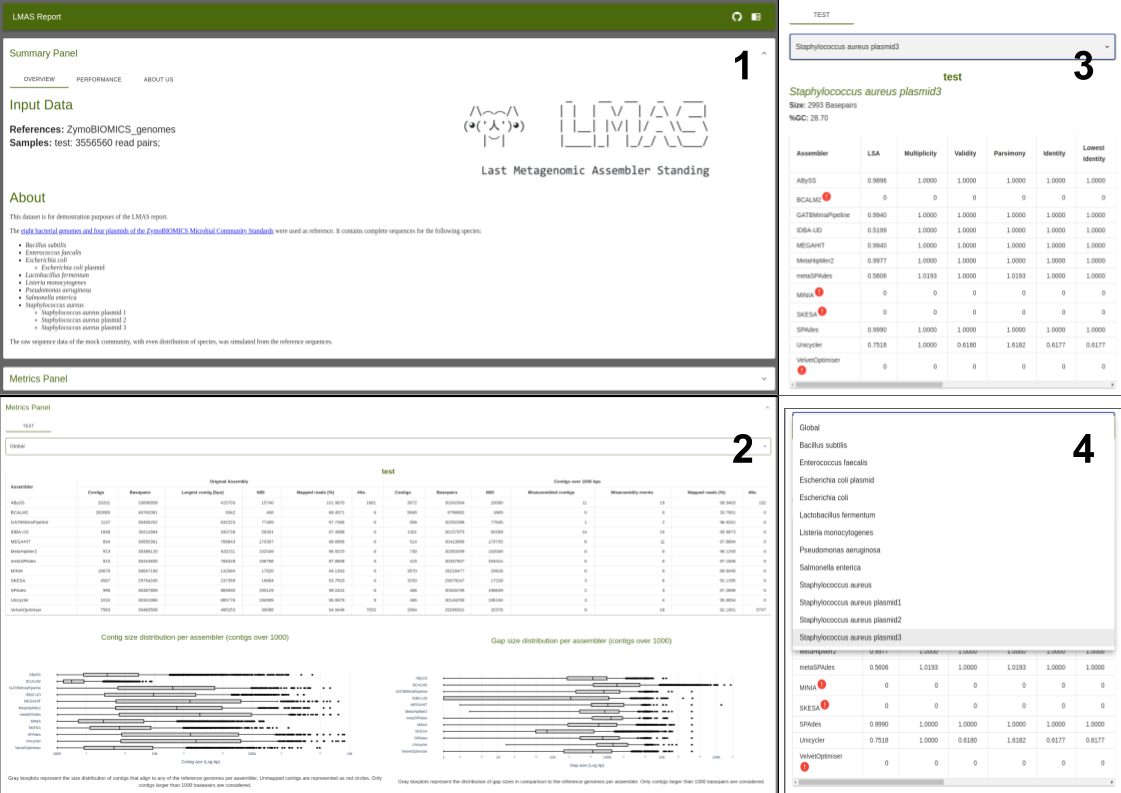
\includegraphics[width=\textwidth]{figures/chapter 5/Figure 2.png}
\caption{The LMAS report.  All results, and optional text information describing the samples, are grouped in the LMAS report, an interactive and responsive HTML file,  for exploration in any browser. Links for LMAS source code and documentation are available in the top right corner of the report. 1) The summary panel of the LMAS report contains information on the input reference sequences and raw sequencing data samples (provided by the user), and the overall computational performance of the assemblers in LMAS. 2) The LMAS metric panel contains the explorable global and reference specific performance metrics per input raw sequencing data sample.  The tabular presentation allows direct comparison of exact values between assemblies, and the interactive plots allow for an intuitive overview and easy exploration of results. 3) If an assembler fails to produce an assembly, or fails to assemble sequences that map to the reference replicon, it is marked in the table with a red warning sign. 4) The global or reference replicon specific metrics can be accessed for each sample in the dropdown menu.}
\label{fig:chap5_figure2}
\end{figure*}

\subsubsection{Summary Panel} \label{sssec:_chap5_summary_panel}

The top panel of the report contains information on the input samples and overall performance of the assemblers in LMAS, divided into three tabs:  Overview, Performance and About us. On the top right corner of the report, direct links to LMAS’ source repository and documentation are provided.

\begin{itemize}
    \item \textit{Overview}: This tab contains information on the input data, including the name and number of reads of the raw sequencing data, and the name of the reference file. Additional information provided by the user about the community used as input is also presented here. 
    \item \textit{Performance}: This tab contains a table with information on the version, the containers used and computational performance metrics for each assembler in LMAS.
    \item\textit{ About us}: This tab contains information on the LMAS GitHub repositories and the LMAS development team. 
\end{itemize}

\subsubsection{Metrics Panel} \label{sssec:_chap5_summary_panel} 

The bottom portion of the report contains the explorable global and reference specific performance metrics per input raw sequencing data sample. Each sample has its own tab and the global or reference replicon specific metrics can be accessed in the dropdown menu. 


\paragraph{Global Metrics} \label{sssec:_chap5_summary_panel_global} \mbox{}\\

A table displays the global assembly metrics computed for the complete and \ac{FS} contigs. If an assembler fails to produce an assembly, it is marked on the table with a red warning sign. The global metric plots are interactive, allow zooming in on particular areas and provide extra information as hover text boxes. The plots can be saved as PNG in whatever view the user selects. 

\paragraph{Per Reference Metrics} \label{sssec:_chap5_summary_panel_reference} \mbox{}\\

Similarly to the global assembly metrics, a table displays the computed set of reference restricted metrics for the \ac{FS} contigs. If an assembler fails to produce sequences that align to the reference, these are marked in the table with a red warning sign. Information on the expected reference replicon length and the GC content is calculated from the input files and reported above the table. The per-reference metric plots are also interactive, allowing the same type of operations as the global metric plots. 

\subsection{Comparison with other assembly evaluation software programs}

The assessment and evaluation of genome assemblies has been a relevant field ever since the emergence of the assembly process itself, and therefore many solutions have been proposed \cite{sczyrba_critical_2017, olson_metagenomic_2019, bradnam_assemblathon_2013, gurevich_quast_2013, mikheenko_metaquast_2016, manchanda_genomeqc_2020, meader_genome_2010, challis_blobtoolkit_2020}. The Critical Assessment of Metagenome Interpretation (CAMI) proposed a set of recommendations and best practices for benchmarking in microbiome research \cite{meyer_tutorial_2021}. These recommendations include the reporting of computational performance, which may condition the choice of software by the users, such as runtime, disk space and memory consumption, also reported by  LMAS (see \ref{ch5_supmaterial_metrics}). As also suggested by CAMI, LMAS tracks the exact program version and command-line calls through its implementation in Nextflow. Moreover,  using containerised assemblers and being easily installable through Bioconda, LMAS facilitates deployment in diverse user machines. Unlike the CAMI tutorial, in which users are asked to download and install the necessary tools, in LMAS everything is provided in a one-stop reproducible workflow that effortlessly handles all pre-processing, assembly, post-processing, traceability and report production steps, freeing users to focus on providing relevant samples for analysis and interpreting the results in view of the intended applications.

Concerning software for assembly quality assessment currently available, the most widely adopted is QUAST \cite{gurevich_quast_2013}, or when dealing with metagenomic data, its extension metaQUAST \cite{mikheenko_metaquast_2016}, which was also adopted by the CAMI challenges [3,5] \cite{sczyrba_critical_2017, meyer_critical_2021} and suggested in the CAMI Tutorial \cite{meyer_tutorial_2021}. Although several features of these tools overlap with LMAS’ quality assessment components, these differ from LMAS in the sense that they are not a single step workflow allowing a traceable and reproducible assembly of mock communities. Unlike QUAST and metaQUAST, whose purpose is to evaluate assemblies, the purpose of LMAS is to allow users to evaluate assembler performance for a given sample of interest. Supplementary Table \ref{tab:ch5_suptable2} shows the comparison of the output and computed assembly quality metrics generated by LMAS, QUAST and metaQUAST. 

\section{Results and Discussion}

To illustrate the use of LMAS and evaluate the performance of the chosen assemblers we initially used the eight bacterial genomes and four plasmids of the ZymoBIOMICS Microbial Community Standards as reference. As input we used the raw sequence reads of mock communities with an even and logarithmic distribution of species, from real sequencing runs \cite{nicholls_ultra-deep_2019} and simulated read datasets, with and without error, matching the distribution of species in each sample \cite{gourle_simulating_2019}. Our dataset is composed of samples ENN (in silico generated evenly distributed without error), EMS (in silico generated evenly distributed with Illumina MiSeq error model), ERR2984773 (evenly distributed real Illumina MiSeq sample), LNN (in silico generated logarithmically distributed without error), LHS (in silico generated logarithmically distributed with Illumina HiSeq error model) and ERR2935805 (logarithmically distributed real Illumina HiSeq sample) (see Supplemental Table \ref{tab:ch5_suptable3}). Detailed information about the generation of the input samples is available as Supplemental Material (see \ref{ch5_sup_zymobiomics}, Supplemental Table \ref{tab:ch5_suptable4}). To evaluate the reproducibility of an assembler performance, the LMAS workflow was run three times for all samples using default parameters, and the resulting data was processed for each sample (see Chapter \ref{ch5_sup_assembly_success}) Supplementary Table \ref{tab:ch5_suptable5} to Table \ref{tab:ch5_suptable10} present an overview of the average global performance per assembler for each sample in LMAS. 

To test assembler performance with an even more complex dataset, we used the 12 strain BMock community standard (accession SRX4901583, real Illumina HiSeq 2500 sample) \cite{sevim_shotgun_2019}. This sample includes a non-even distribution of species, with the most abundant replicon having 3093x coverage (\textit{Muricauda} sp. ES.050) and the lowest only 0.1x coverage (\textit{Micromonospora coxensis}) (Supplementary Table \ref{tab:ch5_suptable24}). For the sake of a less resource-intense evaluation we downsampled to have 20\% of the reads available in the original sample and further processed only these. The main challenges of this data set are possibly to assemble the genomes of the three \textit{Micromonospora} spp. and the two \textit{Halomonas} spp. strains, which have an ANIb >0.84 and 0.98, respectively (Supplementary Table \ref{tab:ch5_suptable25}). The two \textit{Marinobacter} spp. have an ANIb of 0.78.

To represent more realistic samples of a human microbiome study, the Gut-Mix-RR and Gut-Mix-HiLo standards, including 20 species known to be present in the human gut, were used as reference (accessions SRR11487941 and SRR11487935, respectively, both real Illumina MiSeq samples) \cite{amos_developing_2020}. For the Gut-Mix-RR, the abundance of each bacterial genome is relatively even (maximum of 66x, an average of 22.32x and a minimum of 5.99x; Supplementary Table \ref{tab:ch5_suptable28}). The Gut-Mix-HiLo has an uneven abundance of species (maximum of 115x, an average of 20.45x and a minimum of 0.34x; Supplementary Table \ref{tab:ch5_suptable28}). The genomes in these mock communities are fairly diverse (average ANIb=0.67, Supplementary Table \ref{tab:ch5_suptable29}), with the two subspecies of \textit{Bifidobacterium longum} (ANIb=0.95) possibly being the most challenging. It is worth noting that only draft genomes are available for eight of the strains, including one of the \textit{Bifidobacterium longum} subspecies (Supplementary Table \ref{tab:ch5_suptable28}). The \textit{Roseburia hominis} and \textit{Roseburia intestinalis} are the closest related closed replicons (ANIb>0.77) in this sample.

\subsection{Some assemblers perform poorly}

Of the 12 de novo prokaryotic assemblers included in LMAS, 4 stand out as having an overall poor performance in the ZymoBIOMICS Microbial Community Standards dataset: ABySS, MetaHipmer2, minia and VelvetOptimiser. Both ABySS and MetaHipmer2 performed inconsistently with differing resource requirements for the same sample in different runs, namely run time and memory allocation (see \ref{ch5_sup_resources}, Supplemental Figure \ref{fig:chap5_sup_figure_2}).  Moreover, ABySS failed to produce an assembly for sample ERR2984773 for 1 of the runs (see Supplementary Table \ref{tab:ch5_suptable7}) and for sample LHS in any of the 3 runs in the time limit of 3 days (see Supplementary Table \ref{tab:ch5_suptable9}), and MetaHipmer2 failed to produce an assembly for samples LNN and LHS in all 3 runs (see Supplementary Tables \ref{tab:ch5_suptable8}-\ref{tab:ch5_suptable9}). VelvetOptimiser generated the highest number of inconsistent contigs across the 3 LMAS runs (Figure \ref{fig:chap5_figure3}, Supplementary Table \ref{tab:ch5_suptable11}), with 1.69\% of the total contigs created present in only 1 or 2 runs. Although not as extreme as VelvetOptimiser, ABySS (0.52\%), minia (0.14\%), GATBMiniaPipeline (0.32\%), MetaHipMer2 (0.11\%) and IDBA-UD (0.08\%) also showed inconsistencies in contig size.

\begin{figure*}[h!]
\centering
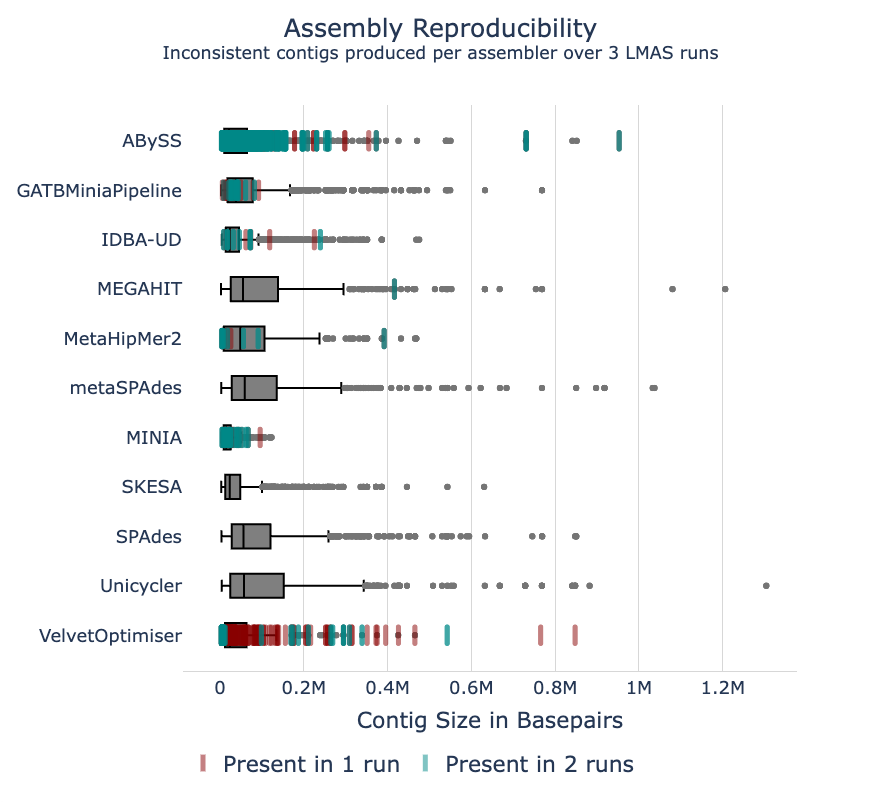
\includegraphics[width=\textwidth]{figures/chapter 5/Figure 3.png}
\caption{Assembly reproducibility. Inconsistent contigs produced per assembler over 3 LMAS runs. The distribution of contig sizes, in basepairs, consistently present in all three LMAS runs are indicated in the grey boxplots for each assembler. If an assembler produced a contig only present in two of the runs (as determined by its size), its size is indicated in teal. If a contig is present in a single run, it is represented in red.}
\label{fig:chap5_figure3}
\end{figure*}

Regarding the quality assessment of the assemblies produced (Figure \ref{fig:chap5_figure4}, Supplementary Table \ref{tab:ch5_suptable12}), ABySS and minia are the only single k-mer \ac{dBg} assemblers in the collection and were found to mostly underperform relative to their multiple k-mer \ac{dBg} counterparts, as reported previously \cite{sczyrba_critical_2017, meyer_critical_2022, xavier_employing_2014, mahadik_scalable_2019}, generally resulting in more fragmented assemblies, although there were significant differences in performance across samples. Among multiple k-mer assemblers, VelvetOptimiser frequently produced a very high number of contigs of very small size (over 99\% of the contigs not surpassing the minimum length of 1,000 \ac{bp}) and therefore a low N50 (an average of 29,768 \ac{bp} versus a global average of 84,114 \ac{bp}) (Supplementary Tables \ref{tab:ch5_suptable5}-\ref{tab:ch5_suptable10}). Additionally, ABySS and VelvetOptimizer produced contigs with a very large number of Ns, with an average of 1,019 and 3,035 uncalled bases per assembly, respectively. MetaHipMer2, although having overall average metrics in the two evenly distributed mock samples (ENN and EMS, Supplementary Tables \ref{tab:ch5_suptable5}-\ref{tab:ch5_suptable6}) where it was able to run successfully, it severely underperformed in the real samples (ERR2984773 and ERR2935805, Supplementary Tables \ref{tab:ch5_suptable7} and \ref{tab:ch5_suptable10}). Generally, the performance scores of the assemblers decreased considerably for the real samples in comparison with the simulated ones, either with or without error, underscoring the importance of using mock samples instead of simulated reads to evaluate assembler performance. High utilisation of the reads in the dataset is observed for most assemblers, with on average at least 90\% of the reads mapping back to the assembly, except for ABySS, MetaHipMer2 and VelvetOptimiser whose values are in the range of 46-79\%. Despite an overall good performance, SPAdes produced the highest number of misassembled contigs in the logarithmically distributed sample, with an average of 98 and a maximum of 572 (sample ERR2935805, Supplementary Table \ref{tab:ch5_suptable10}), in comparison to the global average of 11 misassembled contigs for all assemblers across all samples. However, this behaviour was not consistent across samples, with the evenly distributed sample showing similar misassembled contigs between SPAdes and other assemblers, similarly to the other mock samples tested (see below).

Due to their poor performance discussed above, the following assemblers have not been included in subsequent analyses: ABySS, MetaHipmer2, minia and VelvetOptimiser. 

\begin{figure*}[h!]
\centering
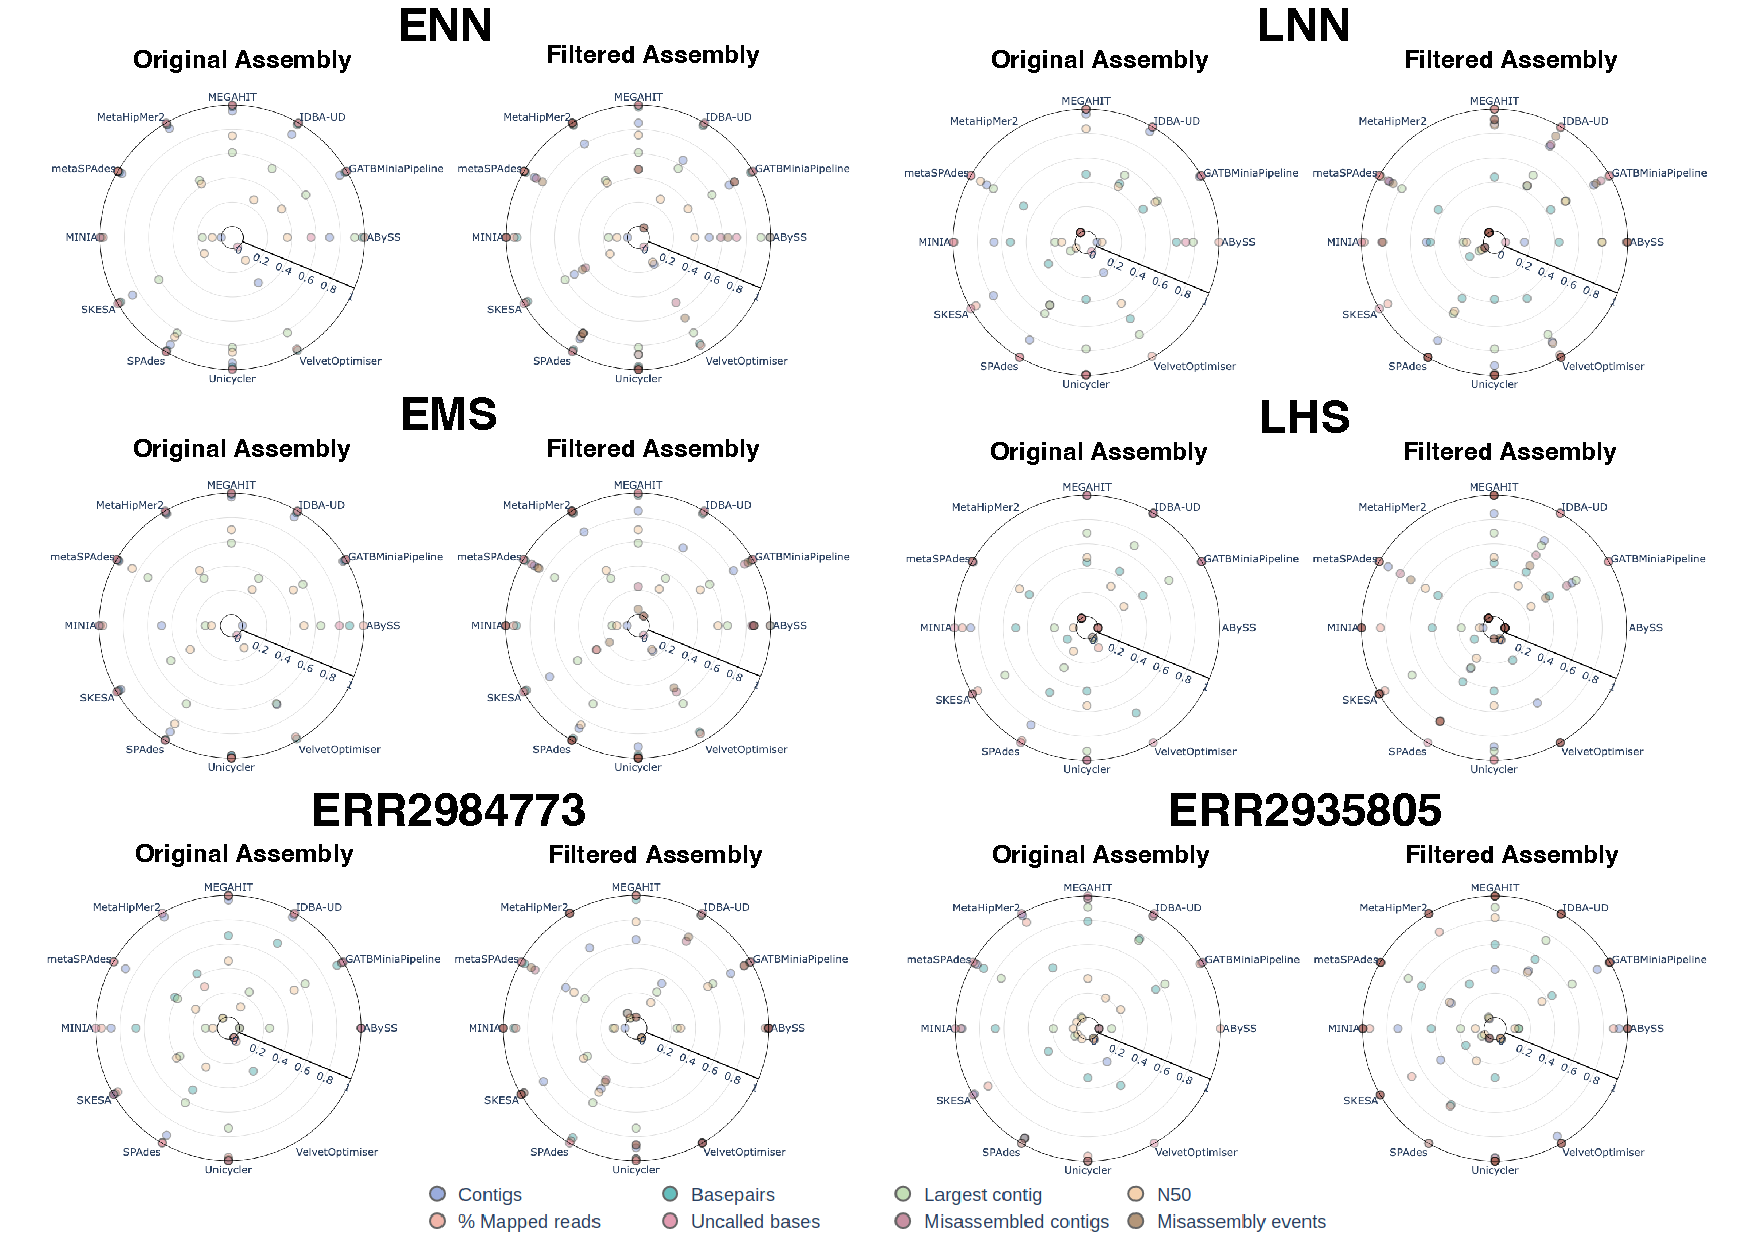
\includegraphics[width=\textwidth]{figures/chapter 5/Figure 4.pdf}
\caption{Assembler performance for the ZymoBIOMICS Microbial Community Standards dataset. For each sample in the dataset, the best score of each assembler in the 3 LMAS runs was selected. The results for each global assembly metric was normalised, with 1 representing the best result, and 0 the worst. For the original assembly, the following metrics are presented: number of contigs produced (in blue), number of basepairs produced (in teal), the size of the largest contig assembled (in green), N50 (in yellow), percentage of mapped reads to the assembly (in orange) and uncalled bases (in red).  For the filtered assembly, the additional metrics are presented: number of misassembled contigs (in purple) and number of misassembly events (in brown). }
\label{fig:chap5_figure4}
\end{figure*}

\subsection{Metagenomic dedicated assemblers do not outperform genomic assemblers}

After excluding the poorly performing assemblers, LMAS includes 3 genomic (SKESA, SPAdes and Unicycler) and 4 labelled as metagenomic specific (GATBMiniaPipeline, IDBA-UD, MEGAHIT and metaSPAdes) de novo prokaryotic assemblers, all implementing multiple k-mer \ac{dBg} algorithms. As observed in Figure \ref{fig:chap5_figure5}, Supplementary Table \ref{tab:ch5_suptable13} and Supplemental Figure \ref{fig:chap5_sup_figure_3},  there were very significant differences between the best and the worst performing assemblers of each type for the ZymoBIOMICS Microbial Community Standards dataset, with this difference being more pronounced for metagenomic assemblers. The best performing assemblers of each type behaved frequently quite similarly, and the differences between them tended to be attenuated after filtering for contigs <1 k\ac{bp}. Still, for the linearly distributed samples (ENN, EMS and ERR2984773), the overall worst performers tended to be metagenomic assemblers. In contrast, for the logarithmically distributed samples (LNN, LHS and ERR2935805) the opposite was observed, with genomic assemblers tending to be the worst-performing (Figure \ref{fig:chap5_figure5}). For the logarithmically distributed samples, the number of basepairs recovered is significantly lower than expected from their composition for both genomic and metagenomic assemblers, particularly after filtering (Supplementary Table \ref{tab:ch5_suptable13}), as contigs representing the less abundant species are not recovered by either type of assemblers (see Assembler performance is influenced by replicon abundance in the sample). For this dataset, the fact that an assembler is branded as genomic or metagenomic does not translate into better or worse performance in dealing with these complex samples, but rather characteristics of the individual assemblers themselves determine their performance.

\begin{figure*}[h!]
\centering
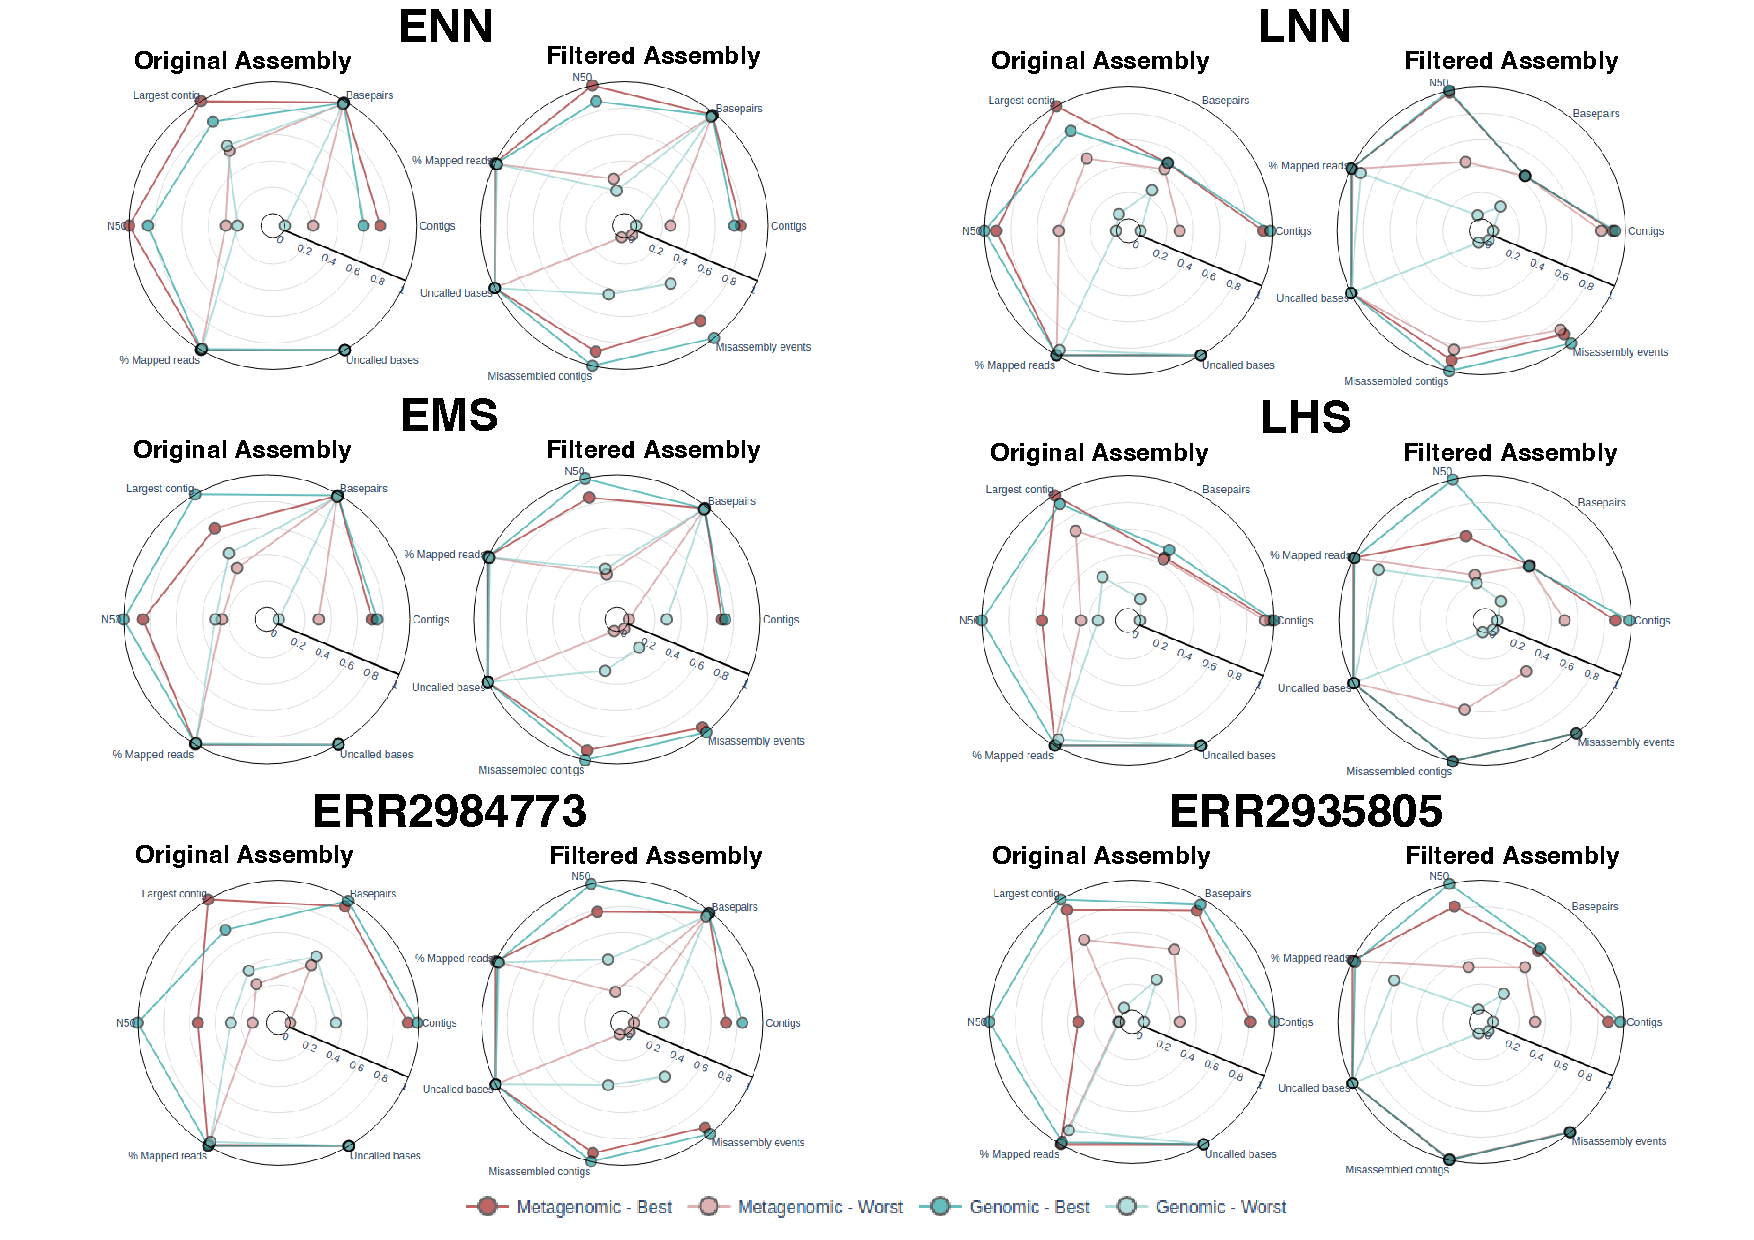
\includegraphics[width=\textwidth]{figures/chapter 5/Figure 5.pdf}
\caption{Performance of genomic and metagenomic assemblers for the ZymoBIOMICS Microbial Community Standards dataset. For each sample in the dataset and for the 3 runs, the best and worst scores for each assembler category were selected: genomic (in blue) and metagenomic (in red). The results for each global assembly metric were normalised, with 1 representing the best result, and 0 the worst. For the original assembly, the following metrics are presented: number of contigs produced, number of basepairs produced, the size of the largest contig assembled, N50, percentage of mapped reads to the assembly and uncalled bases.  For the filtered assembly, the additional metrics are presented: number of misassembled contigs and number of misassembly events.}
\label{fig:chap5_figure5}
\end{figure*}

In the BMock standard, similarly to the ZymoBIOMICS standard, no significant difference was observed between the genomic and metagenomic assemblers, particularly after filtering for contigs <1 kbp (Supplemental Table \ref{tab:ch5_suptable26}). Both \textit{Marinobacter} replicons (2615840697 and 2616644829; 448x and 135x coverage, respectively) were successfully recovered by all genomic and metagenomic assemblers with >0.87 breadth of coverage (Supplementary Table \ref{tab:ch5_suptable27}). The two most abundant \textit{Micromonospora} replicons (2623620557 and 2623620567; 15x and 18x coverage, respectively) were also recovered to a breadth of coverage >0.95 by most assemblers, except the genomic assemblers SKESA and Unicycler (Supplementary Table \ref{tab:ch5_suptable27}). All assemblers, with the exception of SKESA and GATBMiniaPipeline, recovered both Halomonas replicons (2623620617 and 2623620618) with a breadth of coverage of >0.84 (Supplementary Table \ref{tab:ch5_suptable27}). When considering this set of closely related replicons metagenomic assemblers also did not perform consistently better than genomic assemblers in the number of misassembled contigs or SNPs relative to the reference genome. Among the metagenomic assemblers, GATBMiniaPipeline and IDBA-UD performed particularly well but with values close to those of the two best genomic assemblers (SPAdes and Unicycler). IDBA-UB performed significantly worse with the \textit{Micromonospora} replicons, possibly because of their lower coverage. As could have been expected, the number of SNPs in the lower coverage \textit{Halomonas} replicon was consistently higher than in the one with higher coverage (1.6-fold to 85.0-fold depending on the assembler), despite their relatively modest (12.6\%) difference in estimated coverage in the sample and very significant depth of coverage (>500x) (Supplementary Tables \ref{tab:ch5_suptable24} and \ref{tab:ch5_suptable27}). However, when comparing the number of SNPs in the \textit{Marinobacter} replicons, this relationship is reversed, with the replicon with higher coverage (448x) having more SNPs relative to the reference than the one with lower coverage (135x) (Supplementary Table \ref{tab:ch5_suptable27}). This indicates that other factors, such as characteristics of the replicon, the actual representation in the sample and the closeness to other replicons in the sample may influence the performance of assemblers. It is also interesting to see that the contigs generated by themselves do not allow the distinction of closely related strains, since the number of SNPs relative to the reference genomes (if the assembler is able to cover >0.79 of the genome), are in the ranges of 315-9,915 and 9,773-70,196 for the higher and lower depth of coverage \textit{Halomonas} replicons, respectively. 

For the Gut-Mix-RR and Gut-HiLo-RR mock communities, the same pattern was observed as with the other mock communities, with the differences between the metagenomic and genomic assemblers being attenuated after filtering for contigs <1 kbp (Supplemental Table \ref{tab:ch5_suptable30} and \ref{tab:ch5_suptable31}). Particularly for the evenly distributed Gut-Mix-RR sample, when considering the subset of \textit{Roseburia} spp., the replicon with the lowest coverage (12x for \textit{R. intestinalis} versus 18x for \textit{R. hominis}) had a consistently higher number of SNPs, with the exception of the SKESA assemblies, where the opposite was observed. This is similar to what was observed for the \textit{Halomonas} replicons in the BMock12 community standard.

\subsection{Success is not straightforward}

Several factors contribute to suboptimal performance of the assembly process, from DNA isolation and library preparation protocol; sequencing technology, depth and read length; to possible contamination and inherent characteristics of the sample composition.

\subsubsection{Assembler performance is influenced by species}

For the eight bacterial genomes present in the ZymoBIOMICS Microbial Community Standards dataset samples, even in those with an even distribution of the genomes (ENN, EMS and ERR2984773), variations in the assembly metrics were observed (Figure \ref{fig:chap5_figure6}, Supplemental Figures \ref{fig:chap5_sup_figure_4}-\ref{fig:chap5_sup_figure_6}, Supplemental Tables \ref{tab:ch5_suptable14}-\ref{tab:ch5_suptable16}).  For all samples in the dataset, the genomes are recovered almost completely, with all replicons being >90\% represented in the resulting assemblies. \textit{Lactobacillus fermentum} is the least represented genome (92.2\%-94.9\%). Most replicon sequences are recovered in <100 contigs, except for \textit{Pseudomonas aeruginosa}, \textit{Escherichia coli} and \textit{Salmonella enterica}, and not considering IDBA-UB, which frequently produces a larger number of contigs when compared to other assemblers. However, in other mock samples these worse performance of IDBA-UD in terms of number of contigs is not so clear. The absolute values of other metrics of assembly quality, such as \ac{LSA}, misassembly events or uncalled bases, are also different between bacterial genomes (Supplemental Tables \ref{tab:ch5_suptable14}-\ref{tab:ch5_suptable16}). The fact that \textit{S. enterica} is a closely related species to \textit{E. coli}, with high level of genetic similarity (ANIb >0.8, Supplemental Table \ref{tab:ch5_suptable23}), could have created difficulties for resolving the assemblies in a mixed sample and lead to the lower coverage observed, the higher number of contigs and the increased number of misassembled contigs identified in these species in some samples. However, in the case of the larger number of contigs of \textit{P. aeruginosa}, no related species are present in the sample and these possibly reflect intrinsic properties of the replicon such as a high number of prophages integrated in the bacterial genome \cite{johnson_complete_2019}. Similarly, replicon characteristics could be behind the lower breadth of coverage consistently observed in \textit{L. fermentum} assemblies. 

\begin{figure*}[h!]
\centering
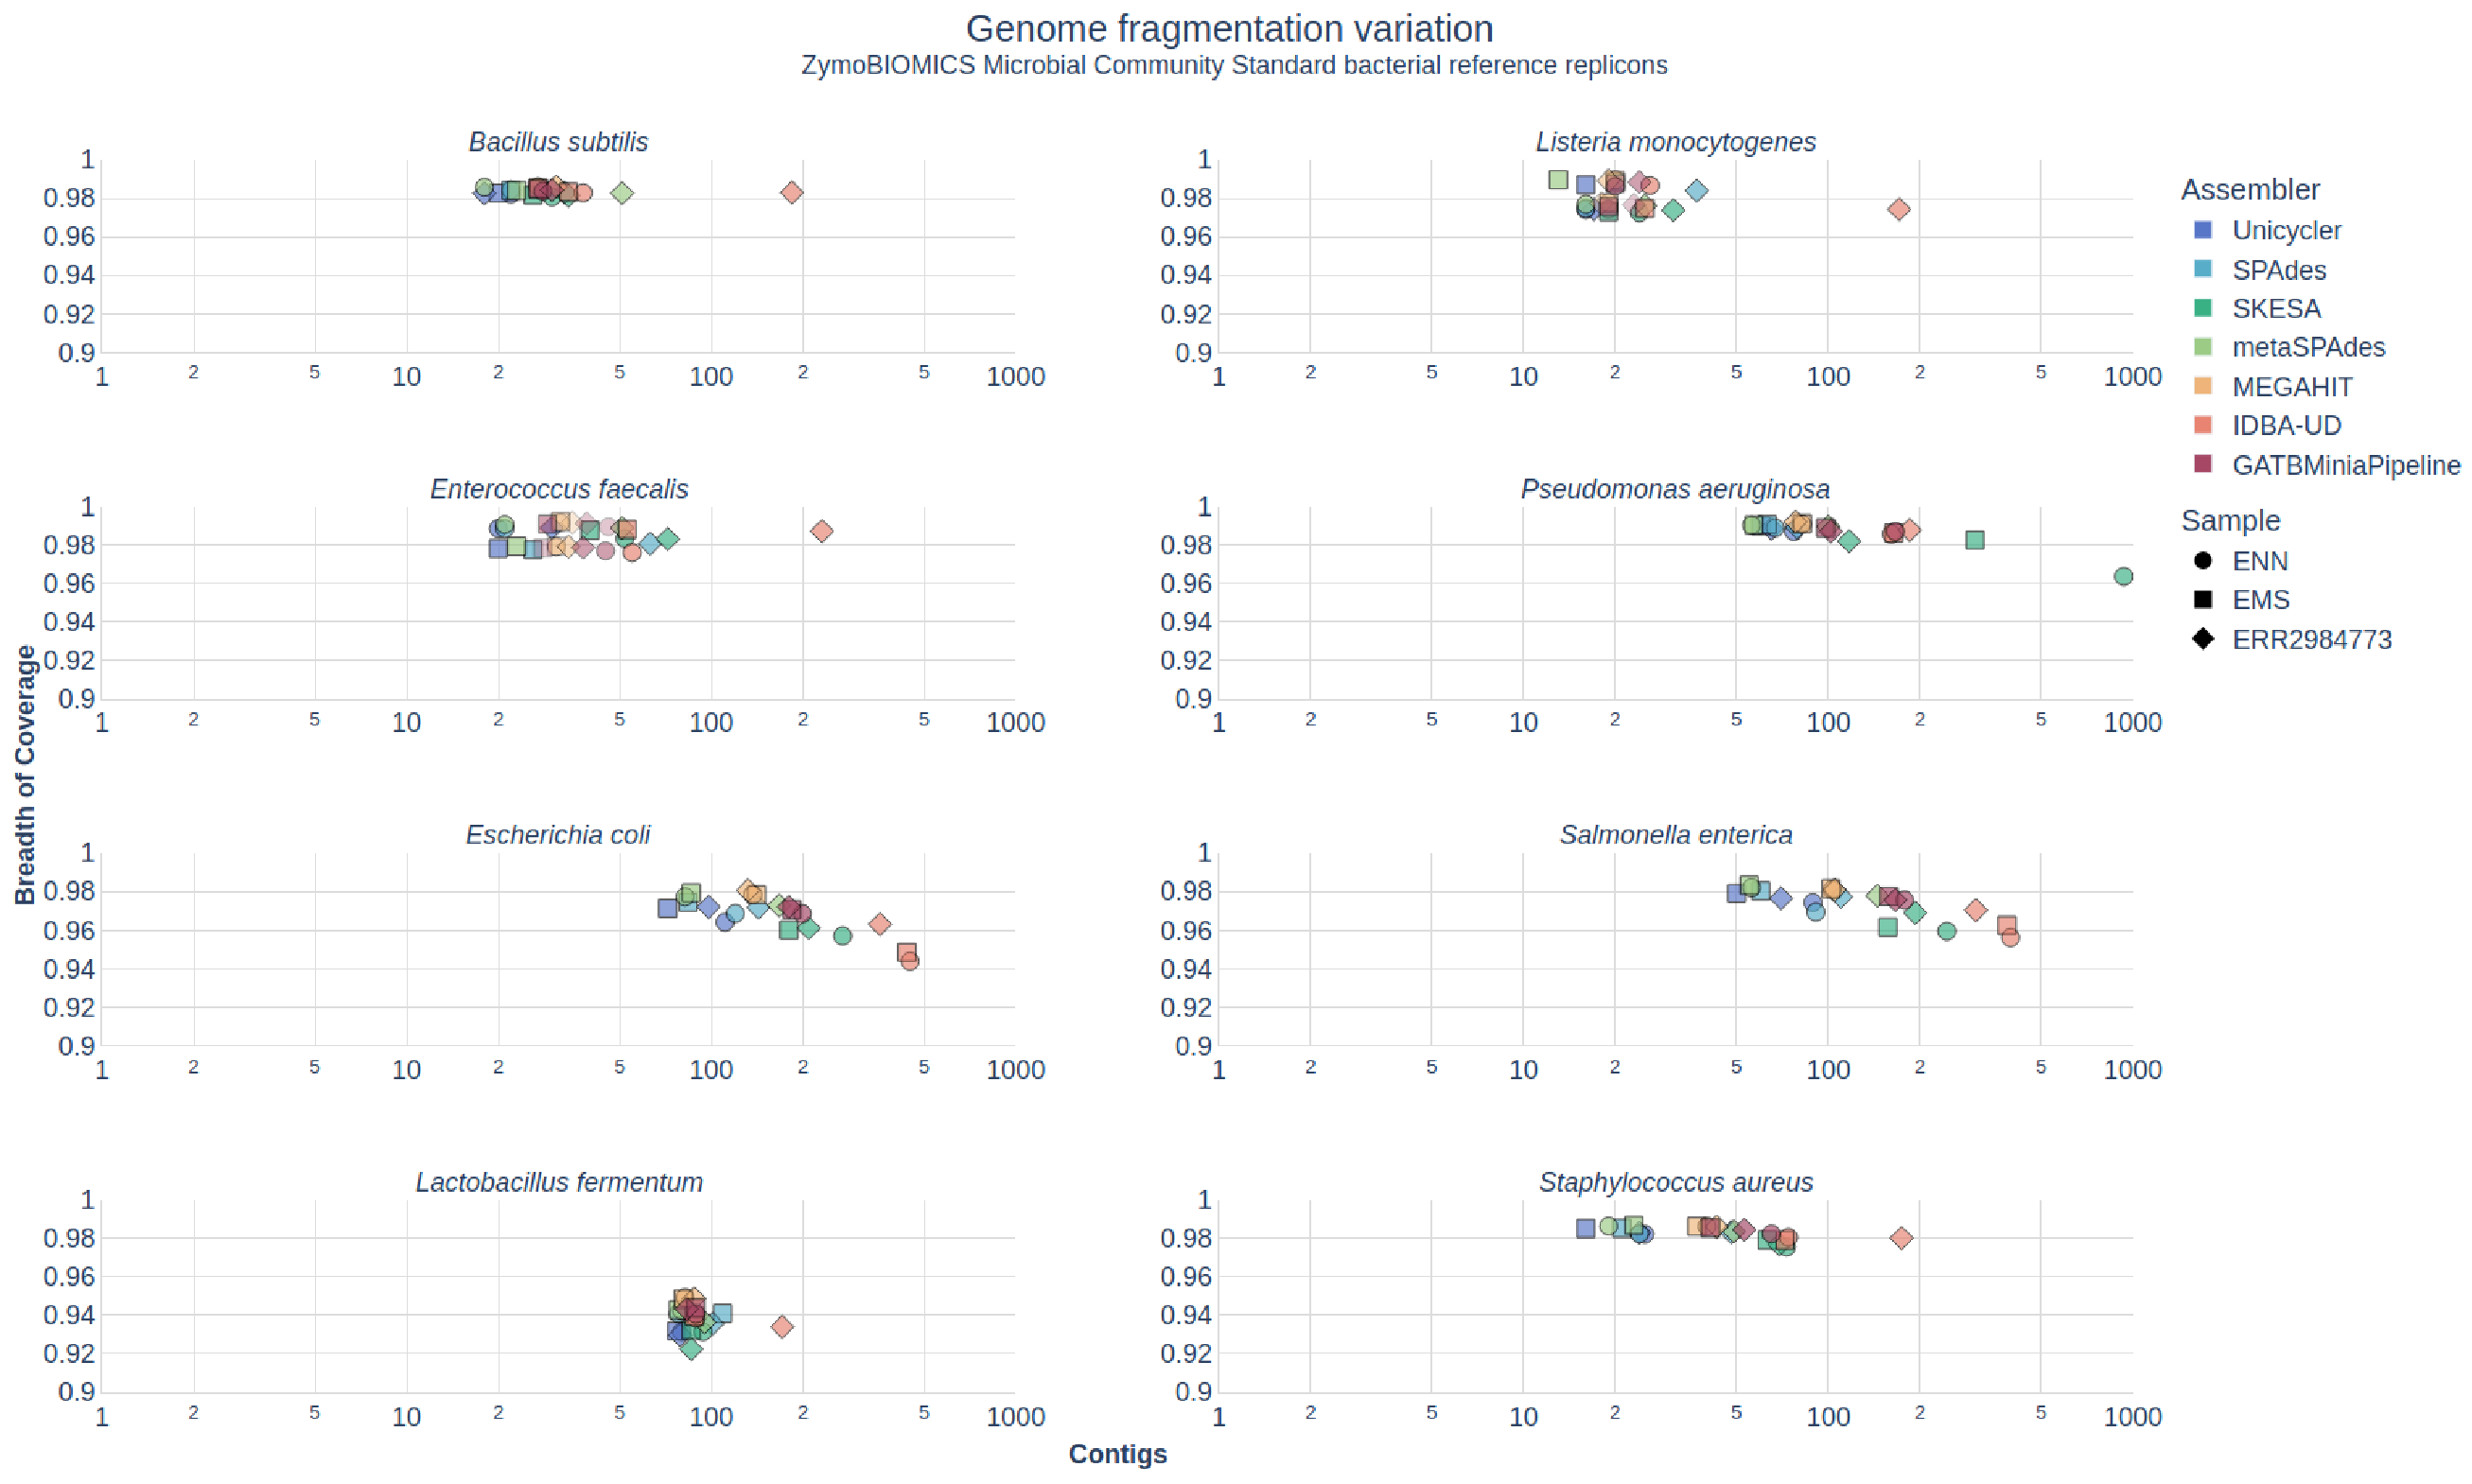
\includegraphics[width=\textwidth]{figures/chapter 5/Figure 6.pdf}
\caption{Genome fragmentation for each reference replicon of the ZimoBIOMICS community standards dataset for the evenly distributed samples. Genome fragmentation for the 3 LMAS runs is represented by the number of contigs and breadth of coverage of the reference per assembler for the evenly distributed samples: ENN (evenly distributed without error model, identified by a circle), EMS (evenly distributed with Illumina MiSeq error model, identified by a square) and ERR2984773 (real Illumina MiSeq sample, identified by a diamond). Each assembler is identified with the following colour scheme - dark blue: Unicycler, light blue: SPAdes, dark green: SKESA, light green: metaSPAdes, yellow: MEGAHIT, orange: IDBA-UD, red: GATBMiniaPipeline.}
\label{fig:chap5_figure6}
\end{figure*}

In the BMock12 and the Gut-Mix samples, which have pairs of much more similar replicons, it is true that the closely related replicons do have higher numbers of contigs. However, it is possible that the properties of the individual replicons also have an impact on the number of contigs generated by the assemblers (Supplemental Figure S8). Another potential confounder which was not explored is the length of the reads, with Miseq samples having 300bp reads and HiSeq samples having 150bp reads.

\subsubsection{Longer contigs have higher confidence}

The \ac{Pls} metric, which measures the error rate of a contig relative to the reference, shows that for every replicon, longer contigs have higher \ac{Pls} (Figure \ref{fig:chap5_figure7}). This could justify the option of filtering an assembly by length, even beyond the 1000 \ac{bp} minimum contig size implemented by default in LMAS. Not only are we eliminating shorter, less informative contigs in terms of genetic context, but these are also the ones most likely to contain errors relative to the reference sequence. 

\begin{figure*}[h!]
\centering
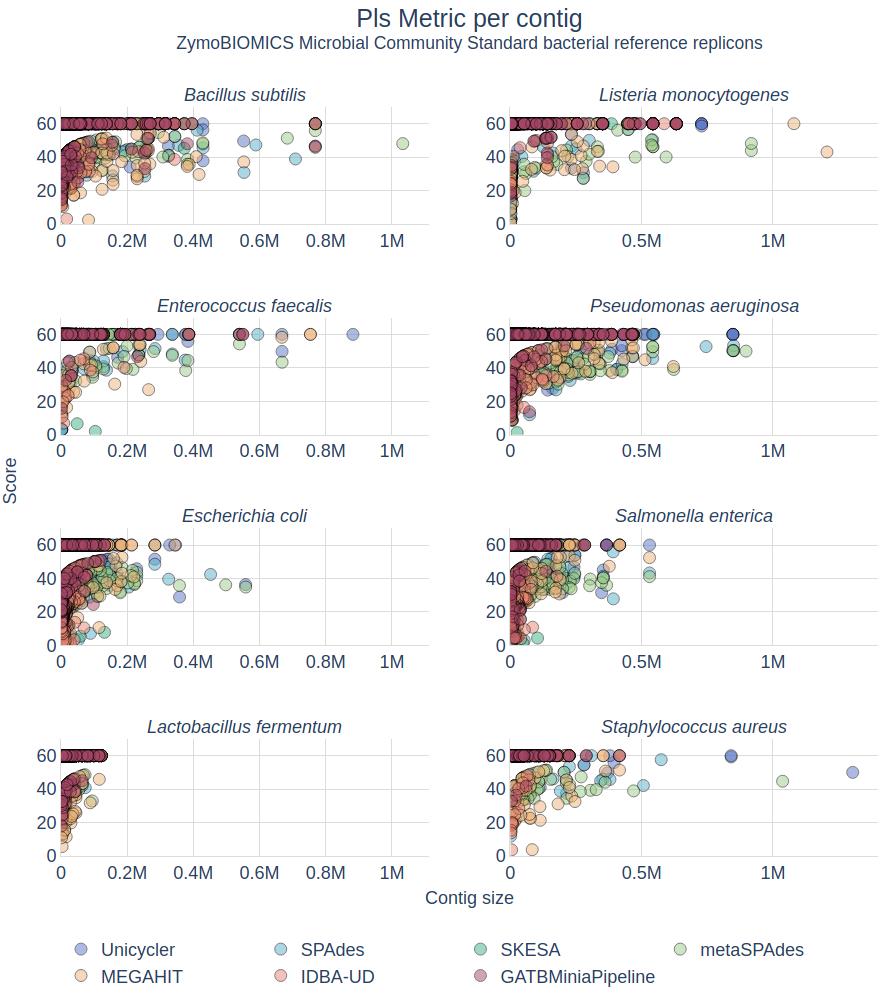
\includegraphics[width=\textwidth]{figures/chapter 5/Figure 7.png}
\caption{: Phred-like score (\ac{Pls}) per contig for each reference replicon of the ZimoBIOMICS community standards datasets. The \ac{Pls} score was calculated for each unique contig produced by each assembler in 3 LMAS runs and is represented in relation to its contig size. Each contig is coloured according to the assembler with the following colour scheme - dark blue: Unicycler,  light blue: SPAdes, dark green: SKESA, light green: metaSPAdes, yellow: MEGAHIT, orange: IDBA-UD, red: GATBMiniaPipeline.}
\label{fig:chap5_figure7}
\end{figure*}

\subsubsection{Longer contigs have higher confidence}

Some genomic regions in several replicons are consistently a challenge for all assemblers. As observed in Figure \ref{fig:chap5_figure8}, all genomes of the ZymoBIOMICS Microbial Community Standards dataset present certain regions that fail to assemble for all tools in all runs, even those generating high-quality draft assemblies. Of all seven assemblers considered, only GATBMiniaPipeline, MEGAHIT and IDBA-UD showed inconsistency in the gaps produced over the 3 LMAS runs (Supplemental Table \ref{tab:ch5_suptable17}), as expected from producing variable sets of contigs. The regions consistently missing for all assemblers in all runs are rich in repetitive elements, such as rRNA and tRNA coding sequences and mobile genetic elements (Supplemental Table \ref{tab:ch5_suptable18}), with larger gaps corresponding to tandem sets of these elements. This reflects an intrinsic limitation of short-read sequencing since the length of a read pair is not enough to bridge across the repetitive element, preventing the generation of contigs representing these regions. This is something that could be addressed by the use of long-read sequencing technologies. Despite this, some assemblers are able to produce contigs that represent some of these large tandem regions, such as MEGAHIT and SKESA for \textit{E. faecalis}, and IDBA-UD, MEGAHIT and metaSPADES for \textit{L. monocytogenes}, but such performance is not consistent for all reference replicons. For instance, SKESA fails to assemble two large regions of the \textit{S. enterica} genome that all other assemblers successfully cover.

\begin{figure*}[h!]
\centering
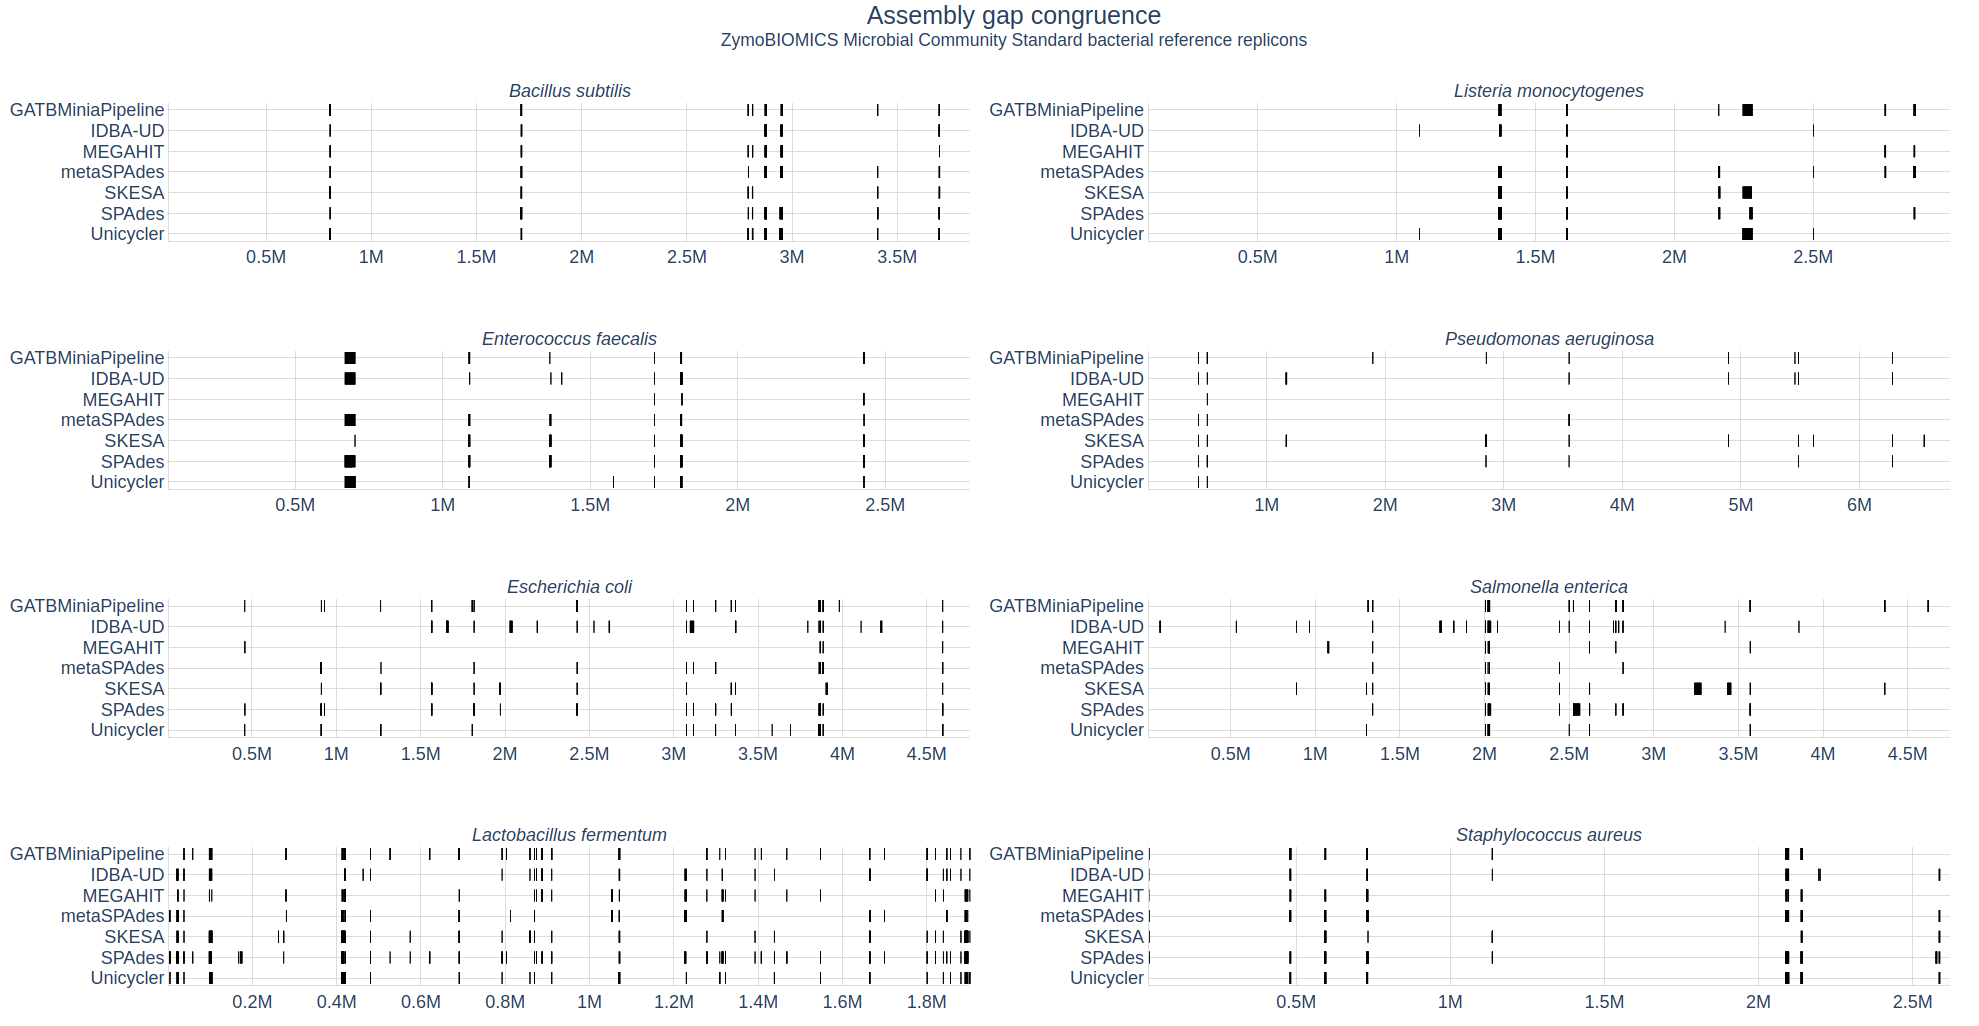
\includegraphics[width=\textwidth]{figures/chapter 5/Figure 8.png}
\caption{Location of gaps in comparison to the reference sequence, per assembler, for each reference replicon of the ZimoBIOMICS community standards datasets. The resulting plot contains the consistent gaps obtained from a three LMAS run for the evenly distributed dataset (ENN, EMS and ERR2984773) for GATBMiniaPipeline, IDBA-UD, MEGAHIT, metaSPAdes, SKESA, SPAdes and Unicycler assemblers.}
\label{fig:chap5_figure8}
\end{figure*}

For the BMock12 community standard, the same pattern of consistency of difficult regions across replicons can be observed for all replicons, with the exception of the lowest abundance replicons (see Supplemental Figure S9). Interestingly, the two closely related \textit{Halomonas} replicons present a very dissimilar gap pattern, and with a high number of gaps (n=2789 and n=2702) distributed throughout the replicon sequence, which possibly reflects the difficulty of assembling closely related replicons in the same sample.

\subsubsection{Assembler performance is influenced by replicon abundance in the sample}

The logarithmically distributed samples (LNN, LHS and ERR2935805) of the ZymoBIOMICS community standard dataset showed greater variation in the assembly success metrics than the evenly distributed samples (Supplementary Table \ref{tab:ch5_suptable8}-\ref{tab:ch5_suptable10}), reflecting the difficulty of recovering sequences of the lowest abundant replicons. For the three replicons with an estimated depth of coverage >15x, a similar pattern is observed in logarithmically distributed samples as in evenly distributed samples, albeit with greater dispersion in the number of contigs generated and with a markedly decreased breath of coverage for some assemblers and samples in the logarithmically distributed samples (Figure \ref{fig:chap5_figure6} and Supplementary Figure \ref{fig:chap5_sup_figure_7}). Almost no contigs >1000 \ac{bp} were retrieved for replicons with an estimated depth of coverage of <2x resulting in a very low breadth of coverage (<1\%) (Supplementary Table \ref{tab:ch5_suptable4}, Supplementary Table \ref{tab:ch5_suptable22}). This leads to a severe underrepresentation of the diversity of the community in the generated contigs, particularly of plasmid sequences due to their smaller length and abundance as was described previously \cite{sczyrba_critical_2017,meyer_critical_2022, fritz_camisim_2019}. This happens despite the greater sequencing depth of these samples versus those with an even distribution (>5-fold difference in the number of reads).

For the BMock12 community standard, the very low replicon abundance (\textit{Micromonospora coxensis}, 2623620609, 0.02x coverage), fails to assemble in all tools (Supplemental Figure S9, Supplemental table S24). The \textit{Micromonospora echinaurantiaca} (2623620557, 14.9x coverage) and \textit{Micromonospora echinofusca} (2623620567, 18.2x coverage) fail to assemble with SKESA and Unicycler, and the \textit{Propionibacteriaceae} replicon (2615840646, 31.9x coverage) fails to be assembled with SKESA. In the Gut-Mix-RR standards there are several replicons with <1x to 20x depth of coverage. Significant breath of coverage (>0.7) was obtained with the contigs created by most assemblers, including successful assemblies of some of the replicons by SKESA and Unicycler that had failed with higher coverage replicons in the BMock12 standard. Taking together these data and that of the ZymoBIOMICS standard, these suggest that it is hard to establish a universal breakpoint at which each of the assemblers is able to generate high breadth of coverage contigs, with the actual genome of interest and the composition of the sample possibly playing a role. Nevertheless, coverages >15x result in high breadth of coverage contigs, albeit in the lower range with many contigs and a significant number of SNPs.

\section{Conclusions}

The purpose of LMAS is to empower users to test assembler performance in meaningful conditions for their experimental setup and objectives. Suitable mock communities, reproducing the users’ samples of interest, can be used as a gold standard to evaluate assembler performance. To illustrate LMAS’ functionalities we analysed three well-known samples used in several studies. Although the eight species ZymoBIOMICS Microbial Community Standards might not be representative of the metagenomic complexity of the samples of interest of most researchers,we hoped that its relative simplicity meant that the results shown would represent a best-case scenario, since as sample complexity increases so do the challenges to assembler performance. However, the results of the BMock12 and Gut-Mix community standards suggest that the actual genome of interest and community composition play an important part in the results of individual assemblers. 

Our results showed significant differences in both global and reference-dependent assembly quality metrics generated by each de novo assembler. The performance of each assembler varied depending on the species of interest and its abundance in the sample, with less abundant species presenting a significant challenge for all assemblers. The fact that an assembler is branded as specific for metagenomics does not guarantee a better performance in metagenomic samples, with assemblers used for genomic assembly outperforming the worst metagenomic assembler tested. Even when considering communities with very similar replicons, the overall performance of metagenomic assemblers was not consistently better than that of genomic assemblers. The results also indicate that the recovery of assemblies allowing strain-level discrimination at the SNP level is highly unlikely based solely on the assembler generated contigs. The following assemblers showed significant performance problems and their usability may be limited, at least with the default parameters we used: ABySS, MetaHipmer2, minia and VelvetOptimiser.

The choice of de novo assembler depends greatly on the computational resources available, the species of interest, its representation in the sample, and, possibly, the composition of the community in the sample. In our testing with any of the mock communities, no assembler stood out as an undisputed all-purpose choice for short-read metagenomic prokaryotic genome assembly, with different assemblers showing specific strengths. Users would thus benefit from analysing the results of sequencing mock communities (ideally) or of artificially generated reads simulating their samples of interest to guide their choice of assembler. LMAS was developed to be an easy to use and flexible tool for this purpose. From the results that we obtained with various mock communities, the following assemblers performed consistently well (presented in alphabetical order): MEGAHIT, metaSPAdes, SKESA, SPAdes and Unicycler. From our assessment, we conclude that these assemblers are the most likely candidates to perform well in other complex samples.

LMAS was built with modularity and containerization as keystones, leveraging the parallelization of processes and guaranteeing reproducibility across platforms. The modular design allows for new assemblers to be easily added and existing assemblers to be easily updated, allowing LMAS to function as a continuous benchmarking platform and ensuring its future relevance as improvements in assembly software are proposed. LMAS will also support evaluating the gains of any cumulative improvements to existing assemblers  using the same benchmark set adapted to a specific project or goal. Such reproducibility, capacity to easily add assemblers of interest not included in the current version and flexibility for future extensions are important principles in computational method benchmarking. Moreover, users may compare software performance against mock communities of special interest, depending on their operational focus. Moreover, by lowering the barriers to perform comparisons between assemblers, LMAS will encourage users may compare software performance against mock communities of special interest, depending on their operational focus.

The interactive report provides an intuitive platform for data exploration, allowing the user to easily sift through global and reference specific performance metrics for each sample, as well as providing information on the assemblers executed to allow traceability of the results. Producing an extensive, metric rich report allows users interested in different aspects of assembler performance to make informed decisions, particularly when choosing among the top-performing assemblers, which show only minor differences.

LMAS applies several well-known assembly metrics and proposes two more: \ac{LSA}, which represents the fraction of the longest single alignment between a contig and the reference, and \ac{Pls}, a scoring function based on the identity of each aligned contig to the reference replicon. The entire set of assembly quality metrics used in LMAS allows not only the assessment of quality based on statistics inherent to a set of assembled contigs but also a comparison to a ground truth provided through the use of samples of known composition and reference sequences. The LMAS report provides an interactive and intuitive platform for the exploration of these results, allowing users to easily test assemblers in mock samples with species composition and distribution relevant for their own studies.

Although computationally intensive due to the complex nature of the de novo assembly process, LMAS is the only software integrating assembly and its evaluation into a single pipeline, guaranteeing the same conditions are met for all tools. With LMAS, it is now possible to evaluate which de novo assembler produces the most relevant results for a given community of interest. The LMAS workflow is open-source and its code and documentation are available at \url{https://github.com/B-UMMI/LMAS} and \url{https://lmas.readthedocs.io/} respectively.

\section{Availability of supporting source code and requirements}

\textbf{Project name:} LMAS

\textbf{Project home page: }https://github.com/B-UMMI/LMAS 

\textbf{Operating system(s):} UNIX-like systems.
Programming languages: Nextflow, Python, Bash, Javascript

\textbf{Other requirements: }Java version 8 or highest. Docker/Singularity/Shifter

\textbf{License: } GNU GPL v3

\textbf{RRID:} SCR\_022251


\section{Declarations}

\subsection{Ethics approval and consent to participate}

Not applicable.

\subsection{Consent for publication}

Not applicable.

\subsection{Availability of data and material}

The datasets analysed during the current study are available in the Zenodo repository, under \url{https://doi.org/10.5281/zenodo.4588969}. All supplemental material is available in the Zenodo repository, under \url{https://doi.org/10.5281/zenodo.6623457}. Likewise, all figures in the current manuscript are available in their original format in the Zenodo repository, under \url{https://doi.org/10.5281/zenodo.6783042}. Real sequencing data of the ZymoBIOMICS Microbial Community Standards is available under accessions ERR2984773 and ERR2935805 \cite{nicholls_ultra-deep_2019}. All data generated or analysed during this study are included in this published article, its supplementary information files and the data analysis repository located at \cite{noauthor_lmas_2022}. Additionally, the reports for the ZymoBIOMICS Microbial Community Standard, BMock12 Community Standard and NIBSC Gut DNA Reference are available at \url{https://doi.org/10.5281/zenodo.7088960}, \url{https://doi.org/10.5281/zenodo.7092431} and \url{https://doi.org/10.5281/zenodo.7092693} respectively.

\subsection{Competing interests}

MR received honoraria for serving on the speakers' bureau of Pfizer and Merck Sharp and Dohme and for participating in expert panels of GlaxoSmithKline and Merck Sharp and Dohme. The other authors declare that they have no competing interests.  

\subsection{Funding}

C.I.M. was supported by the Fundação para a Ciência e Tecnologia (grant SFRH/BD/129483/2017).

\subsection{Author’s contributions}

C.I.M., M.R. designed the workflow. C.I.M implemented and optimised the workflow, created the Docker containers, generated mock shotgun metagenomics data used to test and validate the workflow, contributed to the development of the HTML report and analysed the data. C.I.M. and M.R. wrote the manuscript. P.V.C. contributed to the development of the HTML report. M.R., J.A.C. Y.M, and J.M.G critically revised the manuscript.  All authors read, commented on, and approved the final manuscript. 

\subsection{Acknowledgements}

The authors would like to thank Rafael Mamede for his contribution to the implementation and commentary on the several interactive plots implemented throughout the LMAS report. The authors would also like to thank Nabil Fareed-Alikan for his insightful commentary on the interpretation of the results reported in this manuscript, and Anthony Underwood and Robert A. Petit III for their assistance in building the LMAS Nextflow workflow. The author would also like to thank Samuel Nicholls, Joshua Quick, Shuiquan Tang and Nicholas Loman for publicly providing the sequencing data for the ZymoBIOMICS Microbial Community Standards. Likewise, the authors would like to thank Volkan Sevim, Juna Lee, Robert Egan, Alicia Clum, Hope Hundley, Janey Lee, R. Craig Everroad, Angela M. Detweiler, Brad M. Bebout, Jennifer Pett-Ridge, Markus Göker, Alison E. Murray, Stephen R. Lindemann, Hans-Peter Klenk, Ronan O’Malley, Matthew Zane, Jan-Fang Cheng, Alex Copeland, Christopher Daum, Esther Singer & Tanja Woyke for providing the sequencing data for the BMock12 Commynity Standard, and to Gregory C. A. Amos, Alastair Logan, Saba Anwar, Martin Fritzsche, Ryan Mate, Thomas Bleazard & Sjoerd Rijpkema for providing the sequencing data of the NIBSC Gut DNA Reference Gut-Mix-RR and Gut-Mix-HiLo Community Standard.

\section{Supplemental Materials}

\subsection{Workflow parameters}

In LMAS, a set of default parameters is provided but these can be altered, either by passing the new value when executing the workflow or by editing the “params.config” file in the “configs” folder. There are three main parameters in LMAS: “reference”, “fastq” and “md”. The short-read data is passed as input through the “--fastq” parameter, which by default is set to match all files in the “data/fastq” folder that match the pattern “*\_R{1,2}*”. The reference sequences in a single file can be passed with the “--reference” parameter, matching by default fasta files (with the pattern “*.fasta”) in the “data/reference” folder. Although not mandatory, text information, in a markdown file, on input samples can be passed to LMAS to be presented in the report with the “--md” parameter. By default, this is matched to the “*.md” pattern in the “data” folder.  

Several options are available to alter the behaviour of the assemblers incorporated in LMAS, namely to alter the values of the k-mer for each assembly iteration, as detailed in the documentation \cite{}. By default, these values reflect the corresponding default settings of the assemblers. Additionally, each assembler can be skipped from the workflow, and the resources for the execution, such as CPUs, memory and time limit, can be altered for all assembly processes. For the assembly quality assessment performed by LMAS, the following parameters are provided and can be adjusted: 

\begin{itemize}
    \item \textbf{ “--minLength”:} Value for minimum contig length, in basepairs. By default, this value is set to 1000 basepairs;
    \item \textbf{“--mapped\_reads\_threshold”:} Value for the minimum percentage of a read aligning to the contig to be considered as mapped. By default, this value is set to 75\%;
    \item \textbf{“--n\_target”:} Target value for the N, NA and NG metrics, ranging from 0 to 100\%. By default, this value is set to 50\%;
    \item \textbf{“--l\_target”:} Target value for the L metric, ranging from 0 to 100\%. By default, this value is set to 90\%;
\end{itemize}

\subsection{Short-read de novo assemblers} \label{ch5_sup_assemblers}

We have compiled a collection of de novo assembly tools, including \ac{OLC} and \ac{dBg} assembly algorithms, with both single k-mer and multiple k-mer value approaches, and hybrid assemblers (Supplemental Table \ref{tab:ch5_suptable1}). The collection includes both genomic and metagenomic assemblers, developed explicitly to handle metagenomic datasets. The dates of the last release correspond to the ones available in the preparation of this manuscript.

\subsubsection{Selection Criteria}

Only open-source tools, with clear documentation describing the methodology implemented, were considered. The collection of tools was ordered by the date of the last update, and a Docker container \cite{noauthor_docker_nodate} for the top 11 assemblers was created with the latest released version, with the version used as the tag. In the case of tools where a versioned release is not available, the container was created with the latest version in the default branch of the source repository, using the date of the last update as the tag. The PANDAseq \cite{masella_pandaseq_2012} assembler was excluded due to execution errors. 

\subsubsection{Assemblers in LMAS}

Assemblers benchmarked in LMAS, in alphabetical order:

\paragraph{ABySS} \mbox{}\\

The ABySS assembler \cite{jackman_abyss_2017} is a de novo sequence assembler intended for short paired-end reads and genomes of all sizes. It follows the model of minia, wherein a probabilistic Bloom filter representation is used to encode the de single k-mer size Bruijn graph, reducing memory requirements for de novo assembly. The code is open-source and available at \cite{noauthor_abyss_2022}. The following command is used: “abyss-pe name='\$sample\_id'k=\$KmerSize B=\$BloomSize in='\$fastq”, where “\$sample\_id” contains the identifier of the sample,  contains a list of the input read files, “\$sample\_id” the identifier of the sample, “\$KmerSize” the length of the nodes of the graph (by default set to 96), “\$BloomSize” the size, in Gb, of the bloom filter (by default set to 2 GB), and “\$fastq” the forward and reverse fastq files. 

\paragraph{GATB-Minia Pipeline} \mbox{}\\

GATB-Minia is an assembly pipeline, still unpublished, that consists of Bloocoo [8] for error correction, minia 3 \cite{chikhi_space-efficient_2013} for contigs assembly, which is based on the BCALM2 assembler \cite{chikhi_compacting_2016}, and BESST \cite{sahlin_besst_2014} for scaffolding. It was developed to extend the minia assembler to use the dBg algorithm with multiple k-mer values and to explicitly handle metagenomic data. The code is open-source and available at \cite{noauthor_gatbgatb-minia-pipeline_2022}. The following command is used: “gatb -1 \$fastq\_pair[0] -2 \$fastq\_pair[1] --kmer-sizes \$kmer\_list -o \$sample\_id”, where \$fastq\_pair[0] contains the forward-facing reads, \$fastq\_pair[1] the reverse-facing reads, \$kmer\_list the list of values for length of the nodes of the dBg (by default set to 21,61,101,141,181), and “\$sample\_id” the identifier of the sample. 

\paragraph{IDBA-UD} \mbox{}\\

IDBA-UD \cite{peng_idba-ud_2012} is a dBg graph assembler for assembling reads from single-cell sequencing or metagenomic sequencing technologies with uneven sequencing depths. It employs multiple depth relative thresholds to remove erroneous k-mers in both low-depth and high-depth regions. The technique of local assembly with paired-end information is used to solve the branch problem of low-depth short repeat regions. To speed up the process, an error correction step is conducted to correct reads of high-depth regions that can be aligned to high confidence contigs. The code is open-source and available at \cite{peng_loneknightpyidba_2022}. The following command is used:  “idba\_ud -l \$fasta\_reads\_single”, where \$fasta\_reads\_single contains the combined sequence data converted to FASTA format reads with “reformat.sh” from BBtools \cite{bushnell_bbmerge_2017}. 

\paragraph{MEGAHIT} \mbox{}\\

MEGAHIT \cite{li_megahit_2015} is a de novo assembler for large and complex metagenomics datasets. It makes use of the succinct dBg, with a multiple k-mer size strategy. In each iteration, MEGAHIT cleans potentially erroneous edges by removing tips, merging bubbles and removing low local coverage edges, especially useful for metagenomics which suffers from non-uniform sequencing depths. The code is open-source and available at \cite{li_megahit_2022}. The following command is used: “megahit -o megahit --k-list \$kmers -1 \$fastq\_pair[0] -2 \$fastq\_pair[1]”, where \$kmers contains the list of values for length of the nodes of the dBg (by default set to 21,29,39,59,79,99,119,141), \$fastq\_pair[0] contains the forward-facing reads, and \$fastq\_pair[1] the reverse-facing reads.

\paragraph{MetaHipMer2} \mbox{}\\

MetaHipMer2 \cite{georganas_extreme_2018} is a  multiple k-mer size dBg de novo metagenome short-read assembler built to run efficiently on both single servers and on multi-node supercomputers, where it can scale up to coassemble terabase-sized metagenomes. The code is open-source and available at \cite{noauthor_berkeleylab_nodate}. The following command is used: “mhm2.py -k \$kmers -r \$fasta\_reads\_single -s 0”, where \$kmers contains the list of values for length of the nodes of the dBg (by default set to “21,33,55,77,99”), where \$fasta\_reads\_single contains the combined sequence data converted to FASTA format reads with “reformat.sh” from BBtools \cite{bushnell_bbmerge_2017}. The “-s 0” option skips the scaffolding step. 

\paragraph{metaSPAdes} \mbox{}\\

SPAdes [19] started as a tool aiming to resolve uneven coverage in single-cell genome data, with metaSPAdes \cite{nurk_metaspades_2017} later released building a specific metagenomic pipeline on top of SPAdes. It uses multiple k-mer sizes of dBg, starting with the lowest kmer size and adding hypothetical k-mers to connect the assembly graph. The code is open-source and available at \cite{noauthor_spades_nodate}. The following command is used: “metaspades.py --only-assembler -k \$kmers -1 \$fastq\_pair[0] -2 \$fastq\_pair[1]”, where \$kmers contains the list of values for length of the nodes of the dBg (by default set to “auto”), \$fastq\_pair[0] contains the forward-facing reads, and \$fastq\_pair[1] the reverse-facing reads.

\paragraph{minia} \mbox{}\\

Minia \cite{chikhi_space-efficient_2013} performs the assembly on a data structure based on unitigs produced by the BCALM \cite{chikhi_compacting_2016} software and using graph simplifications that are heavily inspired by the SPAdes assembler \cite{bankevich_spades_2012}. Minia is a short-read traditional assembler based on dBg graph using a single k-mer length. The code is open-source and available at  \cite{noauthor_minia_2022}. The following command is used: “minia -in \$list\_reads -out \$sample\_id”,  where “\$list\_reads” contains a list of the input read files and “\$sample\_id” the identifier of the sample.

\paragraph{SKESA} \mbox{}\\

SKESA \cite{souvorov_skesa_2018} is a de novo sequence read assembler that is based on dBg and uses conservative heuristics. It is designed to create breaks at repeat regions in the genome, creating shorter assemblies but with greater sequence quality. It tries to obtain good contiguity by using multiple k-mers longer than mate length and up to insert size. The code is open-source and available at \url{https://github.com/ncbi/SKESA}. The following command is used: “skesa --use\_paired\_ends --contigs\_out \$sample\_id --fastq \$fastq\_pair[0] \$fastq\_pair[1]”, where “\$sample\_id” refers to the identifier of the sample, \$fastq\_pair[0] contains the forward-facing reads, and \$fastq\_pair[1] the reverse-facing reads.

\paragraph{SPAdes} \mbox{}\\

SPAdes \cite{bankevich_spades_2012} is an assembly tool aiming to resolve uneven coverage in single-cell genome data through multiple k-mer sizes of dBgs. It starts with the smallest k-mer size and adds hypothetical k-mers to connect the graph. The code is open-source and available at \cite{noauthor_spades_nodate}. The following command is used:  “spades.py --only-assembler -k \$kmers -1 \$fastq\_pair[0] -2 \$fastq\_pair[1] ”, where \$kmers contains the list of values for length of the nodes of the dBg (by default set to “auto”), \$fastq\_pair[0] contains the forward-facing reads, and \$fastq\_pair[1] the reverse-facing reads.

\paragraph{UNICYCLER} \mbox{}\\

Unicycler \cite{wick_unicycler_2017} is an assembly pipeline for bacterial genomes that can do long-read assembly, hybrid assembly and short-read assembly. When assembling Illumina-only read sets, it functions as a SPAdes-optimiser, using a  dBg algorithm with multiple k-mer values. The code is open-source and available at \cite{wick_unicycler_2022}]. The following command is used: “unicycler -o . --no\_correct --no\_pilon -1 \$fastq\_pair[0] -2 \$fastq\_pair[1]”, where \$fastq\_pair[0] contains the forward-facing reads, and \$fastq\_pair[1] the reverse-facing reads.

\paragraph{VELVETOPTIMIZER} \mbox{}\\

This optimising pipeline of the Velvet assembler \cite{zerbino_velvet_2008} is still unpublished but extends the original tool by performing several dBg assemblies with variable k-mer sizes. It searches a supplied hash value range for the optimum, estimates the expected coverage and then searches for the optimum coverage cutoff. It uses Velvet’s internal mechanism for estimating insert lengths for paired-end libraries.  The code is open-source and available at \cite{seemann_velvetoptimiser_2021}. The following command is used: “VelvetOptimiser.pl -v -s \$velvetoptimizer\_hashs -e \$velvetoptimizer\_hashe -f '-shortPaired -fastq.gz -separate \$fastq\_pair[0] \$fastq\_pair[1]'”, where \$velvetoptimizer\_hashs is the lower end of the hash value range that the optimiser will search for the optimum (default: 19), \$velvetoptimizer\_hashe is the upper end of the hash value range that the optimiser will search for the optimum (default: 31), \$fastq\_pair[0] contains the forward-facing reads, and \$fastq\_pair[1] the reverse-facing reads.

\subsection{Misassembly detection} \label{chap5_sup_misassembly}

For the detection of misassembly events in the assemblies, the assembled sequences are first filtered for a minimum sequence length with BBTools \cite{bushnell_bbmerge_2017} (version 38.44), as defined in the parameters, using the following command: “reformat.sh in=\$assembly out=filtered\_\$assembly minlength=\$minLen”, where \$assembly contains the file with the assembled sequences and \$minLen the value of the minimum sequence length allowed. 

The filtered assembled sequences are mapped against the tripled reference replicons, ensuring that the assembled contigs can fully align regardless of their starting position relative to that of the provided reference sequence. This is done with minimap2 \cite{li_minimap2_2018} (version 2.22) with the following parameters: “minimap2 --cs -N 0 -t -r 10000 -g 10000 -x asm20 --eqx”.

\subsection{Assembly filtering and mapping} \label{ch5_sup_assembly_filtering_and_mapping}

The assembled sequences are first filtered for a minimum sequence length with BBTools [14] (version 38.44), as defined in the parameters, using the following command: “reformat.sh in=\$assembly out=filtered\_\$assembly minlength=\$minLen”, where \$assembly contains the file with the assembled sequences and \$minLen the value of the minimum sequence length allowed. 

The filtered assembled sequences are mapped against the tripled reference replicons, as explained above, with minimap2 \cite{li_minimap2_2018} (version 2.22) with the following parameters: “minimap2 --cs -N 0 -t -r 10000 -g 10000 -x asm20 --eqx”.

\subsection{LMAS Metrics} \label{ch5_supmaterial_metrics}

The following metrics are computed by the LMAS workflow, globally for characteristics intrinsic to the assembled contigs, and relative to the replicons present in the sample. 

\subsubsection{Global Metrics} \label{ch5_supmaterial_metrics_global}

\paragraph{General contig information} \mbox{}\\

The following metrics are computed and presented in tabular form: 

\begin{itemize}
    \item \textbf{Contigs:} The total number of contigs in the assembly;
    \item \textbf{Basepairs:} The total number of bases in the assembly;
    \item \textbf{Maximum sequence length:} The length of the largest contig in the assembly;
    \item \textbf{Number of ‘N’s:} Number of uncalled bases;
    \item \textbf{Mapped reads:} Percentage of mapped reads to the assembly;
\end{itemize}

For each plot, the following metrics are presented:

\begin{itemize}
    \item \textbf{Contig size distribution per assembler:} For each assembler in LMAS, a boxplot is computed representing the size distribution of contigs that align to any of the reference replicons. The unmapped contigs, if present, are represented in a red scatterplot overlapping the boxplot. 
    \item \textbf{Gap size distribution per assembler:} For each assembler in LMAS, a boxplot is computed representing the distribution of gap sizes. Gaps are calculated after aligning all contigs to the reference replicons. All gaps ≥1 basepair in length are considered. 
\end{itemize}

\paragraph{Contiguity} \mbox{}\\

The following metrics are computed and presented in tabular form:

\begin{itemize}
    \item \textbf{Nx (where 0  < x  $\leq$ 100):} Length for which the collection of all contigs of that length or longer in an assembly covers at least a given percentage of the total length of the assembly
\end{itemize}

\paragraph{Misassemblies} \mbox{}\\

A misassembly event is defined as a continuously assembled contig being broken into multiple non-collinear blocks when mapping to the reference replicons, i.e. the contig produced by the assembler does not preserve the exact synteny observed in the reference replicon. This may reflect the addition or deletion of sequence stretches or the shuffling of sequence blocks relative to the reference replicons. For a large insertion or deletion to be considered it must be $\geq $50 basepairs in length \cite{kosugi_comprehensive_2019}. This metric is computed for the filtered set of contigs, i.e. those of length above a user-specified minimum size and mapping to the reference replicons (see \ref{chap5_sup_misassembly}). The misassemblies are processed with custom python code. 

The following misassembly types are identified:

\begin{itemize}
    \item \textbf{Chimera:} a contig has two or more sequence blocks mapping to different reference replicons;
    \item \textbf{Insertion:} a sequence block ($\geq $50 basepairs) which is not present in any of the reference replicons has been introduced into the contig by the assembly process;
    \item \textbf{Deletion:} a sequence block ($\geq $50 basepairs) of the reference replicon is missing from the contig created by the assembly process;
    \item \textbf{Inversion:} a contig has at least two sequence blocks mapping to the same replicon but reversed end to end, i.e. one of the blocks maps to the sense strand and the other to the antisense strand in the reference replicon while both are in the same strand in the contig, or vice-versa;
    \item \textbf{Rearrangement:} a contig has at least two sequence blocks mapping to the same replicon, in the same orientation, in a different order than in the reference sequence;
    \item \textbf{Translocation:} a contig has at least two sequence blocks abutting in the contig but mapping non-collinearly (over 1000 base pairs apart) in the reference replicon;
    \item \textbf{Duplication:} a sequence block of a contig maps at least twice to the reference replicon in different alignment blocks;
    \item \textbf{Inconsistency:} a contig has at least two sequence blocks abutting in the contig but fails to be classified in any of the previous categories.
\end{itemize}

Figure \ref{fig:chap5_sup_figure_1} provides a visual description of the detected misassemblies. The following metric is computed and presented in tabular form:

\begin{itemize}
    \item \textbf{Misassembled contigs:} Number of contigs with misassembly events
    \item \textbf{Misassembly events:} Total number of misassemblies in the contigs
\end{itemize}

In the plot, the metrics are presented for the filtered set of contigs:

\begin{itemize}
    \item \textbf{Misassembled contigs:} Scatter plot for misassembled contigs per assembler, the size of the misassembled contigs, and the number of blocks created by the misassembly in the contig.  The distribution of contig size for all misassembled contigs is represented in a boxplot. Information on the misassembly is presented as a hover text for each misassembly event.
\end{itemize} 

\begin{figure*}[]
\centering
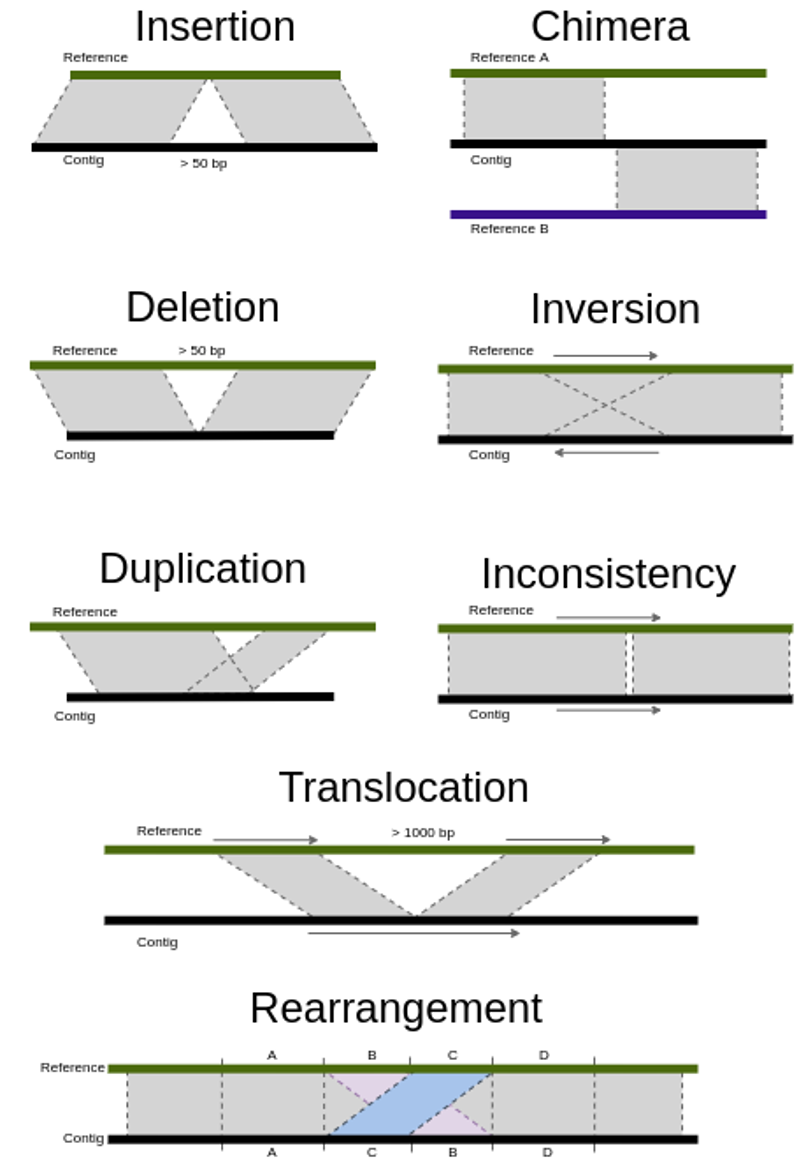
\includegraphics[scale=0.95]{figures/chapter 5/Supplemental Figure 1.png}
\caption{LMAS misassembly classification. Misassembled contigs are classified into 6 main categories: chimera, insertion, deletion, inversion, rearrangement, translocation and duplication, according to the mapping orientation, the distance between blocks in the contig and the mapping coordinates in the reference replicon. If a contig is classified as being chimeric, no further classification is performed. The other categories are classified independently of each other, with combinations being possible, to better reflect the differences in comparison to the reference. If a contig is broken into multiple sequence blocks but fails to be classified in any of the previous categories, it is reported as being inconsistent}
\label{fig:chap5_sup_figure_1}
\end{figure*}

\subsubsection{Per Reference Metrics} \label{ch5_supmaterial_metrics_reference}

\paragraph{General contig information} \mbox{}\\

The following metrics are computed and presented in tabular form: 

\begin{itemize}
    \item \textbf{Contigs:} The total number of contigs in the assembly that align to the reference replicon;
    \item \textbf{Basepairs:} The total number of bases in the assembly that align to the reference replicon;
    \item \textbf{Number of ‘N’s:} Number of uncalled bases (N's) in the contigs that align to the reference replicon.
\end{itemize}

\paragraph{COMPASS} \mbox{}\\

A measure of the quality of a replicon assembly can be considered the proportion of the reference covered by the contigs, i.e. the breadth of coverage of the reference replicon. The COMPASS metrics \cite{bradnam_assemblathon_2013} complement our view of the quality of the assembly with other metrics such as how much redundancy is there in the assembly or the parsimony of the contigs relative to the reference. COMPASS is composed of the following metrics, presented in tabular form:

\begin{itemize}
    \item \textbf{Breadth of Coverage:} Ratio of covered sequence on the reference by aligned contigs;
    \item \textbf{Multiplicity:} Ratio of the length of the alignable assembled sequence to covered sequence on the reference;
    \item \textbf{Validity:} Ratio of the length of the alignable assembled sequence to total basepairs in the aligned contigs;
    \item \textbf{Parsimony:} Cost of the assembly (multiplicity over validity);
\end{itemize}

Additionally, the Breadth of Coverage metric is displayed graphically:

\begin{itemize}
    \item \textbf{Genome Fragmentation:} Scatter plot representing the number of contigs per breadth of coverage of the reference, per assembler.
\end{itemize}

\paragraph{Contiguity} \mbox{}\\

To supplement the traditional NA and NG contiguity metrics implemented in QUAST \cite{gurevich_quast_2013}, we define the LSA metric as the longest single alignment between the assembly and the reference replicon, relative to the reference replicon length, as proposed previously \cite{wick_benchmarking_2021}. This provides a simpler picture of assembly quality as lower contiguity immediately suggests a higher fragmentation, missing sequences or more misassemblies. The following metrics are presented in tabular form:


\begin{itemize}
    \item \textbf{LSA:} longest single alignment between the assembly and the reference, relative to the reference length;
    \item \textbf{NAx (where 0  < x  $\leq$ 100):} Length for which the collection of aligned contigs of that length or longer in an assembly covers at least a given percentage of the total length of the reference replicon;
    \item \textbf{NGx (where 0  < x  $\leq$ 100):} Length for which the collection of aligned contigs of that length or longer covers at least a given percentage of the sequence of the reference.
    \item \textbf{Lx (where 0  < x  $\leq$ 100):} Minimal number of contigs that cover x \% of the sequence of the reference;
\end{itemize}

The NAx, NGx and Lx metrics are presented graphically in a line plot for each value of x, where x represents the percentage of the sequence of the reference, ranging from 0 to 100, per assembler.  

\paragraph{Identity} \mbox{}\\

The identity is defined as the number of exact matches between the contigs and the reference replicon, relative to the reference replicon length. The following metrics are presented in tabular form:

\begin{itemize}
    \item \textbf{Identity:} Ratio of identical basepairs in all aligned contigs to the reference;
    \item \textbf{Lowest identity:} Identity of the lowest scoring contig to the reference;
\end{itemize}

For each plot, the metrics are presented for the contigs filtered for a minimum length that align with the reference replicon.

\begin{itemize}
    \item \textbf{Pls Metric:} Scatter plot for the Phred-like score per contig, per assembler;
    \item \textbf{Gaps: }Location of gaps in comparison to the reference sequence, per assembler, with the cumulative number of gaps per position in the reference. Gaps with 1 basepair or more in length are considered;
    \item \textbf{SNPs:} Location of substitutions in comparison to the reference sequence, per assembler, with the indication of the substitution type and coordinate in the reference. Additionally, the cumulative number of SNPs per position in the reference is presented.
\end{itemize}

\paragraph{Misassembly} \mbox{}\\

Similar to what is performed in Global Metrics, this metric is computed for the filtered set of contigs. An aligned contig is considered misassembled when broken into multiple blocks when mapping to the linear reference replicon. Chimeric contigs aligning to more than one reference replicon are counted in each reference individually. 

\begin{itemize}
    \item \textbf{Misassembled contigs:} Number of aligned contigs that contain a misassembly event;
    \item \textbf{Misassembly events:} Total number of misassemblies in the aligned contigs;
\end{itemize}

Additionally, the following information is shown graphically:

\begin{itemize}
    \item \textbf{Misassemblies:} Location of the alignment blocks of misassembled contigs in comparison to the reference sequence, per assembler, with the cumulative number of basepairs in the alignment blocks per position in the reference.
\end{itemize}

\subsubsection{Computational Performance Metrics} \label{ch5_sup_performance_metrics}

Different software, implementing distinct de novo assembly algorithms, have distinct computational requirements. As such, computational statistics are registered for each assembler. The following metrics are presented in tabular form:

\begin{itemize}
    \item \textbf{Avg Time:} Average run-time formatted as “hour:minute:second”;
    \item \textbf{CPU/Hour:} Average amount of time, in hours, of CPU usage by an assembler. CPU load obtained from the number of CPUs and their usage percentage;
    \item \textbf{Max Memory (GB):} Maximum peak memory usage by the assembler;
    \item \textbf{Average Read (GB):} Average data size read from disk by the assembler;
    \item \textbf{Average Write (GB):} Average data size written to disk by the assembler.
\end{itemize}

Additionally, for reproducibility and traceability purposes, the following information is also registered for each assembler in the table:

\begin{itemize}
    \item \textbf{Version:} Version of the assembler captured from stdout;
    \item \textbf{Container:} Full tag of the container used to run the assembler, with a link to the container location in Docker Hub \cite{noauthor_docker_nodate}.
\end{itemize}

\subsection{LMAS Report}

LMAS comes pre-packaged with the JS source code for the interactive report, available in the resources/ folder. The source code for the report is available in the LMAS.js repository \cite{noauthor_lmas_2021}. It was built with the JavaScript frameworks React \cite{noauthor_react_nodate} (version 16.8.0) and Material-UI \cite{noauthor_mui_nodate} (version 4.11.00). All interactive charts were rendered with the graph visualisation library Plotly.js \cite{noauthor_plotly_nodate} (version 1.57.1) through its React component, react-plotly \cite{noauthor_react_nodate}(version 2.5.0).

\subsection{ZymoBIOMICS microbial community standards} \label{ch5_sup_zymobiomics}

The “get\_data.sh” bash script file provided with LMAS downloads the ZymoBIOMICS Microbial Community Standard data and saves it in the “data” folder, in conformation with the default parameters. The simulated samples and all reference replicons saved in a singular multi-sequence fasta are publicly available in Zenodo under the DOI \url{https://doi.org/10.5281/zenodo.4588969}. 

\subsubsection{Reference Sequences}

The complete bacterial genomes and plasmid sequences for the Microbial Community Standards were obtained from ZymoBIOMICS’ Amazon Simple Storage Service, available at \url{https://s3.amazonaws.com/zymo-files/BioPool/ZymoBIOMICS.STD.refseq.v2.zip}.

For the analysis of LMAS results, the complete ZymoBIOMICS’ reference genomes were annotated with PROKKA \cite{seemann_prokka_2014} (version 1.14.5), using the species-specific database for each reference sequence when available. The number of tRNA, rRNA and mobile element coding genes is available in Supplemental Table \ref{tab:ch5_suptable19}. Pairwise comparisons among the set of reference replicons were conducted by calculating the Average Nucleotide Identity (ANI)  through BLASTn (version 2.12.0) \cite{camacho_blast_2009} using pyani \cite{pritchard_pyani_2022} (version 0.2.11) \cite{pritchard_genomics_2016}. The results are available in Supplemental Table \ref{tab:ch5_suptable23}. 

\subsubsection{Real Sequencing Data}

The real paired-end Illumina sequencing data for the ZymoBIOMICS Microbial Community Standards, both evenly and logarithmic distributed, was obtained from the PRJEB29504 study accession \cite{nicholls_ultra-deep_2019}. The evenly distributed community standard, containing 8.5 million read pairs, is available under the ERR2984773 accession, and the logarithmically distributed sample, containing 47.5 million read pairs, is available under the accession ERR2935805. 

\subsubsection{Mock Sequencing Data}

A set of simulated samples were generated from the genomes in the ZymoBIOMICS standard through the InSilicoSeq sequence simulator (version 1.5.2) \cite{gourle_simulating_2019}, including both even and logarithmic distribution, with and without Illumina error model. The error model was obtained from each corresponding real sample depending on the distribution and used to generate the mock data with matching characteristics, including read number and abundance of species in the community (Supplemental Table \ref{tab:ch5_suptable4}). 

\subsubsection{Mock Sequencing Data}

The taxonomic composition of the ZymoBIOMICS standard samples, both real and mocks was determined through Kraken2 \cite{wood_improved_2019} using the Standard Database (\url{https://genome-idx.s3.amazonaws.com/kraken/k2_standard_20210517.tar.gz}). The following command was used:  “kraken2 --output \$sample.kraken --report \$sample.kraken\_report --memory-mapping --paired --gzip-compressed  \$fastq\_pair[0] \$fastq\_pair[1]” where \$sample is the sample name, \$fastq\_pair[0] contains the forward-facing reads, and \$fastq\_pair[1] the reverse-facing reads.

The processing of the kraken reports was performed through custom python code \cite{noauthor_lmas_2022} where all the percentage of reads that matched for the species in the dataset were saved, as well as the percentage of unclassified reads. For the \textit{Lactobacillus fermentum}, as in the Standard Kraken database no general Species level classification is available, the percentage of reads was calculated as the sum of all reads aligning to one of the \textit{L. fermentum} subspecies. The rest of the reads that were classified as any other species were saved conjunctively as “Other”. Supplemental Table \ref{tab:ch5_suptable20} contains the percentage of classified reads for each of the species in the community, as well as “other” and unclassified reads. 

\subsubsection{Assessment of Assembly Success} \label{ch5_sup_assembly_success}

The complete set of results for 3 LMAS runs for the raw sequence reads of mock communities with an even and logarithmic distribution of species, from real sequencing runs \cite{nicholls_ultra-deep_2019} and simulated read datasets, with and without error, matching the intended distribution of species in each sample for the eight bacterial genomes and four plasmids of the ZymoBIOMICS Microbial Community Standards as reference is available in Supplemental Table \ref{tab:ch5_suptable21} and \ref{tab:ch5_suptable22}. For the assessment of the assembly success for each sample, the different metrics for all LMAS runs were combined and descriptive statistics, such as the average value, standard deviation, minimum and maximum, were obtained through Python’s Pandas describe function \cite{noauthor_pandas_nodate, noauthor_pandasdataframedescribe_nodate}. Both global and reference based for each assembler, each reference replicon and each sample (ENN - evenly distributed without error model; EMS - evenly distributed with Illumina MiSeq error model; ERR2984773 - real evenly distributed Illumina MiSeq sample, LNN - logarithmically distributed without error model; LHS - logarithmically distributed  with Illumina HiSeq error model; ERR2935805 - real logarithmically distributed Illumina HiSeq sample). For descriptive statistics on several assembler by each assembly type (genomic or metagenomic) and each assembler algorithm (single or multiple k-mer), the use of median was preferred due to its higher robustness against outliers and the high range of the distribution of the results. Plotly \cite{noauthor_plotly_nodate} was used to compute the graphs aggregating the results obtained. The jupyter notebooks \cite{noauthor_project_nodate} with the data processing and all resulting files are available at \cite{noauthor_lmas_2022}. 

The top result of each assembler for each sample was selected, based on the following criteria:
\begin{itemize}
    \item For the number of uncalled bases, number of misassembled contigs and number of misassembly events, the lower the value, the better, with the exception of 0 for the number of contigs;
    \item For the percentage of mapped reads and N50, the higher the value, the better; 
    \item The number of basepairs, the best results was the one closest to the target value of the number of basepairs in the reference replicons;
\end{itemize}

For reference-specific metrics, in addition to the ones stated above when applicable (Number of contigs produced, number of uncalled bases, number of misassembled contigs and number of misassembly events), the following criteria were used:

\begin{itemize}
    \item For the L90 metric, the lower value was better, with the exception of 0;
    \item For LSA, NA, NG, breadth of coverage, identity and lowest identity, the higher the value the better;
    \item For multiplicity, parsimony and validity, the closer to 1, the better;
\end{itemize}
 
To obtain the worst value in each metric, the opposite criteria were used. The normalised score for each metric was obtained from the best result for each assembler in each sample through Equation \ref{chap5_sup_eq}. For the assessment of assembler consistency, each contig for each assembler was considered the same as its size was exactly the same in each LMAS run. 

\begin{equation} \label{chap5_sup_eq}
\left\{\begin{matrix}
1 - \frac{x}{min(X)} & \textup{if maximum value is best}\\ 
\frac{x}{min(X)} & \textup{if minimum value is best}\\ 
1 - \frac{|x - T|}{T}\ & \textup{if target value is best}  
\end{matrix}\right.
\end{equation}

Where $x$ is the given value of a metric for an assembler, $X$ the list of values for that metric for all assemblers, and $T$ the target value.

\subsubsection{Resource requirements differ greatly} \label{ch5_sup_resources}

Regarding computational resources, there is a disparity in usage for the evenly and logarithmically distributed samples (Figure \ref{fig:chap5_sup_figure_2}), with the latter having more resource-intensive requirements possibly due mostly to a higher number of reads. The resource usage also varied greatly by assembler, with multiple k-mer dBG (SPAdes, metaSPAdes, MEGAHIT, SKESA, IDBA-UD, GATBMiniaPipeline and Unicycler) having overall higher resource usage. ABySS performance was inconsistent, having reached a maximum of 1412 CPU hours to produce an assembly (sample ERR2984773), resulting in a run time of 35.52 hours.  MetaHipmer2 was the assembler with the highest memory usage, reaching a maximum of 68.7 GB.  

\begin{figure*}[h!]
\centering
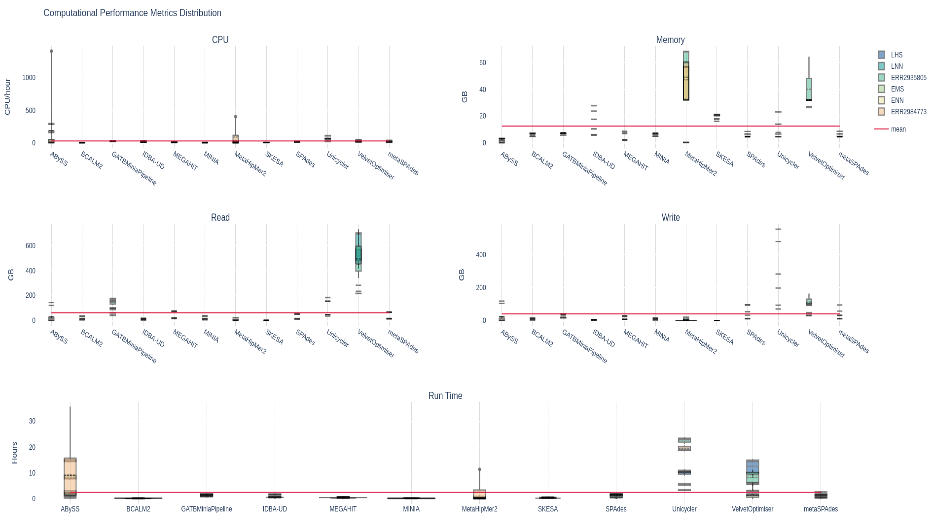
\includegraphics[width=\textwidth]{figures/chapter 5/Supplemental Figure 2.png}
\caption{Computational resources used by each assembler for the evenly and logarithmically distributed samples. Each plot describes the distribution of resource consumption for 3 LMAS runs for the ZymoBIOMICS microbial community standard dataset for the following metrics: A) CPU/hour, B) Maximum memory in GB; C) Data written to disk in GB; D) Data read from dist in GB; E) Run time in hours. The mean for all samples and all assemblers is indicated in red. The samples are indicated as follows: ENN: dark blue, EMS: teal, ERR2984773: green, LNN: light green, LHS: yellow, ERR2935805: light orange. }
\label{fig:chap5_sup_figure_2}
\end{figure*}

\begin{figure*}[]
\centering
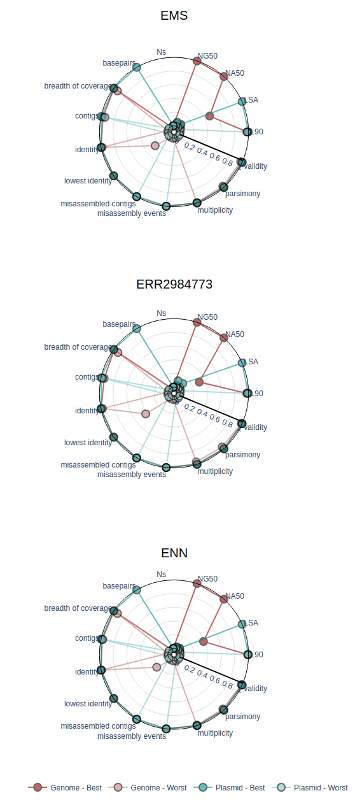
\includegraphics[scale=0.95]{figures/chapter 5/Supplemental Figure 3.png}
\caption{Performance per reference of genomic and metagenomic assemblers for the evenly distributed samples in the ZymoBIOMICS Microbial Community Standards dataset. For each sample in the dataset and for the 3 runs, the best and worst scores for each assembler category were selected: genomic (in blue) and metagenomic (in red). The results for each global assembly metric was normalised, with 1 representing the best result, and 0 the worst.}
\label{fig:chap5_sup_figure_3}
\end{figure*}

\begin{figure*}[]
\centering
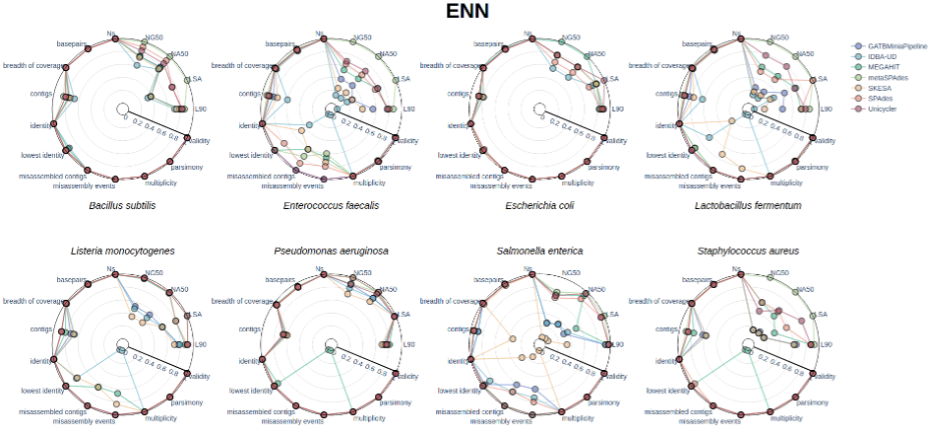
\includegraphics[width=\textwidth]{figures/chapter 5/Supplemental Figure 4.png}
\caption{Assembler performance per reference for the ZymoBIOMICS Microbial Community Standards dataset for sample ENN. The best score for each assembler was selected for 3 LMAS runs. The results for each global assembly metric was normalised, with 1 representing the best result, and 0 the worst. The following assemblers are represented: GATBMiniaPipeline: dark blue, IDBA-UD: light blue, MEGAHIT: dark green, metaSPAdes: light green, SKESA: yellow, SPAdes: orange, Unicycler: red.}
\label{fig:chap5_sup_figure_4}
\end{figure*}

\begin{figure*}[]
\centering
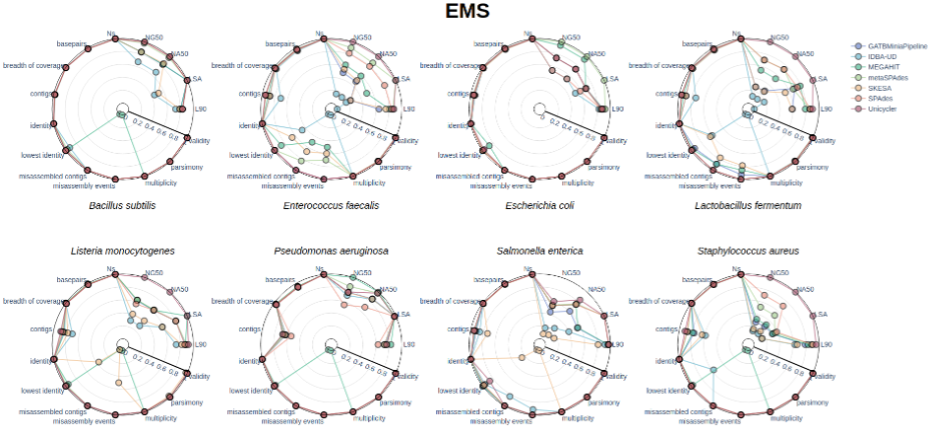
\includegraphics[width=\textwidth]{figures/chapter 5/Supplemental Figure 5.png}
\caption{Assembler performance per reference for the ZymoBIOMICS Microbial Community Standards dataset for sample EMS. The best score for each assembler was selected for 3 LMAS runs. The results for each global assembly metric was normalised, with 1 representing the best result, and 0 the worst. The following assemblers are represented: GATBMiniaPipeline: dark blue, IDBA-UD: light blue, MEGAHIT: dark green, metaSPAdes: light green, SKESA: yellow, SPAdes: orange, Unicycler: red.}
\label{fig:chap5_sup_figure_5}
\end{figure*}

\begin{figure*}[]
\centering
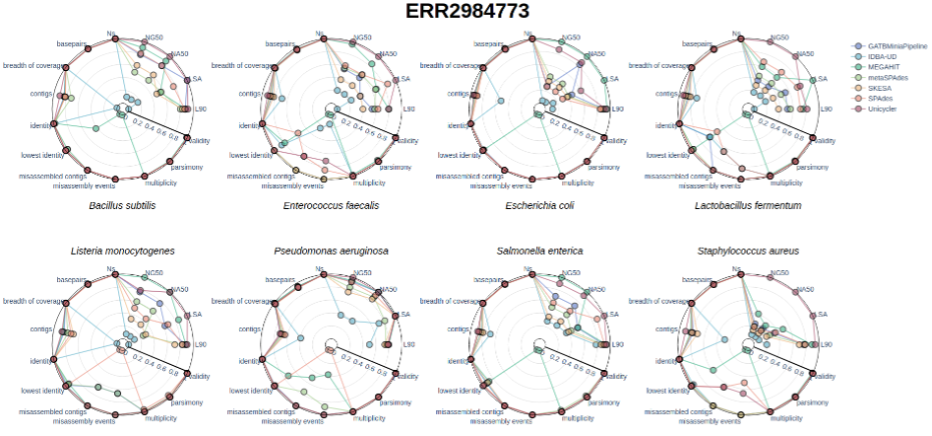
\includegraphics[width=\textwidth]{figures/chapter 5/Supplemental Figure 6.png}
\caption{Assembler performance per reference for the ZymoBIOMICS Microbial Community Standards dataset for sample ERR2984773. The best score for each assembler was selected for 3 LMAS runs. The results for each global assembly metric was normalised, with 1 representing the best result, and 0 the worst. The following assemblers are represented: GATBMiniaPipeline: dark blue, IDBA-UD: light blue, MEGAHIT: dark green, metaSPAdes: light green, SKESA: yellow, SPAdes: orange, Unicycler: red.}
\label{fig:chap5_sup_figure_6}
\end{figure*}

\begin{figure*}[]
\centering
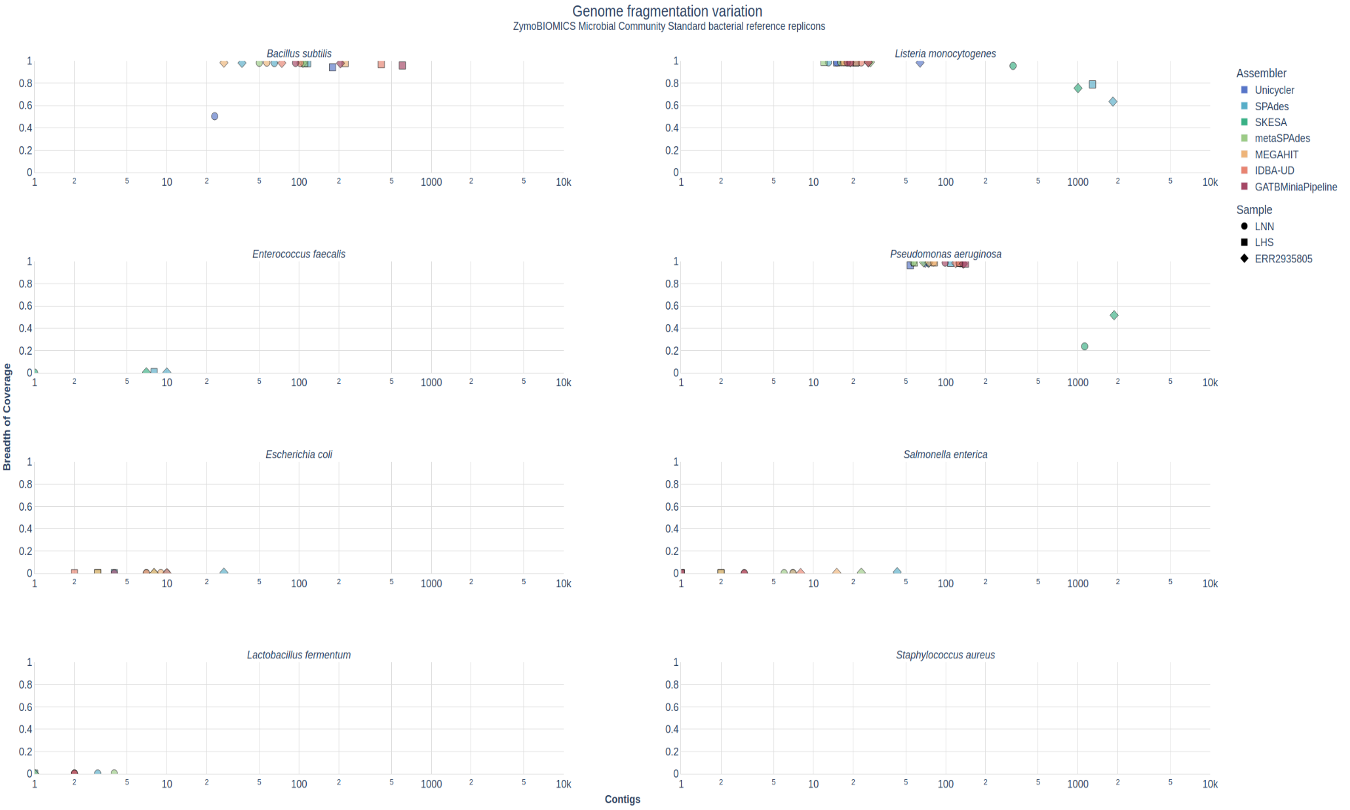
\includegraphics[width=\textwidth]{figures/chapter 5/Supplemental Figure 7.png}
\caption{Genome fragmentation for each reference replicon of the ZimoBIOMICS community standards dataset for the logarithmically distributed samples. Genome fragmentation for the 3 LMAS runs is represented by the number of contigs and breadth of coverage of the reference per assembler for the logarithmically distributed samples: LNN (logarithmically distributed without error model, identified by a circle), LHS (logarithmically distributed with Illumina HiSeq error model, identified by a square) and ERR2935805 (real Illumina HiSeq sample, identified by a diamond). Each assembler is identified with the following colour scheme - dark blue: Unicycler, light blue: SPAdes, dark green: SKESA, light green: metaSPAdes, yellow: MEGAHIT, orange: IDBA-UD, red: GATBMiniaPipeline.}
\label{fig:chap5_sup_figure_7}
\end{figure*}

\begin{figure*}[]
\centering
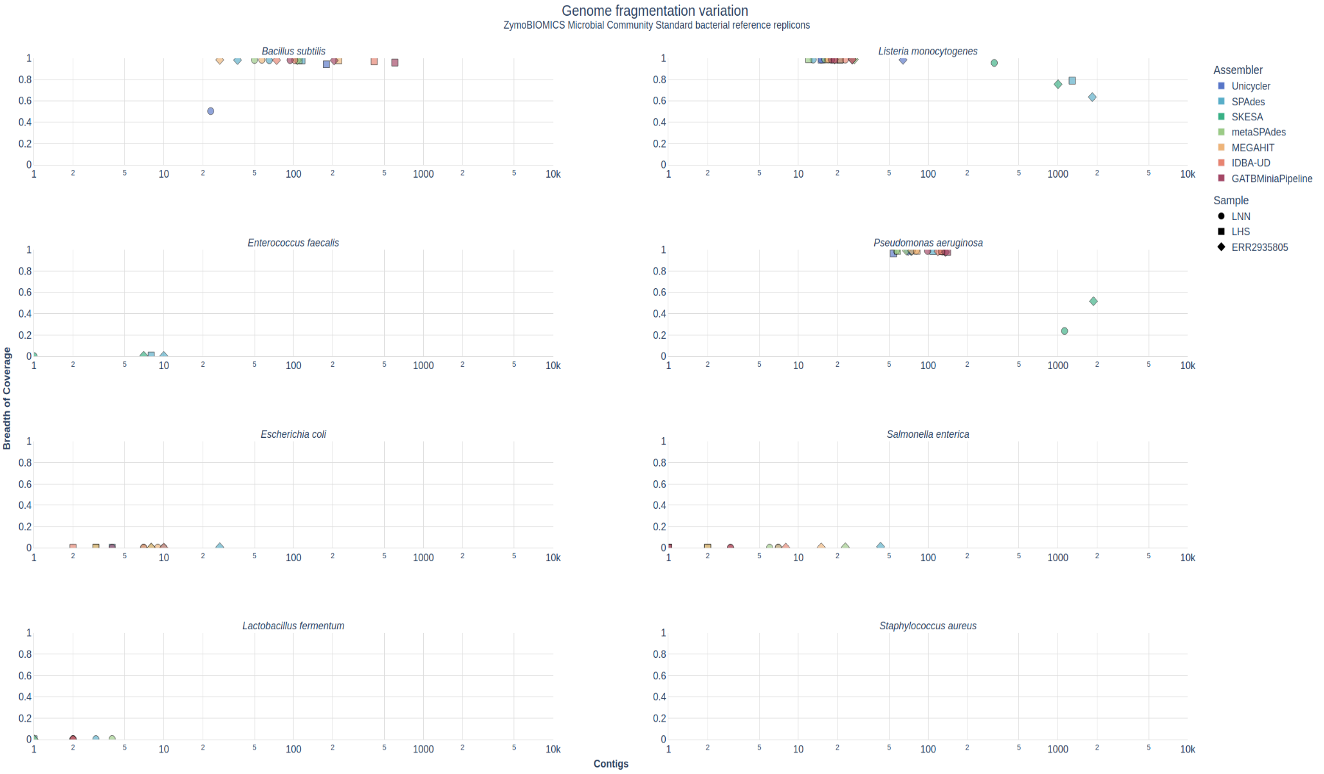
\includegraphics[width=\textwidth]{figures/chapter 5/Supplemental Figure 8.png}
\caption{Genome fragmentation for each reference replicon of the BMock12 community standards dataset sample. Genome fragmentation is represented by the number of contigs and breadth of coverage of the reference per assembler. Each assembler is identified with the following colour scheme - dark blue: Unicycler, light blue: SPAdes, dark green: SKESA, light green: metaSPAdes, yellow: MEGAHIT, orange: IDBA-UD, red: GATBMiniaPipeline. Each reference replicon is identified by its IMG Taxon ID: 2615840527, Muricauda sp; 2615840533, Thioclava sp; 2615840601, Cohaesibacter sp; 2615840646, Propionibacteriaceae bacterium, 2615840697, Marinobacter sp LV10R510-8; 2616644829, Marinobacter sp LV10MA510-1; 2617270709, Psychrobacter sp; 2623620557, Micromonospora echinaurantiaca; 2623620567, Micromonospora echinofusca; 2623620609, Micromonospora coxensis; 2623620617, Halomonas sp. HL-4; and 2623620618, Halomonas sp. HL-93. }
\label{fig:chap5_sup_figure_8}
\end{figure*}

\begin{figure*}[]
\centering
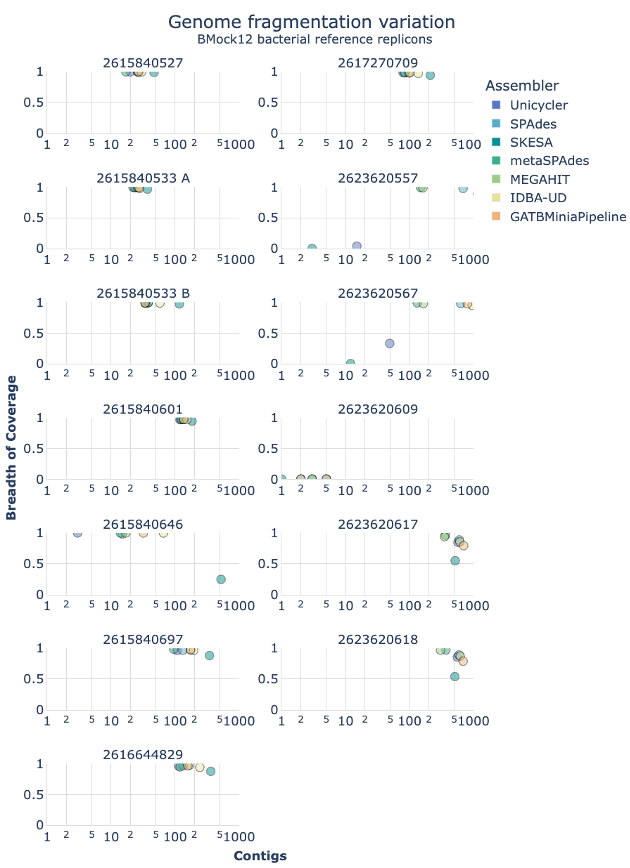
\includegraphics[width=\textwidth]{figures/chapter 5/Supplemental Figure 9.png}
\caption{Location of gaps in comparison to the reference sequence, per assembler, for each reference replicon of the BMock12 community standards datasets. The resulting plot contains the gaps obtained for GATBMiniaPipeline, IDBA-UD, MEGAHIT, metaSPAdes, SKESA, SPAdes and Unicycler assemblers.}
\label{fig:chap5_sup_figure_9}
\end{figure*}


\newpage

\begin{table}[]
\centering
\caption{Tools available for the de novo assembly of prokaryotic genomes. For each tool, its publication is indicated, if available, as well as the assembly algorithm implemented if it was developed explicitly to handle metagenomic datasets. The tools are ordered by the date of the last update, with the source code indicated when available. The tools incorporated in LMAS are indicated as such. }
\label{tab:ch5_suptable1}
Table available for download at \url{https://zenodo.org/record/6623458/files/LMAS\%20Supplemental\%20Material\%20-\%20Tables_Table\%20S1.xlsx}
\end{table}
\begin{table}[]
\centering
\caption{Comparison of metrics and features of LMAS with QUAST and MetaQUAST.}
\label{tab:ch5_suptable2}
Table available for download at \url{https://zenodo.org/record/6623458/files/LMAS\%20Supplemental\%20Material\%20-\%20Tables_Table\%20S2.xlsx}
\end{table}
\begin{scriptsize}
\begin{center}

\begin{table}[]
\centering
\caption{The ZymoBIOMICS Microbial Community Standard datasets. Set of raw sequence reads used as input in LMAS  of mock communities with an even and logarithmic distribution of species, from real sequencing runs and simulated read datasets, with and without error, matching the intended distribution of species in ZymoBIOMICS Microbial Community Standard.}
\label{tab:ch5_suptable3}
\resizebox{\textwidth}{!}{%
\begin{tabular}{@{}lllll@{}}
\toprule
Sample   Name & Distribution & Error Model         & Read Length (bp) & Read Pairs (M) \\ \midrule
ENN           & Even         & None                & 150              & 8,5            \\
EMS           & Even         & Illumina   MiSeq    & 150              & 8,5            \\
ERR2984773    & Even         & Real   MiSeq Sample & 150              & 8,5            \\
LNN           & Log          & None                & 100              & 47,5           \\
LHS           & Log          & Illumina   HiSeq    & 100              & 47,5           \\
ERR2935805    & Log          & Real   HiSeq Sample & 100              & 47,5           \\ \bottomrule
\end{tabular}%
}
\end{table}

\end{center}
\end{scriptsize}

\begin{table}[]
\centering
\caption{Microbial composition of the ZymoBIOMICS microbial community standard dataset with Even and Logarithmic distribution of species. Theoretical microbial composition of the standards, and the corresponding number of reads generated for each replicon.}
\label{tab:ch5_suptable4}
Table available for download at \url{https://zenodo.org/record/6623458/files/LMAS\%20Supplemental\%20Material\%20-\%20Tables_Table\%20S4.xlsx}
\end{table}
\begin{table}[]
\centering
\caption{Global quality metrics variation in three LMAS runs for sample ENN per assembler. The average calculated for all samples in the dataset for the 3 independent LMAS runs, followed by the minimum and maximum values obtained, are presented for each metric for each assembler.}
\label{tab:ch5_suptable5}
Table available for download at \url{https://zenodo.org/record/6623458/files/LMAS\%20Supplemental\%20Material\%20-\%20Tables_Table\%20S5.xlsx}
\end{table}
\begin{table}[]
\centering
\caption{Global quality metrics variation in three LMAS runs for sample EMS per assembler. The average calculated for all samples in the dataset for the 3 independent LMAS runs, followed by the minimum and maximum values obtained, are presented for each metric for each assembler.}
\label{tab:ch5_suptable6}
Table available for download at \url{https://zenodo.org/record/6623458/files/LMAS\%20Supplemental\%20Material\%20-\%20Tables_Table\%20S6.xlsx}
\end{table}
\begin{table}[]
\centering
\caption{Global quality metrics variation in three LMAS runs for sample ERR2984773 per assembler. The average calculated for all samples in the dataset for the 3 independent LMAS runs, followed by the minimum and maximum values obtained, are presented for each metric for each assembler.}
\label{tab:ch5_suptable7}
Table available for download at \url{https://zenodo.org/record/6623458/files/LMAS\%20Supplemental\%20Material\%20-\%20Tables_Table\%20S7.xlsx}
\end{table}
\begin{table}[]
\centering
\caption{Global quality metrics variation in three LMAS runs for sample LNN per assembler. The average calculated for all samples in the dataset for the 3 independent LMAS runs, followed by the minimum and maximum values obtained, are presented for each metric for each assembler.}
\label{tab:ch5_suptable8}
Table available for download at \url{https://zenodo.org/record/6623458/files/LMAS\%20Supplemental\%20Material\%20-\%20Tables_Table\%20S8.xlsx}
\end{table}
\begin{table}[]
\centering
\caption{Global quality metrics variation in three LMAS runs for sample LHS per assembler. The average calculated for all samples in the dataset for the 3 independent LMAS runs, followed by the minimum and maximum values obtained, are presented for each metric for each assembler.}
\label{tab:ch5_suptable9}
Table available for download at \url{https://zenodo.org/record/6623458/files/LMAS\%20Supplemental\%20Material\%20-\%20Tables_Table\%20S9.xlsx}
\end{table}
\begin{table}[]
\centering
\caption{Global quality metrics variation in three LMAS runs for sample ERR2935805 per assembler. The average calculated for all samples in the dataset for the 3 independent LMAS runs, followed by the minimum and maximum values obtained, are presented for each metric for each assembler.}
\label{tab:ch5_suptable10}
Table available for download at \url{https://zenodo.org/record/6623458/files/LMAS\%20Supplemental\%20Material\%20-\%20Tables_Table\%20S10.xlsx}
\end{table}

\begin{scriptsize}
\begin{center}

\begin{table}[]
\centering
\caption{Inconsistent contigs produced by the assemblers in 3 LMAS runs. For each assembler, the total number of contigs produced over the 3 runs of the LMAS workflow is indicated, as well as the contigs present in only two and a single run. }
\label{tab:ch5_suptable11}
\resizebox{\textwidth}{!}{%
\begin{tabular}{@{}lllll@{}}
\toprule
Assembler &
  Total Contigs &
  \begin{tabular}[c]{@{}l@{}}Contigs present in \\ 3 out of 3 runs\end{tabular} &
  \begin{tabular}[c]{@{}l@{}}Contigs present in \\ 2 out of 3 runs\end{tabular} &
  \begin{tabular}[c]{@{}l@{}}Contigs present in \\ 1 out of 3 runs\end{tabular} \\ \midrule
ABySS             & 7638  & 2505 & 50  & 23  \\
BCALM2            & 1962  & 654  & 0   & 0   \\
GATBMiniaPipeline & 14321 & 4753 & 25  & 12  \\
IDBA-UD           & 15383 & 5115 & 16  & 6   \\
MEGAHIT           & 5440  & 1812 & 1   & 2   \\
MetaHipMer2       & 2358  & 772  & 16  & 10  \\
metaSPAdes        & 6462  & 2154 & 0   & 0   \\
minia             & 6427  & 2106 & 41  & 27  \\
SKESA             & 11187 & 3729 & 0   & 0   \\
SPAdes            & 8631  & 2877 & 0   & 0   \\
Unicycler         & 5598  & 1866 & 0   & 0   \\
VelvetOptimiser   & 2315  & 553  & 112 & 432 \\
\bottomrule
\end{tabular}%
}
\end{table}

\end{center}
\end{scriptsize}
\begin{table}[]
\centering
\caption{Global assembly metrics for single and multiple k-mer dBg assemblers. The median and the minimum and maximum values obtained are presented for each metric for all samples in 3 runs of LMAS. Single k-mer bBg assemblers: ABySS, BCALM2 and minia. Multiple k-mer bBg assembler: GATBMiniaPipeline, IDBA-UD, MEGAHIT, MetaHipMer2, metaSPAdes, SKESA, SPAdes, Unicycler and VelverOptimiser.}
\label{tab:ch5_suptable12}
Table available for download at \url{https://zenodo.org/record/6623458/files/LMAS\%20Supplemental\%20Material\%20-\%20Tables_Table\%20S12.xlsx}
\end{table}
\begin{table}[]
\centering
\caption{Global assembly metrics for genomic and metagenomic multiple k-mer dBg assemblers. The median and the minimum and maximum values obtained are presented for each metric for all samples in 3 runs of LMAS. Genomic assemblers: SKESA, SPAdes and Unicycler. Metagenomic assemblers: GATBMiniaPipeline, IDBA-UD, MEGAHIT and metaSPAdes.}
\label{tab:ch5_suptable13}
Table available for download at \url{https://zenodo.org/record/6623458/files/LMAS\%20Supplemental\%20Material\%20-\%20Tables_Table\%20S13.xlsx}
\end{table}
\begin{table}[]
\centering
\caption{Per reference quality metrics variation in three LMAS s for sample ENN per assembler of the ZymoBIOMICS microbial community standard dataset. The average calculated for all samples in the dataset for the 3 independent LMAS runs, followed by the minimum and maximum values obtained, are presented for each metric for each assembler.}
\label{tab:ch5_suptable14}
Table available for download at \url{https://zenodo.org/record/6623458/files/LMAS\%20Supplemental\%20Material\%20-\%20Tables_Table\%20S14.xlsx}
\end{table}
\begin{table}[]
\centering
\caption{Per reference quality metrics variation in three LMAS s for sample EMS per assembler of the ZymoBIOMICS microbial community standard dataset. The average calculated for all samples in the dataset for the 3 independent LMAS runs, followed by the minimum and maximum values obtained, are presented for each metric for each assembler.}
\label{tab:ch5_suptable15}
Table available for download at \url{https://zenodo.org/record/6623458/files/LMAS\%20Supplemental\%20Material\%20-\%20Tables_Table\%20S15.xlsx}
\end{table}
\begin{table}[]
\centering
\caption{Per reference quality metrics variation in three LMAS s for sample ERR2984773 per assembler of the ZymoBIOMICS microbial community standard dataset. The average calculated for all samples in the dataset for the 3 independent LMAS runs, followed by the minimum and maximum values obtained, are presented for each metric for each assembler.}
\label{tab:ch5_suptable16}
Table available for download at \url{https://zenodo.org/record/6623458/files/LMAS\%20Supplemental\%20Material\%20-\%20Tables_Table\%20S16.xlsx}
\end{table}
\begin{scriptsize}
\begin{center}

\begin{table}[]
\centering
\caption{Inconsistent gaps produced by the assemblers in 3 LMAS runs. For each assembler, the total number of gaps consistently produced in relation to the reference replicons over the 3 runs of the LMAS workflow is indicated, as well as gaps present in only two and a single run.}
\label{tab:ch5_suptable17}
\resizebox{\textwidth}{!}{%
\begin{tabular}{@{}llll@{}}
\toprule
Assembler &
  \begin{tabular}[c]{@{}l@{}}Gaps present in \\ 3 out of 3 runs\end{tabular} &
  \begin{tabular}[c]{@{}l@{}}Gaps present in \\ 2 out of 3 runs\end{tabular} &
  \begin{tabular}[c]{@{}l@{}}Gaps present in \\ 1 out of 3 runs\end{tabular} \\ \midrule
GATBMiniaPipeline & 3108 & 278 & 157 \\
IDBA-UD           & 4458 & 68  & 40  \\
MEGAHIT           & 1017 & 122 & 89  \\
metaSPAdes        & 1185 & 0   & 0   \\
SKESA             & 6681 & 0   & 0   \\
SPAdes            & 2433 & 0   & 0   \\
Unicycler         & 1512 & 0   & 0  \\\bottomrule
\end{tabular}%
}
\end{table}

\end{center}
\end{scriptsize}
\begin{table}[]
\centering
\caption{Annotation of consistent gaps produced by the assemblers in 3 LMAS runs.}
\label{tab:ch5_suptable18}
Table available for download at \url{https://zenodo.org/record/6623458/files/LMAS\%20Supplemental\%20Material\%20-\%20Tables_Table\%20S18.xlsx}
\end{table}
\begin{scriptsize}
\begin{center}

\begin{table}[]
\centering
\caption{Number of tRNA and rRNA coding sequencing, and mobile elements in ZymoBIOMICS microbial community standard reference replicons. The average calculated for all samples in the dataset for the 3 independent LMAS runs, followed by the minimum and maximum values obtained, are presented for each metric for each assembler. }
\label{tab:ch5_suptable19}
\resizebox{\textwidth}{!}{%
\begin{tabular}{@{}llll@{}}
\toprule
Reference               & tRNA & rRNA & Mobile elements \\\midrule
\textit{Bacillus subtilis}       & 86   & 31   & 17              \\
\textit{Enterococcus faecalis}   & 62   & 12   & 7               \\
\textit{Escherichia coli}        & 89   & 22   & 85              \\
\textit{Lactobacillus fermentum} & 59   & 15   & 80              \\
\textit{Listeria monocytogenes}  & 67   & 18   & 3               \\
\textit{Pseudomonas aeruginosa}  & 78   & 12   & 19              \\
\textit{Salmonella enterica}     & 88   & 22   & 39              \\
\textit{Staphylococcus aureus}   & 60   & 19   & 7              \\\bottomrule
\end{tabular}%
}
\end{table}

\end{center}
\end{scriptsize}
\begin{table}[]
\centering
\caption{Taxonomic classification of the ZymoBIOMICS microbial community standard dataset. The classification was performed with Kraken2, using the Standard Database. The results are presented as the percentage of classified reads for the 8 bacterial species in the community, as well as unclassified reads and the group of reads that are classified as species not contained in the community standard.}
\label{tab:ch5_suptable20}
Table available for download at \url{https://zenodo.org/record/6623458/files/LMAS\%20Supplemental\%20Material\%20-\%20Tables_Table\%20S20.xlsx}
\end{table}
\begin{table}[]
\centering
\caption{Global assembly metrics for dBg assemblers with single and multiple k-mer algorithms.}
\label{tab:ch5_suptable21}
Table available for download at \url{https://zenodo.org/record/6623458/files/LMAS\%20Supplemental\%20Material\%20-\%20Tables_Table\%20S21.xlsx}
\end{table}
\begin{table}[]
\centering
\caption{Reference based quality metrics in three LMAS runs for the ZimoBIOMICS community standards dataset.}
\label{tab:ch5_suptable22}
Table available for download at \url{https://zenodo.org/record/6623458/files/LMAS\%20Supplemental\%20Material\%20-\%20Tables_Table\%20S22.xlsx}
\end{table}
\begin{table}[]
\centering
\caption{Pairwise comparisons of the ZymoBIOMICS microbial community standard reference replicons. All pairwise comparisons among the set of genomes were conducted using Average Nucleotide Identity through BLAST as a proxy for DNA-DNA hybridisation.}
\label{tab:ch5_suptable23}
Table available for download at \url{https://zenodo.org/record/6623458/files/LMAS\%20Supplemental\%20Material\%20-\%20Tables_Table\%20S23.xlsx}
\end{table}
\begin{table}[]
\centering
\caption{Microbial composition of the BMock12 microbial community standard dataset.}
\label{tab:ch5_suptable24}
Table available for download at \url{https://zenodo.org/record/7129554/files/LMAS\%20Supplemental\%20Material\%20-\%20Tables\%20-\%20revision_Table\%20S24.xlsx}
\end{table}
\begin{table}[]
\centering
\caption{Pairwise comparisons of the BMock12 microbial community standard reference replicons.}
\label{tab:ch5_suptable25}
Table available for download at \url{https://zenodo.org/record/7129554/files/LMAS\%20Supplemental\%20Material\%20-\%20Tables\%20-\%20revision_Table\%20S25.xlsx}
\end{table}
\begin{table}[]
\centering
\caption{ Global quality metrics  for the BMock12 sample SRX4901583 per assembler.}
\label{tab:ch5_suptable26}
Table available for download at \url{https://zenodo.org/record/7129554/files/LMAS\%20Supplemental\%20Material\%20-\%20Tables\%20-\%20revision_Table\%20S26.xlsx}
\end{table}
\begin{table}[]
\centering
\caption{ Per reference quality metrics  for the BMock12 sample SRX4901583 per assembler.}
\label{tab:ch5_suptable27}
Table available for download at \url{https://zenodo.org/record/7129554/files/LMAS\%20Supplemental\%20Material\%20-\%20Tables\%20-\%20revision_Table\%20S27.xlsx}
\end{table}
\begin{table}[]
\centering
\caption{Microbial composition of the Gut-Mix-RR microbial community standard dataset.}
\label{tab:ch5_suptable28}
Table available for download at \url{https://zenodo.org/record/7129554/files/LMAS\%20Supplemental\%20Material\%20-\%20Tables\%20-\%20revision_Table\%20S28.xlsx}
\end{table}
\begin{table}[]
\centering
\caption{Pairwise comparisons of the Gut-Mix microbial community standard reference replicons.}
\label{tab:ch5_suptable29}
Table available for download at \url{https://zenodo.org/record/7129554/files/LMAS\%20Supplemental\%20Material\%20-\%20Tables\%20-\%20revision_Table\%20S29.xlsx}
\end{table}
\begin{table}[]
\centering
\caption{Global quality metrics  for the Gut-Mix-RR sample SRR11487941 per assembler.}
\label{tab:ch5_suptable30}
Table available for download at \url{https://zenodo.org/record/7129554/files/LMAS\%20Supplemental\%20Material\%20-\%20Tables\%20-\%20revision_Table\%20S30.xlsx}
\end{table}
\newpage
\section{References}
\printbibliography[heading=none]
\end{refsection}


%-----------------------------------------------------------------
% Paper 5 - hAMRonization
%------------------------------------------------------------------
\newpage
\thispagestyle{empty}
\chapter{hAMRonization: Enhancing antimicrobial resistance prediction using PHA4GE standards and specification\label{ch:paper5}}

\thispagestyle{empty}
\clearpage \thispagestyle{empty}\mbox{}\clearpage
\newpage
\begin{refsection}
%\mbox{}\\
\vspace{8cm}


This chapter is a reproduction of the following submitted manuscript for publication in eLife:

C. I. Mendes, F. Maguire, A. Manuele, D. Fornika, S. Tausch, T. Le-Viet, J. Phelan, C. Meehan, A. Raphenya, B. Alcock, E. Culp, A. McArthur, M. Feldgarden, G. Tyson, M. Galas, J. Campos, A. Witney, D. Aanensen, A. Black, L. Katz, P. Oluniyi, I. Olawoye, R. Timme, A. T. Vasconcelos, A. Page, D. MacCannell, E. Griffiths. 
hAMRonization: Enhancing antimicrobial resistance prediction using PHA4GE standards and specification

My contribution to this publication included the development of the antimicrobial detection contextual data specification package, including it’s conversion and availability in a machine-applicable JSON format. It also includes the design and implementation of the hAMRonization package, results analysis, manuscript production and editing. 

\cleardoublepage 

\begin{center}
\large
\textbf{hAMRonization: Enhancing antimicrobial resistance  prediction using PHA4GE standards and specification}
\end{center}

F Maguire$^{1,*}$,
Catarina I Mendes$^{2,*}$, 
A Manuele, 
D Fornika, 
S H Tausch, 
T Le-Viet, 
A R Raphenya, 
B Alcock, 
E Culp, 
A G McArthur, 
M Feldgarden, 
G H Tyson, 
M Galas, 
J Campos, 
A A Witney, 
D M Aanensen, 
A Black, 
E Hodcroft, 
L S Katz, 
P E Oluniyi, 
I B Olawoye, 
R E Timme, 
A T R Vasconcelos, 
A J Page, 
D R MacCannell, 
E J Griffiths, 
on behalf of the Public Health Alliance for Genomic Epidemiology (PHA4GE) consortium Data Structures Working Group

$^1$ 

$^2$Instituto de Microbiologia, Instituto de Medicina Molecular, Faculdade de Medicina, Universidade de Lisboa, Lisboa, Portugal 

$^*$ Contributed equally 

\section{Abstract}

The detection of antimicrobial resistance (AMR) directly from genomic or metagenomic data has become a standard procedure in public health, with a large number of different bioinformatic tools currently available to perform this task. These tools, although implementing similar principles, differ in supported inputs, search algorithms, parameterisation, and underlying reference databases. Each of these tools generates a report of detected AMR genes or variants in a distinct, non-standard, format. This is a huge barrier to the comparison of results and the modularity of tools within bioinformatic workflows. 

The Public Health Alliance for Genomic Epidemiology (PHA4GE) (\url{https://pha4ge.org}) has developed a standardized output specification for the bioinformatic detection of AMR from genomes. hAMRonization, a python package and command-line utility, implements PHA4GE’s AMR specification to combine the outputs of disparate antimicrobial resistance gene detection tools into a single unified format.  hAMRonization can be easily extended, currently supporting XX different  tools, both species-agnostic and species-specific, for the detection of genes and/or variants conferring AMR. The harmonized reports are available in tabular form, JSON or through an interactive HTML file that can be opened within the browser for navigable data exploration. The hAMRonization and underlying specification are open-source and freely available through PyPI, conda and GitHub (\url{https://github.com/pha4ge/hAMRonization}).

\subsubsection{Keywords}

interoperability; antimicrobial resistance; public health; workflows

\section{Introduction}

Antimicrobial resistance (AMR) represents a present and growing public health crisis with a global impact.  Multidrug resistance is increasing in a broad range of pathogens \cite{aslam_antibiotic_2018}; combined with low rates of antimicrobial drug discovery \cite{brown_antibacterial_2016} this represents a threat to human and animal health \cite{who_who_2015}. National and international action plans e.g., \cite{jim_oneill_antimicrobial_2014, jim_oneill_tackling_2016, public_health_agency_of_canada_antimicrobial_2014, who_who_2015}, have identified several strategies to mitigate the risk of AMR such as rapid diagnosis of the AMR determinants present within a clinical sample, improved surveillance of AMR, and gaining a better understanding of the mechanisms of environmental AMR transmission.

Diagnostic and public health surveillance analyses are increasingly performed using genomic and metagenomic data \cite{mcarthur_antimicrobial_2017}. Therefore, accurate identification of genes or variants from genomic data which are predicted to confer resistance to antimicrobials is critical for monitoring and attempting to mitigate the spread of AMR. This work is being performed all over the world by public health agencies, clinicians, industry, and academic researchers. Given the scale of this problem and the number of stakeholders involved, many bioinformatics tools have been developed that are dedicated to the task of AMR gene and variant detection \cite{boolchandani_sequencing-based_2019, hendriksen_using_2019, mcarthur_antimicrobial_2017}. 

These tools include several developed to work with a specific primary database, e.g., the Resistance Gene Identifier (RGI) for the Comprehensive Antibiotic Resistance Database (CARD)\cite{alcock_card_2020}, AMRFinderPlus and the National Center for Biotechnology Information (NCBI) Pathogen Detection Reference Gene catalogue \cite{feldgarden_validating_2019}, and ResFinder and KmerResistance \cite{clausen_benchmarking_2016} for the ResFinder database \cite{zankari_identification_2012}. Other tools exist that use merged forms of existing databases such as ResFams \cite{gibson_improved_2015}, AMRplusplus \cite{doster_megares_2020}, and DeepARG \cite{arango-argoty_deeparg_2018}. Finally, there are AMR gene identification tools that provide a database-agnostic approach using novel algorithms (e.g., GROOT \cite{rowe_indexed_2018}, ARIBA \cite{hunt_ariba_2017}), or a different interface (e.g., ABRicate \cite{torsten_seeman_abricate_2020}, sraX \cite{panunzi_srax_2020}). 

These tools all have different strengths and weaknesses attributable to varied underlying databases, search algorithms, and default parameterisations.  Based on the specific requirements of a given AMR analysis context one tool may be better suited in the analytical workflow than another.    

Unfortunately, all these tools also generate differently formatted outputs using divergent terminology.  This poses a significant challenge to effective integration, modularity, and comparison of AMR gene detection methods.  The consequence of this is that it is difficult for researchers and public health experts to systematically evaluate the suitability of different tools in their workflow. With the limited examples of these comparisons largely reliant on development of custom ad-hoc tool-specific parsers, e.g., \cite{feldgarden_validating_2019, hunt_ariba_2017}), or has skipped the tools entirely and directly compared the underlying algorithms e.g., \cite{mccall_comparative_2018}. Even in cases where benchmarking has been performed, the disparate output formats means it requires significant work to modify a workflow to use a different AMR detection tool. This greatly limits modularity and flexibility to integrate new tools into existing analyses or repurpose them to new or changing requirements. Given the recent calls to mitigate these issues in public health genomic epidemiology \cite{black_ten_2020}, it is critical that data structures and methods are developed which enable tool-agnostic, robust parsing, manipulation, and transformation of AMR gene detection results.

To this end, we compared and consolidated the outputs of existing AMR gene detection tools to develop the hAMRonization specification. This is a standardised set of recommended and mandatory output terms and labels for AMR gene detection tools, such as “Gene Name”, “\% Coverage (breadth)”, and “Drug Class”.  The outputs for all currently maintained, general purpose, AMR gene detection tools can be directly converted to this unified specification.  Furthermore, this conversion to a common AMR gene detection output specification can be performed automatically using a companion library of biopython compatible parsers.


\newpage
\section{References}
\printbibliography[heading=none]
\end{refsection}

%-----------------------------------------------------------------
% Paper 6 - SARS-CoV-2
%------------------------------------------------------------------
\newpage
\thispagestyle{empty}
\chapter{Future-proofing and maximising the utility of metadata: The PHA4GE SARS-CoV-2 contextual data specification package\label{ch:paper6}}

\thispagestyle{empty}
\clearpage \thispagestyle{empty}\mbox{}\clearpage
\newpage
\begin{refsection}
\mbox{}\\
\vspace{8cm}

This chapter is a reproduction of the following publication:

E. J. Griffiths, R. E. Timme, C. I. Mendes, A. J. Page, N. Alikhan, D. Fornika, F. Maguire, J. Campos, D. Park, I. B. Olawoye, P. E. Oluniyi, D. Anderson, A. Christoffels, A. G. da Silva, R. Cameron, D. Dooley, L. S. Katz, A. Black, I. Karsch-Mizrachi, T. Barrett, A. Johnston, T. R. Connor, S. M. Nicholls, A. A. Witney, G. H. Tyson, S. H. Tausch, A. R. Raphenya, B. Alcock, D. M. Aanensen, E. Hodcroft, W. W. L. Hsiao, A. T. R. Vasconcelos, D. R. MacCannell on behalf of the Public Health Alliance for Genomic Epidemiology (PHA4GE) consortium.
Future-proofing and maximizing the utility of metadata: The PHA4GE SARS-CoV-2 contextual data specification package. GigaScience, Volume 11, giac003 (2022). DOI: \url{https://doi.org/10.1093/gigascience/giac003}

The supplementary information referred throughout the text can be consulted in this chapter before the section of references. 

TO CONTINUEEEEE

\cleardoublepage 

\begin{center}
\large
\textbf{Future-proofing and maximizing the utility of metadata: The PHA4GE SARS-CoV-2 contextual data specification package}
\end{center}

Emma J. Griffiths$^1$, 
Ruth E. Timme$^2$,
Catarina I. Mende$^3$,
Andrew J Page$^4$,
Nabil-Fareed Alikha$^4$,
Dan Fornika$^5$,
Finlay Maguire$^6$,
Josefina Campos$^7$,
Daniel Park$^8$,
Idowu B. Olawoy$^{9,10}$,
Paul E. Oluniy$^{9,10}$,
Dominique Anderson$^{11}$,
Alan Christoffel$^{11}$,
Anders Gonçalves da Silva$^{12}$,
Rhiannon Cameron$^1$,
Damion Dooley$^1$,
Lee S. Katz$^{13}$,
Allison Black$^{14}$,
Ilene Karsch-Mizrach$^{15}$,
Tanya Barret$^{15}$,
Anjanette Johnston$^{15}$,
Thomas R. Connor$^{16,17}$,
Samuel M. Nicholls$^{18}$,
Adam A. Witney$^{19}$,
Gregory H. Tyson$^{20}$,
Simon H. Tausch$^{21}$,
Amogelang R. Raphenya$^{22}$,
Brian Alcock$^{22}$,
David M. Aanensen$^{23,24}$,
Emma Hodcrof$^{25}$,
William W. L. Hsiao$^{1,5,26}$,
Ana Tereza R Vasconcelos$^{27}$,
Duncan R MacCannel$^{28}$,
on behalf of the Public Health Alliance for Genomic Epidemiology (PHA4GE) consortium

$^1$  Faculty of Health Sciences, Simon Fraser University, Burnaby, British Columbia,Canada;

$^2$ Center for Food Safety and Applied Nutrition, U.S. Food and Drug Administration, College Park, MD,USA; 

$^3$ Instituto de Microbiologia, Instituto de Medicina Molecular, Faculdade de Medicina, Universidade de Lisboa, Portugal;

$^4$ Quadram Institute Bioscience, Norwich, Norfolk, UK;

$^5$ BC Centre for Disease Control Public Health Laboratory, Vancouver, Canada;

$^6$ Faculty of Computer Science, Dalhousie University, Halifax, Canada;

$^7$ INEI-ANLIS "Dr Carlos G. Malbrán", Buenos Aires, Argentina;

$^8$ The Broad Institute of MIT and Harvard, Cambridge, MA, USA;

$^9$ African Center of Excellence for Genomics of Infectious Diseases (ACEGID), Redeemer's University, Ede, Osun State, Nigeria;

$^{10}$ Department of Biological Sciences, College of Natural Sciences, Redeemer's University, Ede, Osun State, Nigeria;

$^{11}$ South African Medical Research Council Bioinformatics Unit, South African National Bioinformatics Institute, University of the Western Cape, Bellville, South Africa;

$^{12}$  Microbiological Diagnostic Unit Public Health Laboratory, The Peter Doherty Institute for Infection and Immunity, The University of Melbourne, Melbourne, Victoria, Australia;

$^{13}$ Center for Food Safety, University of Georgia, Georgia, USA;

$^{14}$ Department of Epidemiology, University of Washington, Washington, USA;

$^{15}$ National Center for Biotechnology Information, National Library of Medicine, National Institutes of Health, Bethesda, MD, USA;

$^{16}$ Organisms and Environment Division, School of Biosciences, Cardiff University, Cardiff, Wales, UK;

$^{17}$ Public Health Wales, University Hospital of Wales, Cardiff, UK;

$^{18}$ University of Birmingham, Birmingham, UK;

$^{19}$ Institute for Infection and Immunity, St George’s, University of London, London, UK;

$^{20}$ Center for Veterinary Medicine, U.S. Food and Drug Administration, Laurel, Maryland, USA;

$^{21}$ Department of Biological Safety, German Federal Institute for Risk Assessment, Berlin, Germany;

$^{22}$ Department of Biochemistry and Biomedical Sciences and the Michael G. DeGroote Institute forInfectious Disease Research, McMaster University, Hamilton, Ontario, Canada;

$^{23}$ Centre for Genomic Pathogen Surveillance, Wellcome Genome Campus, Cambridge, UK;

$^{24}$ The Big Data Institute, Li Ka Shing Centre for Health Information and Discovery, Nuffield Department of Medicine, University of Oxford, Oxford, UK;

$^{25}$ Biozentrum, University of Basel, Basel, Switzerland \& Swiss Institute of Bioinformatics, Lausanne,Switzerland;

$^{26}$Department of Pathology and Laboratory Medicine, University of British Columbia, Vancouver, Canada;

$^{27}$ Bioinformatics Laboratory National Laboratory of Scientific Computation LNCC/MCTI, Rio de Janeiro, Brazil;

$^{28}$ National Center for Emerging and Zoonotic Infectious Diseases, Centers for Disease Control and Prevention, Georgia, USA

\section{Abstract} \label{sec:ch7_abstract}

The Public Health Alliance for Genomic Epidemiology (PHA4GE) (https://pha4ge.org) is a global coalition that is actively working to establish consensus standards, document and share best practices, improve the availability of critical bioinformatics tools and resources, and advocate for greater openness, interoperability, accessibility and reproducibility in public health microbial bioinformatics. In the face of the current pandemic, PHA4GE has identified a need for a fit-for-purpose, open-source SARS-CoV-2 contextual data standard. As such, we have developed a SARS-CoV-2 contextual data specification package based on harmonisable, publicly available community standards. The specification can be implemented via a collection template, as well as an array of protocols and tools to support both the harmonisation and submission of sequence data and contextual information to public biorepositories. Well-structured, rich contextual data adds value, promotes reuse, and enables aggregation and integration of disparate data sets. Adoption of the proposed standard and practices will better enable interoperability between datasets and systems, improve the consistency and utility of generated data, and ultimately facilitate novel insights and discoveries in SARS-CoV-2 and COVID-19. The package is now supported by the National Center for Biotechnology (NCBI)'s BioSample database.

\section{Findings} \label{sec:ch7_findings}

\subsection{The importance of contextual data for interpreting SARS-CoV-2 sequences}

First identified in late 2019 in Wuhan, China, the SARS-CoV-2 virus has now spread to virtually every country and territory in the world, resulting in millions of confirmed cases, and deaths, globally \cite{world_health_organization_coronavirus_nodate, dong_interactive_2020}. Understanding, monitoring and preventing transmission, as well as the development of vaccines and effective therapeutic options, have been primary goals of the public health response to SARS-CoV-2. 

Tracking the spread and evolution of the virus at global, national and local scales has been aided by the analysis of viral genome sequence data alongside SARS-CoV-2 epidemiology. Large scale sequencing efforts are often formalised as consortia across the world, including the COG-UK in the UK \cite{covid-19_genomics_uk_cog-uk_consortiumcontactcogconsortiumuk_integrated_2020}, SPHERES in the USA \cite{cdc_cases_2020}, CanCOGeN in Canada \cite{cancogen_genome_canada_cancogen_nodate}, Latin American Genomics SARS-CoV-2 Network \cite{pan_american_health_organization_laboratory_nodate, candido_evolution_2020}, 2019nCoVR in China \cite{zhao_2019_2020}, the South Africa NGS Genomic Surveillance Network \cite{network_for_genomic_surveillance_south_africa_ngs-sa_nodate}, AusTrakka in Australia and New Zealand \cite{communicable_diseases_genomics_network_austrakka_nodate}, and INSACOG in India \cite{government_of_india_indian_nodate}. In addition to these initiatives, many agencies, universities and hospital laboratories around the world are also sequencing and sharing sequence data at an unprecedented pace. Deposition of these sequences into public repositories such as the Global Initiative on Sharing All Influenza Data (GISAID) and the International Nucleotide Sequence Database Collaboration (INSDC) has enabled rapid global sharing of data \cite{shu_gisaid_2017,karsch-mizrachi_international_2018}. At the time of writing, 174 countries had undertaken open sequencing initiatives (GISAID accessed 2021-06-23) depositing 2,057,675 sequences which are being reused and analysed on a massive scale. The open data sharing paradigm has had tremendous success in the genomic epidemiology of foodborne pathogens \cite{allard_practical_2016,kubota_pulsenet_2019}, and has the potential to reveal a deeper understanding of SARS-CoV-2 origin, pathogenicity, and basic biology when submissions from environmental samples and wild hosts are included alongside human clinical samples \cite{cook_integrating_2020}.

SARS-CoV-2 sequencing, analysis, and open sharing have played a crucial role in a number of developments during the pandemic, such as dispelling misinformation about the origins of the virus \cite{andersen_proximal_2020}, the identification and surveillance of variants of concern \cite{gupta_will_2021}, \cite{public_health_england_sars-cov-2_nodate}, the improvement of diagnostic performance and rapid testing \cite{los_alamos_national_laboratory_silico_nodate, kuchinski_mutations_2022, ganguli_rapid_2020}, and the development of vaccines which are currently being distributed in the largest global vaccination program the world has ever seen \cite{world_health_organization_covid-19_nodate}. Viral genomic sequences are also being used to understand transmission and reinfection events \cite{tillett_genomic_2021} as well to monitor the prevalence and diversity of lineages during different exposure events and in different settings e.g. animal reservoirs \cite{oude_munnink_transmission_2021}, long-term care facilities \cite{lai_covid-19_2020, aggarwal_role_2020, murti_investigation_2021}, healthcare and other work sites \cite{dyal_covid-19_2020, gunther_sarscov2_2020, taylor_serial_2020, loconsole_investigation_2021, frampton_genomic_2021}, conferences and other public gatherings \cite{da_silva_filipe_genomic_2021}, as well before and after public health responses (e.g. border controls and travel restrictions, lockdowns and quarantines, vaccination, etc.), through successive waves of infections \cite{oude_munnink_rapid_2020, du_plessis_establishment_2021, githinji_tracking_2020, meredith_rapid_2020, zhang_analysis_2020, long_molecular_2020, geoghegan_genomic_2020, seemann_tracking_2020, mclaughlin_early_2021, fauver_coast--coast_2020, knock_key_2021, lane_genomics-informed_2021}. However, it is critical to note that public health sequence data is of limited value without accompanying contextual metadata. 

Contextual data consists of sample metadata (e.g., collection date, sample type, geographical location of sample collection), as well as laboratory (e.g., date and location testing, cycle threshold (CT) values), clinical outcomes (e.g., hospitalization, death, recovery), epidemiological (e.g., age, gender, exposures, vaccination status) and methods (e.g., sampling, sequencing, bioinformatics) that enable the interpretation sequence data (e.g., previous examples). High-quality contextual data is also crucial for quality control. For example, detecting systematic batch effect errors related to certain sequencing centres and methods can help evaluate which variants represent real, circulating viruses, as opposed to artifacts of sample handling or sequencing which may arise due to different aspects experimental design, laboratory procedures, bioinformatics processing, and applied quality control thresholds \cite{de_maio_issues_2020, rayko_quality_2020, poon_recurrent_2005}. 

Good data stewardship practices are not only critical for auditability and reproducibility, but for posterity - documenting critical information about samples, methods, risk factors and outcomes etc., can help future-proof information used to build a roadmap for dealing with future public health crises. Contextual data, however, is often collected on a project-specific basis according to local needs and reporting requirements which results in the collection of different data types at different levels of granularity, with different meanings and implicit bias of variables and attributes. Furthermore, the information is often collected as free text, or if structured, according to organization or initiative-specific data dictionaries, using different fields, terms, formats, abbreviations, and jargon.

The variability in the way information is encoded in private databases tends to propagate to public repositories, which makes the information more difficult to interpret and to use. There are different existing standards that can be used to structure contextual data, like minimum information checklists (MIxS \cite{yilmaz_minimum_2011}, MIGS \cite{field_minimum_2008}, the NIAID/BRC Project and Sample Application Standard \cite{dugan_standardized_2014}) and various interoperable ontologies (OBO Foundry \cite{smith_obo_2007}), which make information easier to aggregate and reuse for different types of analyses. However, these attribute packages and metadata standards developed by different organizations are usually scoped to cover as many use cases and pathogens as possible, and as such, can include fields of information not applicable to SARS-CoV-2, or that may be subject to privacy concerns, or exclude fields commonly used in public health surveillance and investigations. As different types of contextual data are subject to different ethical, practical and privacy concerns, not all components of existing standards are immediately or widely collectable and shareable. As a result, the range of generic metadata standards being applied to SARS-CoV-2 data presents challenges for data harmonization \cite{schriml_covid-19_2020} and analysis critical for fighting the disease and ending the pandemic. 

In light of these challenges, PHA4GE has identified a need for a fit-for-purpose, open-source SARS-CoV-2 contextual data specification which can be used to consistently structure information as part of good data management practices and for data sharing with trusted partners and/or public repositories. The specification was developed by consensus among domain experts, and incorporates existing community standards with an emphasis on SARS-CoV-2 public health needs and ensuring privacy while maximizing information content and interoperability across datasets and databases to better enable analyses to fight COVID-19. The specification package also contains a number of accompanying materials such as standard operating procedures, tools, a reference guide, and repository submission protocols (protocols.io) to help put the standard into practice.  

\subsection{SARS-CoV-2 Contextual Data Specification: The Framework}

The purpose of the PHA4GE SARS-CoV-2 specification is to provide a mechanism for consistent structure, collection and formatting of fields and values containing SARS-CoV-2 contextual data pertaining to clinical, animal, and environmental samples. We emphasize that the purpose of this specification is not to force data sharing, but rather to provide a framework to structure data consistently across disparate laboratory and epidemiological databases so that they can be harmonized for different uses (Figure \ref{fig:chap7_figure_1}). Data sharing is just one use case and can involve sharing between divisions within a single agency, sharing between partners based on memorandums of understanding, or submission to public repositories. 

The PHA4GE SARS-CoV-2 contextual data specification was created through broad consultation with representatives from public health laboratories, research institutes and universities in 11 countries (Argentina, Australia, Brazil, Canada, Germany, Nigeria, Portugal, South Africa, Switzerland, the United Kingdom, the United States of America) who are involved with the SARS-CoV-2 genome sequencing and analysis efforts at various scales. Based on this consultation and consensus, the specification contains different fields covering a wide array of data types described in Box 1 (Figure \ref{fig:chap7_figure_1}). The specification attempts to harmonize different data standards (INSDC, GISAID, MIxS, MIGS, Sample Application Standard) by reusing fields or mapping to fields, as much as possible. As PHA4GE embraces FAIR data stewardship principles (Findability, Accessibility, Interoperability and Reuse of digital assets), we strived to implement FAIR principles in the design and implementation of the specification for data management and data sharing. At their core, these principles emphasize machine-actionability and consistency of data, and are critical for dealing with the volume and complexity of genomic sequence and contextual data. Principles of FAIR data stewardship that have been implemented include improving machine-actionability of data by using a formal, accessible, shared, and broadly applicable language for knowledge representation, reusing existing standards and ontology-based vocabulary to increase interoperability, providing a data usage license, capturing data provenance, and making all resources open, free and widely accessible.

\begin{figure*}[h!]
\centering
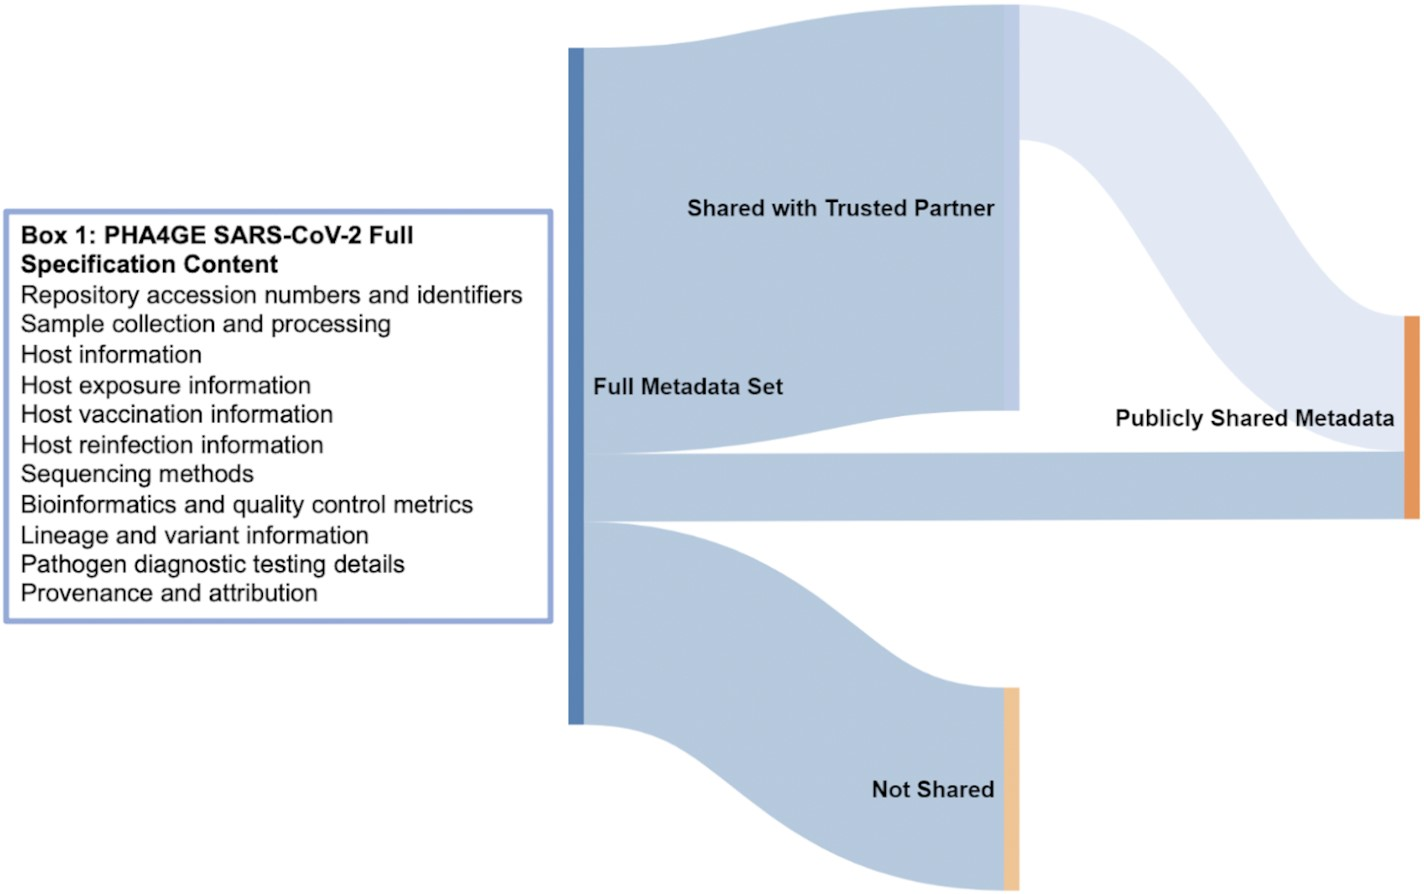
\includegraphics[width=\textwidth]{figures/chapter 7/giac003fig1.jpeg}
\caption{Contextual data flow. Contextual data can be captured and structured using the PHA4GE specification so that they can be more easily harmonized across different data sources and providers. Different subsets of the harmonized data can be (i) shared with public repositories, e.g., GISAID and INSDC; (ii) shared with trusted partners, e.g., national sequencing consortia, public health partners; and (iii) kept private and retained locally with the potential for sharing in the future for particular surveillance or research activities. While fields have been colour-coded in the template to indicate whether they are considered “required,” “strongly recommended,” or “optional,” how the specification is implemented and whether any of the data are shared is ultimately at the discretion of the user. Box 1 describes the information types covered in the full specification.}
\label{fig:chap7_figure_1}
\end{figure*}

The versioned specification is available as a contextual data collection template (.xlsx) and in machine-amenable JSON format from GitHub (v 3.0.0 - https://github.com/pha4ge/SARS-CoV-2-Contextual-Data-Specification) \cite{public_health_alliance_for_genomic_epidemiology_sars-cov-2-contextual-data-specification_nodate}. The collection template also offers standardized terms for a number of fields in the form of pick lists. The fields are colour-coded to indicate required (yellow), strongly recommended (purple) or optional status (white). Fields useful for surveillance were prioritized as required. Formats for data elements like dates are also prescribed according to international standards (e.g., dates should be formatted according to ISO8601).

The template is also supported by several materials such as term and field-level Reference Guides (available as tabs in the collection template Excel workbook), which provides definitions, data entry guidance and examples of usage \cite{public_health_alliance_for_genomic_epidemiology_sars-cov-2-contextual-data-specification_nodate}. The field-level Reference Guide also provides mapping of PHA4GE fields to existing contextual data standards, highlighting public health and SARS-CoV-2-specific fields that were missing as well as fields in those other standards that were considered out of scope. 

The Open Biological and Biomedical Ontology (OBO) Foundry is a community of researchers that use a prescribed set of principles and practices to develop a wide range of interoperable ontologies focused on the life sciences \cite{the_obo_foundry_obo_nodate}. Fields and terms in the specification have been mapped to existing OBO Foundry ontology terms, and where required, new ontology terms have been developed and are being made available in different application and domain-specific ontologies within The Foundry (see Table \ref{tab:ch7_table1} for a list of source ontologies). As of version 3.0.0 and beyond, terms in pick lists provided in the collection template are presented with corresponding ontology identifiers in the format “Label [ontology ID]” e.g., Blood [UBERON:0000178]. Axioms and additional cross references to ontologies and existing standards are actively being developed in collaboration with community developers. We anticipate that our contributions to these freely available, open-source resources will be of use to the COVID-19 research community.

\begin{table}[h!]
\caption{Ontologies implemented in the PHA4GE SARS-CoV-2 specification.}
\label{tab:ch7_table1}
\resizebox{\textwidth}{!}{%
\begin{tabular}{@{}ll@{}}
\toprule
Ontology$^1$                                    & Link                                           \\ \midrule
BRENDA Tissue Ontology (BTO)                 & https://obofoundry.org/ontology/bto.html       \\
Cell Line Ontology (CLO)                     & https://obofoundry.org/ontology/clo.html       \\
Environmental conditions,   treatments and exposures ontology (ECTO) & https://obofoundry.org/ontology/ecto.html   \\
Environment Ontology (ENVO)                  & https://obofoundry.org/ontology/envo.html      \\
Food Ontology (FoodOn)                       & https://obofoundry.org/ontology/foodon.html    \\
Gazetteer Ontology (GAZ)                     & https://obofoundry.org/ontology/gaz.html       \\
Gender, Sex, and Sexual Orientation Ontology (GSSO)                  & https://obofoundry.org/ontology/gsso.html   \\
Genomic Epidemiology Ontology (GenEpiO)      & https://obofoundry.org/ontology/genepio.html   \\
Genomics Cohorts Knowledge Ontology (GECKO)  & https://obofoundry.org/ontology/gecko.html     \\
Human Disease Ontology (DOID)                & https://obofoundry.org/ontology/doid.html      \\
Human Phenotype Ontology (HP)                & https://obofoundry.org/ontology/hp.html        \\
Mammalian Phenotype Ontology (MP)            & https://obofoundry.org/ontology/mp.html        \\
Measurement Method Ontology (MMO)            & https://obofoundry.org/ontology/mmo.html       \\
Mondo Disease Ontology (MONDO)               & https://obofoundry.org/ontology/mondo.html     \\
Mouse Pathology Ontology (MPATH)             & https://obofoundry.org/ontology/mpath.html     \\
National Cancer Institute Thesaurus (NCIT)   & https://obofoundry.org/ontology/ncit.html      \\
NCBI Taxonomy Ontology (NCBITaxon)           & https://obofoundry.org/ontology/ncbitaxon.html \\
Neuro Behaviour Ontology (NBO)               & https://obofoundry.org/ontology/nbo.html       \\
Ontology for Biomedical Investigations (OBI) & https://obofoundry.org/ontology/obi.html       \\
Ontology of Medically Related Social Entities (OMRSE)                & https://obofoundry.org/ontology/omrse.html  \\
Population and Community Ontology (PCO)      & https://obofoundry.org/ontology/pco.html       \\
UBERON Multi-species Anatomy Ontology (UBERON)                       & https://obofoundry.org/ontology/uberon.html \\
Unit Ontology (UO)                           & https://obofoundry.org/ontology/uo.html        \\
Vaccine Ontology (VO)                        & https://obofoundry.org/ontology/vo.html        \\ \bottomrule
\end{tabular}%
}
\item $^1$ Vocabulary for fields and terms in the specification have been sourced or mapped to OBO Foundry domain and application ontologies, which are highlighted in this list. New fields and terms for which there were no existing equivalents have been developed and submitted to these ontologies, expanding these community resources
\end{table}

Protocols have also been created and are openly available on protocols.io \cite{public_health_alliance_for_genomic_epidemiology_pha4ge_nodate}, including a curation Standard Operating Procedure (SOP) containing instructions for using the collection template as well as guidance for a number of privacy and practical concerns. A series of versioned SARS-CoV-2 sequence and contextual data submission protocols and accompanying instructional videos for how to prepare submissions and navigate through the various submission portals for GISAID, NCBI and EMBL-EBI are also provided.

A mapping file indicating which PHA4GE fields correspond to contextual data elements recommended by the World Health Organization has been provided to help data providers comply with international guidance \cite{world_health_organization_guidance_nodate}. This mapping file also includes tabs indicating which PHA4GE fields correspond to those found in different repository submission forms to facilitate data transformations for submissions. Such transformations can be automated using a contextual data harmonization application called the DataHarmonizer \cite{hsiao_public_health_bioinformatics_lab_dataharmonizer_2022}. PHA4GE has worked with the developers of the DataHarmonizer to offer the PHA4GE standard as a template in the tool (Gill et al, in preparation). Users can standardize and validate entered data and export it as GISAID and NCBI-ready submission forms (BioSample, SRA, GenBank and GenBank source modifier forms). It should be noted that other excellent contextual data transformation tools have been developed by the community, such as METAGENOTE, multiSub, and a GISAID-to-ENA conversion script \cite{noauthor_metagenote_nodate, haeussler_multisub_2022, noauthor_ena-content-dataflowscriptsgisaid_to_ena_nodate}.

A table outlining the different specification package materials can be found in Table \ref{tab:ch7_table2}.


\begin{longtable}{@{}lll@{}}
\caption{Resources that form the PHA4GE SARS-CoV-2 contextual data specification package}
\label{tab:ch7_table2}\\
Resource1 &
  Description &
  Link \\
\endfirsthead
%
\endhead
%
Collection   template and controlled vocabulary pick lists &
  Spreadsheet-based   collection form containing different fields (identifiers and accessions,   sample collection and processing, host information, host exposure,   vaccination and reinfection information, lineage and variant information,   sequencing, bioinformatics and QC metrics, diagnostic testing information,   author acknowledgements). Fields are colour-coded to indicate required,   recommended or optional status. Many fields offer pick lists of controlled   vocabulary. Vocabulary lists are also available in a separate tab. &
  https://github.com/pha4ge/SARS-CoV-2-Contextual-Data-Specification/raw/master/PHA4GE\%20SARS-CoV-2\%20Contextual\%20Data\%20Template.xlsx \\
Reference   guides &
  Field and   term definitions, guidance, and examples are provided as separate tabs in the   collection template .xlsx file (see Term Reference Guide and Field Reference   Guide). &
  https://github.com/pha4ge/SARS-CoV-2-Contextual-Data-Specification/raw/master/PHA4GE\%20SARS-CoV-2\%20Contextual\%20Data\%20Template.xlsx \\
Curation   protocol on protocols.io &
  Step-by-step   instructions for using the collection template are provided in a standard   operating procedure (SOP). Ethical, practical, and privacy considerations are   also discussed. Examples and instructions for structuring sample descriptions   as well as sourcing additional standardized terms (outside those provided in   pick lists) are also discussed. &
  dx.doi.org/10.17504/protocols.io.btpznmp6 \\
Mapping   file of PHA4GE fields to metadata standards &
  PHA4GE   fields are mapped to existing metadata standards such as the Sample   Application Standard, MIxS 5.0, and the MIGS Virus Host-associated attribute   package. Mappings are available in the Reference guide tab. Mappings   highlight which fields of these standards are considered useful for SARS-CoV-2   public health surveillance and investigations, and which fields are   considered out of scope. &
  https://github.com/pha4ge/SARS-CoV-2-Contextual-Data-Specification/raw/master/PHA4GE\%20SARS-CoV-2\%20Contextual\%20Data\%20Template.xlsx \\
Mapping   of PHA4GE fields to WHO metadata recommendations &
  PHA4GE   fields are mapped to corresponding contextual data elements recommended by   the World Health Organization. &
  https://github.com/pha4ge/SARS-CoV-2-Contextual-Data-Specification/raw/master/PHA4GE\%20to\%20Sequence\%20Repository\%20Field\%20Mappings.xlsx \\
Mapping   file of PHA4GE fields to EMBL-EBI, NCBI and GISAID submission requirements &
  Many   PHA4GE fields have been sourced from public repository submission   requirements. The different repositories have different requirements and   field names. Repository submission fields have been mapped to PHA4GE fields   to demonstrate equivalencies and divergences. &
  https://github.com/pha4ge/SARS-CoV-2-Contextual-Data-Specification/raw/master/PHA4GE\%20to\%20Sequence\%20Repository\%20Field\%20Mappings.xlsx \\
Data submission protocol (NCBI) on protocols.io &
  The   SARS-CoV-2 submission protocol for NCBI provides step-by-step instructions   and recommendations aimed at improving interoperability and consistency of   submitted data. &
  dx.doi.org/10.17504/protocols.io.bui7nuhn \\
Data submission protocol (EMBL-EBI) on protocols.io &
  The   SARS-CoV-2 submission protocol for ENA provides step-by-step instructions and   recommendations aimed at improving interoperability and consistency of   submitted data. &
  dx.doi.org/10.17504/protocols.io.buqnnvve \\
Data   submission protocol (GISAID) on protocols.io &
  The   SARS-CoV-2 submission protocol for GISAID provides step-by-step instructions   and recommendations aimed at improving interoperability and consistency of submitted   data. &
  dx.doi.org/10.17504/protocols.io.bumknu4w \\
JSON   structure of PHA4GE specification &
  A JSON   structure of the PHA4GE specification has been provided for easier   integration into software applications. &
  https://raw.githubusercontent.com/pha4ge/SARS-CoV-2-Contextual-Data-Specification/master/PHA4GE\_SARS-CoV-2\_Contextual\_Data\_Schema.json \\
PHA4GE   template in the DataHarmonizer &
  Javascript   application enabling standardized data entry, validation and export of   contextual data as submission-ready forms for GISAID and NCBI. The SOP for   using the software can be found at   https://github.com/Public-Health-Bioinformatics/DataHarmonizer/wiki/PHA4GE-SARS-CoV-2-Template &
  https://github.com/Public-Health-Bioinformatics/DataHarmonizer/releases
  
\item $^1$ There are a number of resources that form the PHA4GE SARS-CoV-2 contextual data specification package which are described in the table. The package has been compiled to support user implementation and data sharing, with integration into workflows and new software applications in mind.
\end{longtable}



\newpage
\section{References}
\printbibliography[heading=none]
\end{refsection}

%-----------------------------------------------------------------
% Conclusion
%-----------------------------------------------------------------
\newpage
\chapter{Conclusion \label{ch:conclusion}}
\thispagestyle{empty}
\newpage
\mbox{}\\
\vspace{8cm}

The work I hereby present aims to evaluate the use of bioinformatics methods for the analysis of metagenomic data to allow the rapid identification, virulence analysis and antimicrobial susceptibility prediction of pathogens with clinical relevance. \ac{SMg} still presents as a promising methodology to obtain very fast results for the identification of pathogens and their virulence and resistance properties directly from samples, without the need for culture. 
To be accredited and used in clinical settings, this approach must be standardised and the statistical metrics used to analyse and report the data must be validated.

The impact and applicability of \ac{SMg} in clinical microbiology, including both a diagnosis and surveillance and infection prevention, has been assessed, with the unique challenges of both highlighted. For diagnostics, the biggest drawback of this methodology is the extremely cost-ineffective negative results, allied with the very high sensitivity that translates into several false-positive results. It has been used as a last-resort diagnostic technique \citep{he_case_2022, vijayvargiya_application_2019, sanabria_shotgun-metagenomics_2020, hirakata_application_2021}, with great success when classical approaches fail to detect the causative agent of a disease. Chapter \ref{ch:paper1} aimed to evaluate \ac{SMg} approaches in a collection of varied samples, with particular interest in the bioinformatic pipeline applied, and how it affected the results obtained in a potential diagnosis setting. Most pathogens identified by culture were also identified through metagenomics, but substantial differences were noted between the taxonomic classification tools. In surveillance and infection prevention, \ac{SMg} has also been successfully applied \citep{loman_culture-independent_2013, huang_metagenomics_2017, li_microbiome_2021}, with programs existing relying on this methodology for the monitoring of emerging or of global interest pathogens \citep{ko_metagenomics-enabled_2022}. Chapter \ref{ch:paper2}, the novel detection of an \textit{mcr}-5 gene, named \textit{mcr}-5.4, is reported, from a concentrated water sample. 

The accurate identification of pathogens of interest from \ac{SMg} remains one of the biggest challenges when analysing this type of data. A hybrid approach of read mapping and \textit{de novo} assembly methods sometimes proved the only way to successfully recover sequences of interest with enough quality for genome reconstruction. In Chapter \ref{ch:paper3}, both approaches were employed to provide, in a single methodological step, identification and characterization of a whole viral genome at the nucleotide level. Furthermore, Chapter \ref{ch:paper4} highlighted that no assembler stood out as an undisputed all-purpose choice for short-read metagenomic prokaryote genome assembly, hence efforts are still needed to further improve metagenomic assembly performance. 

A strong focus on  the standardisation and reproducibility of the results obtained, with the employment of new technologies to do so, such as container software and workflow managers, is of the uttermost necessity for the \ac{SMg} data analysis solutions. Transparency, scalability, and ease of installation are key-stones, regardless of the tools chosen. The solutions adopted throughout this work, such the use of docker, nextflow and conda, allied to clear and easy to follow documentation, aim to lower the barrier of entry when performing detailed analysis that are complex and computationally expensive in their nature. But most importantly, the production of intuitive, responsive and easy-to-follow reports, allowing the summary of key results, as well as the detailed exploration of the resulting data, by stakeholders, be it bioinformatic personnel or experts in the given area of expertise, represent the single most important contribution to lowering the barrier between who produces the data and who has the capacity to make informed decisions based on that data.   

As public health laboratories expand their genomic sequencing and bioinformatics capacity for the surveillance of different pathogens, labs must carry out robust validation, training, and optimisation of wet- and dry-lab procedures. Despite this richness in genomic information, the same is not observed for the contextual information that accompanies it. This contextual information, composed of metadata  Standardisation of harmonisable, publicly available community standards is ultimately what will allow the transmission of information through various stakeholders, containing the minimum information required for it to be understandable and actionable across domains. 

\section{Future perspectives}

Despite the results presented in this work, the future of \ac{SMg} still looks promising. Regardless, for it to pass from the last resort solution when traditional methods fail to a standard in clinical microbiology, some issues still need to be addressed. 

One of the biggest hinders to the application of \ac{SMg} in the clinic is the significant cost of negative results, allied with a very high sensitivity but not as high specificity, being very prone to contamination leading to false positive results. Therefore, part of the work to improve this technology passes through the improvement in the bench. Host depletion steps still have a long way to produce satisfactory results for diagnosis purposes, without altering the proportions of organisms in a community. Although traditional methods require a very significant amount of man-hours, sequencing requires a different, more specialised set of skills to obtain quality results. Additionally, the time gained in the results attainment is offset by the increased cost. 

Regarding bioinformatic analysis of \ac{SMg} data, the lack of golden standards presents the biggest hindrance. But as new methods keep being developed, fuelled by the extreme and exciting interest of the community for this methodology, and more importantly, as current methods continue to be validated, and their results openly shared, in a faindable and FAIRer way, we slowly but surely walk towards the standardisation of methodologies. 

I'm as excited with the potential of \ac{SMg} for clinical microbioly, both in the diagnostics and public health and surveillance branches, as I was when I first started this project. The potentials are staggering, albeit currently it's still very much an experimental and/or last resort approach. As methodologies continue to improve, sequencing will become ubiquitous in every diagnostics and public health laboratory. The transition between academic applications to being a viable solution in hospitals and health reference laboratories might be slow, or at least slower than what was once expected, but it's an inevitability that we should not only be prepared for but also excited about. 

%-----------------------------------------------------------------
% Appendix
%-----------------------------------------------------------------
\appendix
\chapter{Appendix}
\include{chapters/appendix}

\includepdf[pages={1-}]{resources/papers/s41598-018-31873-w.pdf}
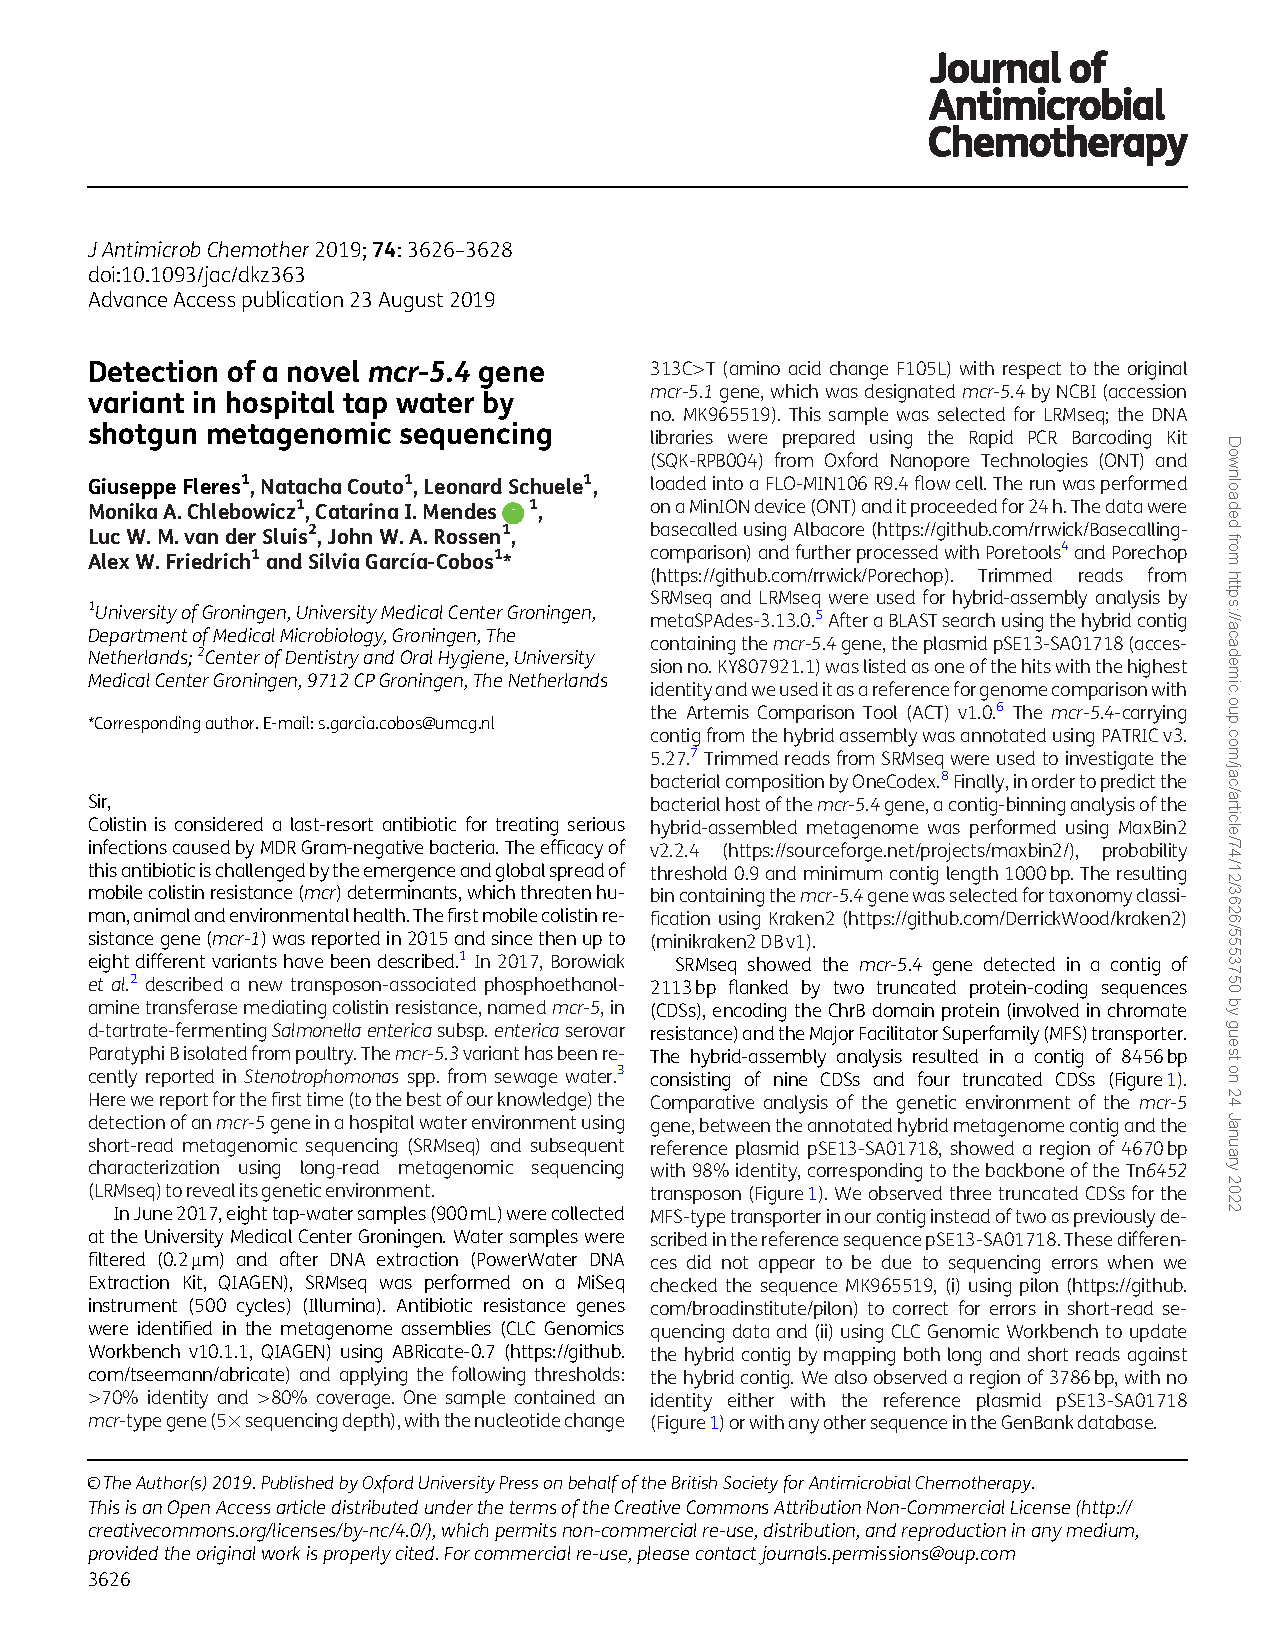
\includepdf[pages={1-}]{resources/papers/dkz363.pdf}
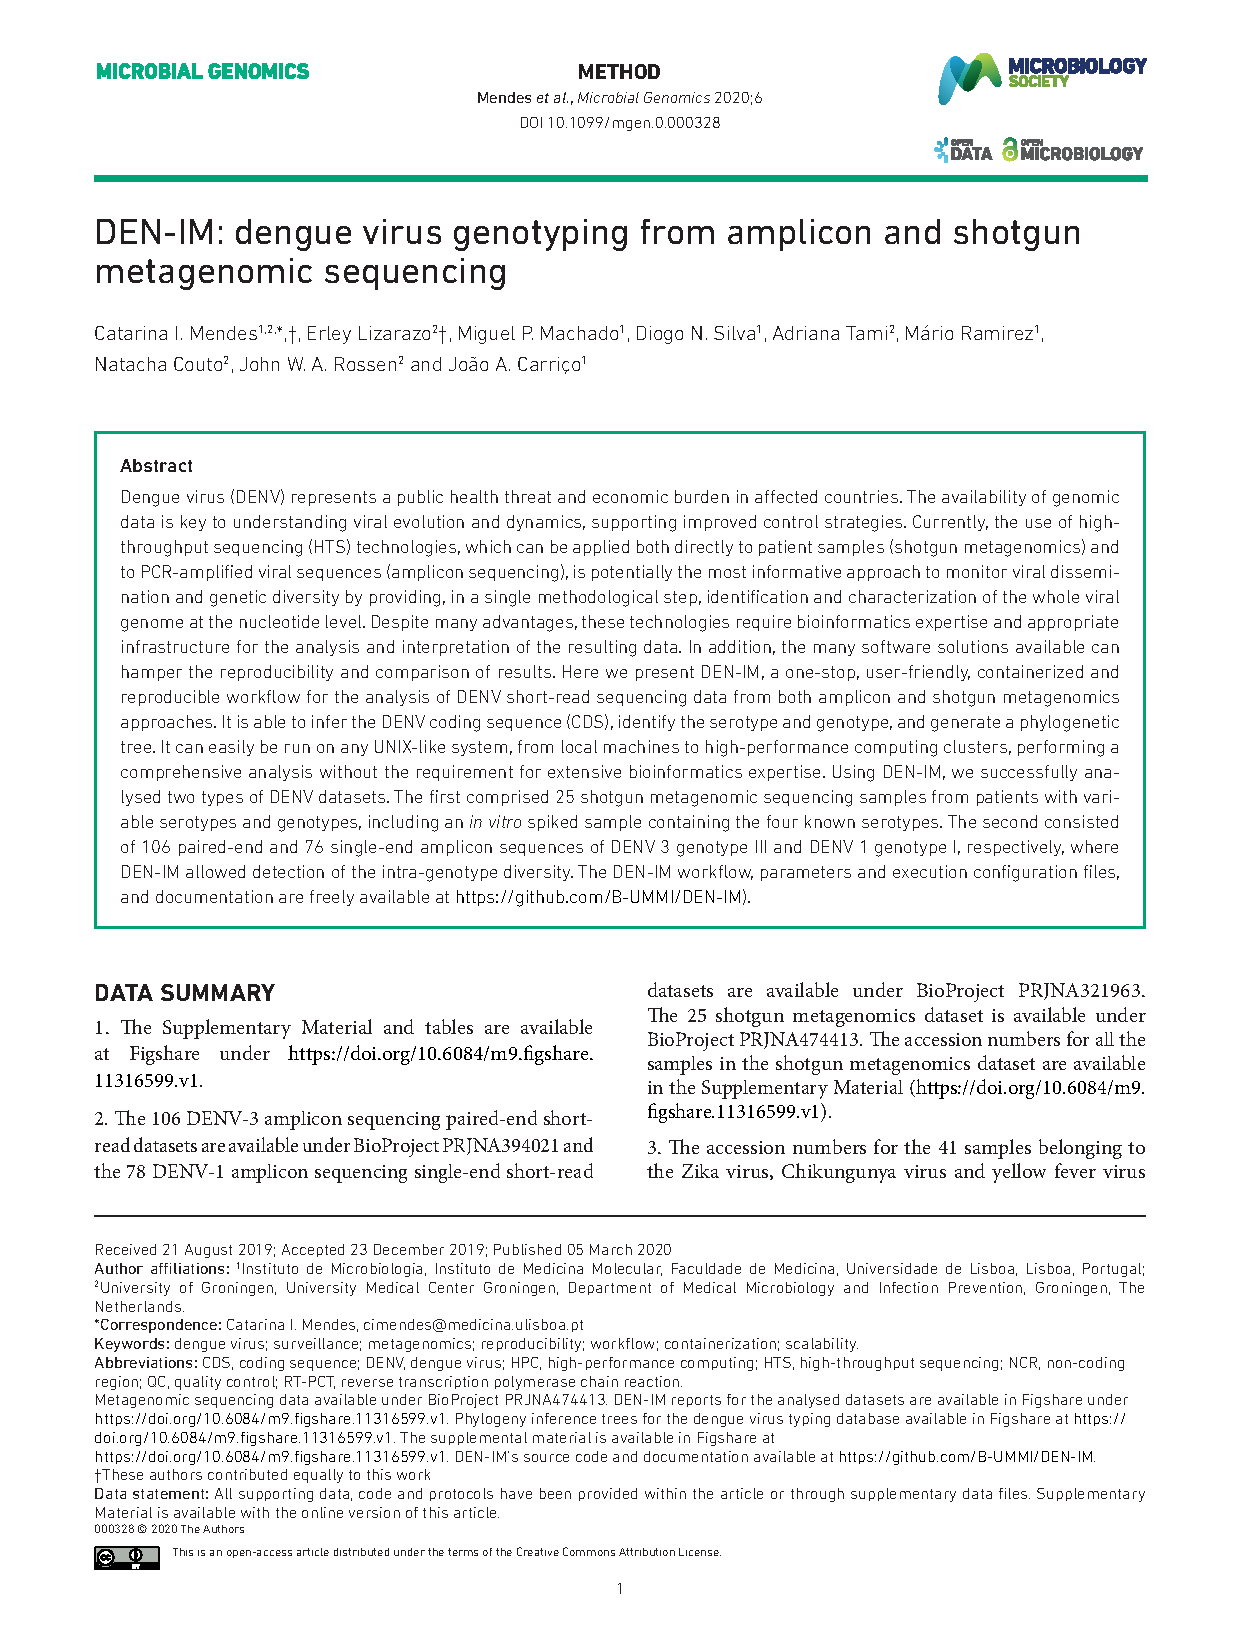
\includepdf[pages={1-}]{resources/papers/mgen000328.pdf}

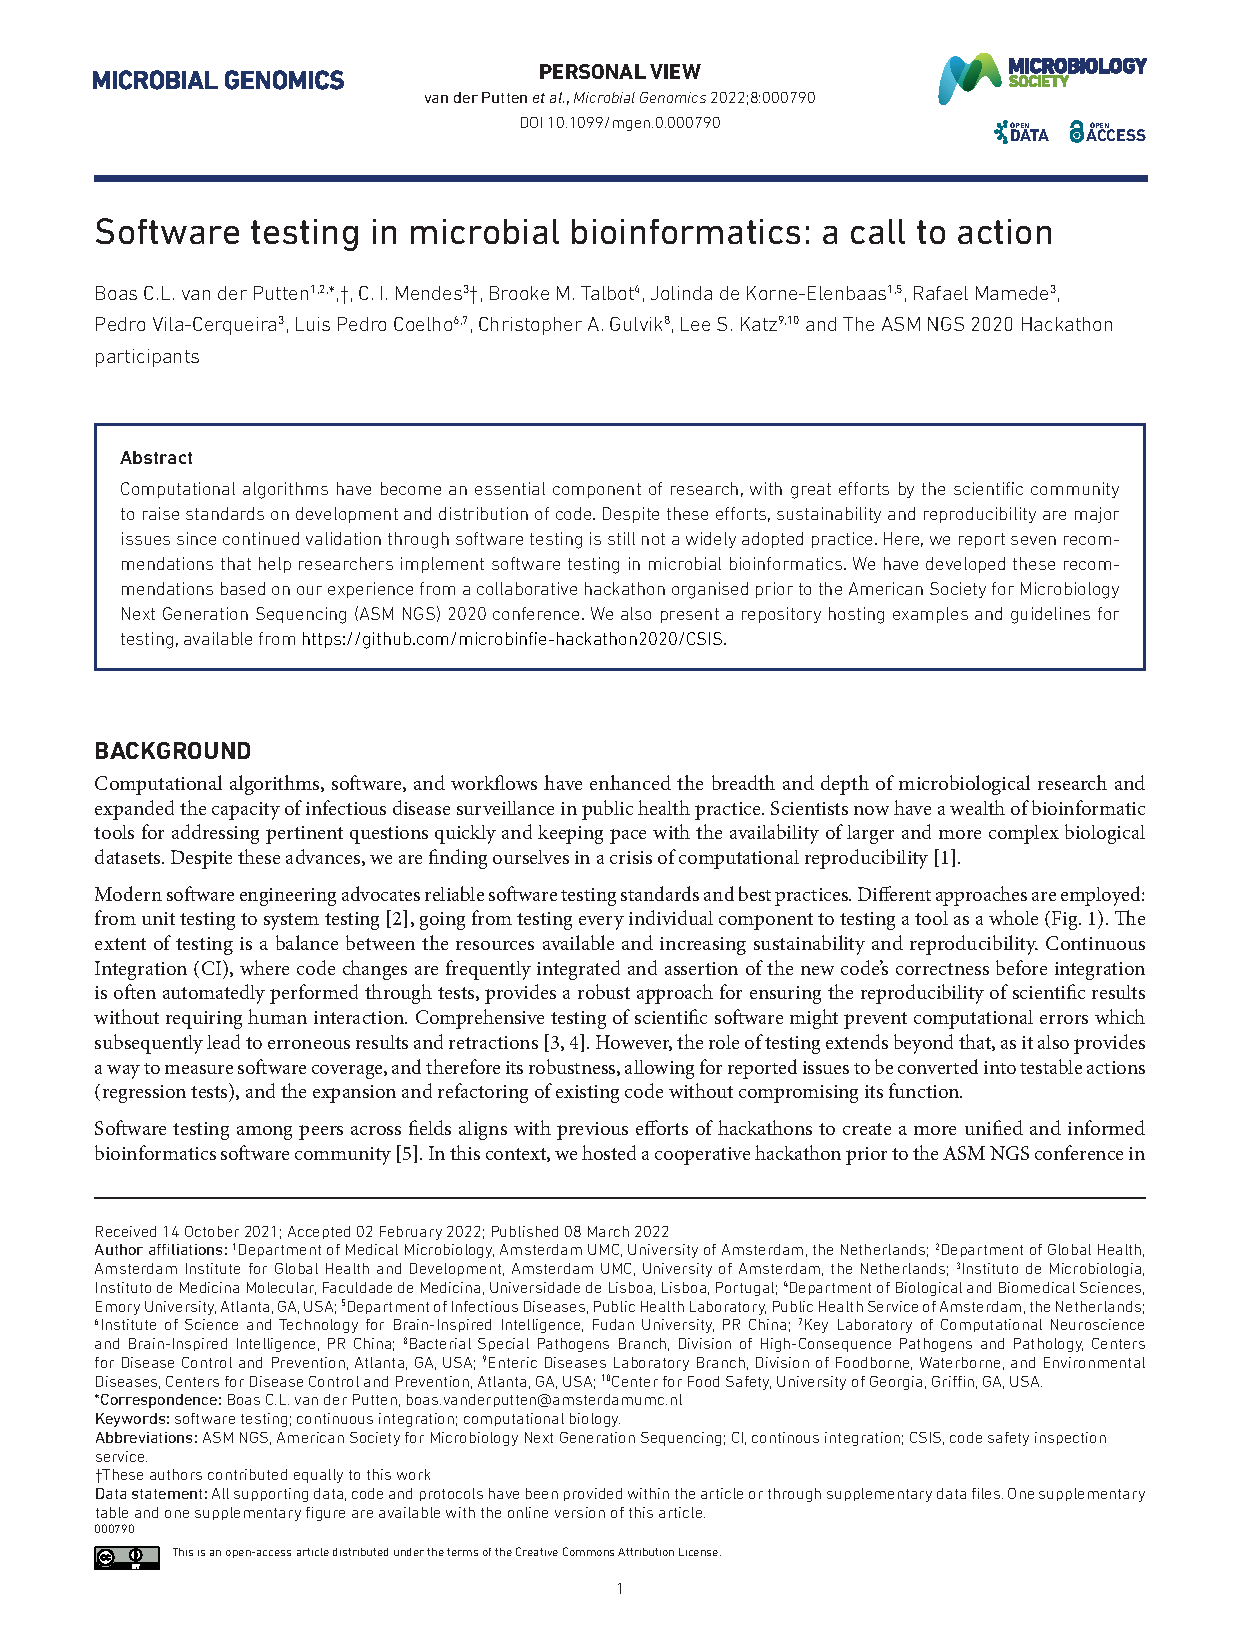
\includepdf[pages={1-}]{resources/papers/mgen000790.pdf}

\end{sloppy}
\end{document}
